\documentclass[11pt]{article}
\pdftrailerid{}
\usepackage[a4paper,margin=28mm]{geometry}
\usepackage{amsmath,amssymb,amsthm,mathtools,bm}
\usepackage[T1]{fontenc}
\usepackage{lmodern,microtype}
\usepackage{graphicx,tikz,booktabs,array,longtable}
\usetikzlibrary{arrows.meta,positioning,calc}
\usepackage[numbers,sort&compress]{natbib}
\usepackage[colorlinks=true,linkcolor=blue,citecolor=blue,urlcolor=blue]{hyperref}
\usepackage{bookmark}
\makeatletter
\renewcommand*\l@subsection{\@dottedtocline{2}{1.5em}{3.2em}}
\makeatother
\hypersetup{pdftitle={Compatibility entropy and the spectrum of a Thorp sweep},pdfauthor={OpenAI}}
\newtheorem{theorem}{Theorem}[section]
\newtheorem{lemma}[theorem]{Lemma}
\newtheorem{proposition}[theorem]{Proposition}
\newtheorem{corollary}[theorem]{Corollary}
\theoremstyle{definition}
\newtheorem{definition}[theorem]{Definition}
\theoremstyle{remark}
\newtheorem{remark}[theorem]{Remark}
\DeclareMathOperator{\Tr}{Tr}
\DeclareMathOperator{\KL}{KL}
\DeclareMathOperator{\Sym}{Sym}
\DeclareMathOperator{\Var}{Var}
\DeclareMathOperator{\Ent}{Ent}
\newcommand{\TV}{\mathrm{TV}}
\newcommand{\HS}{\mathrm{HS}}
\newcommand{\op}{\mathrm{op}}
\newcommand{\E}{\mathbb E}
\newcommand{\PP}{\mathbb P}
\newcommand{\id}{\mathrm{id}}
\newcommand{\eps}{\varepsilon}
\newcommand{\ind}{\mathbf1}
\allowdisplaybreaks[1]
\setlength{\emergencystretch}{2em}
\title{Compatibility entropy and the spectrum of a Thorp sweep}
\author{OpenAI}
\date{September 26, 2026}
\begin{document}
\maketitle
\begin{abstract}
We prove that the Thorp shuffle on $n=2^d$ cards mixes in $\Theta(d)$ physical shuffles. After a sufficiently large fixed number of coordinate sweeps, the total-variation distance of the full permutation from uniform tends to zero as $d\to\infty$.
\end{abstract}
\begingroup
\small
\tableofcontents
\endgroup
\clearpage
\section{Introduction}
A single coordinate sweep of the Thorp shuffle sends each card to a uniform position. This marginal statement leaves open the correlations among cards that have used the same switches. Those correlations are the object of this paper. We ask how much simultaneous row and column structure a permutation can retain, and how that restriction controls all the singular values of the sweep.

Let $n=2^d$ and identify the positions with $\{0,1\}^d$. A sweep visits the coordinates in order. At a visit it independently swaps, with probability $1/2$, the two cards on each edge in that coordinate direction. Write $T_n$ for its convolution operator on $\ell^2(S_n)$. One sweep is $d$ physical Thorp shuffles after removing the deterministic rotation of coordinates; Section~\ref{sec:prelim} gives the exact convention. The adjoint reverses the coordinate order. Thus $T_n^*T_n$ is a positive operator for a forward sweep followed by a reverse sweep, with fresh independent switches. Powers of $T_n$ instead describe repeated forward sweeps.

Thorp introduced the shuffle in 1973 while studying imperfect shuffling in Faro; his original description already makes the independent pair choices explicit~\cite[Section~3.1]{Thorp1973}. The distinction between one card and the whole deck is fundamental. One sweep uses $nd/2$ random bits, whereas a uniform permutation has entropy $\log_2(n!)$ bits. More generally, the support after $t$ physical shuffles has size at most $2^{tn/2}$, giving the lower bound $2d-O(1)$ for fixed-error mixing. Uniformity of every one-card marginal therefore leaves a substantial global problem.

The first polylogarithmic full-deck bound was Morris's $O(d^{44})$ theorem, announced in 2005 and published in 2008~\cite{Morris2008}. Montenegro and Tetali sharpened its evolving-set analysis to $O(d^{29})$~\cite[Section~6.4, Theorems~6.14--6.15]{MontenegroTetali2006}. Morris then introduced entropy contraction arguments giving $O((\log n)^4)$ shuffles for every even deck size~\cite{Morris2009}, and $O(d^3)$ for $n=2^d$~\cite{Morris2013}. These comparisons count physical shuffles at fixed total-variation error. The present paper obtains $\Theta(d)$ mixing for power-of-two decks from a stronger statement about the entire singular spectrum of one sweep. The upper bound uses a fixed number of complete sweeps.

Partial-card laws lead to a related but different question. Morris, Rogaway and Stegers obtained bounds for designated labeled cards and used them to analyze enciphering on small domains~\cite{mrs,MorrisRogawayStegers2018}. Czumaj and V\"ocking proved mixing of any fixed fraction less than one of the labeled cards after $O((\log n)^2)$ ordinary Thorp shuffles~\cite{CzumajVocking2014}. Their passage to a full random permutation uses additional indistinguishable cards which are discarded afterward. Czumaj also constructed switching networks that mix a full permutation with $O(n\log n)$ switches and $O((\log n)^2)$ depth~\cite{Czumaj2015}. These results explain the importance of shared-switch correlations beyond individual marginals; their state spaces or networks differ from the ordinary full-deck chain studied here.

Splitting the coordinate list in half identifies the positions with a rectangle. The first part of the sweep acts independently within its rows and the second independently within its columns. This is a recursion into smaller sweeps, but its two symmetry decompositions do not commute. We measure this obstruction by the following concrete event.

Take an $A$-by-$D$ rectangle with $AD=n$, and let $R=(S_D)^A$ and $C=(S_A)^D$ be its row and column permutation groups. A row permutation $r=(r_i)$ followed by a column permutation $c=(c_k)$ sends $(i,j)$ to $(c_{r_i(j)}(i),r_i(j))$. We call $(r,c)$ \emph{compatible} if this permutation can also be performed by a column permutation followed by a row permutation. Equivalently, for each original column $j$, the $A$ values $c_{r_i(j)}(i)$ are distinct. The opposite-order factorization, if it exists, is unique. Let $\mathcal I\subset R\times C$ denote this event and let $U$ denote independent uniform permutations in all the lines.

\begin{figure}[ht]
\centering
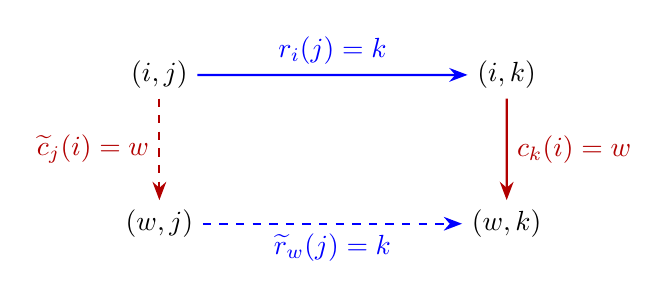
\begin{tikzpicture}[>=Stealth,scale=1.05]
\node (ij) at (0,1.8) {$(i,j)$};
\node (ik) at (4.2,1.8) {$(i,k)$};
\node (wj) at (0,0) {$(w,j)$};
\node (wk) at (4.2,0) {$(w,k)$};
\draw[->,thick,blue] (ij) -- node[above] {$r_i(j)=k$} (ik);
\draw[->,thick,red!70!black] (ik) -- node[right] {$c_k(i)=w$} (wk);
\draw[->,thick,red!70!black,dashed] (ij) -- node[left] {$\widetilde c_j(i)=w$} (wj);
\draw[->,thick,blue,dashed] (wj) -- node[below] {$\widetilde r_w(j)=k$} (wk);
\end{tikzpicture}

\caption{The two routings of one labeled position. The solid route uses a row permutation and then a column permutation. Compatibility means that the dashed routes of all positions can be assembled into column and row permutations; this is exactly the distinctness condition for the values $w$ in each original column $j$.}
\label{fig:compatibility}
\end{figure}

The first main result allows weights on every line. It retains the cost of marginal concentration instead of assuming the line laws remain uniform after compatibility is imposed.
\begin{theorem}[Weighted compatibility]\label{tra:duality:weighted}\label{tra:duality:weighted-statement}
There are absolute constants $L,C_0>0$ such that the following holds. Put $m=\sqrt n$, assume $m/2\le A,D\le2m$, and take $m$ sufficiently large that $\theta=1-L/\log m>0$. For all nonnegative functions $w_i:S_D\to[0,\infty)$ and $v_k:S_A\to[0,\infty)$,
\begin{equation}\label{tra:duality:eq5}
 \frac{n!}{|R||C|}\,
 \mathbb E_U\!\left[\mathbf1_{\mathcal I}
       \prod_{i=1}^A w_i(r_i)\prod_{k=1}^D v_k(c_k)\right]
 \le e^{C_0n^{.54}}
       \prod_{i=1}^A(\mathbb E w_i^{1/\theta})^\theta
       \prod_{k=1}^D(\mathbb E v_k^{1/\theta})^\theta .
\end{equation}
The expectations on the right are uniform on the indicated symmetric groups, and logarithms are natural.
\end{theorem}
The factor $n!/(|R||C|)$ is forced by regular trace normalization. Its leading logarithm is $n$. The entropy argument supplies a compatibility cost with leading logarithm $-n$, so those terms cancel. What remains is small enough to be absorbed by the multiplicity of a large irreducible representation.

To state the resulting spectral estimate, write $T_{n,\lambda}$ for the Fourier matrix on one copy of the irreducible representation of $S_n$ indexed by $\lambda\vdash n$, and let $D_\lambda$ be its dimension. Throughout, traces and Schatten norms are unnormalized. For $p>0$, the ordinary regular trace is
\[
 Z_n(p)=\Tr_{\mathrm{reg}}(T_n^*T_n)^p
       =\sum_{\lambda\vdash n}D_\lambda
                 \Tr(T_{n,\lambda}^*T_{n,\lambda})^p.
\]
The factor $D_\lambda$ records the number of copies in the regular representation.
\begin{theorem}[A bounded regular moment]\label{tra:duality:moment}
There is an absolute finite $p_*>0$ such that, for every dyadic $n$,
\begin{equation}\label{tra:duality:eq7}
 Z_n(p_*)\le1+\frac1{16}.
\end{equation}
For every integer $M\ge p_*$, $M$ independent forward sweeps have worst-start total-variation distance at most $1/8$ from uniform.
\end{theorem}
The moment records both the size and the number of nonconstant singular values. Its concrete consequences are as follows; Section~\ref{sec:spectral-conversion} proves the conversion with the regular multiplicities included.
\begin{corollary}[Singular ranks and full-deck mixing]\label{cor:intro-consequences}
For every nontrivial $\lambda\vdash n$ and $1\le r\le D_\lambda$,
\[
 s_r(T_{n,\lambda})\le(16D_\lambda r)^{-1/(2p_*)}.
\]
If $s_j(T_n)$ denotes the full regular singular list, including all multiplicities and zeros, then
\[
 s_j(T_n)\le j^{-1/(2p_*)}\qquad(1\le j\le n!).
\]
The constant singular value is the first value. The physical Thorp chain has worst-start $1/4$ mixing time $\Theta(d)$; more precisely its lower bound is $2d-O(1)$. For every fixed integer $M>p_*$, the worst-start total-variation distance after $Md$ physical shuffles tends to zero as $d\to\infty$.
\end{corollary}
The lower bound uses only support size. The upper bounds use the regular moment and Schatten H\"older for the matrix product $T_n^M$. They do not require the sweep to be normal. The sign block vanishes, and the dimensions of the remaining nonconstant blocks tend to infinity; the extra power when $M>p_*$ therefore makes the error vanish. The proof does not optimize the constant multiplying $d$ or establish a cutoff profile.

\paragraph{The first complete proof.}
Section~\ref{tra:duality} proves both theorems without using any of the later recursions. It starts with the exceptional representations, those whose Young diagram has a long first row. Such a representation first appears on ordered tuples of a corresponding number of cards. Subtracting all smaller-tuple kernels cancels every path configuration with an isolated card. The remaining configurations contain a forest of interactions. The probability of each forest edge, together with a deterministic bound on shared switches, gives the required sparse estimate.

For the other representations, the proof returns to the rectangle. Under an arbitrary law supported on compatible pairs, expose the row permutations and then the column permutations in a random order. Each light, unclumped entry costs nearly one nat because previously exposed columns forbid values. Repeated row images and large atoms of the local prediction are excluded from this calculation; their losses are charged to the corresponding marginal relative entropies. The resulting inequality still retains nearly the full sum of marginal deficits. Entropy duality then gives Theorem~\ref{tra:duality:weighted}.

The final step is analytic. A positive-matrix trace inequality reduces a singular moment to four alternating row and column factors. The identity coefficient of that product is exactly a weighted compatibility sum. Inverse Hausdorff--Young bounds its line weights by the smaller sweeps' moments. This first gives a subexponential bound on the regular trace. Each singular value in a large-dimensional irreducible occurs many times, so a small increase in the moment exponent makes that part of the trace small. The sparse estimate treats the remaining part. The exponent increases by $1+O(1/d)$ at a split into approximately $d/2$ coordinates; the product of these increases stays bounded.

\paragraph{The additional estimates.}
Sections~\ref{sec:prelim}--\ref{sec:spectral-conversion} contain the common conventions, the first complete proof, and the conversion to ranks and mixing. The subsequent arguments provide alternative proofs and several finer estimates. Some capped or weighted compatibility bounds already follow from Theorem~\ref{tra:duality:weighted}; their separate proofs offer different ways to expose the grid. The conditional correlation, exceptional-set, sparse representation and level estimates retain further structure, as described below.

The first group refines the entropy at the middle split. Section~\ref{tra:conditional} keeps conditional column deficits after the row array is known, together with projection ranks. Sections~\ref{tra:inverse-color}--\ref{tra:fractional-density} successively use inverse-color availability, survival-tilted predictions, and fractional integrability of coefficient densities. These formulations permit different changes of measure while retaining a quantitative charge for the concentration of the line laws. Section~\ref{tra:asymmetric} permits a very unequal rectangle; fixed chunks of coordinates provide its sparse estimate.

A second group keeps track of representation structure. Section~\ref{tra:projection-deletion} estimates the loss of diagram level under matching deletion and restriction to two halves. Section~\ref{tra:first-interactions} organizes the sparse cancellation by first interactions. Section~\ref{tra:harmonic-overlaps} lifts harmonic functions from smaller tuples and bounds both operator and Hilbert--Schmidt overlaps. Section~\ref{tra:regular-ranks} carries the full regular singular list through its recursion, whereas Section~\ref{tra:collision-series} retains positive level sums weighted by dimensions of the tail tableaux. The collision generating function in the latter argument preserves positivity before the missing regular multiplicity is restored.

The final three sections develop further ways to cross the middle grid. In Section~\ref{sec:convex-grid}, a convex weight in the diagram level and logarithmic dimension compensates for levels lost under restriction. In Section~\ref{sec:band-grid}, a fourth-moment estimate for singular bands transfers a profile without summing those bands prematurely. Finally, Section~\ref{sec:smoothed-grid} constructs a positive operator series that majorizes arbitrary matrix-coefficient squares by densities whose low-level restrictions can be controlled pointwise. The bound holds for each line permutation, so it remains valid after conditioning on a complete compatible grid while the auxiliary Bernoulli subsets are still sampled independently. The proof uses a tableau restriction estimate and finite-lattice association, and then telescopes the costs of smoothing along the exposure.

\paragraph{Methodological context.}
The rectangular geometry has a close precedent in H\aa stad's square lattice shuffle, which alternates independent uniform permutations within all rows and within all columns~\cite{Hastad2006,Hastad2016}. The corrected theorem gives full-permutation mixing in a constant number of such layers. In the Thorp recursion each line is acted on by a smaller sweep. Thus the middle-grid estimate has to accept nonuniform line densities and their Fourier blocks. This is the purpose of the marginal entropy terms in Theorem~\ref{tra:duality:weighted}.

Random-order exposure belongs to the entropy method used by Radhakrishnan in his proof of Br\'egman's theorem and by Linial and Luria for high-dimensional permutation counting~\cite{Radhakrishnan1997,LinialLuria2014}. Our exposure estimates keep relative entropies of nonuniform marginal laws; we prove those estimates here. The passage from those deficits to weighted product inequalities is the finite-space entropy--Brascamp--Lieb duality of Carlen and Cordero-Erausquin~\cite[Theorem~2.1]{CarlenCorderoErausquin2009}. The operator transfer uses the Araki--Lieb--Thirring inequality~\cite{araki1990,audenaert2007} and the classical inverse Hausdorff--Young inequality, in the compact-group normalization stated in~\cite[Lemma~5.1(2)]{garcia-cuerva-parcet2004}. We specify their normalization at use. The representation arguments use branching, Pieri, the hook-length formula and the content formula in the conventions of Sagan, Stanley and Vershik--Okounkov~\cite{Sagan2001,Stanley1999,VershikOkounkov2005}.

The sparse estimates also use an occupied-set product inequality preserved by fair swaps. We prove the needed two-site calculation directly. It is consistent with the stronger preservation of negative dependence under partial symmetrization proved by Borcea, Br\"and\'en and Liggett~\cite[Theorems~4.9 and~4.20]{BorceaBrandenLiggett2009}. The pointwise smoothing argument uses the finite distributive-lattice association theorem of Fortuin, Kasteleyn and Ginibre~\cite[Proposition~1]{FortuinKasteleynGinibre1971}; the required tableau monotonicities and the subsequent operator construction are established here.

The companion on routing densities~\cite[Lemma~3.2]{OpenAIRouting2026} proves the deterministic contact lemma, with contacts counted as shared switches; we also give an entropy proof of its local form when it enters the sparse estimate. Counting both participating endpoints doubles that bound. All sparse probability estimates and entropy-to-spectrum closures needed here are proved in this paper. The short companion \emph{Optimal-order mixing of the Thorp shuffle}~\cite[Theorem~1.1]{OpenAIOptimal2026} uses conditional marginals and an eight-block representation lift to prove optimal-order mixing of the full deck. Its mixing theorem is not an input to the compatibility arguments here.

\section{The sweep, Fourier norms and common estimates}\label{sec:prelim}
We fix physical time and Fourier normalization, then record the
representation and positive-matrix estimates used throughout the paper.

\subsection{Binary positions and sweep operators}
Number positions by $x=(x_1,\ldots,x_d)\in\mathbb F_2^d$, most significant bit first. One shuffle sends
\[
 x\longmapsto(x_2,\ldots,x_d,x_1+\xi_{x_2,\ldots,x_d}),
\]
where the $2^{d-1}$ bits $\xi$ are independent and fair. Denote this physical-shuffle law by $q_d$, and define $t_{\mathrm{mix}}(d)$ to be the least time at which its worst-start total-variation distance from uniform is at most $1/4$. Write $R$ for the cyclic rotation and $h_t$ for the pair switches at physical time $t$, so the time-$t$ permutation is $Rh_t\cdots Rh_1$. Factoring out $R^t$ conjugates the switches into the successive coordinate directions. This deterministic left multiplication preserves distance to uniform. At time $d$, $R^d=I$, and one sweep has exactly the law of $d$ physical shuffles.

Permutations send each input position to its output. A product $gh$ applies $h$ first. For measures, $\mu*\nu$ denotes the law of $gh$ for independent $g\sim\mu,h\sim\nu$. In a unitary representation $\rho_\lambda$, define
\[
 \widehat\mu(\lambda)=\sum_g\mu(g)\rho_\lambda(g),
 \qquad\widehat{\mu*\nu}=\widehat\mu\,\widehat\nu.
\]
A fair switch layer averages the subgroup generated by its disjoint transpositions, and hence is an orthogonal projection $\Pi_i$. With chronological coordinate order $1,\ldots,d$, put
\[
 T_n=\Pi_d\cdots\Pi_1,\qquad Q_n=T_n^*T_n,
 \qquad P_n=T_nT_n^*,\qquad n=2^d.
\]
Both positive squares have the same singular spectrum, including zero multiplicities; they correspond to opposite chronological orientations.
\begin{lemma}[Annihilated shapes]\label{lem:annihilation}
The sign representation is annihilated by every nonempty fair layer. Every irreducible of $S_n$ indexed by a shape with more than $n/2$ rows is annihilated by a sweep.
\end{lemma}\begin{proof}
The sign average contains a fair transposition. For the second assertion, by Young's rule, the permutation module induced from the trivial representation of $(S_2)^{n/2}$ has only shapes dominating $(2^{n/2})$, hence at most $n/2$ rows.
\end{proof}

\begin{lemma}[Finite-size norm gap]\label{lem:finitegap}
For every fixed dyadic $n\ge2$, $\|T_n(\lambda)\|_{\op}<1$ on every nontrivial irreducible.
\end{lemma}
\begin{proof}
Equality on a unit vector would force equality at every orthogonal projection in the product. The vector would be fixed by all coordinate-pair transpositions. The edges of the cube form a connected graph, and its edge transpositions generate $S_n$, contradicting nontrivial irreducibility.
\end{proof}

\begin{lemma}[Support obstruction]\label{lem:support}\label{tra:fractional-density:support-order-conclusion}
For every integer $t\ge0$,
\[
 \|q_d^{*t}-U_{S_n}\|_{\TV}\ge1-2^{tn/2}/n!.
\]
Consequently $t_{\mathrm{mix}}(d)\ge\lceil(2/n)\log_2(3n!/4)\rceil=2d-O(1)$.
\end{lemma}
\begin{proof}
At most $2^{tn/2}$ coin strings are available, so the law is supported on at most that many permutations. Comparing this support set with its uniform mass proves the first assertion. Distance at most $1/4$ requires support mass at least $3/4$, giving the exact integer lower bound. Stirling's formula gives the final expression. In particular, for $t\le d$ the support has size at most $2^{nd/2}=n^{n/2}$.
\end{proof}

\subsection{Plancherel and powers of a nonnormal sweep}
All matrix traces and Schatten norms are unnormalized. Thus $\|A\|_{S^p}^p=\Tr|A|^p$, with $S^2=\HS$ and $S^\infty=\op$. If $D_\lambda$ is the irreducible dimension, finite-group orthogonality gives
\[
 |G|\sum_g|\mu(g)|^2=\sum_\lambda D_\lambda\|\widehat\mu(\lambda)\|_{\HS}^2.
\]
It applies to signed measures and subprobabilities as well as probabilities. For a measure $v$ of mass $m$,
\begin{equation}\label{eq:plancherel}
 \|v-mU_G\|_1^2\le
 \sum_{\lambda\ne\mathbf1}D_\lambda\|\widehat v(\lambda)\|_{\HS}^2.
\end{equation}
For a probability the left side is $4\|v-U_G\|_{\TV}^2$. If $0\le v\le\mu$ and $\mu$ is a probability, then
\begin{equation}\label{eq:lostmass}
 \|\mu-U_G\|_{\TV}\le1-m+\tfrac12\|v-mU_G\|_1.
\end{equation}
Both follow from Cauchy--Schwarz and the triangle inequality, respectively.

\begin{lemma}[Safe use of sweep powers]\label{lem:schatten}
For integers $r\ge s\ge1$ and any matrix $T$, setting $Q=T^*T$,
\[
 \|T^r\|_{\HS}^2\le\|Q\|_{\op}^{r-s}\Tr Q^s.
\]
\end{lemma}
\begin{proof}
Schatten H\"older gives $\|T^s\|_{\HS}\le\|T\|_{S^{2s}}^s$, and multiplying the remaining $r-s$ factors costs at most $\|T\|_{\op}^{r-s}$. Squaring proves the claim. No normality of $T$ is used.
\end{proof}

\subsection{Injection multiplicities and inverse-degree sums}
We use the standard indexing of complex irreducibles of $S_n$ by partitions $\lambda\vdash n$, with $D_\lambda=f^\lambda$ equal to the number of standard tableaux~\cite{Sagan2001,Stanley1999}. Write $k=n-\lambda_1$ and $\bar\lambda=(\lambda_2,\lambda_3,\ldots)$. Young branching and Frobenius reciprocity show that the representation on ordered distinct $r$-tuples contains $\lambda$ with multiplicity
\[
 f^{\lambda/(n-r)}.
\]
At $r=k$ this is $f^{\bar\lambda}$, and $\lambda$ does not occur on fewer slots. If $k\le r\le n-k$, the remaining first-row boxes are separated from the tail, giving
\begin{equation}\label{eq:tuplemultiplicity}
 m_\lambda(r)=\binom rk f^{\bar\lambda},\qquad
 D_\lambda\le\binom nk f^{\bar\lambda}.
\end{equation}
The inequality follows by choosing the entries below the first row and forgetting cross-row tableau constraints.
The same hook formula gives the useful quantitative refinement
\begin{equation}\label{eq:near-row-hooks}
 D_\lambda\ge\binom nk f^{\bar\lambda}
       \exp\left(-\frac{k}{n-2k+1}\right)
 \qquad(0\le k\le n/2).
\end{equation}
Indeed the hook inflation along the top row, relative to $(n-k)!$, is
\[
 \prod_{j\le\lambda_2}\left(1+
   \frac{\lambda'_j-1}{n-k-j+1}\right).
\]
The denominators are at least $n-2k+1$ and
$\sum_j(\lambda'_j-1)=k$. Taking logarithms bounds this product by
$\exp(k/(n-2k+1))$. The remaining hooks are exactly those of
$\bar\lambda$. In particular for $k\le.14n$ the loss is $\exp(O(k/n))$,
which also supplies the weaker $\exp(O(k\log n/n+k/n))$ loss when that
form is convenient.

We record two useful degree estimates. They will also specify exactly which negative dimension powers are available to the different proofs.
The inverse-degree assertions below are special cases of the stronger asymptotics of Liebeck and Shalev~\cite[Theorem~2.6]{liebeck-shalev2004}, who prove $\sum_{\lambda\vdash n}D_\lambda^{-s}=2+O(n^{-s})$ for every fixed $s>0$. We include the elementary estimates needed here.
\begin{lemma}[Degree sums]\label{lem:degrees}
Uniformly in $n$, $\sum_{\lambda\vdash n}D_\lambda^{-1}$ is bounded, and
\[
 \sum_{\lambda\ne(n),(1^n)}D_\lambda^{-1}\longrightarrow0.
\]
If $\ell=n-\max(\lambda_1,\lambda'_1)$, then
\[
 \log D_\lambda\ge(\log2)\sqrt\ell/2,
 \qquad \sup_n\sum_{\lambda\vdash n}D_\lambda^{-32}<\infty.
\]
\end{lemma}
\begin{proof}
Transpose if necessary so that the first row has length $r=\max(\lambda_1,\lambda'_1)$. If $r\le n/8$, the hook formula gives $D_\lambda\ge n!/(2r)^n$, exponential in $n$. If $n/8<r\le3n/4$, retain the first row and $\lfloor r/4\rfloor$ further boxes. Their tableaux extend to the whole diagram. A first row of length $r$ and a tail of size $j\le r$ have at least
\[
 \binom{r+j}{j}\frac{r-j+1}{r+1}
\]
tableaux: ballot interleavings of the first row with any fixed standard order of the tail respect all column inequalities. This is exponential in $n$ in the present range. There are $\exp(O(\sqrt n))$ partitions, so these ranges contribute $o(1)$ to the inverse-degree sum. If $r>3n/4$, write $j=n-r$. The same ballot bound is at least a fixed multiple of $\binom nj$. There are at most $2p(j)$ possible shapes up to transpose, and $\binom nj\ge4^j$ for $j<n/4$. Since $p(j)=\exp(O(\sqrt j))$ and each fixed positive $j$ gives a divergent binomial coefficient, dominated convergence proves the first assertion.

For the square-root estimate, put $b=\lambda_2$ and $h=\lambda'_1$, so $b(h-1)\ge\ell$. If $h-1\ge\sqrt\ell$, a hook with row and column length $h$ has at least $2^{h-1}$ tableaux. Otherwise $b>\sqrt\ell$, and for $\ell>0$ this implies $b\ge2$. The two-row rectangle of width $b$ has the Catalan number of tableaux, at least $2^{b-1}\ge2^{\sqrt\ell/2}$. Subdiagram tableaux extend; the case $\ell=0$ is immediate. This proves the displayed bound. Finally $p(j)\le e^{3\sqrt j}$ follows by evaluating the partition generating product at $e^{-1/\sqrt j}$. Summing $2e^{3\sqrt\ell}e^{-16(\log2)\sqrt\ell}$ proves the inverse-32 bound.
\end{proof}

\subsection{Positive powers and coefficient densities}

Two analytic operations recur at a grid split. Positive powers trade a
small increase in the moment exponent for a fourth-moment overlap.
Fourier inversion then turns a child trace budget into an integrability
bound for its coefficient density. We state their normalizations once.

\begin{lemma}[Positive-power comparison]\label{lem:positive-power-comparison}
For square matrices $A_1,A_2$ and real $P\ge q\ge1$,
\begin{equation}\label{eq:positive-power-comparison}
 \|A_2A_1\|_{S^P}
 \le\big\||A_2|^{P/q}|A_1^*|^{P/q}\big\|_{S^q}^{q/P}.
\end{equation}
In particular, if $T=K_CK_R$, $X=K_RK_R^*$ and $Y=K_C^*K_C$,
then for $p\ge2$,
\begin{equation}\label{eq:fourth-positive-trace}
 \Tr(T^*T)^p
 \le\Tr(X^{p/2}Y^{p/2}X^{p/2}Y^{p/2}).
\end{equation}
All Schatten norms and traces are unnormalized.
\end{lemma}
\begin{proof}
Extend the polar partial isometries to unitaries. Removing these
outside factors reduces \eqref{eq:positive-power-comparison} to
positive matrices $A=|A_2|$ and $B=|A_1^*|$. Put $h=P/q$.
The case $h=1$ is equality. For $h>1$ use the analytic family
$F(z)=A^{hz}B^{hz}$ on $0\le\Re z\le1$. A positive matrix power
here is defined on each positive eigenvalue by its complex power
and is zero on the kernel for every $z$. Thus on $\Re z=0$ the
operator norm is at most one, while
\[
 F(1+it)=A^{iht}(A^hB^h)B^{iht},
 \qquad \|F(1+it)\|_{S^q}=\|A^hB^h\|_{S^q}.
\]
The equality holds because the imaginary powers are unitary on the
supports containing the range and domain of the middle product.

Schatten interpolation between these two boundaries gives
$\|F(\theta)\|_{S^{q/\theta}}\le\|A^hB^h\|_{S^q}^{\theta}$.
For completeness, this follows from scalar three-lines by testing
against a dual matrix. If $r=q/\theta$ and
$C=U\operatorname{diag}(c_i)V^*$ has $\sum_i c_i^{r'}=1$,
use the analytic test
$V\operatorname{diag}(c_i^{r'(1-z/q)})U^*$.
Its boundary norms are $S^1$ and $S^{q'}$, respectively, both
one; zero singular values give identically zero terms.
At $z=\theta$ it is $C^*$, proving the assertion by duality.
Take $\theta=1/h$. Finally use $P=2p$, $q=4$ and cyclicity to
obtain \eqref{eq:fourth-positive-trace}.

This is the form of the Araki--Lieb--Thirring comparison used
below~\cite{araki1990,audenaert2007}. In positive-matrix notation
it also gives
$\Tr(B^{1/2}AB^{1/2})^{ra}
\le\Tr(B^{r/2}A^rB^{r/2})^a$ for $r,a\ge1$.
\end{proof}

\begin{lemma}[Inverse Fourier bound]\label{lem:inverse-fourier-bound}
Let $G$ be a finite group, let $\mathcal L(g)$ denote left regular
translation, and let $f$ be a complex coefficient density, so its
convolution operator is $|G|^{-1}\sum_g f(g)\mathcal L(g)$.
Write $E_\rho=\mathbb E_g f(g)\rho(g)$ for its matrix on an
irreducible carrier of dimension $D_\rho$. For $2\le u\le\infty$
and $u'=u/(u-1)$, with $u'=1$ at infinity,
\begin{equation}\label{eq:inverse-fourier-bound}
 \|f\|_{L^u(U_G)}
 \le\left(\sum_\rho D_\rho\Tr|E_\rho|^{u'}\right)^{1/u'}.
\end{equation}
\end{lemma}
\begin{proof}
At $u=2$ this is Plancherel. At $u=\infty$, inversion and trace
norm duality give
\[
 |f(g)|=\left|\sum_\rho D_\rho
             \Tr(E_\rho\rho(g^{-1}))\right|
 \le\sum_\rho D_\rho\Tr|E_\rho|.
\]
Interpolation gives the intermediate exponents. One may carry it
out by the same three-lines test as above, using the direct sum of
matrix spaces with trace $\sum_\rho D_\rho\Tr$ and the uniform
scalar measure on $G$. This is inverse Hausdorff--Young in the
finite-group normalization of~\cite[Lemma~5.1(2)]{garcia-cuerva-parcet2004}.
\end{proof}

\begin{lemma}[Products of leading singular values]
\label{lem:power-product-comparison}
If $A,C$ are positive semidefinite matrices of size $N$ and $v\ge1$,
then for every $1\le j\le N$,
\begin{equation}\label{eq:power-product-comparison}
 \prod_{i=1}^j s_i(CA)
 \le\left(\prod_{i=1}^j s_i(C^vA^v)\right)^{1/v}.
\end{equation}
\end{lemma}
\begin{proof}
For positive definite matrices apply three-lines to
$\bigwedge^j(C^{vz}A^{vz})$. Its operator norm on the imaginary
boundary is one. On $\Re z=1$ its outside imaginary powers are
unitary, so its norm is $\|\bigwedge^j(C^vA^v)\|_{\op}$.
Evaluation at $z=1/v$ proves the claim, since the norm of an
exterior power is the product of the leading singular values.
Replacing $A,C$ by $A+\varepsilon I,C+\varepsilon I$ and letting
$\varepsilon\downarrow0$ covers the semidefinite case.
\end{proof}
The last lemma concerns products, not individual singular values.
When a later recursion returns from powers to a specified index,
it must also control the preceding indices.

\section{From compatibility entropy to a regular moment}\label{tra:duality}

The next estimate allows an arbitrary joint law on compatible row and column permutations. Keeping the individual marginal entropy deficits gives a weighted inequality by entropy duality. Inverse Hausdorff--Young then converts that inequality directly into a recursion for singular moments.

Put $l=\log_2 n$ and write $T_n$ for one sweep on $n=2^l$ points. Set
\[
 Z_n(p)=\operatorname{Tr}(T_n^*T_n)^p
 =\sum_{\lambda\vdash n}D_\lambda\operatorname{tr}(T_{n,\lambda}^*T_{n,\lambda})^p.
\]
The trace includes regular multiplicities. We use the positive-power comparison and inverse Fourier bound from Lemmas~\ref{lem:positive-power-comparison} and~\ref{lem:inverse-fourier-bound}, with their unnormalized regular traces.
\label{tra:duality:matrix-inequalities}
\subsection{A sparse path second moment}
\begin{lemma}\label{tra:duality:sparse}
\label{tra:duality:sparse-statement}
There is an absolute \(b>0\) such that for all sufficiently large \(n\), on all \((n-h,\ldots)\) representations with
\(1\le h\le n^{.60}\),
\begin{equation}
                             \|T_{n,\lambda}\|\le n^{-bh}.       \label{tra:duality:eq1}
\end{equation}
\end{lemma}
\begin{proof}\label{tra:duality:sparse-proof}
\label{tra:duality:sparse-second-moment}
To see this, use the permutation representation on ordered distinct \(h\)-tuples. Every irrep in \eqref{tra:duality:eq1} occurs here and not on ordered \((h-1)\)-tuples, by Young's rule. Thus we may bound the sweep on functions in the tuple representation orthogonal to functions of any proper subset of the coordinates.

Take distinct input and output tuples \(x,y\). The paths between corresponding positions in a sweep are determined (each dimension is used just once). A path at each stage uses one of the pair switches. Say two paths touch if they use the same switch at some stage. For \(I\subseteq [h]\) let
\[
   D_I=n^{|I|}\mathbb P\{\text{sweep maps }x_i\text{ to }y_i,\ i\in I\}.
\]
This is zero if the paths call for incompatible routes. On compatible paths it is \(2^{e_I}\), where \(e_I\) counts switches used by two of the paths in \(I\): we save one bit at each such switch. In particular if one path touches none of the others in the full list, including or omitting that index has no effect on \(D_I\).

The transition density relative to uniform on tuples is \((n)_h D_{[h]}/n^h\), where \((n)_h=n(n-1)\cdots(n-h+1)\). For an operator bound on the indicated irreps, we can replace \(D_{[h]}\) here by
\[
                F=\sum_{I\subseteq[h]}(-1)^{h-|I|}D_I.
\]
All terms changed act by zero on the irreps, being kernels depending on fewer tuple coordinates. And \(F=0\) unless in the touching graph on \([h]\) there are no isolated vertices.

We estimate the second moment of $F$ over uniform distinct input and output
tuples. Let $E$ be the event that both tuples are distinct and their full
touching graph has no isolated vertices. By Cauchy--Schwarz, it suffices,
up to a factor exponential in $h$, to bound
$\mathbb E_{\rm iid}[D_I^2\mathbf1_E]$ for every $I\subseteq[h]$.
Here the expectation first samples all input and output positions
independently and uniformly. Passing from this law to uniform distinct
tuples costs at most $(n^h/(n)_h)^2\le C^h$.

One factor $D_I$ can be incorporated into the sampling law:
\[
 \mathbb E_{\rm iid}[D_I^2\mathbf1_E]
 =\mathbb E_{\mu_I}[D_I\mathbf1_E].
\]
Under $\mathbb E_{\mu_I}$, sample a sweep and all input positions independently;
for $i\in I$ take the sweep's output, and for $i\notin I$ sample an
independent uniform output. This identity uses the probability definition
of $D_I$ on all endpoint lists; its formula $2^{e_I}$ will be used only on
$E$. Conditional on the sampled sweep, the individual paths are
independent. A path indexed by $I$ is uniform among the $n$ realized deck
paths, and at most two of these occupy a given switch at a given stage.
For a path outside $I$, its independently sampled endpoints likewise make
its switch uniform among the $n/2$ switches at each stage. In either case,
its probability of touching a fixed path is at most $2l/n$. Integrating
the children of a specified forest after their parents therefore bounds
its contact probability by $(2l/n)^{\#\mathrm{edges}}$.

The remaining task is to control the second density factor without paying for every possible encounter. There is a deterministic bound on the other factor \(D_I\) still left from the square. In any list of \(s\) distinct realized deck paths the number of their mutual switches is at most \((s/2)\log_2 s\). This is the butterfly contact lemma of~\cite[Lemma~3.2]{OpenAIRouting2026}; its endpoint-counted version is $s\log_2s$. Here each shared switch saves one coin, so we use the half-sized, shared-switch count. The following entropy argument also proves exactly the local form we need. To see the deterministic bound, let a walker start uniformly on one of
the $s$ selected paths. It follows that path except at a switch shared by
two selected paths, where it chooses either continuation fairly. The
walker remains uniform among the $s$ current positions. If the paths
share $e$ switches, the expected number of fair choices is therefore
$2e/s$. Given the starting position, the final position determines the
whole butterfly route. The chain rule for entropy consequently gives
$2e/s\le\log_2 s$, proving the claimed bound. Thus if the components of the full touching graph have sizes \(s_1,\ldots,s_c\), \(D_I\le\prod_j s_j^{s_j/2}\).

Let $\Gamma$ be the event that the touching graph has no isolated
vertices. The preceding Cauchy--Schwarz and change-of-law estimates give
\[
 \mathbb E_{\rm distinct}|F|^2
 \le C_0^h\max_{I\subseteq[h]}
       \mathbb E_{\mu_I}[D_I\mathbf1_\Gamma\mathbf1_{\rm distinct}],
\]
where $\mu_I$ is the sampling law obtained by weighting once by $D_I$.
We now sum the forest witnesses while keeping the remaining density
factor. For a realized graph on $\Gamma$, choose a rooted spanning
tree in every component. If there are $c$ components, their sizes
$s_1,\ldots,s_c$ satisfy $s_j\ge2$ and $\sum_js_j=h$.
There are at most $2^h h^{h-c}$ rooted forests with $c$ components:
choose their roots, then give each nonroot a parent. For each such
forest the probability of its edges is at most $(2l/n)^{h-c}$,
and the density factor on the event that these are the actual
components is at most $\prod_js_j^{s_j/2}$. After extracting this deterministic bound, discard the exact-component
and distinctness restrictions only in the forest probability. Consequently
\[
 \mathbb E_{\mu_I}[D_I\mathbf1_\Gamma\mathbf1_{\rm distinct}]
 \le 2^h\sum_{c=1}^{\lfloor h/2\rfloor}
    \max_{\substack{s_1+\cdots+s_c=h\\s_j\ge2}}
       \prod_{j=1}^c
       \left(\frac{2lh}{n}\right)^{s_j-1}s_j^{s_j/2}.
\]
This bound is uniform in $I$. It also shows explicitly why the
extra density factor does not consume the forest probability.
For sufficiently large $n$, $2l\le n^{.01}$; since $h\le n^{.60}$,
the factor of a component of size $s\ge8$ is at most
\[
 n^{-.39(s-1)+.30s}
   =n^{-.09s+.39}\le n^{-s/25}.
\]
For $2\le s\le7$, use instead $s^{s/2}\le n^{.01s}$;
then the same bound follows from
$-.39(s-1)+.01s\le-s/25$. Thus every product in the preceding
sum is at most $n^{-h/25}$, and
\[
 \mathbb E_{\rm distinct}|F|^2
 \le h(2C_0)^h n^{-h/25}\le n^{-h/50}
\]
after enlarging the absolute size threshold. For $h=1$ the
alternating kernel is identically zero. The tuple transition
density has the additional factor $(n)_h/n^h\le1$, so its
Hilbert--Schmidt norm on the new tuple constituents is at most
$n^{-h/100}$. This proves \eqref{tra:duality:eq1}, for example
with $b=1/100$.
\end{proof}
\subsection{The compatibility entropy inequality}
\label{tra:duality:grid-definition}
Our other estimate is a trace estimate for crossing row and column sweeps. Splitting the dimensions near the middle gives a grid of size \(A\times D\) (rows indexed up to \(A\), columns up to \(D\)), \(AD=n\), both lengths within a factor 2 of \(m=\sqrt n\). We will need to estimate the event that permutations acting within rows and within columns can be commuted with changed values. We include the entropic counting bound for this event in detail. Logs in it (and in relative entropy) are natural. For probability laws $P,Q$ on a finite set, we use
\[
 \mathcal D(P\|Q)=\sum_{x:P(x)>0}P(x)\log\frac{P(x)}{Q(x)},
\]
with value $+\infty$ if $P(x)>0=Q(x)$ for some $x$, and with $0\log0=0$.

Write
\[
 R=(S_D)^A,\qquad C=(S_A)^D
\]
for the row and column groups. For \(r\in R,\ c\in C\) use notation \(r_i(j)=k,\ c_k(i)=w\). Let \(\mathcal I\) be the event that row action followed by column action can also be written in opposite order. This is exactly that for each \(j\), the \(A\) outputs \(w\) as \(i\) varies are distinct. Indeed that is necessary, and gives the first column action in the opposite-order routing, after which the row actions are also determined. Factorizations in either given order are unique.
\begin{proposition}\label{tra:duality:entropy}
\label{tra:duality:entropy-statement}
Here is the relative entropy estimate. Use \(\epsilon=1/100\). If \(Q\) is any distribution supported on \(\mathcal I\), with marginals \(Q_{r_i},Q_{c_k}\), then (for sufficiently large \(m\))
\begin{equation}
 {\cal D}(Q\|U_{R\times C})\ \ge\
 n-O(n^{.54})
 +\left(1-\frac{L}{\log m}\right)
   \left(\sum_i{\cal D}(Q_{r_i}\|U_{S_D})
                +\sum_k {\cal D}(Q_{c_k}\|U_{S_A})\right),       \label{tra:duality:eq2}
\end{equation}
for an absolute \(L\).
\end{proposition}
\begin{proof}\label{tra:duality:entropy-proof}
\label{tra:duality:clump-entropy-proof}
First put \(D_R={\cal D}(Q_r\|U_R)\), for the joint row marginal. Call entries of the \(r\) array clumped if for their \(j,k\) the number
\(N_{jk}=\#\{i:r_i(j)=k\}\) is greater than \(m^\epsilon\), and let \(T(r)\) count clumped entries. Then
\begin{equation}
                       \mathbb E_Q T\ \le\ O( (D_R+1)/\log m).       \label{tra:duality:eq3}
\end{equation}
We verify the useful strength of this bound. Under \(U_R\),
\(\mathbb E e^{z T}\le 2\) for \(z=c_0\log m\), \(c_0>0\) sufficiently small. To bound the contribution with some clumps, union-sum over sets of distinct cells \((j,k)\) and lists of \(h_{jk}>m^\epsilon\) rows mapping accordingly, using the weight \(e^{z\sum h_{jk}}\). Any compatible prescribed positions in row permutations cost probability at most \((e/D)^{\sum h_{jk}}\), by the falling-factorial bound. So after summing over rows, the factor per cell of size \(h\) is at most \((C e^z/h)^h\), negligible to arbitrary polynomial order even after summing over sizes and choosing a cell, for \(c_0<\epsilon\). Summing products proves the exponential bound, which implies \eqref{tra:duality:eq3} by relative entropy.

Use the chain rule with \(r\) revealed first. Reveal column permutations in random order (each column \(k\) given an independent uniform priority in \([0,1]\), earlier revealed first), and within each permutation in increasing order of \(i\). Besides \(D_R\) the chain rule gives at least the sum of the column marginal entropies \emph{relative to uniform}, that is the column relative entropy deficits \({\cal D}(Q_{c_k}\|U)\), plus contributions from comparing successive conditional probabilities to those in \(Q_{c_k}\) alone. We next lower bound those contributions, averaged over the orders; explicitly we are using the decomposition
\[
 {\cal D}(Q\|U_{R\times C})
 =D_R+\sum_k{\cal D}(Q_{c_k}\|U)
   +\sum_{k,i} \mathbb E\, {\cal D}(P_{\rm past}\|P).
\]
Here \(P\) gives probabilities for \(c_k(i)\) conditional just on \(c_k(i')\) for \(i'<i\); \(P_{\rm past}\) conditions also on \(r\) and earlier columns in the random order. The expectation includes \(Q\)-data (and we can average freely over orders).

There are \(u_i=A-i+1\) unused possible values inside permutation \(c_k\). Call atoms of \(P\) heavy when \(P(w)>m^\epsilon/u_i\), and write \(t\) for their mass. We have
\begin{equation}
  \sum_{k,i}\mathbb E t\le O\left(
                   \sum_k{\cal D}(Q_{c_k}\|U)/\log m\right).       \label{tra:duality:eq4}
\end{equation}
In fact the relative entropy in each internal prediction (reference uniform on \(u_i\)) bounds the heavy mass times \((\epsilon\log m-1)\), by grouping heavy and other atoms. These entropies sum to the column deficits.

Consider a step with $t\le1/2$, and let $\mathcal L$ be the light class. Write
$P_{\rm light}=P(\,\cdot\mid\mathcal L)$ and let $A_{\rm past}$ be the set of
values not forbidden by the previously exposed columns. Given the row
array, the unique $j$ with $r_i(j)=k$ determines these forbidden values:
they are the output rows already obtained from original column $j$.
Compatibility forces $P_{\rm past}$ to be supported on $A_{\rm past}$.
Splitting relative entropy between the light and heavy classes gives
\[
 \mathcal D(P_{\rm past}\|P)
 \ge P_{\rm past}(\mathcal L)
       \mathcal D(P_{\rm past}(\,\cdot\mid\mathcal L)\|P_{\rm light})
 \ge P_{\rm past}(\mathcal L)[-\log P_{\rm light}(A_{\rm past})],
\]
with the product interpreted as zero when $P_{\rm past}(\mathcal L)=0$.
After averaging over the data, the factor $P_{\rm past}(\mathcal L)$ may be
replaced by the indicator that the actual value lies in  $\mathcal L$.

Now fix all data drawn under $Q$, with $t\le1/2$ and the actual value
light, and average only over the column priorities. The internal
predictor $P$, its light class, and $P_{\rm light}$ are fixed during
this averaging. Conditional on priority $x$ for column $k$, each output
row value from another column is forbidden with probability $x$.
The exceptions have total $P_{\rm light}$-mass $\alpha$, where
\[
 \alpha\le\min(1,2N_{jk}m^\epsilon/u_i).
\]
The expected allowed mass is $1-x+x\alpha$. Jensen's inequality for
$-\log$ and then averaging over $x$ give the lower bound
$\int_0^1-\log(1-x+x\alpha)\,dx$. This argument compares with a light-class distribution to keep the loss on discarding heavy atoms proportional to their actual mass. In particular dropping \(t>1/2\) cases and actual-heavy cases loses in expectation at most three times the expected heavy mass from the potential one nat per entry, using the marginal prediction law \(P\). Dropping clumped entries loses at most \(\mathbb E T\), since as \(i,k\) vary the corresponding \(i,j\) go once through the row array.

For all remaining entries the integral bound falls short of 1 by at most \(O(a\log(e/a))\) where \(a=\min(1,2m^{2\epsilon}/u_i)\), by direct integration. Their total loss on this account is at most \(O(D m^{2\epsilon}\log^2 m)=O(n^{.54})\). Consequently the sum of the entropy comparisons is at least
\[
       n-O(n^{.54})
       -O\left((1+D_R+\sum_k{\cal D}(Q_{c_k}\|U))/\log m\right).
\]
Together with \(D_R\ge\sum_i{\cal D}(Q_{r_i}\|U)\) this proves \eqref{tra:duality:eq2}.
\end{proof}
\begin{proof}[Proof of Theorem~\ref{tra:duality:weighted}]\label{tra:duality:weighted-proof}
\label{tra:duality:entropy-duality-proof}
This is the finite-space entropy--Brascamp--Lieb duality of Carlen and Cordero-Erausquin~\cite[Theorem~2.1]{CarlenCorderoErausquin2009}. We give its specialization here. Suppose first that all weights are positive, and put
\[
 V(r,c)=\sum_i\log w_i(r_i)+\sum_k\log v_k(c_k).
\]
The finite Gibbs variational formula, with the event incorporated into the reference measure, is
\[
 \log\mathbb E_U[\mathbf1_{\mathcal I}e^V]
 =\sup_{Q:\,Q(\mathcal I)=1}\{\mathbb E_QV-\mathcal D(Q\|U)\}.
\]
Insert \eqref{tra:duality:eq2}. Each row marginal then contributes at most
\[
 \mathbb E_{Q_{r_i}}\log w_i
       -\theta\mathcal D(Q_{r_i}\|U_{S_D})
 \le\theta\log\mathbb E_{U_{S_D}}w_i^{1/\theta},
\]
and the same inequality holds for each column marginal. Dropping the requirement that those marginals arise from a common compatible law only increases the supremum. Hence
\[
 \log\mathbb E_U[\mathbf1_{\mathcal I}e^V]
 \le -n+O(n^{.54})
       +\theta\sum_i\log\mathbb Ew_i^{1/\theta}
       +\theta\sum_k\log\mathbb Ev_k^{1/\theta}.
\]
Stirling's bound gives
$\log(n!/(|R||C|))\le n+O(m\log n)$.
It cancels the leading $-n$, and $m\log n=O(n^{.54})$.
Exponentiating proves the claim for positive weights. Replace each zero weight by a positive number tending to zero to obtain the general case, since all spaces are finite. The error is independent of the weights.
\end{proof}
\subsection{Positive coefficients and compatibility}

We isolate the algebraic passage from line operators to a compatibility
probability. It applies to every rectangle; balance will enter only
through the entropy estimate used afterward. The two quantities attached
to a positive line operator $Z_v$ have different roles: the squared coefficient
density has total mass $\operatorname{Tr}Z_v^2$, while the regular rank
bounds its normalized density.

\begin{lemma}[Positive line coefficients]\label{lem:coefficient-compatibility}
Let $R,C\le S_n$ be the row and column groups of a rectangle.
For each line $v$, let $Z_v\ne0$ be a positive operator in that
line's group algebra, acting on its regular representation. Write
$z_v$ for its coefficient density relative to uniform measure, and put
\[
 w_v=\operatorname{Tr}_{\rm reg}Z_v^2,\qquad
 R_v=\operatorname{rank}_{\rm reg}Z_v,\qquad
 \rho_v=|z_v|^2/w_v.
\]
Then $\rho_v$ is a probability density and $\|\rho_v\|_\infty\le R_v$.
Let $F$ and $G$ be the tensor products of the row and column operators,
respectively, acting on the full regular representation of $S_n$.
For the compatibility event $\mathcal I=\{(r,c):cr\in RC\}$,
\begin{equation}\label{e:positive-coefficient-probability}
 \operatorname{Tr}_{\rm reg}(FGFG)
 \le\frac{n!}{|R||C|}\left(\prod_vw_v\right)
       \mathbb P_{\otimes_v\rho_v}(\mathcal I).
\end{equation}
For projections, $w_v=R_v$. A projection of carrier rank $r$ in an
irreducible of dimension $D$ has regular rank $R_v=Dr$.
\end{lemma}
\begin{proof}
For a line group $H_v$, the coefficient identity and Parseval give
\[
 z_v(g)=\operatorname{Tr}(\mathcal L(g^{-1})Z_v),\qquad
 \mathbb E_{H_v}|z_v|^2=\operatorname{Tr}Z_v^2=w_v.
\]
Since $Z_v$ is positive and $\mathcal L(g^{-1})$ is unitary,
\[
 |z_v(g)|\le\operatorname{Tr}Z_v,
 \qquad(\operatorname{Tr}Z_v)^2\le R_v\operatorname{Tr}Z_v^2.
\]
These prove the assertions about $\rho_v$.
Write $f(r)=\prod_i z_i(r_i)$ and $g(c)=\prod_k z_k(c_k)$ for
the coefficient densities of $F,G$. Their coefficients in the group
algebra are $f/|R|$ and $g/|C|$.
The trace picks out words whose permutations cancel. More precisely,
\begin{equation}\label{e:four-factor-identity}
 \Tr(FGFG)=\frac{n!}{|R|^2|C|^2}
 \sum_{\substack{r_1c_1r_2c_2=e\\r_1,r_2\in R,\ c_1,c_2\in C}}
       f(r_1)g(c_1)f(r_2)g(c_2).
\end{equation}
The factor $n!$ is the dimension of the full regular representation. Each subgroup coefficient contributes its density divided by its subgroup order.

Let $\mathcal J=\{(r,c):rc\in CR\}$. Since $R\cap C=\{e\}$, every $(r,c)\in\mathcal J$ has a unique pair $(r',c')\in R\times C$ satisfying $rc\,r'c'=e$. The map $\Psi(r,c)=(r',c')$ is an involution of $\mathcal J$: the same equality also gives $r'c'rc=e$. Cauchy--Schwarz therefore gives
\[
 \sum_{(r,c)\in\mathcal J}
   |f(r)g(c)f(r')g(c')|
 \le \sum_{(r,c)\in\mathcal J}|f(r)|^2|g(c)|^2.
\]
Finally, $(r,c)\mapsto(r^{-1},c^{-1})$ maps $\mathcal J$ bijectively to the compatibility event $\mathcal I=\{(r,c):cr\in RC\}$. Self-adjointness gives $f(r^{-1})=\overline{f(r)}$ and $g(c^{-1})=\overline{g(c)}$, so this inversion leaves the last weight unchanged. Thus
\begin{equation}\label{e:four-factor}
 \Tr(FGFG)\le\frac{n!}{|R||C|}\,
       \mathbb E_{R\times C}
          [\mathbf1_{\mathcal I}|f(r)|^2|g(c)|^2].
\end{equation}
Dividing each squared line coefficient by its mass $w_v$ gives
\eqref{e:positive-coefficient-probability}.
\end{proof}

\subsection{Trace recursion and completion}
\begin{proposition}\label{tra:duality:recursion}
\label{tra:duality:trace-recursion-statement}
\textbf{Grid trace estimate.} Suppose at the two child sizes \(A,D\) we have \(Z_{A}(p), Z_{D}(p)\le 2\), \(p\ge 4\). Splitting a sweep into independent sweeps within rows, then independent sweeps within columns, we have
\begin{equation}
        Z_n(t)\ \le\ \exp(O(n^{.54})),\qquad
                  t=p(1+O(1/\log m)),                             \label{tra:duality:eq6}
\end{equation}
where \(t\) can be taken as \(p(1+L'/\log m)\) for a suitable absolute \(L'\), for sufficiently large \(m\).
\end{proposition}
\begin{proof}\label{tra:duality:recursion-proof}
\label{tra:duality:hausdorff-young-recursion}
Write $T_n=K_CK_R$ for the chronological row--column factorization,
and set $X=K_RK_R^*$, $Y=K_C^*K_C$. The positive-power comparison
\eqref{eq:fourth-positive-trace}, with $p=t$, gives
\[
 Z_n(t)\le\operatorname{Tr}(X^{t/2}Y^{t/2}X^{t/2}Y^{t/2}).
\]
The line factors of $X^{t/2}$ and $Y^{t/2}$ have coefficient
densities $f_i$ and $g_k$. Lemma~\ref{lem:coefficient-compatibility},
in its unnormalized form \eqref{e:four-factor}, now bounds the right
side by the weighted compatibility expectation with line weights
$|f_i|^2,|g_k|^2$.
Thus we may use \eqref{tra:duality:eq5} and need only bound norms with exponent \(\nu=2/\theta\) at each fiber. By Lemma~\ref{lem:inverse-fourier-bound},
\[
 \|f_i\|_\nu
 \le \left[ Z_D\left(\tfrac{t}{2}\,\tfrac{\nu}{\nu-1}\right)
                                      \right]^{1-1/\nu}
\]
(and likewise using \(Z_A\) for \(g_k\)). The child exponent is exactly $t/(2-\theta)$. Thus $t=p(2-\theta)=p(1+L/\log m)$ makes it $p$; taking a larger absolute $L'$ also works. The norms are bounded by hypothesis, since the unpowered matrices are contractions. The product of bounds takes only \(\exp(O(m))\), establishing \eqref{tra:duality:eq6}.
\end{proof}
\begin{proof}[Proof of Theorem~\ref{tra:duality:moment}]\label{tra:duality:moment-proof}
\label{tra:duality:moment-induction-and-completion}
The trace bound is not yet small. We now split it into small diagram levels, already controlled by the forest argument, and large-dimensional blocks, where regular multiplicity amplifies any increase in the moment exponent. To justify treating all remaining representations as large after \eqref{tra:duality:eq1}, here are the dimension details. Those with first column of length greater than \(n/2\) have zero sweep block: a single parallel dimension projects onto invariants of \((S_2)^{n/2}\), which by Young's rule can occur only if \(\lambda\) dominates \((2,\ldots,2)\), thus has at most \(n/2\) rows. Among the remaining shapes, except \(\lambda=(n-h,\ldots)\) for \(0\le h\le n^{.60}\), we can use
\begin{equation}
                           D_\lambda\ \ge\ \exp(n^{.58})            \label{tra:duality:eq8}
\end{equation}
for sufficiently large \(n\). In fact if a first row or column has length at least \(n/10\), it also has at least \(s=\lfloor n^{.59}\rfloor\) boxes off it. Transposing if needed, take the full long row and a subdiagram with \(s\) boxes below. Filling the first \(s\) boxes in the long row first, we may interleave its remaining boxes and a standard ordering below, giving \eqref{tra:duality:eq8} by tableau count and branching. If neither is long, all hook lengths are bounded by \(2n/10\), giving even exponential growth in \(n\). On the other hand at levels \(h\le n^{.60}\) we may use \(D_\lambda\le n^{2h}\), immediately by branching or the ordered tuple representation.

For large \(n\) let the baseline \(p\) in \eqref{tra:duality:eq6} be at least a sufficiently large absolute constant, so that by \eqref{tra:duality:eq1} the contribution to \(Z_n(p)\) from levels 1 through \(n^{.60}\) is \(o(1)\): for each partition at level \(h\) it is at most
\(n^{4h-2pbh}\), and there are at most \(2^h\) such partitions. For the shapes in \eqref{tra:duality:eq8}, \eqref{tra:duality:eq6} forces every squared singular value there to obey
\[
                      (\text{squared singular value})^t
                         \le \exp(-\tfrac12 n^{.58})
\]
for sufficiently large \(n\), by multiplicity in the regular representation. Put $\delta=1/\log m$, and list the squared singular values in
block $\lambda$ as $q_{\lambda,j}$, $1\le j\le D_\lambda$,
including repetitions. Their total contribution over the
large-dimensional blocks at exponent $t(1+\delta)$ is bounded by
\[
 \begin{aligned}
 \sum_{\lambda\text{ large}}D_\lambda
       \sum_{j=1}^{D_\lambda}q_{\lambda,j}^{t(1+\delta)}
 &\le Z_n(t)\left(\max_{\lambda\text{ large},j}q_{\lambda,j}^t\right)^\delta\\
 &\le\exp\!\left(Cn^{.54}-\frac{n^{.58}}{2\log m}\right)=o(1).
 \end{aligned}
\]
The exponent increase therefore makes both the sparse and the
large-dimensional contributions small. We have therefore proved for sufficiently large \(n\): if the two child bounds \(Z(p)\le 2\) hold at parameter \(p\) at least the baseline constant, we get \eqref{tra:duality:eq7}'s bound at \(n\) at parameter
\[
                              p(1+L''/\log n)
\]
for an absolute \(L''\). The sufficiently-large threshold need not depend on \(p\).

For the remaining bounded sizes we can take a fixed baseline parameter large enough to get \eqref{tra:duality:eq7}; indeed no nonconstant part has norm 1, since the sweep composes orthogonal projections and their common invariants are constants (cube swaps generate all permutations). Now the parameter increases over the dimension splitting recursion stay absolutely bounded: child log sizes are about half the parent log size, so the product of \(1+L''/\log n\) over internal sizes above the threshold along any path is bounded. By monotonicity this proves \eqref{tra:duality:eq7}.

Finally take a fixed integer \(M\ge p_*\). After \(M\) sweeps the chi-squared distance to uniform is at most \(Z_n(M)-1\): indeed it is the squared Hilbert-Schmidt norm of the regular convolution matrix minus constants after taking the sweeps (all starting rows have the same density norm), and Schatten Hölder bounds this on the nonconstant space by the indicated singular moment minus the constant contribution. Thus total variation is at most $\tfrac12\sqrt{1/16}=1/8$, giving the asserted order upper bound.
\end{proof}

\section{Regular moments, singular ranks and recursive exponents}\label{sec:spectral-conversion}
We have completed one entropy-to-moment route. Before changing the entropy or sparse input, we record its consequences for singular ranks and repeated sweeps. We then isolate the moment amplification used by several later balanced recursions. Their entropy laws, sparse estimates and representation cutoffs remain separate inputs.

Let $G$ be a finite group and $B$ convolution by a probability law on $G$, acting on $\ell^2(G)$ with counting measure. Both $B$ and $B^*$ fix constants and preserve their orthogonal complement. Write $B_0$ for the restriction to that complement. For an irreducible unitary representation $\rho$, let $D_\rho$ be its dimension and $B_\rho$ its Fourier matrix on one copy. Its singular values appear $D_\rho$ times in the regular representation. We include zeros in every singular list, ordered decreasingly.

\begin{proposition}[Moment and rank conversion]\label{e:nonnormal-moment-conversion}
Suppose, for $p>0$ and $0<\varepsilon\le1/2$, that
\begin{equation}\label{e:nonconstant-moment}
 \sum_{\rho\ne\mathbf1}D_\rho\Tr|B_\rho|^p\le\varepsilon.
\end{equation}
Then every nontrivial $\rho$ and every $1\le r\le D_\rho$ satisfy
\begin{equation}\label{e:block-rank}
 s_r(B_\rho)\le\left(\frac{\varepsilon}{D_\rho r}\right)^{1/p}.
\end{equation}
The full regular singular list, with its constant value at index $1$, satisfies
\begin{equation}\label{e:regular-rank}
 s_j(B)\le j^{-1/p}\qquad(1\le j\le|G|).
\end{equation}
For every integer $M$ with $2M\ge p$, $M$ independent convolution steps have worst-start total-variation distance at most $\tfrac12\sqrt\varepsilon$ from uniform.

Conversely, if $s_j(B)\le j^{-c}$ for an absolute $c>0$ over a family of finite groups and their convolution operators, then for each fixed $\varepsilon>0$ there is a fixed $p'>0$, independent of the group, for which \eqref{e:nonconstant-moment} holds with $p'$ in place of $p$.
\end{proposition}
\begin{proof}
The first $r$ singular values in $B_\rho$ are at least $s_r(B_\rho)$, so their regular contribution is at least $D_\rho r\,s_r(B_\rho)^p$. This proves \eqref{e:block-rank}. It applies also when that singular value is zero.

The left side of \eqref{e:nonconstant-moment} is precisely the sum of the $p$th powers of all nonconstant regular singular values. In particular none equals $1$. Thus the distinguished constant singular value is the first value and is simple. For $j\ge2$,
\[
 (j-1)s_j(B)^p\le\varepsilon\le\frac{j-1}{j}.
\]
This proves \eqref{e:regular-rank}; at $j=1$ it is equality.

The power estimate uses the matrix product, rather than a spectral identification. Schatten H\"older with $M$ factors gives
\begin{equation}\label{e:holder-power}
 \|B_0^M\|_{\HS}^2
 \le\|B_0\|_{2M}^{2M}
 =\sum_{j\ge2}s_j(B)^{2M}
 \le\sum_{j\ge2}s_j(B)^p\le\varepsilon.
\end{equation}
The last comparison uses $s_j(B)\le1$. If $\mu_M$ is the convolution law after $M$ steps and $\Pi$ projects onto constants, every row of $B^M-\Pi$ is a permutation of $\mu_M-|G|^{-1}$. Consequently
\[
 \|B_0^M\|_{\HS}^2
 =|G|\sum_{g\in G}|\mu_M(g)-|G|^{-1}|^2.
\]
Cauchy--Schwarz bounds total variation by one half of this square root, uniformly over the starting group element.

For the converse the nonconstant regular moment is at most
\[
 \sum_{j=2}^{|G|}j^{-cp'}\le\sum_{j=2}^\infty j^{-cp'}.
\]
For $q>1$ the last series with exponent $q$ is at most
$2^{-q}+2^{1-q}/(q-1)$, by integral comparison. It tends to zero as $q\to\infty$. Choosing $q=cp'$ sufficiently large proves the uniform assertion.
\end{proof}

\begin{corollary}[Vanishing error after a fixed number of sweeps]\label{e:vanishing-mixing}
Fix $p>0$ and $0<\varepsilon\le1/2$. Suppose \eqref{e:nonconstant-moment} holds uniformly for a sequence of groups, and every nonconstant block which is not zero has dimension at least $D_{\min}\to\infty$. For any fixed integer $M$ with $2M>p$,
\[
 4\|\mu_M-U_G\|_{\TV}^2
 \le\varepsilon\left(\frac{\varepsilon}{D_{\min}}\right)^{(2M-p)/p}
 \longrightarrow0.
\]
\end{corollary}
\begin{proof}
Equation~\eqref{e:block-rank} with $r=1$ bounds
$\|B_0\|_{\op}\le(\varepsilon/D_{\min})^{1/p}$. Retain the extra powers in \eqref{e:holder-power} and bound each by this supremum:
\[
 \sum_{j\ge2}s_j(B)^{2M}
 \le \|B_0\|_{\op}^{2M-p}\sum_{j\ge2}s_j(B)^p.
\]
The preceding proof identifies this bound with an upper bound for four times total variation squared.
\end{proof}
For $S_n$, the sign block of a sweep vanishes by Lemma~\ref{lem:annihilation}. The minimum dimension among the other nonconstant irreducibles tends to infinity: otherwise their reciprocal-degree sum could not tend to zero in Lemma~\ref{lem:degrees}. Thus Theorem~\ref{tra:duality:moment} gives vanishing worst-start error after any fixed integer $M>p_*$. Its positive moment has exponent $p_*$, whereas its Schatten moment has exponent $2p_*$. This factor of two will remain explicit when later estimates use one convention or the other.

There is also a useful consequence when an argument gives only irreducible indexed bounds. If $s_r(B_\rho)\le(D_\rho r)^{-a}$, then $\|B_\rho\|_{\op}\le D_\rho^{-a}$ and
\[
 D_\rho\|B_\rho^M\|_{\HS}^2\le D_\rho^{2-2aM}.
\]
For symmetric groups, taking $2aM\ge3$, annihilating sign separately, and using Lemma~\ref{lem:degrees} makes the sum tend to zero. This deduction does not assume normality either. It compares the final absolute-power conclusions; it does not identify the constants, sparse ranges, or retained weights in the proofs that follow.

\subsection{Closing a balanced moment recursion}

\begin{lemma}[Exponent losses under rounded halving]\label{lem:dyadic-exponents}
Fix $\gamma>0$ and an integer base $d_0\ge3$. Along any branch
obtained by replacing $d>d_0$ with $\lfloor d/2\rfloor$ or
$\lceil d/2\rceil$, the sum of $d^{-\gamma}$ over the terms
above the base is uniformly bounded. For each fixed $C\ge0$, products of
$1+C d^{-\gamma}$ are uniformly bounded, and products of
$1-C d^{-\gamma}$ are bounded away from zero if each factor
is at least $1/2$.
\end{lemma}
\begin{proof}
Each child is at most $2/3$ of its parent. Read upward from the
last term above the base: the summands decrease by a factor at
most $(2/3)^\gamma$, so their sum is bounded by a geometric
series. The product assertions follow from
$\log(1+x)\le x$ and $\log(1-x)\ge-2x$ for $0\le x\le1/2$.
\end{proof}

The grid estimates below first give a large bound on a regular trace.
Such a bound is useful because a singular value in a high-dimensional
irreducible occurs many times in that trace. Increasing the moment
exponent then removes the large-dimensional contribution. The following
lemma separates this common step from the estimates specific to each
entropy exposure.

Fix $\nu\in\{1,2\}$ and write
\[
 Z_n(p)=\operatorname{Tr}_{\rm reg}|T_n|^{\nu p}.
\]
Thus $\nu=2$ uses the positive-square convention, whereas $\nu=1$
uses the singular-value convention. The parameter $p$ has this same
meaning throughout one application of the lemma.

\begin{lemma}[Moment amplification at a balanced split]
\label{lem:balanced-moment-closure}
Fix $0<\varepsilon<1$ and $P>0$. Suppose that, above an absolute
bit length $d_0\ge3$, the nonconstant irreducible blocks at $n=2^d$ are divided
into two classes with the following properties. Each class includes
all regular copies of every singular value in its blocks.
\begin{enumerate}
\item For every $p\ge P$, the first class contributes at most
$\varepsilon/2$ to $Z_n(p)$.
\item Each value in the second class occurs with its irreducible
regular multiplicity at least $e^{H_n}$.
\item Put $a=2^{\lfloor d/2\rfloor}$ and
$b=2^{\lceil d/2\rceil}$. For every $p\ge P$,
\[
 Z_a(p),Z_b(p)\le1+\varepsilon
 \quad\Longrightarrow\quad
 Z_n(\alpha_d p)\le e^{E_n},
\]
where $\alpha_d\ge1$ and the size threshold is independent of $p$.
\end{enumerate}
Suppose further that numbers $\delta_d>0$ satisfy
\[
 (1+\delta_d)E_n-\delta_d H_n\le\log(\varepsilon/2),
 \qquad
 \alpha_d(1+\delta_d)\le1+C d^{-\gamma}
\]
for some fixed $C<\infty$ and $\gamma>0$.
Then $Z_n(p_*)\le1+\varepsilon$ for all dyadic $n$, at one
finite exponent $p_*$.
\end{lemma}

\begin{proof}
Assume the child bounds at parameter $p$ and set $t=\alpha_dp$.
If $s$ belongs to the second class, regular multiplicity and the
rough trace estimate imply
\[
 s^{\nu t}\le e^{E_n-H_n}.
\]
Consequently its entire class contributes, at the increased parameter
$t(1+\delta_d)$, at most
\[
 \sum_{s\text{ in second class}}s^{\nu t(1+\delta_d)}
 \le e^{\delta_d(E_n-H_n)}Z_n(t)
 \le e^{(1+\delta_d)E_n-\delta_dH_n}
 \le\varepsilon/2.
\]
The sums here list regular multiplicities. The first class contributes
at most $\varepsilon/2$ by monotonicity and the first hypothesis.
The constant singular value contributes exactly one. This proves the
parent bound.

At the finitely many sizes $d\le d_0$, Lemma~\ref{lem:finitegap}
allows one common parameter $P_0\ge P$ for which the desired bound
holds. Set $p_d=P_0$ in this base range, and above it define
\[
 p_d=\alpha_d(1+\delta_d)
       \max\{p_{\lfloor d/2\rfloor},p_{\lceil d/2\rceil}\}.
\]
The preceding parent estimate proves $Z_{2^d}(p_d)\le1+\varepsilon$
by induction. Lemma~\ref{lem:dyadic-exponents} bounds the product
of the exponent multipliers along every branch of rounded halvings.
Thus $p_*:=\sup_d p_d$
is finite; contraction and monotonicity give the asserted bound at
this common parameter.
\end{proof}

\section{Conditional column entropy and projection ranks}\label{tra:conditional}

We now retain information after the entire row array is known. Under a
law supported on compatible pairs, the column permutations can remain
correlated even after this conditioning. The first lemma bounds that
conditional correlation in terms of the separate conditional column
deficits. The estimate retains conditional information that the unconditional
marginal comparison in Section~\ref{tra:duality} does not record. Its projection consequence
also follows from the weighted compatibility theorem; the proof here
shows how it follows from the conditional estimate itself.

Throughout this section $T_n$ is the sweep from Section~\ref{sec:prelim}.
Traces and Schatten norms are unnormalized and include regular
multiplicities. The geometry is balanced, with both side lengths within
a factor two of $\sqrt n$.

\subsection{Conditional information and projection overlap}\label{tra:conditional:compatibility}
Write $n=rc$, $m=\sqrt n$, with $m/2\le r,c\le2m$, and let
$H=(S_c)^r$ and $K=(S_r)^c$ be the row and column groups.
A pair $(h,u)\in H\times K$ is compatible when the row move $h$
followed by the column move $u$ can be performed in the opposite order,
that is, $uh\in HK$. Equivalently, every original column has its
entries sent to distinct destination rows. Regarding cells after the
row move as edges between original and intermediate columns, the
column permutations then give a proper edge coloring by the $r$
destination rows.

\begin{lemma}[Entropy after the row array is revealed]
\label{lem:conditional-column-entropy}
Let $Q$ be any probability law on compatible pairs $(h,u)$, and write
$u_k$ for the permutation in intermediate column $k$. Let $H_Q$ denote
Shannon entropy in nats under $Q$. Define
\[
 F=\mathcal D(Q_h\|U_H),\qquad
 J=\sum_{k=1}^c\mathbb E_h\mathcal D(Q_{u_k\mid h}\|U_{S_r}),\qquad
 I=\sum_{k=1}^cH_Q(u_k\mid h)-H_Q(u\mid h).
\]
For all sufficiently large $n$,
\begin{equation}
 I\ge n-O(n^{.57})-O((F+J)/\log n).
 \label{tra:conditional:eq4}
\end{equation}
The constants are absolute, uniformly over $Q$.
\end{lemma}
To compare this with unconditional column marginals, put
$D_C=\sum_k\mathcal D(Q_{u_k}\|U_{S_r})$ and
$S=\sum_k I_Q(h;u_k)$, where $I_Q$ denotes mutual information. Then
\[
 J=D_C+S,\qquad
 \sum_kH_Q(u_k)-H_Q(u\mid h)=I+S.
\]
Thus the lemma retains the conditional information $I$ itself;
replacing it by the latter expression would include the columns'
separate information about the row array.
\begin{proof}\label{tra:conditional:conditional-entropy-proof}
Fix \(h\), and expose intermediate columns according to independent continuous uniform priorities between 0 and 1. Inside each column expose edge colors in a fixed order. For a current edge let \(p\) be the color law conditional only on the previously exposed colors \textbf{in that column} (and \(h\)). If \(R\) colors remain in the column, mark as heavy colors those with
\[
                               p_i>m^{.04}/R,
\]
and write \(w\) for the light mass. The relative entropy of \(p\) from uniform on the \(R\) remaining colors is at least
\[
                   (1-w)(.04\log m-1).
\]
Indeed the heavy terms contribute at least \((1-w).04\log m\), and by the log-sum inequality the rest contribute at least \(w\log w\). The sum over edges of the expected relative entropies here, also averaged over \(h\), is exactly \(J\).

Call an edge bad if the multiplicity \(b\) of its (original column, intermediate column) pair is greater than \(m^{.04}\). Averaging over \(h\), the expected number of bad edges is \(O((F+1)/\log n)\). To see this, under uniform row permutations the number \(T\) of bad edges has \(\mathbb E\exp(c_0 T\log m)\le2\) with some absolute \(c_0>0\) for sufficiently large \(m\). In detail, to count configurations with \(T=l>0\), list the column pairs of high multiplicity and the rows producing those occurrences. For \(a\le l/m^{.04}\) such pairs, listing them costs at most \((c^2)^a\), and their sizes can be given in at most \(2^l\) ways. Listing the sets of rows costs at most
\[
                            (er/m^{.04})^l
\]
by the binomial bound. The probability of the specified images is at most \((e/c)^l\), using \((c)_x=c(c-1)\cdots(c-x+1)\ge(c/e)^x\) in every row. This proves the exponential estimate by summing (since \(r,c\) differ only by a bounded factor). Now use the standard entropy variational inequality with \(F\).

By the entropy chain rule, each contribution to \(I\) in the exposure procedure is the information the earlier columns give about the current edge color beyond the local (within-column) history. We detail a lower bound on the average contribution for a nonbad edge. Fix the local history for this calculation. By also classifying the current color as light or heavy, a lower bound is \(w\) times that mutual information calculated under the condition of a light color (discard if \(w=0\)). This uses that the classification is a function of the color given the local history, and column order is independent. Under the light condition, the local color probabilities are the light part of \(p\), normalized. Once earlier columns are seen, colors used there at this original column are forbidden. Thus relative entropy from the local light distribution is at least minus log of its mass still allowed, by the support bound for relative entropy.

Average this last estimate for a column priority \(t\), with the other priorities random. Even given the entire valid coloring with current color light, any color at the original column that is used in a \emph{different} intermediate column is forbidden with probability \(t\), since the priorities are independent. The \(b\) colors used within the current column at the same original column have normalized local light mass at most \(b m^{.04}/(Rw)\). Jensen's inequality for the minus log therefore bounds our information contribution below, on average, by
\[
                w\int_0^1 -\log\left(1-t+t\,\min\{1,bm^{.04}/(Rw)\}\right)\,dt .
\]
The bound indeed concerns information with the column order known throughout (and is averaged over it). Since \(\int_0^1-\log(1-t)\,dt=1\), this is at least
\[
                         w-O\left(\frac{m^{.08}}R\log(em)\right)
\]
for a nonbad edge. For example this follows directly by integrating, using a loss \(O(x\log(e/x))\) inside the factor \(w\) when the minimum in braces is \(x\); if the minimum is 1 the stated looser bound also suffices. Within any column the \(1/R\) sum is \(O(\log(em))\). The total losses of this latter form are \(O(m^{1.08}\log^2(em))=O(n^{.57})\). The bounds on expected bad edges and summed expected heavy mass thus give \eqref{tra:conditional:eq4}.

\end{proof}

\begin{proposition}\label{tra:conditional:crossing}
\label{tra:conditional:crossing-statement}\label{e:conditional-rank-crossing}
For the balanced grid above, let $A,D$ be nonzero orthogonal
projections in the group algebras of $H,K$, respectively, each a tensor
product over its individual lines. Let $q,s$ be their ranks in the
regular representations of $H,K$. For all sufficiently large $n$,
in the regular representation of $S_n$,
\begin{equation}
 \|AD\|_4^4\le(qs)^{1+C/\log n}\exp(O(n^{.57})).
 \label{tra:conditional:eq2}
\end{equation}
\end{proposition}
\begin{proof}\label{tra:conditional:crossing-proof}
First sample $h,u$ independently with product laws across their lines
and densities, relative to uniform on $H,K$, bounded by $q,s$.
We show that their compatibility probability is at most
\begin{equation}
 \exp\{-n+O(n^{.57})+(C/\log n)\log(qs)\}.
 \label{tra:conditional:eq3}
\end{equation}
If this probability is $e^{-L}>0$, condition on compatibility and
use $F,J,I$ from Lemma~\ref{lem:conditional-column-entropy} for the
conditioned law. The chain rule against the original product law,
and then the density caps against uniform, give
\[
 L\ge I,\qquad L\ge F+J+I-\log(qs).
\]
Write the losses in \eqref{tra:conditional:eq4} as
$E+\delta(F+J)$, where $E=O(n^{.57})$ and
$\delta=O(1/\log n)$. Substitution gives
\[
 L\ge n-E-\delta(F+J),\qquad
 L\ge n-E+(1-\delta)(F+J)-\log(qs).
\]
Taking $(1-\delta)$ times the first bound and $\delta$ times the
second proves \eqref{tra:conditional:eq3}. A zero probability needs
no argument.

Apply Lemma~\ref{lem:coefficient-compatibility} to the individual line
projections forming $A,D$. Their squared coefficient masses equal
their line regular ranks. The normalized squared densities have the
same ranks as caps, so the products of masses and caps on the two
sides are $q,s$. Consequently
\[
 \|AD\|_4^4=\operatorname{Tr}(ADAD)
 \le\frac{n!}{|H||K|}\,qs\,
       \mathbb P(\text{compatibility}).
\]
The probability has precisely the independent product laws covered by
\eqref{tra:conditional:eq3}. Since
$\log(n!/(|H||K|))=n+O(m\log m)$, the leading $n$ cancels and
\eqref{tra:conditional:eq2} follows.
\end{proof}
\subsection{Harmonic cancellation at small levels}
\begin{lemma}\label{tra:conditional:sparse}
\label{tra:conditional:sparse-statement}
Let $V_\lambda$ be the irreducible representation indexed by
$\lambda\vdash n$, with first row $n-k$. For sufficiently large $n$,
the sweep on $V_\lambda$ satisfies
\begin{equation}
               \|T_n(\lambda)\|_{\rm op} \le n^{-.005 k},
                     \qquad 1\le k\le n^{.61}.                         \label{tra:conditional:eq5}
\end{equation}
\end{lemma}
\begin{proof}\label{tra:conditional:sparse-proof}
\label{tra:conditional:sparse-forest-proof}
By branching, $V_\lambda$ occurs on ordered $k$-slot injections but
not on $(k-1)$-slot injections. It therefore lies in the orthogonal
complement of functions of proper subtuples. We will bound the sweep
on that complement by cancellation of isolated paths.

For input and output \(k\)-tuples of distinct positions \(x,y\), the paths in one pass are uniquely prescribed (change the input bits in sequence to the output bits). Make a graph on paths, connecting any two touching the same switch anywhere. For \(V\subset[1,k]\), let \(M_V\) be \(n^{|V|}\) times the probability that the paths indexed by \(V\) are realized. This is zero for an incompatible collection and otherwise \(2^e\), where \(e\) counts switches used by two members, since coins on different switches are independent. In projecting the pass to the part orthogonal to functions of proper subtuples of the \(k\) cards, we can replace the kernel entries \(n^{-k}M_{[1,k]}\) by
\[
                      n^{-k}\sum_{V}(-1)^{k-|V|}M_V.
\]
Terms depending on a proper subtuple do not contribute, and the irreducible in question is in this orthogonal part. If there is any isolated path the sum vanishes because adding that path does not change \(M_V\).

Bound the squared Hilbert-Schmidt norm of this replacement. By Cauchy-Schwarz, up to factors \(\exp(O(k))\), it suffices to bound, uniformly for \(V\),
\[
          n^{-2k}\sum_{x,y\ \mathrm{as\ above}}
                        M_V^2 {\bf1}_{\{\text{no isolated path}\}}.
\]
One factor \(M_V\) allows the following path sampling upper bound on this expression:
\begin{itemize}
\item For \(V\), sample a uniform input injection and run one pass, keeping those paths.
\item For the rest, sample independent uniform input-output slot pairs.
\item Take expected \(2^e\) on the no-isolated event, with \(e\) counting shared switches among \(V\).
\end{itemize}
This is an upper bound because the normalization factor from requiring a distinct input for \(V\) is at most 1, and restrictions on the independent pairs may be dropped.

Condition first on the complete switch settings for that pass, so \(V\) samples without replacement from \(n\) routes using those settings. For a prescribed rooted spanning forest of the touch graph with \(a\) components, the probability of the required touches is bounded by
\[
                              (4d/n)^{k-a}.
\]
Indeed expose outward from roots. For a child among \(V\), given the parent path, at most \(2d\) of the full routes can touch the path, with at least \(n-k\) routes still to choose from. For an independent input-output pair the marginal at each layer is uniform, giving the same bound by a union bound. Moreover, within a component of size \(l\), shared switches among compatible pass routes (here the \(V\) routes) number at most \(l\log_2(l)/2\). This deterministic bound follows by splitting after the first layer into output-bit halves and inducting over remaining layers: for child group sizes \(l_1,l_2\) of a collection of routes the first layer contributes at most \(\min(l_1,l_2)\), at most half the binary entropy gain
\((l_1+l_2)\log_2(l_1+l_2)-\sum_i l_i\log_2 l_i\), by concavity.

Thus, taking a union bound with spanning forest witnesses for the actual components, all of sizes \(l\ge2\), the weight \(2^e\) costs a factor at most \(\prod_l l^{l/2}\) (product over components). Forests can be counted by selecting roots and specifying a parent for each nonroot, at most \(2^k k^{k-a}\) choices with a given \(a\). These bounds give at most \(n^{-.02 k}\), even including any of the \(\exp(O(k))\) factors above, for sufficiently large \(n\). To make the exponent check explicit, before those exponential factors the cost for a given number of components, allowing the worst sizes, is bounded using factors per component
\[
                          (4d k/n)^{l-1} l^{l/2}.
\]
For \(l\ge10\), the power saving from \((n/k)^{l-1}\) after paying \(l^{l/2}\) is at least \(n^{(.39\cdot .9-.305)l}\) since \(k\le n^{.61}\). For smaller sizes \(l^{l/2}\) costs only exponential constants. Polylog factors per vertex and summing over \(a\) do not affect the stated looser bound \(n^{-.02 k}\). Taking square roots gives \eqref{tra:conditional:eq5}.
\end{proof}
\subsection{A bounded moment exponent}
\begin{theorem}\label{tra:conditional:moment}
There is an absolute $p_*\ge4$ such that
\begin{equation}
              {\rm Tr}|T_n|^{p_*}\ \le\ 1+1/8                         \label{tra:conditional:eq1}
\end{equation}
for every power of two $n$. 
\end{theorem}
\begin{proof}[Proof of Theorem~\ref{tra:conditional:moment}]
\label{tra:conditional:bounded-moment-induction}
For the sweep recursion take $n=2^d$, $r=2^{\lceil d/2\rceil}$
and $c=2^{\lfloor d/2\rfloor}$. Fix $p_0'\ge10000$ and suppose the child sweeps satisfy
$\operatorname{Tr}|T_r|^{p_0'},\operatorname{Tr}|T_c|^{p_0'}\le1+1/8$.
We first obtain a rough parent bound, uniformly in $p_0'$.
Write $X=K_C$ for the column sweep and $Y=K_R$ for the row sweep,
so the chronological convention gives $T_n=XY$. We will show
\begin{equation}
             {\rm Tr}|XY|^p\le\exp(O(n^{.58})),
       \qquad p=p_0'(1+C_1/\log n),                                     \label{tra:conditional:eq6}
\end{equation}
for a sufficiently large absolute \(C_1\).

Lemma~\ref{lem:positive-power-comparison} gives
\[
            {\rm Tr}|XY|^p \le
                    \big\|\, |X|^{p/4}|Y^*|^{p/4}\,\big\|_4^4
                   \quad(p\ge4).
\]
We explain the summation bounding the right hand side to keep \eqref{tra:conditional:eq6} uniform in \(p\). Decompose each local positive factor (for a single row or column) by bins of singular values of the local pass, grouping singular values whose \(p_0'\)-powers lie in
\((e^{-j-1},e^{-j}]\), integer \(j\ge0\); zero parts can be omitted. Expand into products by choosing one bin per row or column. This works within the group algebras by spectral calculus. In the local regular representation the projection rank for such a bin is at most \(2 e^{j+1}\), by the child moment bound. For any term in the expansion of \(|X|^{p/4}|Y^*|^{p/4}\), let \(x\) be the sum of all its \(j\)'s. Its fourth norm power is bounded, by \eqref{tra:conditional:eq2} for the two support projections and the operator norm bounds on the factors, by
\[
 \exp\{-x p/p_0'+(1+C/\log n)(x+O(m))+O(n^{.57})\}.
\]
Taking \(C_1>C+1\), fourth roots can be summed by the triangle inequality at additional cost at most \((O(\log n))^{O(m)}\), by geometric series. This proves \eqref{tra:conditional:eq6}.

The projection calculation has supplied only the rough bound
\eqref{tra:conditional:eq6}. To reduce it to a fixed small remainder,
we separate the sparse levels just bounded from representations whose
regular multiplicity is exponentially large.

Partitions neither having first row of length at least \(n-n^{.61}\), nor first column that long, have dimension at least
\[
                                \exp(n^{.60})
\]
for large \(n\). Here is one direct check. If the longest row and column are shorter than \(2n^{.61}\), the hook formula suffices immediately, all hooks being at most \(4n^{.61}\). Otherwise (transpose if necessary) use a subdiagram with first row of length about \(2n^{.61}\) and about \(n^{.61}\) boxes below (round down, discarding excess). By branching it suffices to lower bound dimension there. After filling the initial portion of the first row of length equal to the number of lower boxes, the remaining first row entries and lower boxes can be interleaved freely in a standard tableau (with any one standard ordering of lower boxes), giving the claimed bound.

The first-row levels $1\le k\le n^{.61}$ have at most $2^k$
shapes at each $k$, each of dimension at most $n^k$. Therefore
\eqref{tra:conditional:eq5} bounds their regular contribution at
any exponent $u\ge10000$ by
\[
 \sum_{1\le k\le n^{.61}}2^k n^{2k-.005uk}=o(1).
\]
The shapes with first column at least $n-n^{.61}$ are annihilated
by Lemma~\ref{lem:annihilation}, since this height exceeds $n/2$
for large $n$. Together these form the first class in
Lemma~\ref{lem:balanced-moment-closure}; its contribution is at most
$1/16$ above an absolute threshold, uniformly in $u$.

For the remaining class take $H_n=n^{.60}$ from the dimension bound,
$E_n=C_2n^{.58}$ from \eqref{tra:conditional:eq6}, and
$\delta_d=1/\log n$. Then
\[
 (1+\delta_d)E_n-\delta_dH_n
 =(1+1/\log n)C_2n^{.58}-n^{.60}/\log n\longrightarrow-\infty.
\]
The common lemma applies with singular convention $\nu=1$,
$\varepsilon=1/8$, $P=10000$, and
$\alpha_d=1+C_1/\log n$. The combined multiplier is
$1+O(1/d)$. It supplies one finite $p_*$ and proves
\eqref{tra:conditional:eq1}, including the finite initial sizes.
\label{tra:conditional:fourier-completion}
The invariant in \eqref{tra:conditional:eq1} has singular exponent
$p_*$ and remainder $1/8$. Its conversion to forward sweep powers is
therefore the case $2b\ge p_*$ of
Proposition~\ref{e:nonnormal-moment-conversion}.
\end{proof}

\section{Inverse-color exposure and balanced trace moments}\label{tra:inverse-color}

The density-cap compatibility bound below is a consequence of the
weighted theorem in Section~\ref{tra:duality}. We give a different proof
by exposing inverse colors. It compares the laws of remaining positions
through their original-column labels, charges large atoms directly to
column entropy, and handles repeated labels by a separate exponential
moment. The row array is first fixed; within that probability calculation,
inverse permutations are exposed by destination color rather than by
column prefixes.

The operator application uses spectral projection ranks. Its separate
sparse input is an exact endpoint-kernel product formula, which gives
a forest estimate through first-row level $n^{.64}$.

Put $P_n=T_nT_n^*$ and define $Z_n(s)=\operatorname{Tr}P_n^s$ for $s>0$. Thus
$Z_n(s)=\operatorname{Tr}Q_n^s$; the two positive squares have the
same eigenvalues, although they are generally different operators.
Traces retain regular multiplicities.

\subsection{A compatibility bound from inverse colors}
\begin{proposition}\label{tra:inverse-color:compatibility}
\label{tra:inverse-color:compatibility-statement}
Let \(n=qm\), with \(m\le q\le2m\) and \(m\) sufficiently large. On a \(q\times m\) grid choose all row and column permutations independently. Relative to uniform in each line, suppose their laws have bounded densities, and let \(L_R,L_C\) be the sums for rows and columns, respectively, of the logarithms of these density bounds.

Consider the product of the row permutation layer and then the column permutation layer. Call the product reversible in order if it can also be written as a column layer followed by a row layer (this just refers to a factorization of a permutation). With \(C\) an absolute constant,
\begin{equation}
 \Pr(\text{reversible in order})
 \ \le\
 \exp\left(-n+n^{0.58}+\frac{C}{\log n}(L_R+L_C)\right).                         \label{tra:inverse-color:eq1}
\end{equation}
\end{proposition}
\begin{proof}\label{tra:inverse-color:compatibility-proof}
\label{tra:inverse-color:inverse-column-entropy-and-repeat-moment}
To see what the condition means, write the row permutations as \(a_i\), column permutations as \(b_j\), and at each intermediate cell \((i,j)\) put
\[
                    X_{ij}=a_i^{-1}(j),\qquad Y_{ij}=b_j(i).
\]
Then the condition is precisely that the \(n\) pairs \((X_{ij},Y_{ij})\) are all distinct. In fact in a column-first factorization, all cards from any one original column must have different destination rows, and this is also sufficient, since then one can first put all cards in the correct row by column permutations, before going to their destinations by row permutations.

Fix the array \(X\). For each \(j,x\) let \(M_{jx}=|\{i:X_{ij}=x\}|\), and let
\[
                   W=\sum_{j,x:\ M_{jx}>m^{0.05}} M_{jx}.
\]
With only column randomness now, let \(p_{\rm ok}\) be the probability of the condition. We claim
\begin{equation}
                \log p_{\rm ok}
                  \le -n+W+n^{0.57}+\frac{C}{\log m}L_C .                       \label{tra:inverse-color:eq2}
\end{equation}
Assume the probability is positive, and let \(\nu\) be the conditional law of the column permutations given success. Denote column laws before conditioning by \(\mu_j\), and the marginals of \(\nu\) by \(\nu_j\). With relative entropy denoted by \(D_{\rm KL}\), put
\[
         I=D_{\rm KL}(\nu\ \|\ \textstyle\prod_j\nu_j),\qquad
         D=\sum_j D_{\rm KL}(\nu_j\ \|\ \mu_j).
\]
We have
\begin{equation}
 -\log p_{\rm ok}=I+D,\qquad
 \sum_j D_{\rm KL}(\nu_j\ \|\ \text{uniform})\le D+L_C .                       \label{tra:inverse-color:eq3}
\end{equation}

Estimate \(I\) by revealing inverse permutations \(i_j(y)=b_j^{-1}(y)\) in the order of colors \(y=1,\ldots,q\) (destination row is the color), and within each color in uniformly random order of columns, independent of the configuration. For each color we can order by independent uniform priorities in \([0,1]\), low priority number revealed first. In the chain rule for \(I\), consider the divergence contribution when \(i_j(y)\) is revealed. Under the reference product of the marginals, the prediction law \(u_i\) on possible \(i\)'s for \(i_j(y)\) is determined by the previously revealed colors in that column only. Let
\[
                          v_x=\sum_{i:X_{ij}=x} u_i.
\]
Under the true conditional reveal law from \(\nu\), the \(x\) value this color gets from column \(j\) cannot have already been used by this color in another column. So the KL contribution (conditional divergence) is at least minus the log of the total \(v\)-mass of \(x\)'s not yet used by the color.

We average this last bound. Fix a full sample from \(\nu\), and for column \(j\) in that color fix its priority \(t\); the vector \(v\) does not depend on the other priorities. Every \(x\) except the actual value \(x_* = X_{i_j(y),j}\) of the sample at this reveal is used by the color in another column, hence has probability \(t\) of being used earlier. By Jensen the expected lower bound on divergence from the allowed mass is at least
\[
                              -\log(1-t+t v_{x_*}).
\]
Integrating over \(t\), this is
\[
                 1-h(v_{x_*}),\qquad h(z)=\frac{-z\log z}{1-z},
\]
using continuous limit values. Here \(0\le h(z)\le 1\), and \(h(z)\le C z\log(e/z)\) on \([0,1]\).

For the whole sum of errors \(h(v_{x_*})\), the terms with \(M_{j x_*}>m^{0.05}\) cost at most \(W\) since all cells in each column are revealed. To bound the other errors, for column \(j\) and color \(y\) condition just on the previous colors in that column. Then under sampling from \(\nu\) the conditional law of \(x_*\) is \(v\). Write \(R=q-y+1\) for the number of remaining rows. For \(M_{jx}\le m^{0.05}\):
\begin{itemize}
\item Those \(x\) with \(v_x\le m^{0.1}/R\) have \(h(v_x)\le C(\log m)m^{0.1}/R\), using also \(R\le 2m\).
\item The total \(v\)-probability of the others with \(M_{jx}\le m^{0.05}\) is at most
\end{itemize}
\[
                          \frac{C}{\log m}D_{\rm KL}(u\ \|\ U_R),
\]
where \(U_R\) is uniform among the remaining \(i\)'s in this column. Indeed under \(U_R\), the induced probability of any such \(x\) is at most \(m^{0.05}/R\); compare this induced law with \(v\), writing the divergence as a sum of nonnegative terms \(a\log(a/b)-a+b\), and use the data processing inequality. On the \(x\)'s in question we have probability ratio at least \(m^{0.05}\).

Sum the expected errors. For the first bullet the summed bound is at most \(C m^{1.1}(\log m)^2\le n^{0.57}\) for sufficiently large \(m\). For the second bullet we can use \(h\le1\); the divergences in the bound sum (in expectation) to the left side of the second inequality in \eqref{tra:inverse-color:eq3}, by the chain rule for the column marginals. We conclude
\[
                 I\ge n-W-n^{0.57}-\frac{C}{\log m}(D+L_C).
\]
Combining with \eqref{tra:inverse-color:eq3} proves \eqref{tra:inverse-color:eq2}, since \(m\) is sufficiently large.

The inverse-color exposure has reduced the loss to repeated original
column labels. We now average over the row permutations by bounding
the exponential cost of $W$. First under uniform row permutations,
\begin{equation}
                        {\mathbb E}_{\rm unif}\exp(c(\log m)W)\le 2              \label{tra:inverse-color:eq4}
\end{equation}
for some absolute \(c>0\) and sufficiently large \(m\). Here are details of the count. Groups of entries contributing to \(W\) are specified by a pair \(j,x\), a size \(l>m^{0.05}\), and \(l\) chosen rows where \(X_{ij}=x\). For any collection with distinct indexing pairs \(j,x\), fulfilling its requirements has probability at most \((e/m)^{\sum l}\) (or zero if requirements conflict). In fact if \(b\) entries are prescribed in a row their probability is at most \(1/(m)_b\le(e/m)^b\), with falling factorial notation. Sum over collections with the exponential weight for their total size; this bounds the moment because we can take the collection of all actual contributing groups, and include the empty collection. We obtain the upper bound
\[
                 \left(1+\sum_{l>m^{0.05}}^q
                   \binom ql(e/m)^l m^{cl}\right)^{m^2},
\]
where the sum uses integral \(l\). By \(\binom ql\le(2em/l)^l\), say \(c=0.01\) suffices for \eqref{tra:inverse-color:eq4}. Changing the row laws to the ones in \eqref{tra:inverse-color:eq1}, the joint density of rows is at most \(\exp(L_R)\). Thus by Hölder, putting \(B=c\log m>1\),
\[
                     \mathbb E\exp W\le (2\exp L_R)^{1/B}.
\]
Averaging \eqref{tra:inverse-color:eq2} in its exponential form and increasing constants gives \eqref{tra:inverse-color:eq1}.
\end{proof}
\subsection{Balanced spectral buckets}
\begin{proposition}\label{tra:inverse-color:recursion}
\label{tra:inverse-color:trace-recursion-statement}
\textbf{Trace bound on splitting the cube.} We next show the following implication when \(d\) is sufficiently large. Split the \(d\) bits contiguously into groups of \(\lfloor d/2\rfloor,\lceil d/2\rceil\), and put \(m,q\) equal to 2 to those respective powers. Suppose for some \(s\ge 2\) that
\[
                              Z_m(s), Z_q(s)\le 2.
\]
Then for \(p=s(1+C_0/\log n)\), with an absolute constant \(C_0\), we have
\begin{equation}
                              Z_n(p)\le \exp(n^{0.60}).                         \label{tra:inverse-color:eq5}
\end{equation}
In particular the loss here has \(\log\) much smaller than \(n\); the order multiplier matters as well, and has been chosen to work with balanced splitting.
\end{proposition}
\begin{proof}\label{tra:inverse-color:recursion-proof}
\label{tra:inverse-color:projection-overlap-and-bucket-summation}
Regard positions as cells in the grid above, with column index coming from the first group of bits. Write \(H\) for the subgroup permuting positions independently within rows, \(J\) that within columns. The full sweep is a product of independent sweeps within rows followed by independent sweeps within columns. Let \(K_H,K_J\) denote the respective group algebra operators, lifted to the full regular representation, so that $T_n=K_JK_H$, with the row sweeps acting first. Products over individual lines in \(H\) or \(J\) correspond within that subgroup's group algebra to tensor products. Use the positive semidefinite operators
\[
                      D_H=K_H K_H^*,\qquad D_J=K_J^* K_J .
\]
Each local factor has the same positive-square moments as the
corresponding child sweep. With these orientations,
Lemma~\ref{lem:positive-power-comparison} gives
\begin{equation}
 Z_n(p)\le\left\|D_H^{p/4}D_J^{p/4}\right\|_4^4.
 \label{tra:inverse-color:eq6}
\end{equation}

For the operator of a row in \(D_H\) divide positive eigenvalues \(\alpha\) into buckets indexed by nonnegative integers \(\ell\), according to
\[
                            \ell\le -s\log\alpha <\ell+1 .
\]
Use its spectral projections onto the buckets, obtained as elements of the row group algebra (e.g. by polynomial calculus in the row regular representation). Do likewise for each column in \(D_J\). For any choice of one nonempty bucket per row and per column, denote the ranks of the projections within their individual regular representations by \(r_z\), where \(z\) ranges over lines (rows and columns). We have
\begin{equation}
                                   r_z\le 2 e^{\ell_z+1}                        \label{tra:inverse-color:eq7}
\end{equation}
by the trace moment hypothesis in the respective smaller cubes. Denote the combined row projection in the big regular representation by \(E\), and the combined column projection by \(F\); projections of individual lines within rows (and likewise within columns) combine by product in the subgroup. All projections and spectral restrictions can be lifted from the subgroup algebras as used here, since restriction of the regular representation to a subgroup acts by copies of its regular representation.

The spectral buckets preserve the child trace budget as a bound on
regular rank. The next calculation converts the probability estimate
into the overlap needed to sum those buckets:
\begin{equation}
               \|E F\|_4^4\le
                  \exp(n^{0.59})\prod_{z} r_z^{\,1+C_1/\log n}                 \label{tra:inverse-color:eq8}
\end{equation}
with an absolute \(C_1\). Apply Lemma~\ref{lem:coefficient-compatibility} to these line
projections. Their squared coefficient masses and the caps of their
normalized squared densities are both $r_z$. Hence
\[
 \|EF\|_4^4\le\frac{n!}{|H||J|}
       \left(\prod_zr_z\right)
       \mathbb P_\rho(\text{reversible in order}),
\]
where $\rho$ is an independent product of line densities bounded by
$r_z$. The lemma's inversion step matches the chronological convention
of Proposition~\ref{tra:inverse-color:compatibility}. Applying that
proposition with $L_R+L_C=\sum_z\log r_z$, and using
\[
 \log\frac{n!}{|H||J|}=n+O(\sqrt n\log n),
\]
proves \eqref{tra:inverse-color:eq8}.

Expand the product in \eqref{tra:inverse-color:eq6} according to the bucket assignments (zero eigenvalues contribute nothing). For one assignment, the term \(D_H^{p/4} E F D_J^{p/4}\) in the product has Schatten 4-norm at most
\[
              \exp\left(-\frac{p}{4s}\sum_z\ell_z\right)\|E F\|_4.
\]
This follows by the ideal property of that norm with the outside operators restricted by the projections (using their operator norms). Use \eqref{tra:inverse-color:eq7},\eqref{tra:inverse-color:eq8} and the triangle inequality. Choose \(C_0>C_1+1\). For an absolute \(C'\), we get
\[
 \begin{split}
           \|D_H^{p/4}D_J^{p/4}\|_4
           &\le \exp(n^{0.59}/4)
              \left[C'\sum_{\ell\ge0}e^{-\ell/(4\log n)}\right]^{q+m}.
 \end{split}
\]
Since \(q+m=O(\sqrt n)\), \eqref{tra:inverse-color:eq6} gives \eqref{tra:inverse-color:eq5} for sufficiently large \(n\), uniformly in \(s\).
\end{proof}
\subsection{An exact endpoint kernel and sparse forests}
\begin{lemma}\label{tra:inverse-color:sparse}
\label{tra:inverse-color:sparse-statement}
The loss in \eqref{tra:inverse-color:eq5} requires a separate bound for sparse first-row levels. Call \(k=n-\lambda_1\) the level of an irreducible, where \(\lambda_1\) is the length of the first row of its diagram. We show, for some absolute \(c_2>0\), all sufficiently large \(n\), and
\[
                           1\le k\le n^{0.64},
\]
that the sweep has squared operator norm (square of its largest singular value), within each level \(k\) irreducible, bounded by
\begin{equation}
                                      n^{-c_2 k}.                              \label{tra:inverse-color:eq9}
\end{equation}
\end{lemma}
\begin{proof}\label{tra:inverse-color:sparse-proof}
\label{tra:inverse-color:endpoint-kernel-and-forest-proof}
Use the permutation action on ordered injective \(k\)-tuples of positions. The level \(k\) irreducibles occur there but are orthogonal to functions missing any of the coordinates, since such functions are in tuple modules for \(k-1\). Indeed by the branching rule (or Young's rule) the tuple module for \(b\) coordinates contains the irreducibles whose first rows have length at least \(n-b\); it is induced from a trivial representation on \(n-b\) positions. We bound the sweep kernel on the part in question in the tuple module.

Consider an entry for input positions \(x\) and output positions \(y\) (ordered tuples). Orientation of the kernel, or taking its transpose, will not matter for the estimates. Paths of these cards through the sweep, if they realize the entry, are uniquely specified by the endpoints, since at stage \(r\) bits \(1,\ldots,r\) have been set to their end values and the other bits have the start values. For two cards \(u,v\) in the tuple let
\begin{itemize}
\item \(b_{uv}\) be the last bit where their starts differ;
\item \(a_{uv}\) be the first bit where their ends differ.

\end{itemize}
The entry probability is
\begin{equation}
          n^{-k} Q_{[k]}(x,y),\qquad
          Q_T(x,y)=\prod_{\{u,v\}\subset T} w(b_{uv},a_{uv}),\quad
 w(b,a)=
 \begin{cases}
 1&a<b,\\
 2&a=b,\\
 0&a>b.
 \end{cases}                                                                  \label{tra:inverse-color:eq10}
\end{equation}
In fact \(a>b\) gives impossible paths (collision), \(a=b\) means they share the switch at that bit and use distinct exits, and in the other case they do not meet at a switch. If no collision occurs, at a switch used by both cards of some pair the probability factor is \(1/2\) rather than the product \(1/4\); other used switches with one card just give the factor \(1/2\). This also explains \eqref{tra:inverse-color:eq10} for any smaller tuple, using the corresponding number of cards instead of \(k\) in the prefactor.

On projecting onto the sum of the level \(k\) irreducibles we can replace \(Q_{[k]}\) by
\[
                    \widetilde Q=\sum_{T\subset [k]} (-1)^{k-|T|} Q_T .
\]
Indeed the added matrices have entries that omit at least one tuple coordinate and vanish between the indicated projected parts. Consider the graph on tuple labels whose edges indicate that the paths specified by \(x,y\) touch a common switch, whether or not they could occur jointly. If this graph has an isolated vertex, \(\widetilde Q=0\), by cancellation. The square of the Hilbert-Schmidt norm of the sweep on the projected part is therefore at most
\begin{equation}
             2^k n^{-2k}
               \sum_{T\subset[k]} \sum_{x,y}
                           Q_T(x,y)^2\, \mathbf 1_{\{\text{no isolates}\}}.   \label{tra:inverse-color:eq11}
\end{equation}

Here are probabilistic bounds for \eqref{tra:inverse-color:eq11}. For fixed \(T\), change measure using one factor \(Q_T\). Up to a total mass factor at most 1, and dropping distinctness constraints on the additional paths for upper bounds, the law now can be sampled as follows:
\begin{itemize}
\item Realize an independent full random sweep on all positions. Pick \(|T|\) distinct start positions uniformly and use their start/end paths for \(T\).
\item For the other labels, use independent paths with starts and ends all uniform independent positions.

\end{itemize}
This follows from \eqref{tra:inverse-color:eq10}: on distinct tuples, \(n^{-2k}Q_T(x,y)\) gives exactly this weight with the factor \((n)_{|T|}/n^{|T|}\), \((n)_a\) denoting the falling factorial. Only the positions within \(T\) are needed to evaluate the remaining factor \(Q_T\), which in this construction equals \(2\) to the power the number of meetings at switches among the paths in \(T\).

Condition on the full sweep realization used in this sampling. We need two bounds.
\paragraph{Meeting count.} The number of meetings among any set of \(b\ge1\) realized full-sweep paths is at most \(b\log_2(b)/2\). To see this split paths by last input bit. All meetings before the last stage respect this split, and the two parts have sweeps on smaller cubes up to then. Meetings at the last stage contribute a matching between the two parts. Induction gives the bound, since for part sizes \(b',b-b'\),
\[
        b\log_2 b-b'\log_2 b'-(b-b')\log_2(b-b')
                            \ \ge\ 2\min(b',b-b')
\]
(with zero summands interpreted by continuity); this follows also by concavity of binary entropy.
\paragraph{Forest probability.} For any specified forest on the \(k\) labels, the probability all its edges indicate common switches is at most
\[
                                    (C d/n)^{\#\text{edges}} .
\]
Indeed sample its paths along the forest in parent-before-child order. If a child is one of the additional independent paths, for each stage its switch (out of \(n/2\)) is uniform, from the uniform endpoints. If it belongs to \(T\), we sample among at least \(n-k\) remaining full-sweep paths, of which at most two at each stage use the switch in question on its parent's path. The estimate follows by testing the edges as the child paths are sampled, since \(k\le n^{0.64}\).

For the event with no isolates, take spanning trees in each component of the common-switch graph. For component sizes \(b_1,\ldots,b_j\ge2\), the first bound above shows that the remaining weight \(Q_T\) is at most \(\prod b_i^{b_i/2}\), since paths from \(T\) in different components cannot meet. For an upper bound on its expectation on the event, sum over spanning forests using this weight for forest component sizes and using the probability bound from the second estimate (we can thereby count outcomes more than once). Forests with \(j\) components number at most \(2^k k^{k-j}\), by choosing roots and parents. Also \(b^{b/2}\le C^b k^{(b-1)/2}\) for \(b\le k\), since \(b^{(b-1)/2}\le k^{(b-1)/2}\) and \(\sqrt b\le C^b\). Thus \eqref{tra:inverse-color:eq11} is bounded by
\begin{equation}
                      C^k
              \sum_{1\le j\le k/2}
                    \left(\frac{C d\, k^{3/2}}{n}\right)^{k-j},               \label{tra:inverse-color:eq12}
\end{equation}
where the constants absorb the subset counts. If there is no such \(j\), \eqref{tra:inverse-color:eq11} is zero. Otherwise \(d=\log_2 n\), \(k^{3/2}\le n^{0.96}\), and \(k-j\ge k/2\); \eqref{tra:inverse-color:eq12} is at most \(n^{-c_2 k}\) with some absolute \(c_2>0\) for sufficiently large \(n\). Since the tuple action applies the group algebra operator within the irreducibles (taking adjoints if using the other kernel orientation), we have proved \eqref{tra:inverse-color:eq9}.
\end{proof}
\begin{lemma}\label{tra:inverse-color:dimension}
\label{tra:inverse-color:dimension-statement}
We specify why this covers the relevant small dimensional part. Any irreducible with diagram height bigger than \(n/2\) is killed by a switch-layer average: the switch subgroup is a Young subgroup with \(n/2\) parts of size 2, and by Young's rule such an irreducible has no invariants there (cannot have a strictly increasing column for a semistandard filling with \(n/2\) symbols). Moreover for all sufficiently large \(n\), any remaining irreducible not of level \(\le n^{0.64}\) has dimension at least
\[
                                 \exp(n^{0.62}).
\]
\end{lemma}
\begin{proof}\label{tra:inverse-color:dimension-proof}
\label{tra:inverse-color:dimension-proof-details}
Here is one quick verification. If both row and column lengths (longest in the diagram) are smaller than \(n/10\), every hook is bounded by \(n/5\), giving the result by the hook-length formula. Otherwise take a direction with length at least \(n/10\), transposing if necessary (dimension unchanged). Outside this long row there are at least \(\lfloor n^{0.64}\rfloor\) boxes by hypothesis (if transposed, by original height at most \(n/2\)). Take a subdiagram with this row and just \(b=\lfloor n^{0.64}\rfloor\) boxes below it, shrinking from corners. Its standard tableaux already give the required dimension lower bound, since they extend to the full diagram. In fact one may fill the first \(b\) places of the row first, then interleave a standard order on the lower \(b\) boxes with the rest of the first row arbitrarily. For large \(n\) this gives at least \(2^{\Omega(b)}\) ways.
\end{proof}
\subsection{The bounded-order induction}
\begin{theorem}\label{tra:inverse-color:moment}
There is an absolute finite $s_*>0$ such that $Z_n(s_*)\le1+1/8$ for every dyadic $n$. 
\end{theorem}
\begin{proof}[Proof of Theorem~\ref{tra:inverse-color:moment}]
\label{tra:inverse-color:bounded-order-induction-and-completion}
Choose a fixed $P\ge2$ with $Pc_2\ge4$, where $c_2$ is the
constant in \eqref{tra:inverse-color:eq9}. At first-row level
$1\le k\le n^{.64}$ there are at most $2^k$ shapes, each of dimension
at most $n^k$. Thus for every $u\ge P$, their contribution to $Z_n(u)$
is at most
\[
 \sum_{k=1}^{\lfloor n^{.64}\rfloor}
       2^k n^{2k-u c_2k}=o(1).
\]
Lemma~\ref{tra:inverse-color:dimension} annihilates shapes of height
more than $n/2$ and gives dimension at least $\exp(n^{.62})$ for all
remaining shapes outside this sparse range.

Apply Lemma~\ref{lem:balanced-moment-closure} with positive-square
convention $\nu=2$ and $\varepsilon=1/8$. The sparse and annihilated
shapes form its first class and contribute at most $1/16$ for large
$n$, uniformly above $P$. Proposition~\ref{tra:inverse-color:recursion}
supplies the rough bound from child moments at most $1+1/8<2$, with
\[
 E_n=n^{.60},\qquad H_n=n^{.62},\qquad
 \alpha_d=1+C_0/\log n,\qquad\delta_d=1/\log n.
\]
The required attenuation follows from
\[
 (1+\delta_d)E_n-\delta_dH_n
 =(1+1/\log n)n^{.60}-n^{.62}/\log n\longrightarrow-\infty.
\]
All size thresholds are independent of the inherited exponent, and
$\alpha_d(1+\delta_d)=1+O(1/d)$. The common lemma therefore gives a
finite $s_*$ such that $Z_n(s_*)\le1+1/8$ for all dyadic $n$.

This is a positive-square moment, with matching singular exponent
$2s_*$. Proposition~\ref{e:nonnormal-moment-conversion} gives
chi-square divergence at most $1/8$ after every integer number
$l\ge s_*$ of forward sweeps.
\end{proof}

\section{Tilted array predictions and unordered tuple exceptions}\label{tra:tilted-arrays}

We give a survival-tilted proof of the weighted compatibility interface
from Section~\ref{tra:duality}. It retains the integrability costs of
arbitrary line weights through marginal deficits and entropy duality.
The comparison distribution is tilted by reciprocal survival
probabilities, giving another way to charge the exceptional atoms.

At each cell the proof multiplies the probabilities of available light symbols by the reciprocal survival probability for symbol pairs located in other columns. Pairs in the current column are exceptions, whose contribution is included in the normalizing cost. The logarithm of the multiplier supplies the entropy gain. Its normalizing cost remains small after fixing the full compatible array, so rare heavy atoms are charged by their number without an additional logarithmic loss.

The sparse step retains a second piece of information. An average interaction estimate identifies exceptional input tuples, but an operator norm also requires control of how much mass those tuples can receive from every output tuple. We prove that control for every exceptional set determined by unordered input positions, then use it in two Schur bounds.

Here $N=2^d$, $d\ge1$. Write $T_N$ for a sweep and $\mathcal Z_N(u)=\operatorname{Tr}(T_N^*T_N)^u$ for $u>0$, with unnormalized regular trace. One sweep costs $d$ physical shuffles as in Section~\ref{sec:prelim}. Products act right-to-left, as in Section~\ref{sec:prelim}; a row move followed by a column move therefore places the column operator on the left. All coefficient functions below are densities relative to uniform probability on the indicated subgroup.

\subsection{Weighted compatibility of two permutation arrays}
\label{tra:tilted-arrays:array-definition}
We first prove the weighted array inequality independently of the sweep. Consider an \(n\)-by-\(m\) grid with \(m\le n\le 2m\); in this estimate write \(N=nm\). Arrays \(A,B\) satisfy:
\begin{itemize}
\item each row \(A_i\) of \(A\) gives the \(m\) symbols once each;
\item each column \(B_j\) of \(B\) gives the \(n\) symbols (of a second alphabet) once each.
\end{itemize}
\begin{proposition}\label{tra:tilted-arrays:weighted}
\label{tra:tilted-arrays:weighted-statement}
Use as reference \(U\) independent uniform permutations in these rows and columns. Say \(A,B\) are \textbf{compatible} if the symbol pairs \((A_{ij},B_{ij})\) are all distinct. There are absolute \(C_0,C_1,\varepsilon>0\) such that, for \(m\) sufficiently large, putting
\[
\alpha=1-\frac{C_0}{\log m}>0,
\]
we have the following bound on nonnegative weights, with uniform expectations on its right:
\begin{equation}
\begin{split}
\mathbf E_U\left[\mathbf 1_{\mathrm{comp}}\prod_i L_i(A_i)\prod_j M_j(B_j)\right]
\ \le\ &\exp\{-N+C_1N m^{-\varepsilon}\}\\
&{}\cdot
\prod_i\left(\mathbf E L_i^{1/\alpha}\right)^\alpha
\prod_j\left(\mathbf E M_j^{1/\alpha}\right)^\alpha .
\end{split}\label{tra:tilted-arrays:eq2}
\end{equation}
\end{proposition}
\begin{proof}\label{tra:tilted-arrays:weighted-proof}
\label{tra:tilted-arrays:tilted-entropy-proof}
To prove this, let \(q\) be any probability law on compatible arrays, with the entropy \(H\) below computed in this law. Define the deficits
\[
D_A=n\log(m!)-H(A),
\qquad
D_B=m\log(n!)-\sum_j H(B_j).
\]
In particular \(D_A\) is for the full \(A\) array (so dominates the sum of marginal deficits in the rows). Let
\[
I=\sum_j H(B_j)-H(B\mid A).
\]
The column marginal entropies here are unconditional. Thus $I$ includes
both the conditional correlation of the columns given $A$ and the sum
of their separate mutual informations with $A$, as in the comparison
after Lemma~\ref{lem:conditional-column-entropy}.
We claim
\begin{equation}
 I\ \ge\ N-C_1N m^{-\varepsilon}
             -\frac{C_0}{\log m}(D_A+D_B). \label{tra:tilted-arrays:eq3}
\end{equation}

Reveal \(A\) and go through the columns \(j\) of \(B\) in order of iid priorities \(x_j\) uniform on \([0,1]\) (from small to large), these priorities independent of \(A,B\). Within each column use row order \(i=1,\dots,n\). At cell \(i,j\), use the marginal conditional probabilities
\(p_b\) for the column \(B_j\) itself, given its prefix, as comparison. Then \(I\) is the sum over cells of the expected KL divergences of the true conditional (including \(A\), priorities and earlier revealed \(B\)) against \(p\). This follows from the conditional entropy chain rule in this order, since log probabilities from the \(p\)'s are just marginal-column log probabilities in total.

Use the following tilt of \(p\). Say an atom \(b\) here is light if \(p_b\le m^{-3/10}\). Write \(a=A_{ij}\) and let the multiplicity \(v\) be the number of times \(a\) occurs in the \(j\)-th column of \(A\). Write \(y=1-x_j\). If \(v>m^{1/10}\) or \(y<m^{-1/10}\), skip the tilt, using factors \(t_b=1\). Otherwise let \(t_b=1\) on the non-light atoms, and on the light atoms set
\[
 t_b=
 \begin{cases}
  1/y, & \text{pair }(a,b)\text{ not present in any earlier column},\\
  0, &\text{otherwise}.
 \end{cases}
\]
These factors use only data known at this point and the normalizer \(Z=\sum_b p_b t_b\) is positive on histories of positive conditional probability (with comparisons understood for almost every priority choice), by compatibility. Thus the divergence contribution is bounded below in expectation by the expected
\[
 \log t_{B_{ij}}-\log Z.
\]

We can bound the normalizer cost by holding the \emph{full} compatible arrays and \(x_j\) fixed and taking expectation in other priorities. In particular \(p\) has not depended on those priorities, because within-column revelation is in fixed order. Except for the \(v\) symbols paired with \(a\) in column \(j\), any \(b\) has its pair with \(a\) in a different column, so the pair is available (not in an earlier column) with probability \(y\). Consequently in non-skipped cases
\[
 \mathbf E_{\text{other priorities}} Z
 \le 1+v m^{-3/10}/y
 \le 1+m^{-1/10}.
\]
Log-normalizer cost in expectation is then at most \(m^{-1/10}\). On the other hand if multiplicity is not too high and the actual atom is light, we earn in expectation over priorities
\(\int_{m^{-1/10}}^1 \log(1/y)\,dy
=1-O(m^{-1/10}\log m)\).
This use of column priorities lets the potential loss from skipping non-light atoms be counted without a large logarithmic penalty per lost cell.

The tilt has supplied almost one nat at each retained light cell, while its expected normalizing cost is small. Two exclusions remain: a heavy actual symbol, and a symbol occurring too often in its column of $A$. We pay for these using, respectively, $D_B$ and the full-array deficit $D_A$.

\begin{itemize}
\item Non-light actual atoms have expected count
\end{itemize}
\begin{equation}
 O\left(N m^{-c}+\frac{D_B}{\log m}\right) \label{tra:tilted-arrays:eq4}
\end{equation}
for an absolute \(c>0\). Indeed, we may ignore the last \(\lceil m^{4/5}\rceil\) entries in each column, counting those as losses. At any remaining cell, the non-light atoms are at most fraction \(O(m^{-1/2})\) of the alphabet remaining in a uniform permutation. If their conditional \(p\)-mass \(h\) is at least \(m^{-1/4}\), KL divergence versus that uniform choice is \(\Omega(h\log m)\), by divergence on the related binary event (\(h\log(h/p_{\mathrm{unif}}(\mathrm{event}))-h\) suffices for a lower bound). Else the mass is already small. The expected divergences of \(p\) versus the uniform remaining choices sum to \(D_B\), proving \eqref{tra:tilted-arrays:eq4}.

\begin{itemize}
\item For \(A\), let \(J\) count cells at which the multiplicity in the column of the cell's symbol exceeds \(m^{1/10}\). We have
\end{itemize}
\begin{equation}
 \mathbf E_q J\le C\left(Nm^{-1/50}+\frac{D_A}{\log m}\right). \label{tra:tilted-arrays:eq5}
\end{equation}
To see it, under independent uniform rows, for integer \(z\ge z_0=\lceil N m^{-1/50}\rceil\),
\[
 \mathbb P(J\ge z)\le \exp(-0.05 z\log m)
\]
for large \(m\). In fact, to witness the event, in each of the \(m\) columns choose the list of symbols having high multiplicity (size at most \(2m^{9/10}\)) and prescribe \(z\) cells to take symbols from the lists of their columns. The log number of choices of lists is \(O(Nm^{-1/10}\log m)\), and cells have log cost at most \(z\log(eN/z)\le z(0.02\log m+1)\). For a row with \(u\) prescribed cells the uniform success probability is bounded by
\((2m^{9/10})^u/(m)_u\le (2e m^{-1/10})^u\), where subscript denotes falling factorial. (We use \((m)_u\ge (m/e)^u\), following e.g. from the factorial bound and prefix geometric means.) These estimates give the probability bound. Applying exponential-moment comparison by relative entropy with parameter \(0.02\log m\) now gives \eqref{tra:tilted-arrays:eq5}: log of the uniform exponential moment is at most \(0.02 z_0\log m+O(1)\), whereas \(D_A\) bounds parameter times expected \(J\) under \(q\) minus this log.

This proves \eqref{tra:tilted-arrays:eq3}, adjusting constants and using, say, a sufficiently small \(\varepsilon\in(0,1/50)\). The full KL divergence of \(q\) relative to \(U\) is \(D_A+D_B+I\), so \eqref{tra:tilted-arrays:eq3} implies \eqref{tra:tilted-arrays:eq2} by entropy variational comparison: the divergence pays \(N-C_1 N m^{-\varepsilon}\) and still pays \(\alpha\) times the sum of the row and column marginal deficits, against which expected log weights are bounded using \(\alpha\log\mathbf E L_i^{1/\alpha}\), \(\alpha\log\mathbf E M_j^{1/\alpha}\). More explicitly, for a weight \(L_i\),
\(\mathbf E_q\log L_i\) minus \(\alpha\) times marginal deficit is at most the former of these log expressions, and likewise for \(M_j\); then take the supremum over \(q\) for the left side log of \eqref{tra:tilted-arrays:eq2}. These variational facts follow as usual by nonnegativity of divergence from a tilted law; weights with zeros are allowed by limits or restriction. This completes the grid estimate.
\end{proof}
\subsection{The intermediate singular moment}
\label{tra:tilted-arrays:operator-split}
The weighted inequality applies to squared absolute coefficient densities. We now check their norm exponents, so that the child moment bounds produce a weak parent moment with only a factor $1+O(1/d)$ increase in the exponent.

Take \(m=2^{\lfloor d/2\rfloor}\), \(n=2^{\lceil d/2\rceil}\), for \(d\) large, and assign positions to an \(n\)-by-\(m\) grid so the bits for the column are the first \(\lfloor d/2\rfloor\) bits. Write \(\mathcal L\) for the group of row-preserving permutations, \(\mathcal R\) for the column-preserving group. On the regular representation,
\[
 T_N=K_{\mathcal R}K_{\mathcal L},
\]
where $K_{\mathcal L}$ uses independent $T_m$ sweeps on the rows and $K_{\mathcal R}$ uses independent $T_n$ sweeps on the columns. Set $X=K_{\mathcal L}K_{\mathcal L}^*$ and $Y=K_{\mathcal R}^*K_{\mathcal R}$. Thus $T_N^*T_N=K_{\mathcal L}^*YK_{\mathcal L}$ has the same eigenvalues, including zeros, as $Y^{1/2}XY^{1/2}$.
\begin{proposition}\label{tra:tilted-arrays:recursion}
\label{tra:tilted-arrays:recursion-statement}
Suppose
\[
 \mathcal Z_m(u_m)\le 6/5,\qquad \mathcal Z_n(u_n)\le 6/5
\]
with \(u_m,u_n\ge 2\), and, using \(\alpha\) from \eqref{tra:tilted-arrays:eq2}, set
\[
 \bar r=(2-\alpha)\max(u_m,u_n),\qquad p=\bar r/2 .
\]
Then for some absolute \(\eta\in(0,1)\),
\begin{equation}
 \mathcal Z_N(\bar r)\le \exp\left(N^{1-\eta}\right). \label{tra:tilted-arrays:eq6}
\end{equation}
\end{proposition}
\begin{proof}\label{tra:tilted-arrays:recursion-proof}
\label{tra:tilted-arrays:fourth-trace-and-inverse-transform}
Lemma~\ref{lem:positive-power-comparison}, with $\bar r=2p\ge2$,
gives
\begin{equation}
 \mathcal Z_N(\bar r)
 \le\operatorname{Tr}(X^pY^pX^pY^p).
 \label{tra:tilted-arrays:eq7}
\end{equation}

Within their respective subgroups express \(X^p,Y^p\) by densities \(F,G_1\) on the uniform probability measures (a density here is just a coefficient function, not required to be nonnegative). They are products over rows, respectively columns, of the individual densities for the smaller problems: \(F(l)\) uses a factor \(f(l_i)\) for each of the row permutations \(l_i\) of \(l\in\mathcal L\), and \(G_1(r)\) uses a factor \(f_1(r_j)\) for each column permutation of \(r\in\mathcal R\). Here $f$ is for $(T_mT_m^*)^p$, and $f_1$ for $(T_n^*T_n)^p$. Both orientations have the child trace moments appearing in the hypothesis. This follows by tensor products and the fact that restriction of the regular action to a subgroup gives copies of its regular action, so these powers in a subgroup convolution algebra simply embed in the full group even when using real positive powers.

Apply Lemma~\ref{lem:inverse-fourier-bound} to each individual
density with $a=2/\alpha$ and $a'=2/(2-\alpha)$. For the row density,
the regular Fourier moment on its right is
$\mathcal Z_m(pa')$, with
\[
 pa'=\bar r/(2-\alpha)=\max(u_m,u_n)\ge u_m.
\]
The column calculation uses $\mathcal Z_n(pa')$ and $pa'\ge u_n$.
Since the sweep operators are contractions, we get
\begin{equation}
 \|f\|_{2/\alpha},\ \|f_1\|_{2/\alpha}\ \le 2. \label{tra:tilted-arrays:eq8}
\end{equation}

Use Lemma~\ref{lem:coefficient-compatibility}, in its unnormalized
form \eqref{e:four-factor}, on the positive line factors of $X^p,Y^p$.
It gives
\begin{equation}
 \mathcal Z_N(\bar r)
 \le\frac{|S_N|}{|\mathcal L||\mathcal R|}
 \mathbb E_{l,r}\!\left[
   \mathbf1_{rl\in\mathcal L\mathcal R}|F(l)|^2|G_1(r)|^2\right],
 \label{tra:tilted-arrays:eq9}
\end{equation}
where $l,r$ are independent subgroup uniforms. In the grid between
the row move $l$ and the column move $r$, the original-column labels
are $A_{ij}=l_i^{-1}(j)$ and the destination-row labels are
$B_{ij}=r_j(i)$. The event in \eqref{tra:tilted-arrays:eq9} is exactly
that all pairs $(A_{ij},B_{ij})$ are distinct. The row weights expressed
in these arrays are $|f(A_i^{-1})|^2$, whose uniform norms equal those
of $|f|^2$; the column weights are $|f_1(B_j)|^2$.
Thus the weighted estimate \eqref{tra:tilted-arrays:eq2} and
\eqref{tra:tilted-arrays:eq8} give
\[
 \log\mathbb E_{l,r}\!\left[
   \mathbf1_{rl\in\mathcal L\mathcal R}|F(l)|^2|G_1(r)|^2\right]
 \le-N+C_1Nm^{-\varepsilon}+C(n+m).
\]

Also
\(\log[ |S_N|/(|\mathcal L||\mathcal R|)]\le N+O(\log N)\)
by applying the upper bound $\log(N!)\le N\log N-N+O(\log N)$ to the numerator and the lower bounds $\log(m!)\ge m\log m-m$, $\log(n!)\ge n\log n-n$ to the denominator. This one-sided bound is all the recursion needs. This proves \eqref{tra:tilted-arrays:eq6}, taking a sufficiently small fixed positive \(\eta\) (e.g. less than \(\varepsilon/3\) and \(1/4\)), for all sufficiently large \(d\).
\end{proof}
\subsection{Unordered bad rows at sparse levels}
The weak regular moment controls representations of large dimension. The remaining input is an operator bound when the first row is long. We first cancel isolated paths, then estimate the mean of the resulting absolute kernel, and finally control exceptional input rows in every output column.
\begin{lemma}\label{tra:tilted-arrays:sparse}
\label{tra:tilted-arrays:sparse-statement}
Fix \(0<\delta<1\). We need the following bound: if \(\lambda_1=N-k\) where
\(1\le k\le N^{1-\delta}\), then the operator norm in this representation of \(T_N\) is at most
\begin{equation}
 N^{-b k} \label{tra:tilted-arrays:eq10}
\end{equation}
for some \(b=b(\delta)>0\) and \(d\) sufficiently large. On the sign twist it is even zero (this latter statement also holds for \(k=0\)).
\end{lemma}
\begin{proof}\label{tra:tilted-arrays:sparse-proof}
\label{tra:tilted-arrays:forest-and-unordered-set-proof}
To prove this, let \(\mathcal X\) be ordered \(k\)-tuples of distinct positions, measure \(\nu\) uniform on \(\mathcal X\). Functions on \(\mathcal X\) are acted on by position permutations. The shape \(\lambda\) occurs here and does not occur in functions of any proper subset of the coordinates. Indeed occurrence on \(k\)-tuples is having invariants under \(S_{N-k}\), by the action on tuples and its stabilizer, and the branching rule says this holds for shapes with first row at least \(N-k\). Smaller coordinate subsets would require a larger first row.

For \(S\subseteq [k]\), put \(s=|S|\), and for \(x,y\in\mathcal X\) let
\[
 R_S(x,y)=N^s\,\mathbb P(g(x_S)=y_S),
\]
using the pass permutation. The full \(R_{[k]}\) as an integral kernel against \(\nu\) represents \(T_N^*\) on tuple functions (the forward transition kernel is the adjoint under our action convention), up to the factor \(N^k/(N)_k\). Also, in bilinear forms on a copy of \(\lambda\), the proper subset terms give zero since they only involve those subsets of coordinates. Thus we can bound the desired norm by giving an operator norm bound on
\[
 Z_*(x,y)=\sum_{S\subseteq [k]}(-1)^{k-|S|}R_S(x,y) .
\]

A path of a card from one address to another in the \(d\)-layer pass is unique: at each coordinate it must go to the bit given by its destination address. It occurs with probability \(1/N\); it is prescribed by individual switch choices. Make a graph on \([k]\) using \(x,y\), putting an edge whenever the two associated paths use the same switch at some layer (in the same or different directions, including use of the same switch input). If there is an isolated vertex, \(Z_*=0\). In fact such a path then imposes switch choices independent of those for any other subset of paths, which gives cancellation in pairs due to the scaling by \(N\). Writing \(\Gamma\) for the event the graph has no isolated vertex, define
\[
 W(x)=\int\sum_S R_S(x,y)\mathbf 1_\Gamma\,d\nu(y),
\]
an upper bound on the absolute row integral. We have \(W(x)\le e^{Ck}\), since the row integral of each \(R_S\) is \(N^s/(N)_s\le e^s\). Likewise \(e^{Ck}\) bounds columns using the inverse pass. We will obtain much smaller bounds by controlling typical rows and showing their exceptions cannot concentrate in any column.

First, for some \(\gamma=\gamma(\delta)>0\),
\begin{equation}
 \mathbf E_\nu W\le N^{-\gamma k}. \label{tra:tilted-arrays:eq11}
\end{equation}
For \(k=1\) the no-isolated-vertex event is impossible, so take \(k\ge 2\). In bounding each average over \(x,y\), we can take all \(x_i,y_i\) iid addresses and relax distinctness at cost at most \(e^{2k}\), using the same \(R_S\) definition also on repeats. Weighting that iid law by \(R_S\) gives a simple sampling rule: sample a full pass network, take all \(x_i\) iid, use \(y_i=g(x_i)\) on \(S\), and sample the other \(y_i\) iid. Conditional on this network the resulting single-card paths are independent. At each layer the switch used by each such path is uniform among \(N/2\) switches: on \(S\) this is by uniform start through the fixed network, and outside \(S\) by iid start and finish (the address along the path uses respective bits of these). Therefore for any forest on the cards with \(u\) edges, the probability its edges are all path interactions is at most \((2d/N)^u\): for a leaf relative to its parent path this bound per edge follows by union over layers, and leaves can be peeled off using independence conditional on network. If \(\Gamma\) holds, there is a forest with \(u\) between \(k/2\) and \(k-1\) edges. At each such size there are at most \((C k)^u\) to try, by choosing edges. Hence we have upper bound
\[
 2^k e^{2k}\sum_{\lceil k/2\rceil\le u\le k-1}(C k d/N)^u
\]
for \eqref{tra:tilted-arrays:eq11}, proving the claim for the indicated range of \(k\).

The mean estimate alone does not control a matrix norm: a small collection of input rows might carry a large operator. The next domination estimate rules this out in each fixed output column.

Next, for any set \(\mathcal B\) of \(x\)'s depending only on the unordered set of their entries, we have, for every fixed \(y\in\mathcal X\),
\begin{equation}
 \int_{\mathcal B} R_S(x,y)\,d\nu(x)\le e^{Ck}\nu(\mathcal B). \label{tra:tilted-arrays:eq12}
\end{equation}
To see it we can again use iid \(x\) at cost at most \(e^k\), asking also for distinctness along with \(\mathcal B\). Weighting by \(R_S\) amounts here to setting \(x_S=g^{-1}(y_S)\) and sampling remaining \(x_i\) iid. Under this inverse network, the set occupied by the \(s\) paths satisfies, for each set of sites \(T\) at any stage, probability of containing \(T\) at most product over \(T\) of the current site marginals. Indeed this property holds initially for the deterministic set at \(y_S\), and remains true through each fair random transposition, which suffices as these give the layers. For \(T\) using one of the switched sites, average the previous bounds with that site exchanged, and for using both, use that product of the two site marginals is bounded by product after averaging the two; other marginals have not changed. At the end the site marginals are \(s/N\) by the uniform single-position transition. Thus probability for the set of \(s\) sites to equal any particular \(s\)-set is at most \((s/N)^s\), interpreted as 1 for \(s=0\). For all of \(x\) to have as entries a given \(k\)-set, distinctly, in this law, probability is thus at most
\[
 \binom{k}{s}(s/N)^s (k-s)!/N^{k-s}
 \le e^k k!/N^k .
\]
The probability for that set under \(\nu\) is \(k!/(N)_k\), giving \eqref{tra:tilted-arrays:eq12} as desired.

Now \(W(x)\) is unordered-set measurable by simultaneous reindexing of \(x,y\), so the rows with \(W>N^{-\gamma k/2}\) make a bad set of the kind in \eqref{tra:tilted-arrays:eq12}, having \(\nu\)-probability at most \(N^{-\gamma k/2}\). For \(Z_*\) restricted to good rows, its absolute row and column integrals are at most \(N^{-\gamma k/2}, e^{Ck}\), respectively; on bad rows, bounds \(e^{Ck},e^{C'k} N^{-\gamma k/2}\) apply respectively by \eqref{tra:tilted-arrays:eq12} and \(|Z_*|\le \sum_S R_S\). Schur's operator norm bound (square root of product of row and column bounds) proves \eqref{tra:tilted-arrays:eq10}, decreasing positive constants in exponents as needed. Here in passing to the copy of \(\lambda\) we indeed multiply the integral kernel by at most 1 to account for the earlier factor \(N^k/(N)_k\).

Finally if we twist the tuple representation by sign, for \(k<N/2\) averaging even one network layer already gives the zero operator. For each tuple there is a switched pair fixing all its positions (i.e. using two unoccupied positions), so the signed subgroup average there cancels. This proves the sign twist claim.
\end{proof}
\subsection{A bounded recursive exponent}
\begin{theorem}\label{tra:tilted-arrays:moment}
\label{tra:tilted-arrays:main-statement}
There is a sequence $r(d)\ge2$ with $\sup_d r(d)<\infty$ such that
\begin{equation}
\mathcal Z_N(r(d))\le 6/5
\qquad(d\ge1). \label{tra:tilted-arrays:eq1}
\end{equation}
For every deterministic initial deck and every integer $w\ge\sup_d r(d)$, the law after $wd$ physical shuffles has chi-square divergence at most $1/5$ from uniform, and hence total-variation distance at most $\frac12\sqrt{1/5}$ from uniform.
\end{theorem}
\begin{proof}[Proof of Theorem~\ref{tra:tilted-arrays:moment}]
\label{tra:tilted-arrays:moment-induction}
The weak moment and the sparse operator bound are independent inputs. We now show that they cover every representation and that the exponent increases at successive splits have a bounded product.

We spell out which representations are covered by \eqref{tra:tilted-arrays:eq10} and its sign version, taking
\(\delta=\eta/4\) for the \(\eta\) in \eqref{tra:tilted-arrays:eq6}. Write \(D_\lambda\) for dimensions. For large \(d\), unless
\begin{equation}
 \log D_\lambda\ \ge\ N^{1-\eta/2}, \label{tra:tilted-arrays:eq13}
\end{equation}
we necessarily have
\begin{equation}
 k=N-\max(\lambda_1,\lambda^{\mathsf t}_1)\ \le\ N^{1-\delta}. \label{tra:tilted-arrays:eq14}
\end{equation}
Here is one way to check. Put \(h=\max(\lambda_1,\lambda^{\mathsf t}_1)\), and if \(h\le N/10\), the hook-length formula already gives at least \((5/e)^N\) from hooks at most \(2h\). Else we can transpose if needed and take \(h\) as the first row length. If there are at least \(z=\lfloor N^{1-\delta}\rfloor\) boxes below the row, take a subdiagram consisting of the row and just \(z\) such boxes. The dimension of the original is at least the number of standard fillings of this subdiagram, which is at least \(\binom{h}{z}\). In fact one can fill the first \(z\) boxes of the top row first (having \(z<h\)), then freely interleave its remainder with the lower part in a fixed standard order on that part, since all lower boxes are in columns at most \(z\); and fillings extend to the original. This suffices for \eqref{tra:tilted-arrays:eq13}, proving \eqref{tra:tilted-arrays:eq14} when \eqref{tra:tilted-arrays:eq13} fails.

Choose a fixed $r_{\min}\ge2$ with $2br_{\min}\ge4$, where $b$
is the sparse constant for $\delta=\eta/4$. At each level $k$ in
\eqref{tra:tilted-arrays:eq14} there are at most $2^{k+1}$ shapes,
allowing transpose, and each has dimension at most $N^k$.
The sign twists are annihilated by the sparse lemma; for the other
nonconstant shapes, \eqref{tra:tilted-arrays:eq10} bounds their regular
contribution at every $u\ge r_{\min}$ by
\[
 \sum_{1\le k\le N^{1-\delta}}
       2^{k+1}N^{2k-2bku}=o(1).
\]
The sign representation itself also contributes zero. These are the
first class in Lemma~\ref{lem:balanced-moment-closure}, with
$\varepsilon=1/5$; their contribution is at most $1/10$ above an
absolute threshold.

The remaining class satisfies \eqref{tra:tilted-arrays:eq13}.
Use the positive-square convention $\nu=2$ and set
\[
 E_N=N^{1-\eta},\qquad H_N=N^{1-\eta/2},\qquad
 \alpha_d=2-\alpha,\qquad\delta_d=d^{-1/2}.
\]
Proposition~\ref{tra:tilted-arrays:recursion} supplies its child-to-parent
hypothesis uniformly for inherited exponents at least $r_{\min}$.
The decisive comparison is
\[
 (1+\delta_d)E_N-\delta_dH_N
 =(1+d^{-1/2})N^{1-\eta}-d^{-1/2}N^{1-\eta/2}
 \longrightarrow-\infty.
\]
Also $(2-\alpha)(1+d^{-1/2})=1+O(d^{-1/2})$.
The common lemma therefore supplies bounded recursive exponents
$r(d)$ satisfying \eqref{tra:tilted-arrays:eq1}, including the finite
initial sizes.
\label{tra:tilted-arrays:fourier-completion}
Its positive-square convention means the matching singular exponent is
$2\sup_d r(d)$. Proposition~\ref{e:nonnormal-moment-conversion} gives
chi-square divergence at most $1/5$ after every integer
$w\ge\sup_d r(d)$ of forward sweeps, uniformly over initial decks.
Since each sweep is $d$ physical shuffles, the stated total-variation
bound follows.
\end{proof}

\section{Fractional densities and a harmonic infinity bound}\label{tra:fractional-density}

This section gives an alternative proof of the balanced compatibility
bound using fractional integrability and a softened survival potential.
Theorem~\ref{tra:duality:weighted} already implies the compatibility
estimate below for sufficiently large sizes. The proof here obtains its
coefficient integrability by spectral bins, without inverse
Hausdorff--Young, and carries that bound through the entropy exposure.
Its separate sparse result is an infinity-norm estimate on harmonic
tuples, with an explicit constant and the full range $k\le n/(2d)$.

One sweep is $d$ physical shuffles. All regular traces are unnormalized.
We use $T_n$ and $Q_n=T_n^*T_n$ as in Section~\ref{sec:prelim}.

\label{tra:fractional-density:density-normalization}
We will use the left regular representation of \(S_n\). For a finite group \(G\) in general, write \(\mathcal L(g)\) for the left regular operators. We identify group algebra elements with operators in this representation, calling \(f\) the density of \(Z\) if
\[
 Z=\frac{1}{|G|}\sum_{g\in G} f(g)\mathcal L(g)
\]
(where \(f\) need not be a probability density). With ordinary, \emph{unnormalized} trace, we have
\begin{equation}
 f(g)=\operatorname{Tr}\mathcal L(g^{-1})Z,\qquad
 \mathbb E_{g\ \mathrm{unif.}} |f(g)|^2=\operatorname{Tr}(Z^*Z).
 \label{tra:fractional-density:eq1}
\end{equation}
For \(S_n\), let \(\Pi_i\) be the average operator for the random swap layer at bit \(i\). This is an orthogonal projection, since it averages over the subgroup generated by all the disjoint transpositions in the layer. Set
\[
 T_n=\Pi_d\cdots\Pi_1,\qquad Q_n=T_n^* T_n,\qquad
 M_n(p)=\operatorname{Tr}(Q_n^p)\quad (p>0).
\]
We have \(0\le Q_n\le I\), and \(M_n(p)\ge 1\) by the constants. We use the notation \(T_n,Q_n,M_n\) also with other powers of two as the size (using that size's own scan).

\label{tra:fractional-density:power-log-majorization-and-mixing}
For later comparison, a positive integer \(L\) satisfies
\begin{equation}
 n!\sum_g \Pr(g\ \text{is the movement in }L\ \text{scans})^2
  =\operatorname{Tr}\big((T_n^L)^*T_n^L\big)\ \le\ M_n(L).
 \label{tra:fractional-density:eq3}
\end{equation}
The inequality is Schatten H\"older, as used in
Proposition~\ref{e:nonnormal-moment-conversion}. A positive-square moment of
order $p$ is a singular moment of order $2p$, so
$M_n(p)\le1+1/8$ supplies Proposition~\ref{e:nonnormal-moment-conversion}
with singular exponent $2p$ and remainder $1/8$.

The positive-power comparison, Lemma~\ref{lem:positive-power-comparison},
with $P=4r$ and $q=4$, also gives the form used below:
\begin{equation}
 \operatorname{Tr}(B^{1/2}AB^{1/2})^{2r}
 \le\operatorname{Tr}(A^rB^rA^rB^r)
 \qquad(A,B\ge0,\ r\ge1).
 \label{tra:fractional-density:eq4}
\end{equation}

\subsection{The induction step and rough moment}

\label{tra:fractional-density:induction-budgets}
All logarithms in the proof below are natural logs. Fix the constants
\[
 \alpha=\frac{1}{64},\qquad \beta=\frac{1}{256},\qquad c_0=\frac18,
\]
and let
\[
 a=2^{\lceil d/2\rceil},\qquad b=2^{\lfloor d/2\rfloor},\qquad
 n=ab,\qquad \delta=d^{-1/2}.
\]

\begin{proposition}\label{tra:fractional-density:step}

\label{tra:fractional-density:step-and-rough-moment}
For all sufficiently large \(d\), if a real \(q\ge16/\beta\) satisfies
\begin{equation}
 M_b(q), M_a(q) \ \le\ 1+c_0,
 \label{tra:fractional-density:eq5}
\end{equation}
then \(p_0=(1+\delta)q\) satisfies
\begin{equation}
 M_n((1+\delta)p_0)\le 1+c_0
 \label{tra:fractional-density:eq6}
\end{equation}
and
\begin{equation}
 M_n(p_0)\le \exp(n^{1-\alpha}).
 \label{tra:fractional-density:eq7}
\end{equation}
The lower threshold for $d$ is absolute and independent of $q$.

\end{proposition}

We first prove the rough estimate \eqref{tra:fractional-density:eq7}
by splitting the array. Its sublinear exponent will control the
large-dimensional representations in \eqref{tra:fractional-density:eq6};
small levels will be bounded directly on tuples of positions.

\label{tra:fractional-density:balanced-operator-split}
\textbf{Rough bound via a balanced split.} View positions as an \([a]\)-by-\([b]\) array with row index made from the last \(\lceil d/2\rceil\) bits and column index from the first \(\lfloor d/2\rfloor\) bits (using \([m]=\{1,\ldots,m\}\)). The scan first operates by horizontal permutations in
\[
 H=(S_b)^a
\]
and then by vertical permutations in
\[
 V=(S_a)^b
\]
where these are the subgroups preserving each row and each column, respectively. In fact the first part of the scan just does independent size-\(b\) scans, one in each row, and then the second part does independent size-\(a\) scans, one in each column. Write the average operators of those two parts as \(K_H,K_V\), so \(T_n=K_V K_H\). Set
\[
 A=K_H K_H^*,\qquad B=K_V^* K_V,\qquad r=p_0/2.
\]
Since \(Q_n=K_H^* B K_H\), it has the same eigenvalues as \(B^{1/2} A B^{1/2}\). Thus \eqref{tra:fractional-density:eq4} gives
\begin{equation}
 M_n(p_0)\le \operatorname{Tr}(A^r B^r A^r B^r).
 \label{tra:fractional-density:eq8}
\end{equation}

\label{tra:fractional-density:coefficient-probability-reduction}
The line factors of $A^r$ and $B^r$ are
$(T_bT_b^*)^r$ and $(T_a^*T_a)^r$, respectively. Let their coefficient
densities be $f_R,f_D$. Their squared masses are $M_b(p_0),M_a(p_0)$,
both in $[1,2]$ by \eqref{tra:fractional-density:eq5} and $p_0\ge q$.

For $h=(h_i)\in H$ and $v=(v_j)\in V$, the entropy exposure uses arrays
\[
 X_{ij}=h_i(j)\in[b],\qquad Y_{ij}=v_j^{-1}(i)\in[a],
 \qquad
 \mathcal E=\{(X_{ij},Y_{ij})\text{ are all distinct}\}.
\]
This is the domain $hv\in VH$ in the proof of
Lemma~\ref{lem:coefficient-compatibility}: at the intermediate cell
$(i,j)$, after $v$ and before $h$, the input row is $Y_{ij}$ and
the output column is $X_{ij}$. Opposite-order routing is possible
exactly when each input row sends one card to each output column.
Define the product probability law $\nu$ on these arrays by the
independent line densities
\[
 \rho_R(x)=\frac{|f_R(x)|^2}{M_b(p_0)},\qquad
 \rho_D(y)=\frac{|f_D(y^{-1})|^2}{M_a(p_0)}.
\]
The same lemma, using the equivalent $hv\in VH$ form of its
four-factor calculation, gives
\begin{equation}
 M_n(p_0)\le\frac{n!}{|H||V|}
      M_b(p_0)^a M_a(p_0)^b\,\nu(\mathcal E).
 \label{tra:fractional-density:eq10}
\end{equation}
We estimate the last probability, keeping the estimate robust under the density changes in \(\nu\).

\label{tra:fractional-density:fractional-spectral-density}
First consider a single row or column law \(\nu_*\) in this product, on \(S_m\) with \(m=b\) or \(a\). For the row case let \(T=(T_m T_m^*)^q\); for the column case let \(T=(T_m^* T_m)^q\). By hypothesis \(0\le T\le I\) and \(\operatorname{Tr} T\le 2\) in the regular representation for this \(m\). We deal with the density of \(F=T^{(1+\delta)/2}\), evaluated on permutations for the row case and on their inverses for the column case. Divide the positive eigenvalues of \(T\) into intervals
\[
 (e^{-l-1},e^{-l}]\qquad (l=0,1,\ldots),
\]
and correspondingly write \(F=\sum_l F_l\) using spectral parts (only finitely many nonzero). Then
\[
 \operatorname{Tr} F_l\le 2 e^{(1-\delta)(l+1)/2},
 \qquad
 \operatorname{Tr} F_l^2\le 2 e^{-\delta l}.
\]
Write \(f_l\) for the associated density (evaluated on inverses in the column case). By \eqref{tra:fractional-density:eq1},
\[
 \|f_l\|_\infty\le \operatorname{Tr} F_l\le 2e^{(l+1)/2},\qquad
 \|f_l\|_2^2\le 2e^{-\delta l},
\]
where the first inequality follows because \(F_l\) is positive semidefinite and the \(\mathcal L(g)\) are unitary. Norms for functions here are with uniform measure. Thus
\[
 \|f_l\|_{2+\delta}^{2+\delta}
 \le C e^{-\delta l/2}
\]
for an absolute \(C\), taking \(d\) large so \(0<\delta\le 1\). Adding the norms gives
\[
 \left\|\sum_l f_l\right\|_{2+\delta}\le C'/\delta
\]
by summing a geometric series, with \(C'\) absolute. Therefore the density \(\rho\) of \(\nu_*\), which equals the square modulus of \(\sum_l f_l\) divided by a number at least 1, satisfies
\begin{equation}
 \mathbb E_{U_m}\rho^{1+\delta/2}\le (C'/\delta)^{2+\delta}
 \label{tra:fractional-density:eq11}
\end{equation}
where \(U_m\) denotes uniform on \(S_m\).

\label{tra:fractional-density:density-relative-entropy-comparison}
We use relative entropy \(D(P\|R)=\mathbb E_P\log(P/R)\) for probability laws, infinite if \(P\) is not supported on the support of \(R\). From \eqref{tra:fractional-density:eq11}, with
\[
 \epsilon=\frac{\delta}{2+\delta},
\]
any law \(\mu\) on \(S_m\) satisfies
\begin{equation}
 D(\mu\|\nu_*)\ \ge\ \epsilon D(\mu\|U_m)-O(\log d).
 \label{tra:fractional-density:eq12}
\end{equation}
In fact we use the elementary variational inequality
\begin{equation}
 D(P\|R)\ \ge\ \mathbb E_P W-\log \mathbb E_R e^W
 \label{tra:fractional-density:eq13}
\end{equation}
for potentials \(W\) (also allowing \(-\infty\) on points outside the support of \(P\) with the exponential expectation positive). This follows by changing the reference measure by the exponential tilt and using nonnegativity of relative entropy. In \eqref{tra:fractional-density:eq12}, assuming finite divergence, apply \eqref{tra:fractional-density:eq13} with \(P=\mu\), \(R=U_m\), and \(W=(1+\delta/2)\log\rho\), and use \(D(\mu\|\nu_*)=D(\mu\|U_m)-\mathbb E_\mu\log\rho\). This gives \eqref{tra:fractional-density:eq12} because of \eqref{tra:fractional-density:eq11} and \(\delta=d^{-1/2}\).

\begin{lemma}\label{tra:fractional-density:compatibility}

\label{tra:fractional-density:compatibility-probability}
The compatibility probability satisfies
\begin{equation}
 \nu(\mathcal E)
 \ \le\ \exp\left(-n+O\left(n a^{-1/16}\log a+(a+b)\log d\right)\right).
 \label{tra:fractional-density:eq14}
\end{equation}

\end{lemma}\begin{proof}\label{tra:fractional-density:compatibility-proof}

\label{tra:fractional-density:entropy-decomposition-and-reveal}
Consider any law \(\zeta\) on arrays supported on \(\mathcal E\), assuming \(D(\zeta\|\nu)<\infty\). Write \(X_i=X_{i,\cdot}\) for the row permutations and \(Y_j=Y_{\cdot,j}\) for the column permutations (using single subscripts for these permutations). We use \(\zeta_X,\zeta_{X_i},\zeta_{Y_j}\), etc., for the laws of parts of the arrays under \(\zeta\). Put
\[
 D_X=D(\zeta_X\|U_b^{\otimes a}),\qquad
 D_Y=\sum_{j\in[b]}D(\zeta_{Y_j}\|U_a),\qquad
 J=\mathbb E_{X\sim\zeta_X}D\Big(\zeta_{Y\mid X}\ \Big\|\ \bigotimes_{j\in[b]}\zeta_{Y_j}\Big).
\]
By \eqref{tra:fractional-density:eq12},
\begin{equation}
 D(\zeta\|\nu)
 \ \ge\ J+\epsilon(D_X+D_Y)-O((a+b)\log d).
 \label{tra:fractional-density:eq15}
\end{equation}
Indeed, decomposing the joint divergence against the product law \(\nu\), we get \(J\), plus \(D(\zeta_X\| \bigotimes_i \nu_{X_i})\), plus the divergences of the \(\zeta_{Y_j}\) against their individual laws in \(\nu\). For the \(X\) term, decompose further into \(D(\zeta_X\| \bigotimes_i\zeta_{X_i})\) and the sum of individual marginal divergences. Applying \eqref{tra:fractional-density:eq12} to the individual divergences and keeping at least an \(\epsilon\) fraction of \(D(\zeta_X\| \bigotimes_i\zeta_{X_i})\ge 0\) gives \eqref{tra:fractional-density:eq15}.

To lower bound \(J\), consider drawing the arrays from \(\zeta\), with \(X\) revealed first. Take independent uniform priorities \(t_j\in[0,1]\), independent also of the arrays, and expose \(Y\) column by column, in order of \emph{decreasing} \(t_j\). Within each column reveal its entries in increasing order of \(i\). For any fixed priorities (ignoring null events of ties), the chain formula for relative entropy gives \(J\) as a sum of expected conditional divergences, one per cell \((i,j)\). In that cell the divergence is between:
\begin{itemize}
\item the conditional distribution of \(Y_{ij}\) under \(\zeta\), given \(X\), earlier columns, and earlier entries in column \(j\);
\item the law \(u\) with
\end{itemize}
\[
 u_y=\zeta_{Y_j}(Y_{ij}=y\mid Y_{1j},\ldots,Y_{i-1,j}),\qquad y\in[a].
\]
The second (reference) law depends just on previous entries in the \emph{same} column. Though we suppress its cell and history indices on \(u,u_y\), we always take conditionals at histories arising under \(\zeta\). Since we know \(X\), the first distribution is supported on candidates that are not \emph{blocked}, where \(y\) is blocked if \((X_{ij},y)\) has already occurred as a pair in an earlier column.

Put
\[
 g(j,x)=|\{i': X_{i'j}=x\}|.
\]
Call the cell bad if \(g(j,X_{ij})>a^{1/8}\), good otherwise. Call a candidate \(y\) high if \(u_y>a^{-1/4}\), low otherwise. Let \(R_X\) count bad cells, and \(R_Y\) cells whose actual \(Y_{ij}\) is high. These counts depend on the outcome arrays (and law \(\zeta\) for defining high), but not the priorities.

\label{tra:fractional-density:low-candidate-potential}
For a good cell in the chain formula, apply \eqref{tra:fractional-density:eq13} to the conditional divergence, using \(\eta=a^{-1/16}\) and this potential:
\[
 W(y)=
 \begin{cases}
 0, & y\ \text{high},\\
 -\infty, & y\ \text{low and blocked},\\
 -\log(t_j+\eta), & y\ \text{low and not blocked}.
 \end{cases}
\]
On bad cells just take \(W(y)=0\). These choices depend only on what is given before the cell, besides the priorities and the law. The actual choice under \(\zeta\) is not blocked and has \(u_y>0\) almost surely, so the reference normalization in \eqref{tra:fractional-density:eq13} is positive as needed.

For the log normalization term of \eqref{tra:fractional-density:eq13}, condition now on the entire outcome arrays \((X,Y)\) and on \(t_j\), and average over the other priorities. Assume the cell is good and write \(x=X_{ij}\). For each \(y\), including each low candidate, the pair \((x,y)\) occurs exactly once in the outcome arrays, since \(\mathcal E\) holds and there are \(ab\) cells. If its occurrence is in another column, the probability the candidate is not blocked is \(t_j\), since the priority of that column is uniform independent. The candidates occurring in the current column with \(x\) number at most \(g(j,x)\), so the total \(u\) mass of those among them which are low is at most \(a^{1/8} a^{-1/4}\). Writing \(Z=\sum_y u_y e^{W(y)}\), this gives
\[
 \mathbb E\big[ Z\mid X,Y,t_j\big]
 \ \le\ \sum_{y\ \mathrm{high}} u_y
       +\frac{t_j}{t_j+\eta}\sum_{y\ \mathrm{low}} u_y
       +\frac{a^{1/8}a^{-1/4}}{\eta}
 \ \le\ 1+a^{-1/16}.
\]
This computation uses that \(u\) is fixed in this conditioning, as the within-column order is fixed. On a bad cell \(Z=1\). We get in particular \(\mathbb E\log Z\le a^{-1/16}\) by Jensen's inequality.

For the expected-potential term in \eqref{tra:fractional-density:eq13}, averaging over histories under \(\zeta\) amounts to using the actual score \(W(Y_{ij})\). For each good cell whose actual choice is low, since good/low status for the actual choice is independent of the priorities, its score with the priorities averaged is
\[
 \int_0^1 -\log(t+\eta)\,dt
 =1-(1+\eta)\log(1+\eta)+\eta\log\eta
 =1-O(a^{-1/16}\log a),
\]
and it is 0 on the other cells. The displayed integral lies between 0 and 1 for sufficiently large \(a\). Since the chain formula for \(J\) holds for each fixed priority vector with distinct entries, averaging our lower bounds over priorities and summing all cells gives
\begin{equation}
 J\ \ge\ n-\mathbb E_\zeta[R_X+R_Y]-O(n a^{-1/16}\log a).
 \label{tra:fractional-density:eq16}
\end{equation}

\label{tra:fractional-density:high-atom-and-clump-charge}
The counts lost in \eqref{tra:fractional-density:eq16} can be paid for by the deficits \(D_X,D_Y\). First, for \(D_Y\), use its chain formula for the marginal column laws against uniform permutations, within each column in increasing \(i\). While the number remaining to be revealed in the column (including the current cell) is at least \(\sqrt a\), the high subset has uniform conditional probability at most \(a^{-1/4}\), since it has size at most \(a^{1/4}\). Use \eqref{tra:fractional-density:eq13} with potential \((\log a)/8\) on the high subset and 0 outside, to see that the conditional divergence at this cell, from \(u\) against the uniform choice among those remaining, is at least
\[
 \frac{\log a}{8}\sum_{y\ \mathrm{high}} u_y - a^{-1/8}.
\]
Skipping fewer than \(\sqrt a\) cells at the end of each column (their conditional divergences are nonnegative), taking marginal expectations, and summing gives
\begin{equation}
 D_Y\ \ge\ \frac{\log a}{8}\big(\mathbb E_\zeta R_Y - n a^{-1/2}\big)-n a^{-1/8}.
 \label{tra:fractional-density:eq17}
\end{equation}
For \(D_X\), we claim for large \(a\),
\begin{equation}
 D_X\ \ge\ \frac{\log a}{16}\mathbb E_\zeta R_X-1.
 \label{tra:fractional-density:eq18}
\end{equation}
To verify this let \(\gamma=(\log a)/16\) and \(h_0=a^{1/8}\). Under \(U_b^{\otimes a}\), the reference law for \(D_X\), the probability of any specification of \(z\) different cells to prescribed values in \(X\) is at most \((e/b)^z\). For a compatible specification this follows row by row because for \(z_i\) cells in one row its probability is \(1/(b(b-1)\cdots(b-z_i+1))\), at most \((e/b)^{z_i}\) by \(b!\ge (b/e)^b\) (the geometric mean in the descending product for the row is at least that from \(b!\)). Incompatible specifications have probability zero. Also,
\[
 e^{\gamma R_X}
  =\prod_{j,x\in[b]}
       \left(1+\big(e^{\gamma g(j,x)}-1\big)\mathbf 1_{\{g(j,x)>h_0\}}\right).
\]
To bound its expectation, expand this product. For each selected \((j,x)\) with \(g(j,x)=s>h_0\), bound by specifying \(s\) rows having \(X_{ij}=x\), summing over the choices and using factor \(e^{\gamma s}\) (for the probability bound we do not need to require that there are no further matching entries). In a term with several selected \((j,x)\), if the specifications conflict they have probability zero, and otherwise they require distinct cells. Thus
\[
 \mathbb E_{U_b^{\otimes a}} e^{\gamma R_X}
 \le \left(1+\sum_{s>h_0}\binom{a}{s} (a^{1/16} e/b)^s\right)^{b^2}
 \le e
\]
for all sufficiently large \(a\). Indeed the sum inside is at most \(\sum_{a\ge s>h_0} (2 e^2 a^{1/16}/s)^s\) using \(a/b\le 2\); this goes to zero faster than any inverse power of \(a\). Applying \eqref{tra:fractional-density:eq13} proves \eqref{tra:fractional-density:eq18}.

Since \(\epsilon\log a\) tends to infinity, \eqref{tra:fractional-density:eq17}-\eqref{tra:fractional-density:eq18} in \eqref{tra:fractional-density:eq15} absorb the terms \(\mathbb E_\zeta[R_X+R_Y]\) from \eqref{tra:fractional-density:eq16}. We conclude
\[
 D(\zeta\|\nu)
 \ \ge\ n-O\left(n a^{-1/16}\log a+(a+b)\log d\right).
\]
Taking \(\zeta=\nu(\cdot\mid\mathcal E)\) when \(\nu(\mathcal E)>0\), this proves \eqref{tra:fractional-density:eq14}.
\end{proof}

\paragraph{Completion of the rough moment estimate.}
Stirling's formula gives
\[
 \log\frac{n!}{|H||V|}
 =\log n!-a\log(b!)-b\log(a!)
 = n + O((a+b)\log n).
\]
Hence \eqref{tra:fractional-density:eq10}, \eqref{tra:fractional-density:eq14}, and \(M_b(p_0),M_a(p_0)\le 2\) bound \(M_n(p_0)\) by the exponential of at most \(O(n^{31/32}\log n)\), using \(a,b=\Theta(\sqrt{n})\). This proves \eqref{tra:fractional-density:eq7} for all sufficiently large \(d\).

\subsection{An infinity estimate on harmonic tuples}

\begin{proposition}\label{tra:fractional-density:harmonic}\label{e:harmonic-smoothing}

\label{tra:fractional-density:harmonic-infinity-statement}
Let $n=2^d$ with $d\ge1$, let $T_n$ be one coordinate sweep, and put $Q_n=T_n^*T_n$. Take \(1\le k\le n/(2d)\) and consider the representation on functions on ordered injective \(k\)-tuples of positions, with \(g\in S_n\) acting by
\[
 (\pi_k(g)F)(v)=F(g^{-1}v)
\]
where the notation on \(v\) acts on all its positions. Write \(\pi_k\) also for the corresponding action of group algebra elements. Call a function harmonic here if the sum in any one coordinate with the others fixed is 0 (taking the sum over the remaining available positions for that coordinate). The space of these functions is invariant under the permutation actions. We claim an infinity norm bound on this space:
\begin{equation}
 \|\pi_k(Q_n) F\|_\infty
 \ \le\ \left(\frac{C_* d k}{n}\right)^{k/2}\|F\|_\infty
 \qquad(F\ \text{harmonic})
 \label{tra:fractional-density:eq19}
\end{equation}
with $C_*=2(4e)^2$.

\end{proposition}\begin{proof}\label{tra:fractional-density:harmonic-proof}

\label{tra:fractional-density:midpoint-occupation-and-signed-path-laws}
In fact \((\pi_k(Q_n)F)(v)\) is the expectation of \(F\) on the tuple after moving \(v\) through a scan and then an independent reverse scan (layers in reverse order). This follows from \(Q_n=T_n^*T_n\) and the representation action. Start the tuple at \(v\) and let its ordered midpoint tuple between the scans be \(w\). For any set \(D\) of \(k\) positions, we have
\begin{equation}
 \Pr(\{w_1,\ldots,w_k\}=D)\le (k/n)^k .
 \label{tra:fractional-density:eq20}
\end{equation}
To see this, during the first scan consider just the occupied set of the \(k\) labels. At any point its law, with occupancy marginal probabilities \(p_x\) on positions, satisfies the bound \(\Pr(D'\ \text{all occupied})\le\prod_{x\in D'}p_x\) for any subset \(D'\). This holds initially, and is preserved through any one independent fair pair swap: the marginals of the two positions are replaced by their average. For a subset containing exactly one of these positions, averaging the two previous bounds gives the new bound; for a subset containing both, the probability stays the same and the product bound can only increase; for subsets containing neither there is no change. We can apply this through the sequence of all individual swaps. At the midpoint each card separately is uniform on the positions, since in its path each bit has been randomized with a fresh fair choice. Therefore \(p_x=k/n\) for the occupancy marginals, giving \eqref{tra:fractional-density:eq20}.

Condition on \(w\). Index the \(k\) labels in the tuple by \([k]\). For \(S\subseteq[k]\), consider a law \(\mathcal P_{S,w}\) of \(k\) paths in the second (reverse) scan with the following dynamics:
\begin{itemize}
\item the labels in \(S\) follow a common reverse scan with its random switches;
\item every other label (omitted from \(S\)) just follows a path using its own independent choices to stay or swap in the scheduled bit at each stage.

\end{itemize}
We allow the path positions under these laws not to form injective tuples across all the labels; extend \(F\) by 0 on noninjective tuples. For \(S\ne[k]\), the expectation of \(F\) at the endpoint under \(\mathcal P_{S,w}\) is 0. Indeed any omitted label has a uniform final position independent of the others. If the other final positions are distinct we use harmonicity and the extension by 0, and if not, \(F\) is already 0. Thus applying the signed sum of path laws
\begin{equation}
 \sum_{S\subseteq[k]} (-1)^{k-|S|}\mathcal P_{S,w}
 \label{tra:fractional-density:eq21}
\end{equation}
to \(F\) at the endpoint gives the same expectation as the true second scan.

\label{tra:fractional-density:isolated-cancellation-and-rooted-forest-count}
For any tuple of paths in these laws consider its encounter graph on \([k]\), joining two labels if they enter the same switch in some stage (possibly at the same position). The signed sum \eqref{tra:fractional-density:eq21} vanishes on any path tuple whose encounter graph has an isolated vertex. In fact if a vertex is isolated, toggling it in or out of \(S\) doesn't change the path tuple probability. To realize fixed paths in the common switches just requires the corresponding values of the switch coins, with probability zero in case of conflict. The isolated path uses \(d\) switches disjoint from those of any other paths (indexing switches by stage as well as pair), so it imposes its values independently, with probability \(2^{-d}\), just as if using its own omitted-label choices. This proves the cancellation.

Consequently the absolute conditional endpoint expectation in the true second scan is at most \(\|F\|_\infty G(w)\), where
\[
 G(w)=\sum_{S\subseteq[k]}\mathcal P_{S,w}(\text{encounter graph has no isolated vertex}).
\]
The function \(G(w)\) is symmetric under reordering \(w\): all choices of \(S\) are summed and the dynamics and condition correspond under renaming labels. Therefore \eqref{tra:fractional-density:eq20} gives
\begin{equation}
 \mathbb E G(w)\le \frac{(k/n)^k}{k!}\sum_{w\ \text{injective ordered}} G(w).
 \label{tra:fractional-density:eq22}
\end{equation}

To bound the last sum, fix \(S\) and fix its entire set of common switch coins and the separate stay/swap choice coins for omitted labels, using the same coins simultaneously for any starting \(w\). For each individual label, the map from its own starting position to its position entering any given stage is then a permutation of the \(n\) positions. This is true for a label in \(S\) by the common switch layers; for any other label the fixed choices apply bit flips or not, also giving permutations. For these coins, count the starting \(w\)'s whose encounter graph has no isolated vertex. Each such graph contains a spanning forest with \(c\le k/2\) components each of size at least 2; take a root in each component. (If \(k=1\) there are no such graphs.) For given \(c\), the number of rooted forests involved is at most
\(\binom{k}{c} k^{k-c}\), by choosing roots and parents. For a fixed forest, the starting positions of its roots can be chosen in at most \(n^c\) ways. For every other vertex, once the parent's starting position has been chosen, there are at most \(2d\) choices, since at some stage the child's path must enter the switch that the parent enters. At a given stage there are at most two choices of the child's starting position by the permutation property. Hence the number of \(w\)'s satisfying all the encounters of this forest is at most \(n^c(2d)^{k-c}\), not even needing to enforce injectivity in this bound. Using this count and averaging over coins for each \(S\), \eqref{tra:fractional-density:eq22} implies
\[
 \begin{aligned}
 \mathbb E G(w)
 &\le \frac{(k/n)^k}{k!}\,2^k
  \sum_{1\le c\le k/2} \binom{k}{c} (2d k)^{k-c} n^c\\
 &\le (2e)^k \sum_{1\le c\le k/2} \binom{k}{c} (2d k/n)^{k-c}
 \ \le\ \left(\frac{C_* d k}{n}\right)^{k/2}.
 \end{aligned}
\]
In the last inequality we used \(2dk/n\le 1\) and can take \(C_*=2(4e)^2\). This establishes \eqref{tra:fractional-density:eq19}.

\end{proof}

\begin{corollary}[Singular values at a first-row level]\label{e:harmonic-singular-conversion}
Let $\lambda\vdash n$ have first row $n-k$, where $1\le k\le n/(2d)$.
Then
\[
 \|Q_n(\lambda)\|_{\mathrm{op}}
 \le \left(\frac{2(4e)^2dk}{n}\right)^{k/2},
 \qquad
 \|T_n(\lambda)\|_{\mathrm{op}}
 \le \left(\frac{2(4e)^2dk}{n}\right)^{k/4}.
\]
\end{corollary}
\begin{proof}
The ordered $k$-tuple module is induced from the trivial representation of
$S_{n-k}$. Branching and Frobenius reciprocity show that $V_\lambda$
occurs in it, by removing the $k$ boxes below the first row. It does not
occur in any $(k-1)$-tuple module: every diagram there has first row at
least $n-k+1$. The span of functions lifted by omitting one coordinate
therefore has no $\lambda$-isotypic component. Its orthogonal complement
is exactly the harmonic space, because orthogonality to every such lift
means that each coordinate sum vanishes.

The operator $Q_n(\lambda)$ is positive. Every eigenvector in a copy of
$V_\lambda$ inside the harmonic space satisfies the infinity-norm bound
of Proposition~\ref{e:harmonic-smoothing}; dividing by its nonzero
infinity norm bounds its eigenvalue. This proves the first inequality.
The second follows from $Q_n(\lambda)=T_n(\lambda)^*T_n(\lambda)$.
\end{proof}
\subsection{Closing the trace recursion}

\begin{proof}[Proof of Proposition~\ref{tra:fractional-density:step}]

\label{tra:fractional-density:sparse-irrep-transfer}
Put $s=\lfloor n^{1-\beta}\rfloor$. For large $d$,
$s<n/(2d)$, so Corollary~\ref{e:harmonic-singular-conversion}
applies to all first-row levels $1\le k\le s$. Its positive-eigenvalue
bound is
\begin{equation}
 (C_*dk/n)^{k/2}\le n^{-\beta k/4},
 \label{tra:fractional-density:eq23}
\end{equation}
since $k/n\le n^{-\beta}$. There are at most $2^k$ shapes of level
$k$, each of dimension $r_\lambda\le n^k$. Thus their complete
regular contribution at any $p\ge16/\beta$ is at most
\begin{equation}
 \sum_{1\le k\le s}2^kn^{2k-p\beta k/4}=o(1).
 \label{tra:fractional-density:eq24}
\end{equation}
This uses the bound at the smallest allowed $p$, so the size threshold
is uniform over the inherited exponent.

\label{tra:fractional-density:sign-annihilation-and-catalan-dimensions}
A matching layer annihilates every shape with more than $n/2$
rows, as in the proof of Theorem~\ref{tra:duality:moment}.
In particular all shapes with $n-\lambda'_1\le s$ vanish, since
$n-s>n/2$ for sufficiently large $n$.

Treat the one-row shape separately: it is the trivial representation and contributes 1 to \(M_n(p)\). All shapes not handled so far have
\[
 n-\lambda_1>s,\qquad n-\lambda'_1>s.
\]
For them we have
\begin{equation}
 r_\lambda\ge \exp(c s)
 \label{tra:fractional-density:eq25}
\end{equation}
for some absolute \(c>0\) when \(d\) is sufficiently large. For if \(\lambda_1\ge s\), we can find a subdiagram consisting of a first row of length \(s\) and \(s\) more boxes below it forming a tail partition (as there are at least \(s\) boxes available below, taking a subpartition of size \(s\), of width necessarily at most \(s\)). The number of standard tableaux of this subdiagram is at least the Catalan number \(\frac{1}{s+1}\binom{2s}{s}\). Indeed interleave filling the top row and filling the \(s\)-box tail in the order of any fixed standard tableau on the tail, keeping the number of filled top row boxes always at least the number of filled tail boxes. This ballot condition ensures any tail box being filled already has the required top-row box above in its column (the column index is at most the number reached in filling the tail). Each resulting tableau extends to the original shape by filling the rest after the subdiagram. This proves \eqref{tra:fractional-density:eq25} in the case considered; the case \(\lambda'_1\ge s\) follows as well by transposing. If both lengths are smaller than \(s\), then every hook length is at most \(2s\), so
\[
 r_\lambda\ge n!/(2s)^n,
\]
which also gives \eqref{tra:fractional-density:eq25} for large enough \(d\), since \(n/(2s)\) tends to infinity.

\label{tra:fractional-density:large-dimension-trace-attenuation}
Apply the one-step estimate of Lemma~\ref{lem:balanced-moment-closure}
with the positive-square convention $\nu=2$, remainder $\varepsilon=1/8$,
low-level baseline $P=16/\beta$, and
\[
 E_n=n^{1-\alpha},\qquad H_n=cs,\qquad
 \alpha_d=1+d^{-1/2},\qquad\delta_d=d^{-1/2}.
\]
Here \eqref{tra:fractional-density:eq7} is the rough child-to-parent
bound, \eqref{tra:fractional-density:eq24} makes the low-level
remainder at most $1/16$, and \eqref{tra:fractional-density:eq25}
provides the regular multiplicity of every remaining block. The
large-block remainder is bounded by
\[
 \exp\{(1+d^{-1/2})n^{1-\alpha}
               -c d^{-1/2}\lfloor n^{1-\beta}\rfloor\}=o(1),
\]
because $\beta<\alpha$. It is therefore at most $1/16$ above an
absolute threshold independent of $q$. Adding the constant contribution
proves \eqref{tra:fractional-density:eq6}.

\end{proof}

\begin{theorem}\label{tra:fractional-density:moment}

\label{tra:fractional-density:bounded-moment-conclusion}
There are numbers \(p(d)>0\), with \(\sup_d p(d)<\infty\), such that for every \(n=2^d\),
\begin{equation}
 M_n(p(d))\le 1+c_0,\qquad c_0=\frac18.
 \label{tra:fractional-density:eq2}
\end{equation}

\end{theorem}
\begin{proof}[Proof of Theorem~\ref{tra:fractional-density:moment}]

\label{tra:fractional-density:finite-base-and-bounded-order}
The application of Lemma~\ref{lem:balanced-moment-closure} just
verified has exponent multiplier
$(1+d^{-1/2})^2=1+O(d^{-1/2})$. The lemma supplies the common finite
base and bounds the product of these multipliers over rounded
halvings. It therefore gives the asserted bounded sequence $p(d)$.
Proposition~\ref{e:nonnormal-moment-conversion} applies with singular
exponent $2\sup_dp(d)$ and remainder $1/8$.

\end{proof}

\section{Asymmetric grids and integrated spectral projections}\label{tra:asymmetric}

All the preceding grids have comparable side lengths. We now change the aspect ratio itself. Short cycles in the resulting array and fixed-size coordinate chunks supply estimates adapted to unequal child scales.

A split into a short coordinate block and a long block produces a different trace recursion. Sparse partitions are first controlled by interpolation on an enlarged tuple space, with fixed-size coordinate chunks. For the dense estimate, the associated bipartite graph has few edges belonging to a parallel pair or a four-cycle. Those edges account for the entropy error, and a support cutoff in each spectral integral pays for the number of local partition types.

Write $n=2^e$ in this section, and let $T_n$ be one sweep. Schatten norms are unnormalized, and $d_\lambda$ is the dimension of the irreducible indexed by $\lambda\vdash n$. The operator is a product of subgroup projections and has a strict norm gap off constants at each fixed size by Lemma~\ref{lem:finitegap}.
\label{tra:asymmetric:strip-interpolation}
We use the strip interpolation established in the proof of
Lemma~\ref{lem:positive-power-comparison}. For a bounded analytic
matrix family $F$ on $0\le\Re z\le1$, continuous on the boundary,
\[
 \|F(iu)\|_{\rm op}\le1,\qquad \|F(1+iu)\|_{S^q}\le B
 \quad\Longrightarrow\quad
 \|F(\theta)\|_{S^{q/\theta}}^{q/\theta}\le B^q.
\]
Below $q$ is $2$ or $4$. Complex powers are zero on their kernels,
as in that proof.
\subsection{Fixed-size coordinate chunks on enlarged tuples}
\begin{proposition}\label{tra:asymmetric:sparse}
\label{tra:asymmetric:sparse-statement}
\textbf{Long first row.} For all sufficiently large powers of two \(n\), if
\[
                     1\le k=n-\lambda_1\le n^{.995},
\]
there is a bound
\begin{equation}
               d_\lambda\,{\rm Tr}|T_n(\lambda)|^p\le n^{-10k}
                       \qquad (p\ge p_*)
               \label{tra:asymmetric:eq1}
\end{equation}
with \(p_*<\infty\) absolute.
\end{proposition}
\begin{proof}\label{tra:asymmetric:sparse-proof}
\label{tra:asymmetric:macro-coordinate-interpolation}
Use the permutation representation on ordered \(K\)-tuples of distinct positions, where \(K=\lfloor k n^{.001}\rfloor\); thus \(K/n\le n^{-.004}\). Split the coordinate sequence into chunks of lengths between \(\ell\) and \(2\ell\), where \(\ell\) will just be a sufficiently large \emph{constant}, and \(e\) can be taken sufficiently large. So the positions are tuples of macro coordinates, ranging in sets of sizes \(L_j\), each between \(2^\ell\) and \(2^{2\ell}\). A sweep updates these macro coordinates in sequence, doing sweeps \(T_{L_j}\) independently in every fibre of coordinate \(j\), by which we mean with all other macro coordinates fixed. For the ordered \(K\)-tuples this means the operator of a chunk is block diagonal, with a block specified by the allocation of tuple members to fibres. On such a block it is a tensor product: for a fibre with \(t\) members use \(T_{L_j}\) acting on ordered \(t\)-tuples (using fixed ordering of the members in this factor).

For any such local operator \(T\) write \(T=V|T|\) with unitary polar factor, and replace it by
\[
                            T(z)=V |T|^{Qz/2}.
\]
Apply these replacements in every block, and let \(F(z)\) be the product of the resulting chunk operators in the sweep order. We can take \(Q>2\) a sufficiently large constant depending on \(\ell\). On the first line of the strip the operator norms are at most 1. On the second line \(T(z)\) is arbitrarily close to the matrix averaging uniformly on its local tuple space, since \(T\) preserves constants with all other singular values strictly less than 1 by the generation observation; only finitely many local sizes are used. For \(t=0,1\) we have the averaging exactly on this line (a sweep gives a single point all fresh fair bits). In particular we take \(Q\) so that on this line, with \(L=L_j\), each entry of \(T(z)\) in absolute value is at most
\begin{equation}
                \frac{1+\delta_L(t)}{(L)_t},\qquad
       \delta_L(0)=\delta_L(1)=0,\quad \delta_L(t)=L^{-2}\ (t\ge2),
               \label{tra:asymmetric:eq2}
\end{equation}
with \((L)_t\) a falling factorial.

Between any given input and output ordered tuple, there is at most one trajectory of tuples through the chunk product: at each boundary of chunks, the already processed macro coordinates of each point must be its output ones and the others its input ones. A valid such trajectory, under \emph{ideal} routing doing full uniform permutations independently in each fibre at each chunk, has probability given by multiplying \(1/(L)_t\) for its fibres. Thus \eqref{tra:asymmetric:eq2} bounds the sum of squared entries of \(F(z)\) by
\begin{equation}
     (n)_K\ \mathbb E\prod_{\text{fibres over chunks}}
                     \frac{(1+\delta_L(t))^2}{(L)_t}
         \ \le\ \mathbb E\prod_{\text{fibres over chunks}} W_L(t),
         \qquad W_L(t)= (1+\delta_L(t))^2\frac{L^t}{(L)_t}.
                 \label{tra:asymmetric:eq3}
\end{equation}
Here we sample the starting \(K\)-tuple uniformly and do the ideal routing, \(t\) referring to the occupancy by those routed points; we used \(\prod_j L_j=n\).

We detail why clustering of the \(K\) points in this estimate is harmless. Condition on the full ideal routing of all \(n\) points, let \(X\) be the uniform size \(K\) sample of input points, and use the graph on \(n\) points connecting any two that visit the same fibre at any chunk. Maximum degree is \(O_\ell(\log n)\). Consider a component \(Y\) of the induced graph on the sample, of size \(v\). Over all chunks its fibre occupancies satisfy
\begin{equation}
                              \sum t\log t\le v\log v .
                      \label{tra:asymmetric:eq4}
\end{equation}
In fact, group the inputs by their not-yet-processed coordinates: form the tree starting with all inputs and splitting by the input coordinate of the last chunk, then the next-to-last, and so on. Take any node specified by coordinates later than \(j\), split into children by coordinate \(j\). The points of \(Y\) here (say of number \(v_0>0\)) when routed up to chunk \(j\) are distributed over fibres still within the specified later coordinates, and the \(t\) in one fibre come from \(t\) different children because their \(j\)-coordinates are distinct and not yet processed. Hence the sum of \(t\log t\) over these fibres is at most \(v_0\) times the entropy of the child proportions: average the distributions over children given by each fibre (each distribution uniform on \(t\) children with weight \(t/v_0\)) and use concavity. Summing the bounds at nodes telescopes, giving \eqref{tra:asymmetric:eq4}. There is no shared occupied fibre of two different components.

For \(t\ge 2\),
\[
                         \log W_L(t)\le \frac{C}{\log L}\,t\log t
\]
with \(C\) absolute. Up to \(\sqrt L\) use \(\log(L^t/(L)_t)=O(t^2/L)\); above that, it suffices that this log is at most \(t\), using the average over the full increasing sequence \(\log(L/(L-i)),\,0\le i<L\). Choose \(\ell\) so large that by this and \eqref{tra:asymmetric:eq4} the product in \eqref{tra:asymmetric:eq3} is bounded by the product over nonsingleton components of
\(v^{\zeta v}\), \(\zeta=.0005\).

With \(\Delta=O_\ell(\log n)\) a degree bound (at least 1), and \(u=K/n\), the expectation of this last product is at most
\[
                  \exp\left(\sum_{v=2}^K n\Delta^{2(v-1)} u^v v^{\zeta v}\right).
\]
Indeed we can sum products over collections of disjoint connected sets included in \(X\), charging the components in particular; the probability cost for such a collection is at most \(u\) to the power of total size. The count of connected sets uses a spanning tree walk of length \(2(v-1)\); allowing arbitrary collections with the product cost gives the exponential bound. The sum in this exponential is \(O(n\Delta^2 u^2)\): for \(v\ge3\) compare after factoring \(n\Delta^2 u^2\) to powers of \(\Delta^2 u n^{3\zeta}\), which goes to zero. Thus \eqref{tra:asymmetric:eq3} is at most \(\exp(O(k))\), since \(\Delta^2 K^2/n=O(k)\) for our \(k,K\).

The enlarged tuple space has now supplied a Schatten budget
$\exp(O(k))$. Its large branching multiplicity will convert that budget
into decay on each first-row level. We now interpolate. We have \(\|F(1+iy)\|_2^2\le\exp(O(k))\), whereas \(F(2/Q)\) is the sweep operator on the \(K\)-tuple space, so its Schatten \(Q\)-norm to power \(Q\) has the same upper bound. By branching and Frobenius reciprocity for the pointwise stabilizer of \(K\) positions, the multiplicity of \(\lambda\) in this space is the number of standard tableaux of the skew shape obtained by removing the row of length \(n-K\) from \(\lambda\). Since \(\lambda_2\le n-K\) here (for large enough \(n\)), there are at least \(\binom Kk\) such tableaux: the tail of size \(k\) is separate from the remaining \(K-k\) entries of the first row. The Schatten estimate with this multiplicity thus gives, say,
\[
                         \|T_n(\lambda)\|_{\rm op}^Q\le n^{-.0004 k}
\]
for all sufficiently large \(n\) (use \(K/k\ge n^{.001}/2\)). As \(d_\lambda\le n^k\) (it occurs even on ordered \(k\)-tuples), increasing to a suitably large constant power \(p_*\) proves \eqref{tra:asymmetric:eq1}.
\end{proof}
\begin{lemma}\label{tra:asymmetric:dimension}
\label{tra:asymmetric:dimension-and-annihilation}
We record two further partition details. If \(\lambda\) has length greater than \(n/2\), we have \(T_n(\lambda)=0\). Indeed there are no invariants under even one full pair layer subgroup. This also follows immediately in the Specht module realization: the irrep is spanned by column-antisymmetrized vectors (polytabloids) from tableaux, and the column of length greater than \(n/2\) must contain both endpoints of some pair, so averaging kills such vectors. For all sufficiently large \(n\), for the partitions of length at most \(n/2\) with \(k>n^{.995}\), we have
\begin{equation}
                            \log d_\lambda\ \ge\ n^{.995}.
                      \label{tra:asymmetric:eq5}
\end{equation}
In fact if the first row has length \(r\ge n/10\), keep a subshape of the diagram with this row and \(t=\lfloor n^{.995}/2\rfloor\) boxes below. Even on this shape we get at least \(\binom rt\) tableaux: after the first \(t\) boxes of the first row are filled we can interleave the rest of that row and a standard filling of the lower boxes. They extend to the whole shape. This count suffices for \eqref{tra:asymmetric:eq5}. We can do the same with the first column if it has length at least \(n/10\) (there are enough boxes outside the column by the length condition). If neither holds, \eqref{tra:asymmetric:eq5} follows by the hook length formula with all hooks at most \(n/5\).
\end{lemma}
\subsection{Short-cycle entropy on an asymmetric grid}
\label{tra:asymmetric:grid-sizes}
For the regular-representation part of the proof, take, with \(n=2^e\) large,
\[
             a=2^{\lfloor e/10\rfloor},\qquad b=n/a.
\]
\begin{proposition}\label{tra:asymmetric:compatibility}
\label{tra:asymmetric:compatibility-statement}
Arrange the points in \(b\) rows of \(a\) cells each. We need a probability bound, which we prove first. Independently in each row \(i\), assign the labels \(h_{ij}\in[a]\) by a permutation, with an arbitrary law of density at most \(D_i\) relative to uniform. Independently each column \(j\) has labels \(l_{ij}\in[b]\) likewise assigned by a permutation, say with density at most \(D'_j\), also independent across columns and from the row assignments. Put \(D_H=\prod_i D_i,\ D_L=\prod_j D'_j\). Then, with an absolute constant \(C\), the probability that the pairs \((h_{ij},l_{ij})\) are all distinct is at most
\begin{equation}
                \exp\left(-n+C n^{.98}
                        +\frac{C}{\log n}\log(D_H D_L)\right).
                     \label{tra:asymmetric:eq6}
\end{equation}
\end{proposition}
\begin{proof}\label{tra:asymmetric:compatibility-proof}
\label{tra:asymmetric:short-cycle-and-matching-entropy}
For the proof, the \(l\)-array gives a bipartite multigraph on sides of size \(b\), with one edge from \(i\) to \(l_{ij}\) per cell; it has degree \(a\). Call an edge bad if contained in a parallel pair or in a 4-cycle. Write \(L_{\rm bad}\) for the number of bad edges (cells).

Here is a useful moment bound for these edges under the uniform independent column assignments \(\mathcal U\):
\begin{equation}
        \log\mathbb E_{\mathcal U}\exp(c(\log n)L_{\rm bad})
                                      = O(n^{.9})
                       \label{tra:asymmetric:eq7}
\end{equation}
for some absolute \(c>0\). Compare any law \(\xi\) of column assignments to \(\mathcal U\) by KL divergence (relative entropy). Use the chain rule revealing one cell at a time in an order given by independent uniform priorities. For a current cell, if at least \(b/3\) values are still available in its column, test the event that its new edge closes a parallel pair or a 4-cycle with edges already visible; otherwise use an empty event as test. Under the \(\mathcal U\)-conditional distribution, chance of the test event is \(O(a^3/b)=O(n^{-.6})\); the possible targets from paths of length 1 or 3 are bounded in number by \(a+a^3\). Thus each conditional KL divergence is bounded below by
\[
           .25(\log n)\Pr_{\xi}(\text{test event}\mid\text{past})-O(n^{-.35}),
\]
where the order is given (use the entropy inequality with \(.25\log n\) times the indicator as test function). For a given completed array, each bad edge will score the event with at least absolute positive probability over order. Indeed fix up to three witnessing other edges; with probability bounded below the cell priority is in \((.3,.4)\) and these witnesses precede it, and at least \(b/3\) column choices are still available. For the last condition one can use just concentration of the number of other cells of that column seen, with at most three additional cells forced earlier. Averaging and summing, the divergence of \(\xi\) from \(\mathcal U\) is at least \(c(\log n)\mathbb E_\xi L_{\rm bad}-O(n^{.9})\), giving \eqref{tra:asymmetric:eq7}, for example by taking \(\xi\) the exponential tilt. Hence for our possibly nonuniform column laws, by Hölder (with exponent \(c\log n\) on \(\exp L_{\rm bad}\), and using density at most \(D_L\) of the product law),
\begin{equation}
             \log\mathbb E\exp L_{\rm bad}
                         \le O(n^{.9}) + \frac{\log D_L}{c\log n}.
                       \label{tra:asymmetric:eq8}
\end{equation}

The short-cycle estimate controls the column geometry. We next
condition on that geometry and expose the row permutations; the
restriction to edges belonging to neither a parallel pair nor a
four-cycle makes the blocking rows distinct.

Fix columns and upper bound the conditional probability \(p\) of distinct pairs, assuming it is positive. The conditional law of row assignments \textbf{given} distinct pairs has divergence \(-\log p\) from the product of the original row laws. Reveal rows in a random order, again using independent uniform priorities. At row \(i\), a conditional divergence term is at least minus log of the original row-law mass of candidates fitting with previously revealed rows (no reused pairs), since the conditional law is supported on such candidates.

To bound these masses, fix any full realization from the law given distinct pairs. In row \(i\) let \(g_i\) be the number of cells whose column-array edge is not bad. For each such cell \(ij\) where a candidate for the row changes the \(h\)-label, the new pair (new \(h\), \(l_{ij}\)) occurs in the full realization and must occur on some other row (as \(l_{ij}\) doesn't repeat within row \(i\)). Moreover all the blocking rows identified this way for the candidate are distinct: otherwise two such \(l\) values connect row \(i\) and another row by a 4-cycle. If \(v_i\) is the priority of \(i\), put
\[
                  x=\min\{-\log(1-v_i), .25\log a\}.
\]
Thus for a given candidate matching the realized row permutation at \(M\) cells (total matches), the probability over remaining priorities of fitting is at most
\(\exp(-x g_i+x M)\), since none of the blocking rows can have come before it. So the expected log of the mass fitting, given the realization and \(v_i\), by Jensen is at most
\[
                     -x g_i + \log\mathbb E_{\nu_i}\exp(xM)
\]
where \(\nu_i\) is the original candidate law on row \(i\). For uniform permutations the log of the moment \(\mathbb E\exp(tM)\), \(t\ge 0\), is at most \(\exp(t)-1\), by counting subsets of matches. Thus by Hölder using exponent \(.5(\log a)/x\) on the moment function for \(x>0\), we get
\[
                    \log\mathbb E_{\nu_i}\exp(xM)
                      \le \frac{2x}{\log a}(\log D_i + a^{.5}).
\]
We integrate these log mass bounds keeping in mind \(\mathbb E x=1-a^{-1/4}\). They apply uniformly when histories are taken from the full law conditioned on distinct pairs (which can be sampled independently of the priorities). So by the divergence bound for \(-\log p\),
\[
           \log p
                 \le -(1-a^{-1/4})(n-L_{\rm bad})
                       +\frac{2}{\log a}\left(\log D_H+b a^{.5}\right)
                 \le -n+ L_{\rm bad} + O(n^{.98})
                                +\frac{C}{\log n}\log D_H.
\]
This along with \eqref{tra:asymmetric:eq8} proves \eqref{tra:asymmetric:eq6}.
\end{proof}
\begin{corollary}\label{tra:asymmetric:projection-crossing}
\label{tra:asymmetric:projection-crossing-statement}
We apply the estimate to products of group projections. Use \(R\) and \(Y\) for the subgroups of \(S_n\) permuting within rows and within columns, respectively. For each row of size \(a\), let \(P_i\) be an orthogonal projection in its group algebra supported just on one irrep \(\mu_i\), of rank \(r_i>0\) there (so acting on the regular representation, this block action is repeated with multiplicity \(d_{\mu_i}\)). Put \(D_i=d_{\mu_i}r_i\). Likewise take projections for the columns in their group algebras with \(D'_j\) defined similarly. Write \(P_R,P_Y\) for the two product projections, viewed also in the group algebra of \(S_n\). On its regular representation,
\begin{equation}
           \|P_Y P_R\|_4^4
                  \le \exp(C n^{.98})\,
                         \left(\prod_i D_i \prod_j D'_j\right)^{1+C/\log n}
                        \label{tra:asymmetric:eq9}
\end{equation}
for an absolute \(C\).
\end{corollary}
\begin{proof}\label{tra:asymmetric:projection-crossing-proof}
\label{tra:asymmetric:projection-crossing-proof-details}
Apply Lemma~\ref{lem:coefficient-compatibility} with the line
projections as its positive operators. Their regular ranks and squared
masses are $D_i=d_{\mu_i}r_i$ and $D'_j$, so the normalized squared
coefficient densities have these same caps. At an intermediate cell
between row action $r$ and column action $y$, the column of origin is
given by $r^{-1}$ and the row of destination by $y$. Thus opposite-order
routing is exactly the distinct-pair event in
Proposition~\ref{tra:asymmetric:compatibility}; inversion preserves
the coefficient caps. The lemma and \eqref{tra:asymmetric:eq6} give
\[
 \|P_YP_R\|_4^4
 \le\frac{n!}{|R||Y|}
       \left(\prod_iD_i\prod_jD'_j\right)
       \exp\left\{-n+Cn^{.98}
          +\frac{C}{\log n}\log\left(\prod_iD_i\prod_jD'_j\right)\right\}.
\]
Finally $n!/(|R||Y|)=n!/((a!)^b(b!)^a)\le e^{n+O(\log n)}$,
which proves \eqref{tra:asymmetric:eq9}.
\end{proof}
\subsection{Spectral integrals with a dimension cutoff}
\begin{theorem}\label{tra:asymmetric:trace}
\label{tra:asymmetric:trace-statement}
We prove that for each sweep size there is \(p_n\ge 4\), all bounded above by an absolute constant, such that
\begin{equation}
                     d_\lambda\,{\rm Tr}|T_n(\lambda)|^{p_n}
                            \ \le\ \exp(n^{.99})
                     \qquad\text{for all }\lambda.
                          \label{tra:asymmetric:eq10}
\end{equation}
For all sufficiently large $n$, the proof also bounds the complete regular Schatten power by $\exp(n^{.99})$.
\end{theorem}
\begin{proof}\label{tra:asymmetric:trace-proof}
\label{tra:asymmetric:spectral-integral-recursion}
Let \(B\ge 1\) be a fixed constant sufficiently large for \eqref{tra:asymmetric:eq9}, so we can use exponent \(\Gamma_n=1+B/\log n\) in that bound. We use a sufficiently large absolute cutoff \(n_0\), which can be taken above all fixed thresholds as needed in the proof below (in particular the estimates requiring sufficiently large sizes in the induction step will not depend on the base choice of power). Choose \(p_{\rm base}\ge \max\{4,p_*\}\), also sufficiently large to make the left side of \eqref{tra:asymmetric:eq10} with \(p_{\rm base}\) at most 1 for every size up to the cutoff; this is possible by strict contraction on nontrivial sectors. Use \(p_{\rm base}\) up to the cutoff. Above, with \(a,b\) from the grid estimate, set
\[
                  p_n=\left(1+\frac{B+1}{\log n}\right)\max(p_a,p_b).
\]
This is bounded absolutely: down any recursion path above the cutoff, the logs of sizes decrease by at least a constant factor (i.e. next at most, say, .95 times the current log), so the sum of their reciprocals there is bounded.

Split the coordinates into the first \(\log_2 a\) and the remaining \(\log_2 b\), arranging the wires so that \(T_n=T_Y T_R\) with \(T_R\) a product over rows of copies of \(T_a\), and \(T_Y\) likewise over columns with \(T_b\). Use the ambient regular representation. Put \(X=|T_Y|,\ Z=|T_R^*|\). We can drop outer unitary polar factors, and use
\begin{equation}
               \|T_n\|_{p_n}^{p_n}
                     \le \big\|X^{p_n/4} Z^{p_n/4}\big\|_4^4 .
                           \label{tra:asymmetric:eq11}
\end{equation}
This is Lemma~\ref{lem:positive-power-comparison} with $P=p_n$ and $q=4$.

The positive powers on the right factor as corresponding products commuting within the line subgroups (row factors amongst themselves, and likewise columns), since the operations factor in the respective subgroup algebras and lift to the ambient group algebra. Write \(p=p_n\). On a line of size \(m\) (\(a\) or \(b\)), according to orientation, use the spectral projections within irrep \(\mu\) of that group's \(|T_m|\) or \(|T_m^*|\); write \(E_{\mu,t}\) for the projection for singular values at least \(t>0\) (zero on other irreps), of rank \(r_\mu(t)\) on the irrep. The line power for \eqref{tra:asymmetric:eq11} is
\[
            \sum_\mu \int_0^1 \frac{p}{4}\,t^{p/4-1} E_{\mu,t}\,dt
\]
lifted as an element of the corresponding group algebra. Expand in all lines and use the triangle inequality and \eqref{tra:asymmetric:eq9} on the right of \eqref{tra:asymmetric:eq11}. This gives
\begin{equation}
 \|T_n\|_{p}^{p}
   \le \exp(C n^{.98})
        \prod_{\text{lines}}
        \left(\sum_\mu \int_0^1
             \frac{p}{4}\,t^{p/4-1}
             \big(d_\mu r_\mu(t)\big)^{\Gamma_n/4}\,dt\right)^4 .
                  \label{tra:asymmetric:eq12}
\end{equation}

The spectral support cutoff supplies a negative power of a large child
dimension. This compensates for the number of local partition types:
a slight surplus in the parent exponent becomes a dimension saving
because the integral ends before $t=1$. We show that each integral
in \eqref{tra:asymmetric:eq12} is $O(\log n)$. Write \(W=d_\mu {\rm Tr}|T_m(\mu)|^{p_m}\). Then
\[
         d_\mu r_\mu(t)\le W t^{-p_m},\qquad
         r_\mu(t)=0\ \text{ if }\ t>(W/d_\mu)^{1/p_m}.
\]
If \(W\le1\) then simply integrating with the first bound gives at most \(p/(p-\Gamma_n p_m)=O(\log n)\). This applies for sizes up to the cutoff, and also in larger sizes for the trivial irrep, for the cases from \eqref{tra:asymmetric:eq1}, and for the sectors killed by the pair layer. For the remaining cases, we can use \(W\le H=\exp(m^{.99})\) inductively and have \(\log d_\mu\ge m^{.995}\) by \eqref{tra:asymmetric:eq5}. Using the support bound as well gives at most
\[
          \frac{p}{p-\Gamma_n p_m}
                   H^{\Gamma_n/4} (H/d_\mu)^{(p/p_m-\Gamma_n)/4}.
\]
Since \(p/p_m-\Gamma_n\ge 1/\log n\), this is \(O(\log n)\) as claimed (for \(m\) above the cutoff), using \(m^{.995}\gg m^{.99}\log n\) for large sizes here, as \(\log n=O(\log m)\).

The count of partitions of \(m\) is at most \(\exp(O(\sqrt m\log(m+1)))\), for example by describing rows and columns out from the diagonal. Therefore \eqref{tra:asymmetric:eq12} with \(b\) lines of size \(a\) and \(a\) lines of size \(b\) yields
\[
                              \|T_n\|_p^p\le \exp(n^{.99}),
\]
since \(b\sqrt{a}=O(n^{.95})\), \(a\sqrt{b}=O(n^{.55})\). All the estimates needed here for sufficiently large \(n\) have constants independent of \(p_{\rm base}\), so a fixed cutoff as specified suffices. We have bounded the regular-representation sum, proving in particular \eqref{tra:asymmetric:eq10} and closing the induction.
\end{proof}
\begin{corollary}[Vanishing regular remainder]\label{tra:asymmetric:mixing}
Let $p^*=\sup_n p_n<\infty$ be the bound obtained above and let
$\Pi$ be uniform averaging. For every integer $j\ge2p^*$,
$\|T_n^j-\Pi\|_{\mathrm{HS}}^2\longrightarrow0$ as $n\to\infty$.
\end{corollary}
\begin{proof}\label{tra:asymmetric:mixing-proof}
\label{tra:asymmetric:fourier-completion}
Finally take a constant integer number of sweeps \(j\) at least twice the upper bound on the \(p_n\)'s. For nontrivial sectors with \(1\le k\le n^{.995}\), \eqref{tra:asymmetric:eq1} shows for large sizes
\[
            d_\lambda \| T_n(\lambda)^j \|_2^2
                   \le d_\lambda^2 \| T_n(\lambda)\|_{\rm op}^{2j}
                   \le d_\lambda^2 (n^{-10k}/d_\lambda)^4
\]
where the first norm after the dimension factor is Hilbert-Schmidt. This is negligible even summed (there are at most \(2^k\) partitions for a given \(k\)). For remaining sectors not already killed we similarly have by \eqref{tra:asymmetric:eq10}
\[
          d_\lambda \| T_n(\lambda)^j\|_2^2
                  \le d_\lambda^2 (\exp(n^{.99})/d_\lambda)^4
\]
which by \eqref{tra:asymmetric:eq5} is again negligible summed over partitions. Thus the squared Hilbert-Schmidt norm in the regular representation of \(T_n^j\) minus uniform averaging tends to zero. The identification with the squared $L^2$ distance of the permutation
density is the one in Proposition~\ref{e:nonnormal-moment-conversion}.
All powers above are controlled by operator submultiplicativity; no
normality of $T_n$ is required.
\end{proof}

\section{Representation level under coordinate deletion}\label{tra:projection-deletion}

We turn from the choice of entropy law to the sparse representation input. The first question is how much diagram level can disappear when a coordinate is deleted.

A split into two coordinate halves changes the representation in which a vector is decomposed. The useful quantity here is how much of its original level disappears in that decomposition. For a partition $\lambda\vdash m$, its level is $m-\lambda_1$. We control the loss of level by averaging tuple coordinates while retaining their side assignments. A content formula gives a lower bound for the resulting projection norms; random orientations of the matching pairs give an upper bound. Comparing them supplies a tail estimate for the lost level.

The dense part retains different information: an entropy inequality valid for every joint law supported on compatible row and column moves. Correlations within the column family remain in the entropy budget until the final step. These two estimates give a complete moment recursion below.

Throughout this section $n=2^d$, $d\ge1$, $G_n=S_n$, and $T_n$ is the sweep from Section~\ref{sec:prelim}. Its regular trace is unnormalized, and one sweep corresponds to $d$ physical shuffles.

\subsection{The content formula and coordinate deletion}
\label{tra:projection-deletion:content-and-injection-preliminaries}
We use standard facts from complex representation theory of symmetric groups. To specify these: irreducibles are indexed by Young diagrams \(\lambda\), have dimension \(d_\lambda\) the number of standard tableaux, are self-dual, and each has multiplicity \(d_\lambda\) in the regular representation. The level for \(G_m\) is \(m-\lambda_1\). We will use the Pieri rule (special case of Young diagram induction/restriction, or the Littlewood-Richardson rule): the possible types \(\rho\) of \(G_l\) paired with the trivial representation of \(G_{m-l}\) when restricting a type \(\lambda\) to \(G_l\times G_{m-l}\) are obtained by removing a horizontal strip of size \(m-l\) from \(\lambda\), with multiplicity one. We also use the content formula (equivalently the Young--Jucys--Murphy formula) for the sum of transpositions \cite[Eq.~(2.1), Proposition~5.3, Theorem~5.8]{VershikOkounkov2005}. Thus the element \(\sum_{1\le h<i\le m}(1-(hi))\) acts on type \(\lambda\) by
\begin{equation}
D_m(\lambda)=\binom m2-\sum_{(u,v)\in\lambda}(v-u)
\label{tra:projection-deletion:eq2}
\end{equation}
where \(u,v\) are row and column.

The representation on ordered injections (ordered distinct sites) of length \(l\) contains only types of level at most \(l\); a type of level \(l\) does occur, by Pieri taking \(\rho=(\lambda_2,\lambda_3,\ldots)\). These statements use the realization as functions of a permutation invariant under the right group on \(m-l\) indices, with \(G_m\) acting on the left; the right \(G_l\) acting on the length-\(l\) ordering thus has types given by Pieri in each left isotypic component. In particular, in the realization of level \(l\) by functions of \(l\) distinct sites, summing out any one of the \(l\) sites (others fixed) gives zero since that projection is equivariant with image in functions of \(l-1\) sites.
\begin{proposition}\label{tra:projection-deletion:level}
\label{tra:projection-deletion:level-statement}
There are absolute \(\alpha>0\), \(M_0<\infty\), and \(0<h<1\), with
\begin{equation}
\|T_n\|_\lambda^2\ \le\ h\left(\frac{M_0 k}{n}\right)^{\alpha k}, \qquad k=n-\lambda_1\ge 1,
\label{tra:projection-deletion:eq3}
\end{equation}
where the norm is operator norm on the indicated representation.
\end{proposition}
\begin{proof}\label{tra:projection-deletion:level-proof}
\label{tra:projection-deletion:random-split-deletion-proof}
It suffices to obtain a nontrivial estimate when \(k/n\) is sufficiently small; outside that range, choosing \(M_0\) large will make the right side at least one. For \(k=1\) the norm is zero: on single-site functions the switches average each bit, giving global averaging as the product.

We induct on the number of coordinates. The main step is a tail bound for the level lost after the first matching projection. Once this bound is established, we will check the constants in the norm recursion.

For induction, write \(n=2m\), use the pairs of a dimension for the rightmost projection in \(T_n\), and call their flip subgroup \(K\), with projection \(P_K\). There are two sides of size \(m\), with the sites of each pair in opposite sides. The other factors act separately in these two sides, so that
\[
T_n=(T_m\otimes T_m)P_K,
\]
with the tensor product here in the subgroup algebra of \(G_m\times G_m\). We use level \(k\) realized on the injection tuples \(x=(x_1,\ldots,x_k)\). It suffices to bound the squared norm after the two side operators starting with a \(K\)-invariant unit vector \(f\) of our type there. Norms of tuple functions can use uniform counting probability. Such \(f\) has zero sum in each of its coordinates as explained above.

Restrict \(f\) to the different assignments of the \(k\) indices to sides, with \(j\) indices in the first side for a given assignment. Decompose in types within the two sides, of levels \(s_1,s_2\), where \(s_1\le j\), \(s_2\le k-j\). We get a probability law on these data by squared norms of the orthogonal parts. Under it put \(R=k-s_1-s_2\). We give two controls on this law:
\begin{itemize}
\item \(j\) has subgaussian tails around \(k/2\), in particular \(\Pr(|j-k/2|\ge t)\le 2\exp(-2t^2/k)\), and \(\Pr(j=0\ \text{or}\ k)\le 2^{1-k}\).
\item For \(k/n\) sufficiently small, there is an absolute \(C_0\) such that
\end{itemize}
\begin{equation}
\Pr(R\ge r)\ \le\ (C_0 k/n)^{r/2},\qquad 1\le r\le k .
\label{tra:projection-deletion:eq4}
\end{equation}

The first property follows from \(K\)-invariance and averaging by randomizing the pair orientations for the side assignment. Each tuple then uses some double-occupied pairs contributing one index each in the first side, and singles with independent fair side assignment.

To prove \eqref{tra:projection-deletion:eq4}, consider projections indexed by sets \(I\) of \(r\) indices to be ignored, that is, average the positions of those indices knowing the positions of the other indices and \textbf{the sides of all indices}. Write these as \(L_I\). All these averages use the uniform injection law conditioned on the
complete side-assignment vector. When an index is deleted, its side
remains part of the conditioning and only its position is integrated
out. Successive deletions are therefore conditional expectations onto
nested sigma-algebras: their composition is the single average over the
deleted set. We apply the one-slot bound on each resulting shorter
tuple space, retaining the same two left representation types.

We first record why
\begin{equation}
\sum_{|I|=r}\|L_I f\|^2\ \ge\ 2^{-r}\Pr(R\ge r)
\label{tra:projection-deletion:eq5}
\end{equation}
when \(k/n\) is sufficiently small. Work conditionally on assigned sides. Within one side with a tuple of \(l\le k\) positions and left type \(\mu\) of level \(s\), the sum of the projections which average out one coordinate has eigenvalues
\[
l-\frac{D_m(\mu)-D_l(\rho)}{m-l+1}
\]
on the corresponding right types \(\rho\) described by Pieri. Indeed the single-coordinate average for coordinate \(i\), on functions of a permutation, acts on the right by \((1+\sum_{l<q\le m}(iq))/(m-l+1)\). Sum over \(i\le l\), and use \eqref{tra:projection-deletion:eq2} and invariance on the right under \(G_{m-l}\). Now \(\rho\) contains the diagram \(\bar\mu=(\mu_2,\mu_3,\ldots)\) since \(\mu/\rho\) is a horizontal strip. Thus \(D_l(\rho)\ge D_s(\bar\mu)\) by adding boxes (each addition to size \(v\) to go to size \(v+1\) has content at most \(v\)). Also \(D_m(\mu)-D_s(\bar\mu)=(m-s+1)s\). This gives the projection sum lower bound
\[
(l-s)\left(1-\frac{s}{m-l+1}\right)\ \ge\ (l-s)/2.
\]
It holds also with zero indices and the trivial type. For both sides together, summing over the coordinate to remove thus gives squared norms summing to at least half the excess of current tuple length over total level, times the squared norm before removal. After an averaging we can work on the shorter tuples with their marginal law; the averaging preserves the left types when nonzero. On a component of total level $k-R$, iterating this bound through $r$ successive deletions gives $2^{-r}(R)_r$ times the original squared norm, where $(R)_r=R(R-1)\cdots(R-r+1)$. At each stage the conditional expectation acts on the shorter tuple space, with all side assignments retained. The tower property identifies the result with averaging all removed coordinates, and each set $I$ is counted $r!$ times through its possible deletion orders. After division by $r!$, the lower bound is $2^{-r}\binom Rr$, which is at least $2^{-r}$ for $R\ge r$. Summing the components proves \eqref{tra:projection-deletion:eq5}. All projections in \eqref{tra:projection-deletion:eq5} respect assignments and the left types of the side groups.

We have expressed a large loss of level as a large sum of coordinate-projection norms. We now bound the same sum from above using the matching-pair symmetries of $f$.

For the upper bound on the left hand side of \eqref{tra:projection-deletion:eq5}, we can average it with the side partition randomized by \(K\), because \(f\) is invariant under \(K\). Write \(\epsilon(x_i)\) for the side sign of the position \(x_i\) under the random orientations. Given the retained positions \(z\), the numerator sum in an average over the other positions constrained by a specified vector of side signs \((\eta_i)_{i\in I}\) equals
\begin{equation}
\sum_{x|z} f(x)\prod_{i\in I}\frac{1+\eta_i\epsilon(x_i)}{2}
=2^{-r}\left(\prod_{i\in I}\eta_i\right)\sum_{x|z} f(x)\prod_{i\in I}\epsilon(x_i),
\label{tra:projection-deletion:eq6}
\end{equation}
where \(x|z\) indicates all distinct-site extensions. The equality uses the zero sums. In computing the squared norm, we sum squared absolute numerator sums divided by the number of extensions with the given side constraints, over \(z\) and \((\eta_i)\), with the overall tuple space normalization. These denominators are at least \((m-k)^r\). Thus we can use this lower bound before expanding the averaged squares on the right in \eqref{tra:projection-deletion:eq6}.

Two tuples in that expansion, \(x,y\) agreeing off \(I\), must among their \(I\)-entries together hit each pair an even number of times for the sign expectation not to vanish. We bound the resulting nonnegative majorant on absolute values of \(f\) by a row sum (the matrix is symmetric). For fixed \(x\), classify \(I\) as using \(u\) single entries in pairs and \(v\) doubles, \(u+2v=r\), counting just \(x_I\). The number of choices of \(I\) with these data is at most \(k^{u+v}/(u!\,v!)\): choose \(v\) full pairs in \(x\), then the other entries. For each, the possibilities for \(y_I\) are bounded by \(2^u r! n^v/v!\), since they have to use the same \(u\) singleton pairs, and \(v\) doubles. The sum over sign specifications costs \(2^r\), with a factor \(2^{-2r}\) in the square in \eqref{tra:projection-deletion:eq6}. It follows, using \(r!/(u!v!v!)\le 3^r\), that the left hand side of \eqref{tra:projection-deletion:eq5} is at most
\[
\frac{2^{-r}}{(m-k)^r}
\sum_{u+2v=r}\frac{k^{u+v}}{u!\,v!}\cdot\frac{2^u r! n^v}{v!}\ \le\ C_1^r(k/n)^{r/2}
\]
for an absolute \(C_1\) and \(k/n\) sufficiently small. This proves \eqref{tra:projection-deletion:eq4}.

The lost-level tail \eqref{tra:projection-deletion:eq4} is now proved. It remains to show that its cost is smaller than the contraction supplied by the two child sweeps.

To finish the induction for \eqref{tra:projection-deletion:eq3}, use the inductive bound in each side (factor 1 for level 0). For the squared output norm, divided by the desired bound, this gives the upper bound by the expectation of
\begin{equation}
h^{\#\{i:s_i>0\}-1}
\left(\frac{n}{M_0 k}\right)^{\alpha R}
\exp\left(\alpha\sum_{i=1}^2 s_i\log(2s_i/k)\right),
\label{tra:projection-deletion:eq7}
\end{equation}
where zero terms in the sum are set to zero. The sum in this exponent before multiplying by \(\alpha\) is bounded above by
\begin{equation}
C_2\big((j-k/2)^2/k+R\big)
\label{tra:projection-deletion:eq8}
\end{equation}
for some absolute \(C_2\). For \(s_1=j,s_2=k-j\) this follows by the binary entropy formula or Taylor expansion near \(k/2\), and boundedness away from the middle. If \(j/k\) is in \([1/4,3/4]\) and \(R< k/8\), changing to \(s_i\) changes the terms by at most \(O(R)\); outside these conditions the crude upper bound \(O(k)\) suffices.

Here are details that constants can be fixed in the induction. Take \(h=1/20\), and \(\alpha>0\) sufficiently small, with \(\alpha<1/4\). On \(R=0\) and \(k\ge2\), cases with \(j=0\) or \(k\) contribute to the expectation at most \(2^{1-k}2^{\alpha k}\le 0.6\) by making \(\alpha\) small. The other cases with \(R=0\) contribute at most \(2h\), by \eqref{tra:projection-deletion:eq8} and the subgaussian estimate, which by taking \(\alpha\) small gives \(\mathbb E \exp(2\alpha C_2(j-k/2)^2/k)\le 2\). For \(R=r\ge1\), Cauchy-Schwarz with \eqref{tra:projection-deletion:eq8}, the same subgaussian estimate, and \eqref{tra:projection-deletion:eq4} bound the total contribution summed over \(r\ge1\), for \(M_0\ge1\), by
\[
\frac{\sqrt 2}{h}\sum_{r\ge1}
\left(e^{C_2\alpha}(n/k)^\alpha (C_0 k/n)^{1/4}\right)^r.
\]
Choose \(M_0\) so large that whenever \(h(M_0 k/n)^{\alpha k}<1\), \(k/n\) is small enough to apply all the estimates and make this last contribution at most \(1/5\). Thus \eqref{tra:projection-deletion:eq7} gives the bound required. When \(h(M_0 k/n)^{\alpha k}\ge1\) we need no induction by contractivity, and level 1 was settled already. This proves \eqref{tra:projection-deletion:eq3} (with the recursion starting trivially at a single site).
\end{proof}
\subsection{An entropy bound for arbitrary compatible laws}
\label{tra:projection-deletion:grid-law-definition}
The norm estimate controls low representation levels. For the remaining levels we bound the regular trace using an entropy estimate for an array with \(b\) rows and \(a\) columns (\(ab=n\), \(a\le b\le 2a\)). We will use it for large \(a\). Row switches now mean general row permutations \(A=(A_i)_{1\le i\le b}\), each \(A_i\) a permutation on \(a\); and write \(B=(B_c)_{1\le c\le a}\) for column permutations, each on \(b\). We compose right-to-left, so \(BA\) sends \((i,j)\) to row \(B_{A_i(j)}(i)\) and column \(A_i(j)\).

Call \((A,B)\) valid if, for each \(j\), the values
\[
B_{A_i(j)}(i),\quad 1\le i\le b
\]
are distinct. Consider any probability law \(\nu\) supported on valid configurations. Write divergences \(D\) with uniform reference as follows:
\begin{itemize}
\item \(D_{\rm joint}\) for both families together relative to uniform independent permutations,
\item \(D_{A_i},D_{B_c}\) for individual marginal permutations,
\item \(D_B\) for the joint marginal on all column permutations relative to their uniform product law.
\end{itemize}
\begin{proposition}\label{tra:projection-deletion:entropy}
\label{tra:projection-deletion:entropy-statement}
For every probability law $\nu$ supported on valid configurations, with absolute constants and all sufficiently large \(a\),
\begin{equation}
D_{\rm joint}
\ \ge\ n-O(n a^{-1/16})
 +\left(1-\frac{C_3}{\log a}\right)\left(\sum_i D_{A_i}+\sum_c D_{B_c}\right).
\label{tra:projection-deletion:eq9}
\end{equation}
\end{proposition}
\begin{proof}\label{tra:projection-deletion:entropy-proof}
\label{tra:projection-deletion:light-atoms-and-exceptional-counts}
For clarity, by entropy chain rules,
\begin{equation}
D_{\rm joint}=D_B+\sum_i D_{A_i}+I,\qquad
I=\sum_i H(A_i)-H(A\mid B)
\label{tra:projection-deletion:eq10}
\end{equation}
with \(H\) Shannon entropy. We expose all \(B_c\), then the rows \(A_i\) in random order given by increasing independent uniform priorities \(t_i\in[0,1]\) independent of the configuration. Within each row expose the entries in column index order \(j=1,\ldots,a\). The contribution for a cell to \(I\) is the expected relative entropy of its full conditional law given the information available before exposure (including the order), relative to \(p\), its marginal conditional law based on just the history in the same row. Here both laws are for \(A_i(j)\), using \(\nu\) to form the laws. These expected contributions sum to \(I\).

For this cell let the light set consist of \(c\) with \(p(c)\le a^{-1/2}\); denote it by \(L\), and use \(p_L\) for the conditional probability on \(L\) when it has mass. An allowed set is given by the candidates \(c\) for which \(B_c(i)\) does not appear among the previously exposed rows' outputs \(B_{A_{i'}(j)}(i')\) for this column index \(j\). The expected relative entropy for the cell is at least
\begin{equation}
\mathbb E\left[\mathbf 1_{\{A_i(j)\in L\}}\big(-\log p_L(\text{allowed set})\big)\right].
\label{tra:projection-deletion:eq11}
\end{equation}
Indeed one decomposes relative entropy according to whether the entry is light, then keeps only the divergence (weighted by conditional probability) when light, whose support condition gives the log bound. The log expression for the weight only needs to be evaluated when the entry is light and is then finite almost surely.

Say a realized cell is good if \(A_i(j)\in L\), \(p(L)\ge a^{-1/8}\), and
\begin{equation}
\#\{c:B_c(i)=B_{A_i(j)}(i)\}\le a^{1/4}.
\label{tra:projection-deletion:eq12}
\end{equation}
Condition on the realized configuration for a good cell and on \(t_i\), but not on the priorities of other rows. Each candidate \(c\) giving an output distinct from the actual output is forbidden with probability \(t_i\), since precisely one other row gives that candidate output value in column index \(j\). The mass under \(p_L\) of candidates giving the actual output is at most \(a^{-1/8}\), by \eqref{tra:projection-deletion:eq12} and the bounds defining light and good. Consequently the expected allowed mass is at most \(1-t_i+t_i a^{-1/8}\). Notice that goodness and \(p_L\) depend on data of the configuration but not on the priorities. By nonnegativity in \eqref{tra:projection-deletion:eq11} we can restrict there to good cells, and Jensen's inequality and integration in \(t_i\) now yield the lower bound
\begin{equation}
\Pr(\text{cell good})\left(1-O(a^{-1/16})\right)
\label{tra:projection-deletion:eq13}
\end{equation}
for \eqref{tra:projection-deletion:eq11}. This uses \(\int_0^1 -\log(1-t+t a^{-1/8})\,dt \ge 1-O(a^{-1/16})\).

Each good cell has supplied almost one nat of entropy. To obtain a total saving of almost $n$, we must pay for the cells excluded by the three goodness conditions.

We detail how the expected number of bad cells is bounded by
\begin{equation}
O(n a^{-1/16})+\frac{C_4}{\log a}\left(\sum_i D_{A_i}+D_B\right).
\label{tra:projection-deletion:eq14}
\end{equation}
For heavy actual entries, consider in each row the exposure under its marginal law, relative to drawing a uniform permutation sequentially. Ignore its last at most \(O(a^{3/4})\) cells so that all considered draws have at least \(a^{3/4}\) positions left. Under the conditional uniform reference, the set \(\{c:p(c)>a^{-1/2}\}\) has probability at most \(a^{-1/4}\). For any laws \(q,q_0\) the variational inequality for divergence gives, for an event \(E\) and \(v\ge0\),
\begin{equation}
D(q\|q_0)\ge v q(E)-\log(1+q_0(E)(e^v-1)).
\label{tra:projection-deletion:eq15}
\end{equation}
Applying this conditionally with \(v=(\log a)/8\) and summing by the chain rule gives the desired heavy-entry part of \eqref{tra:projection-deletion:eq14}. Cases with \(p(L)<a^{-1/8}\) and a light actual entry have expectation count at most \(n a^{-1/8}\) without any entropy cost.

It remains to address \eqref{tra:projection-deletion:eq12}. Its exceptional count is the same computed over \(i,c\) instead of \(i,j\), looking at the multiplicity of the value \(B_c(i)\) in row \(i\) of the column-permutation data. For groups of cells with equal such value and multiplicity \(>a^{1/4}\), a constant fraction of each group have already had that value appear at least \(a^{1/4}/2\) times in earlier columns (up to harmless rounding, or use threshold \(a^{1/4}/3\)). Reveal the data of \(B\) row by row in deterministic order, with columns in order within each. Ignore rows near the end with fewer than \(b a^{-1/8}\) entries remaining available in a uniform column permutation. The conditional uniform reference probability that the revealed value has already appeared at least \(a^{1/4}/3\) times within the row is at most \(3a^{3/4}/(b a^{-1/8})\le 3a^{-1/8}\). Apply \eqref{tra:projection-deletion:eq15} with \(v=(\log a)/16\) and the chain rule for \(D_B\). This proves the remaining exceptional count bound, hence \eqref{tra:projection-deletion:eq14}.

Summing \eqref{tra:projection-deletion:eq13} and using \eqref{tra:projection-deletion:eq10}, \eqref{tra:projection-deletion:eq14} proves \eqref{tra:projection-deletion:eq9}, using \(D_B\ge\sum_c D_{B_c}\) once the coefficient on \(D_B\) is positive.
\end{proof}
\begin{corollary}\label{tra:projection-deletion:weighted}
\label{tra:projection-deletion:weighted-statement}
Here is a useful weighted form. Put \(\theta=C_3/\log a\) (increasing the absolute constant if needed), so \(0<\theta<1\) for sufficiently large \(a\). Under uniform independent permutations, for nonnegative functions \(z_i\) of a row permutation and \(w_c\) of a column permutation,
\begin{equation}
\begin{split}
\log\mathbb E_{\rm unif}\left[\mathbf 1_{\rm valid}
       \prod_i z_i(A_i)^2\prod_c w_c(B_c)^2\right]
\ \le\ &-n+O(n a^{-1/16})\\
 &+2\sum_i\log\|z_i\|_{2/(1-\theta)}
    +2\sum_c\log\|w_c\|_{2/(1-\theta)}
\end{split}
\label{tra:projection-deletion:eq16}
\end{equation}
where the norms are under the marginal uniform probabilities.
\end{corollary}
\begin{proof}\label{tra:projection-deletion:weighted-proof}
\label{tra:projection-deletion:weighted-variational-proof}
This is the finite-space entropy--Brascamp--Lieb duality of Carlen and Cordero-Erausquin~\cite[Theorem~2.1]{CarlenCorderoErausquin2009}, applied to the compatibility event. We give the specialization to fix the coefficient of every marginal deficit.

The log integral on the left is given by the entropy variational formula, maximizing the expected log product minus \(D_{\rm joint}\) over allowed laws supported on valid pairs. After \eqref{tra:projection-deletion:eq9} the remaining marginal terms are each bounded by the separate variational formulas with coefficient \(1-\theta\). Zero weights can also be treated by a limit.
\end{proof}
\subsection{The dense trace recursion}
\label{tra:projection-deletion:operator-split}
We now apply the weighted entropy estimate to coefficient densities of positive powers of the two smaller sweeps. The fourth trace turns their product into the validity constraint just analyzed. Split \(d\) into parts as equally as possible for \(n=2^d\), thus taking \(a=2^{\lfloor d/2\rfloor}\), \(b=2^{\lceil d/2\rceil}\). Make the array of cube positions accordingly. In group algebra, \(T_n=T^{\rm row}T^{\rm col}\) where the row factor consists of independent runs with operator \(T_a\) in every row, and the column factor similarly uses \(T_b\). Indeed we just divide the dimensions into two consecutive groups; the grouping and naming is in product-of-operators order here. Put
\[
X=(T^{\rm row})^*T^{\rm row},\qquad Y=T^{\rm col}(T^{\rm col})^*
\]
positive operators. Within the subgroup algebras these are products on separate permutations, with individual operators \(X_i\) and \(Y_c\) of the forms \(T_a^*T_a\) and \(T_b T_b^*\), respectively. For traces or norms on subgroup factors we can use their own regular representations. Positive powers stay in the algebra and are likewise products there.
\begin{proposition}\label{tra:projection-deletion:recursion}
\label{tra:projection-deletion:trace-recursion-statement}
Suppose for some \(p\ge2\) we have
\begin{equation}
\operatorname{Tr}_{G_a}|T_a|^{2p}\le 2,\qquad
\operatorname{Tr}_{G_b}|T_b|^{2p}\le 2.
\label{tra:projection-deletion:eq17}
\end{equation}
Let \(p'=p(1+\theta)\) with \(\theta\) as in \eqref{tra:projection-deletion:eq16}. We claim
\begin{equation}
\log\operatorname{Tr}_{G_n}|T_n|^{2p'}\ \le\ O(n a^{-1/16}+\sqrt n\log n).
\label{tra:projection-deletion:eq18}
\end{equation}
\end{proposition}
\begin{proof}\label{tra:projection-deletion:recursion-proof}
\label{tra:projection-deletion:interpolation-and-fourth-trace}
First, a positive-matrix trace comparison gives
\begin{equation}
\operatorname{Tr}|T_n|^{2p'}\ \le\ 
\operatorname{Tr}\left(X^{p'/2}Y^{p'/2}X^{p'/2}Y^{p'/2}\right).
\label{tra:projection-deletion:eq19}
\end{equation}
Apply Lemma~\ref{lem:positive-power-comparison} with
$A_2=T^{\rm row}$, $A_1=T^{\rm col}$, $P=2p'$ and $q=4$.
Then $X=|A_2|^2$, $Y=|A_1^*|^2$, giving exactly
\eqref{tra:projection-deletion:eq19}.

Write \(x(A)=\prod_i x_i(A_i)\) for the coefficients as a density relative to uniform row permutations of \(X^{p'/2}\); similarly \(y(B)=\prod_c y_c(B_c)\) for \(Y^{p'/2}\). The individual positive line operators are
$X_i^{p'/2}$ and $Y_c^{p'/2}$. Applying
Lemma~\ref{lem:coefficient-compatibility} to these operators, before
normalizing their squared coefficient masses, gives
\begin{equation}
\operatorname{Tr}|T_n|^{2p'}\ \le\
\frac{n!}{(a!)^b (b!)^a}
  \ \mathbb E_{\rm unif}\left[\mathbf 1_{\rm valid}|x(A)|^2 |y(B)|^2\right].
\label{tra:projection-deletion:eq20}
\end{equation}

For the line norms we use Lemma~\ref{lem:inverse-fourier-bound}
in each subgroup's own regular representation.
With \(q=2/(1+\theta)\), the Schatten \(q\) norm of \(X_i^{p'/2}\) in its own regular representation is at most \(2^{1/q}\) by \eqref{tra:projection-deletion:eq17}, and similarly for \(Y_c^{p'/2}\). Consequently the individual densities in \eqref{tra:projection-deletion:eq20} have the needed \(2/(1-\theta)\)-norms bounded by 2. Apply \eqref{tra:projection-deletion:eq16} to their absolute values. Since by Stirling's estimate
\[
\log\left(\frac{n!}{(a!)^b(b!)^a}\right)=n+O(\sqrt n\log n),
\]
\eqref{tra:projection-deletion:eq20} proves \eqref{tra:projection-deletion:eq18}.
\end{proof}
\begin{theorem}\label{tra:projection-deletion:moment}
There are real numbers $p_n\ge2$, indexed by dyadic $n\ge2$, with $\sup_n p_n<\infty$ such that
\label{tra:projection-deletion:main-statement}
\begin{equation}
\operatorname{Tr}_{G_n}|T_n|^{2p_n}\ \le\ 1+\tfrac{1}{8}.
\label{tra:projection-deletion:eq1}
\end{equation}
\end{theorem}
\begin{proof}[Proof of Theorem~\ref{tra:projection-deletion:moment}]
\label{tra:projection-deletion:moment-induction-and-completion}
The rectangle estimate leaves a subexponential regular-trace error. We remove it by separating the low levels, controlled by Proposition~\ref{tra:projection-deletion:level}, from the higher levels, whose regular multiplicities are large. For large \(n\), use \(n^{0.995}\) as the threshold for level. On all types with \(1\le k\le n^{0.995}\), we already have, independently of \eqref{tra:projection-deletion:eq17}, enough decay for the trace estimate \eqref{tra:projection-deletion:eq1} at a sufficiently large absolute power \(p_{\rm low}\). Indeed each \(d_\lambda\le n^k\) by occurrence on injection tuples, and there are at most \(2^k\) diagrams at that level. Using \eqref{tra:projection-deletion:eq3}, for \(n\) sufficiently large and any \(s\ge p_{\rm low}\), the total contribution of these types to \(\operatorname{Tr}|T_n|^{2s}\) is \(o(1)\); for example \(M_0 k/n\le n^{-0.004}\) there, so we can sum the bounds \(2^k n^{2k} (n^{-0.004})^{\alpha k p_{\rm low}}\).

For any type not annihilated by \(T_n\), the number of rows of the diagram is at most \(n/2\). Indeed it needs invariants for the flip subgroup of one dimension, a product of \(n/2\) copies of the two-point symmetric group, so the Pieri rule builds its diagram by adding \(n/2\) horizontal strips. For such diagrams with \(k> n^{0.995}\) and sufficiently large \(n\), we have
\begin{equation}
d_\lambda\ \ge\ \exp(c n^{0.995})
\label{tra:projection-deletion:eq21}
\end{equation}
with absolute \(c>0\). One quick count of tableaux is by ordering the boxes according to increasing sum of their two coordinates, with arbitrary order within each antidiagonal. If there are \(l\) antidiagonals the factorials of their sizes give a product at least \(2^{n-l}\). Here \(l=\max_i(i+\lambda_i-1)\le\sqrt n+\max(\lambda_1,n/2)\) since \(i\lambda_i\le n\), proving \eqref{tra:projection-deletion:eq21}.

When \eqref{tra:projection-deletion:eq17} holds and \(n\) is sufficiently large, \eqref{tra:projection-deletion:eq18} gives
\[
\operatorname{Tr}|T_n|^{2p'}\le \exp(n^{0.99}).
\]
We apply Lemma~\ref{lem:balanced-moment-closure} with
$\nu=2$, $\varepsilon=1/8$ and $P=\max(p_{\rm low},2)$.
The low class consists of the first-row levels
$1\le k\le n^{0.995}$ together with the annihilated blocks;
its contribution is at most $1/16$ above an absolute threshold.
The remaining blocks satisfy \eqref{tra:projection-deletion:eq21}.
Thus the parameters in the common lemma are
\[
 E_n=n^{0.99},\qquad H_n=c n^{0.995},\qquad
 \alpha_d=1+C_3/\log a,\qquad \delta_d=1/\log n.
\]
The child bound $1+1/8$ implies the bound $2$ required in
\eqref{tra:projection-deletion:eq17}, and all size thresholds are
independent of the inherited exponent. Moreover,
\[
 (1+\delta_d)E_n-\delta_dH_n
 =(1+1/\log n)n^{0.99}-c n^{0.995}/\log n\longrightarrow-\infty,
\]
while $\alpha_d(1+\delta_d)=1+O(1/d)$. The lemma supplies bounded
parameters $p_n$ and proves \eqref{tra:projection-deletion:eq1}.

Proposition~\ref{e:nonnormal-moment-conversion}, with singular
moment exponent $2\sup_n p_n$ and remainder $1/8$, now gives the
mixing bound after an absolute number of sweeps. The lower bound in
physical shuffle units is Lemma~\ref{lem:support}.

\end{proof}

\section{First interactions and indexed singular values}\label{tra:first-interactions}

Coordinate deletion tracks a representation statistic through a split. The next argument instead stops paths at their first interactions. We combine its sparse norm estimate with a projection overlap bound to retain the singular rank inside each irreducible block.

This method controls every singular index within an irreducible representation. Its sparse argument orders the first interactions of labels and deletes them in reverse order. Its dense argument charges coloring constraints to conditional total correlation. The resulting rank estimate closes under a balanced split of the bit directions.

Write $T_n$ for the sweep operator, $V_\lambda$ for an irreducible
representation of $S_n$, and $D_\lambda=\dim V_\lambda$. Each trace is
unnormalized. The index in the next theorem belongs to a single
irreducible block; its contribution to a regular trace is repeated
$D_\lambda$ times. We first control blocks close to the trivial
representation directly from their paths. A compatibility estimate
then handles the other blocks and permits induction on the bit length.

\begin{theorem}\label{tra:first-interactions:singular}

\label{tra:first-interactions:indexed-conclusion}
There is an absolute finite $p_*>0$ such that, for every dyadic
$n$, every partition $\lambda\vdash n$, and every $1\le i\le D_\lambda$,
\begin{equation}\label{tra:first-interactions:eq1}
 s_i(T_n(\lambda))\le(D_\lambda i)^{-1/(2p_*)}.
\end{equation}
The singular values are listed in decreasing order within one copy of
$V_\lambda$.

\end{theorem}

\subsection{A sparse estimate by deleting first interactions}

A representation whose first row has length $n-k$ first occurs in
the action on $k$ ordered distinct cards. On its new part, any term
that ignores a card vanishes. This cancellation forces every tracked
card to interact with another one. Our immediate task is to show
that such complete coverage has small operator norm when
$k\le n^{.99}$. The following occupation estimate will control the
exceptional starting configurations.

\begin{lemma}[Occupation bounds for partially coupled paths]
\label{grid:occupation}
Start a set of $r$ cards at distinct sites of the binary cube and move
them by one complete coordinate sweep. Independently, move $s$ further
walkers, each by its own fair bit in every coordinate; these walkers
may have coincident endpoints. For disjoint sets of sites
$A_1,\ldots,A_L$, let $N_i$ count all $r+s$ endpoints in $A_i$, with
repetitions counted for the independent walkers. For nonnegative
integers $h_i$,
\[
 \mathbb E\prod_i\binom{N_i}{h_i}
 \le\prod_i\frac{((r+s)|A_i|/n)^{h_i}}{h_i!}.
\]
In particular the same right side bounds
$\Pr\{N_i\ge h_i\text{ for every }i\}$. The assertion also holds
with the coordinate order reversed.
\end{lemma}
\begin{proof}
Let $\eta(x)$ be the occupation indicator for the $r$ jointly moved
cards, and $p_x=\mathbb E\eta(x)$. At the deterministic initial set,
$\mathbb E\prod_{x\in A}\eta(x)\le\prod_{x\in A}p_x$ for every set
$A$. A fair switch on $u,v$ preserves this family of inequalities.
If $A$ contains neither endpoint there is no change. If it contains
one endpoint, averaging the two old inequalities replaces its marginal
by $(p_u+p_v)/2$. If it contains both, the occupation product is
unchanged and $p_up_v\le((p_u+p_v)/2)^2$. Disjoint switches can be
applied successively, proving preservation through the sweep. At its
end every $p_x=r/n$, because the endpoint of each individual card is
uniform. Summing over distinct tested sites in the disjoint $A_i$
therefore bounds the joint binomial moments for these cards by
$\prod_i(r|A_i|/n)^{h_i}/h_i!$.

The independent walkers have multinomial factorial moments bounded
by the same expression with $s$ in place of $r$: assign the tested
hits to distinct walkers, and use their uniform independent endpoints.
Expand each binomial coefficient of the sum of the two counts using
Vandermonde's identity. Independence of the two populations and the
binomial theorem replace $r$ and $s$ by $r+s$. This proves the stated
bound. No part of this proof depends on which coordinate is updated
first.
\end{proof}

\begin{lemma}\label{tra:first-interactions:sparse}

\label{tra:first-interactions:sparse-statement}
For some absolute \(c_s>0\) and all sufficiently large \(n\), if \(1\le k=n-\lambda_1\le n^{.99}\), then
\begin{equation}
                        \|T_n(\lambda)\|_{\rm op}\le n^{-c_s k}.\label{tra:first-interactions:eq2}
\end{equation}

\end{lemma}\begin{proof}\label{tra:first-interactions:sparse-proof}

\label{tra:first-interactions:endpoint-kernel-and-centered-cover}
To see this, take the sweep kernel on \(k\)-tuples, with row variable \(x=(x_1,\ldots,x_k)\) the input tuple and column variable \(y\) the output tuple. Actions on tuples, or on functions of them, estimate the same singular values on \(\lambda\). For two tuple labels \(u,v\), set
\[
 h=h(u,v)=\max\{i:(x_u)_i\ne(x_v)_i\},\qquad
 l=l(u,v)=\min\{i:(y_u)_i\ne(y_v)_i\}
\]
for distinct tuple entries as here. Define
\[
                   w(h,l)=\begin{cases}1& l<h,\\
                                        2& l=h,\\
                                        0& l>h.
                           \end{cases}
\]
Then the tuple kernel is
\begin{equation}
                         n^{-k}\prod_{u<v} w(h(u,v),l(u,v)).\label{tra:first-interactions:eq3}
\end{equation}
Indeed given endpoints, paths replace one bit after another in \(x\) by the corresponding bit of \(y\). They must remain nonoverlapping as paths through positions. For a pair, if the output bits below \(h\) (indices \(<h\)) agree, the paths would use the same switch at \(h\), where output bits must be opposite. When compatible they use either no common switch or that one, by the bit replacement order. Thus pair conditions suffice, and each shared switch gains a factor 2 compared to probabilities for independent paths.

For \(J\subset [k]\), put
\[
           Q_J(x,y)=n^{-k}\prod_{\{u,v\}\subset J} w(h(u,v),l(u,v)).
\]
This is the restriction (to our distinct tuples) of the kernel using the joint shuffle only on labels in \(J\), and placing the other output labels independently uniformly; likewise its transpose is restricted from using the reverse shuffle jointly only on \(J\). In particular each of its row and column sums is at most 1. In bounding the block on \(\lambda\) we can replace \eqref{tra:first-interactions:eq3} by
\[
                         Z=\sum_{J\subset[k]}(-1)^{k-|J|}Q_J .
\]
Indeed proper-subset terms can be dropped on compression to the \(\lambda\)-isotypic space. Their images or the images of their transposes are in subspaces of functions depending only on a shorter tuple, which have no \(\lambda\) part.

Make the interaction graph on \([k]\) for \((x,y)\) by using an edge for \(u,v\) if \((y_u)_i=(y_v)_i\) for all \(i<h(u,v)\); the edge time is \(h(u,v)\). The sum for \(Z\) vanishes if there is an isolated label, by cancellation. Thus it suffices for norm bounds to use nonnegative kernels \(Q_J\), summed but restricted by the coverage condition (all labels have an interaction).

\label{tra:first-interactions:bad-cell-factorial-moments}
Put \(\epsilon=.01\), so that \(k\le n^{1-\epsilon}\), and take \(\alpha=\epsilon/2\). We use the dyadic cells from the input hierarchy: a cell of size \(2^h\) specifies the bits of index \(>h\). For an input \(x\), call a label bad if it is in some such cell of size \(t\) where the label count \(r\) from \(x\) satisfies
\[
                            r\ge 2,\qquad r> t n^{-\alpha}.
\]
Otherwise call the label good. Split rows into bad rows (at least \(k/2\) bad labels) and the other rows (called good rows).

Here are two probability bounds for this split.

\begin{itemize}
\item Given \(y\), the column sum of \(Q_J\) over bad rows is \(n^{-\Omega(k)}\), meaning bounded by \(n^{-c k}\) for an absolute \(c>0\) for all sufficiently large \(n\), uniformly. In the transpose experiment the output considered here is \(x\). We will use factorial moment bounds on counts in cells. Lemma~\ref{grid:occupation}, with $r=|J|$ and $s=k-|J|$,
gives, for disjoint cells of sizes $t_i$ and required counts $r_i$,
\begin{equation}\label{tra:first-interactions:eq4}
 \Pr\{N_i\ge r_i\text{ for all }i\}
 \le\prod_i\frac{(kt_i/n)^{r_i}}{r_i!}.
\end{equation}
This bound is used before restriction to distinct output tuples;
that restriction can only decrease a column sum of the nonnegative
kernel.

  A bad row gives a family of disjoint cells (take maximal ones from the bad-label definition), where
  \[
                  r_i\ge 2,\qquad t_i/r_i\le n^\alpha,\qquad
                           k/2\le R_0=\sum r_i\le k
  \]
  with \(r_i\) their counts. We spell out a union bound. For choices of ordered sizes and counts, multiplying \eqref{tra:first-interactions:eq4} by \(\prod_i n/t_i\) allows the choices of locations. Using \(r!\ge(r/e)^r\), the result is at most
  \[
        \prod_i \left[e^{r_i}\frac{k}{r_i}
                   \left(\frac{k t_i}{n r_i}\right)^{r_i-1}\right]
               \le e^k k^L n^{-(\epsilon-\alpha)(R_0-L)}.
  \]
  In summing over ordered lists we divide by \(L!\), since we seek unordered families of distinct cells. The factor \(k^L/L!\) is at most \(e^k\). The remaining number of size and count lists over lengths and totals is bounded by \((C(d+1))^{Ck}\) using compositions, for some absolute \(C\). Since \(R_0-L\ge R_0/2\ge k/4\), this proves the column bound.
\end{itemize}

\label{tra:first-interactions:first-meeting-deletion}
\begin{itemize}
\item Given \(x\) in a good row, the row sum of \(Q_J\) subject to coverage is \(n^{-\Omega(k)}\), uniformly. Simulate \(Q_J\) before restriction by using independent personal fair bits for each label at each time. Labels outside \(J\) just use these bits; labels in \(J\) also do, except that when two in \(J\) use the same switch we use one of their bits (chosen, say, by label index) and its opposite for the two respective new position bits. This generates the kernel since placements of the \(J\) labels need only this joint use of bits, independently at each switch. Only \(J\)-labels count for this bit-sharing rule.

  We track the first interaction of a label in the interaction graph (now defined by the output bits whether or not all outputs end up distinct). Until its first interaction its output bits come from its own personal bits. Indeed an actual \(J\)-pair at a switch at time \(h\) must have highest differing input bit \(h\) and matching lower output bits, as the \(J\)-positions have stayed distinct.

  If all good labels have interactions, we can select a subset \(D\) of them of size at least half the number of good labels, and for each \(u\in D\) specify a partner \(v(u)\) witnessing its first interaction, so that if the partner also belongs to \(D\), its first time is strictly earlier. To justify the selection, look at labels having their first interaction at a given switch, defined by its time \(h\), the fixed higher input bits, and the common lower output bits. On either of the two sides of this switch there is at most one label having its first interaction there. Two labels on that same side, arriving with the same lower output bits, would have an interaction at their own highest differing input bit, which would be earlier. Hence at most two have their first interaction there. In case two good labels first interact there, we can omit one to avoid ties; one good label alone with first interaction there needs no omission (partners not required to be selected).

  For fixed specifications with times \(h_u=h(u,v(u))\), the probability of these witnesses with the stated first-time property is bounded by
  \begin{equation}
                                   \prod_{u\in D} 2^{-(h_u-1)}.\label{tra:first-interactions:eq5}
  \end{equation}
  To see this without independence assumptions about the partners, take labels in \(D\) of largest specified time \(h\), and compare with the simulation deleting those labels, using the same personal bits of the rest. On the witness event the rest follow the deletion simulation through time \(h-1\), since no deleted label has interacted before then. Earlier witnessing events persist in that simulation. Each deleted label must match its specified partner on the first \(h-1\) output bits, and on the event uses personal bits up to then. Its partner belongs to the rest by the selection condition. With the rest's personal bits given, these necessary matches have probability \(2^{-(h-1)}\) per deleted label, independently for the purpose of this bound. This gives \eqref{tra:first-interactions:eq5} by successive deletion; equivalently we sum specifications only where within \(D\) partners are of strictly earlier specified time.

  For one good label \(u\), the sum over possible partners of \(2^{-(h(u,v)-1)}\) is at most \(2d n^{-\alpha}\). For a contributing level \(h\), the cell of size \(2^h\) containing \(u\) contains a partner and so contains at most \(2^h n^{-\alpha}\) labels since \(u\) is good. Because in a good row there must be a witness specification with \(|D|\ge k/4\) if coverage holds, summing \eqref{tra:first-interactions:eq5} over the subsets and partners gives the row bound for large \(n\).

\end{itemize}
For \(Z\) we can sum these bounds with a \(2^k\) factor. On the good-row portion, one has small row sums in absolute value by the second bound and at most \(2^k\) for absolute column sums. On the bad-row portion, the first bound gives small column sums, and row sums in absolute value are at most \(2^k\). The row-column sum bound on operator norm now gives \(\|Z\|_{\rm op}\le n^{-\Omega(k)}\). This proves \eqref{tra:first-interactions:eq2}.

\end{proof}

\subsection{Conditional total correlation in a rectangle}

\label{tra:first-interactions:balanced-grid-setup}
The sparse argument is complete: ignoring any one label kills the
new representation level, and the remaining path systems are rare on
good rows or on bad columns. We now turn to the large-dimensional
blocks. A balanced split reduces them to products of smaller sweep
operators. The missing input is a bound on the overlap of their
Fourier subspaces, which we obtain by estimating the probability of
row--column compatibility. In it we regard positions as an \(a\times b\) rectangle, \(a b=n\), with
\[
                       a,b\in[\sqrt n/\sqrt 2,\sqrt 2\sqrt n].
\]
Use subgroups \(H,J_0\) of the symmetric group \(G\) on the rectangle: \(H\) permutes positions separately within each column (so \(H=(S_a)^b\) in symmetric group notation), and \(J_0\) does so in each row. Below, logs for entropy and estimates are natural. We continue to allow all bound constants to be absolute and to consider sufficiently large sizes.

We will need the following probability estimate.

\begin{proposition}\label{tra:first-interactions:grid}

\label{tra:first-interactions:grid-statement}
Draw elements \(h\in H\) (column permutations \(h_v,\ 1\le v\le b\)) and \(j\in J_0\) (row permutations \(j_r,\ 1\le r\le a\)) with all permutations independent, from possibly nonuniform laws. Suppose on each factor the pointwise density versus uniform is bounded, with the product of those upper bounds \(e^z\). Then
\begin{equation}
              \Pr\{ h j\in J_0 H\}
                  \le \exp\{-n+C n^{.98} + C z/\log n\}.\label{tra:first-interactions:eq6}
\end{equation}
Here \(h j\) means apply \(j\) and then \(h\). The coefficient of $-n$ is essential: the later regular-trace
normalization contributes $+n$ to leading order.

\end{proposition}\begin{proof}\label{tra:first-interactions:grid-proof}

\label{tra:first-interactions:total-correlation-exposure}
For given \(j\), make a bipartite multigraph between left vertices \(u\) and right vertices \(v\), both sets indexing columns. Each initial site \((r,u)\) gives an edge, of row \(r\), from \(u\) to \(v=j_r(u)\). Each vertex has degree \(a\). Color this edge by \(h_v(r)\), a color from \([a]\), so colors are all used once at each right vertex. If \(hj\in J_0 H\), every left vertex also sees every color once, since cards of each initial column must go one to each final row. Call this a valid coloring. (This condition also suffices, though necessity is enough.)

Condition the experiment on the event in \eqref{tra:first-interactions:eq6}, assuming positive probability. Its log inverse probability is the relative entropy of this new law with respect to the original experiment. Write it as
\[
                   L=L_j+L_h+L_{\rm corr},
\]
where:
\begin{itemize}
\item \(L_j\) is the relative entropy paid for the new marginal of \(j\);
\item \(L_h\) is the sum, averaged over this marginal of \(j\), of relative entropies paid for the individual column permutation marginals conditional on \(j\), versus their original independent laws;
\item \(L_{\rm corr}\) is the conditional total correlation among the column permutations given \(j\), i.e., the relative entropy against the product of their conditional marginals (averaged over \(j\)).

\end{itemize}
All are nonnegative. Write \(z_j,z_h\) for the parts of \(z\) from the row, column factors, respectively. The relative entropy of the new marginal of \(j\) versus independent uniform row permutations is at most \(L_j+z_j\). The sum of relative entropies of the column permutation marginals given \(j\), each versus uniform, is in expectation at most \(L_h+z_h\). These comparisons follow from the density upper bounds.

Estimate \(L_{\rm corr}\) by exposing right vertices one by one. In this argument we are in the conditioned experiment, in particular the coloring is valid. Fix \(j\), and take an order from independent uniform priorities in \([0,1]\) for the right vertices, independent of everything else. By the chain rule, the conditional total correlation is the sum of the mutual informations between each \(h_v\) and the preceding \(h\)-variables (for fixed order, given \(j\)). Within \(h_v\) expose entries in row order \(1,\ldots,a\) and use the chain rule again. Consider the entry corresponding to a particular edge, from left vertex \(u\) to \(v\), and condition also on earlier entries at \(v\), but not yet other columns' information. Denote by \(p_c\), \(c\in[a]\), the conditional law of this entry. We use mutual information of the color with the preceding vertices, for the conditional law (and average over these conditionings). For a fixed set of preceding vertices, if the color is \(c\), none of those vertices can have color \(c\) on an edge from \(u\). Thus, writing mutual information as the average relative entropy of the preceding vertices' variables given the color versus their marginal here, a lower bound for this term is
\begin{equation}
             \sum_c p_c \left(-\log\Pr\{\text{color }c
                           \text{ not used from }u\text{ at preceding vertices}\}\right).\label{tra:first-interactions:eq7}
\end{equation}
This uses the marginal not given the color inside the \(-\log\), with the conditioning on \(j\) and earlier entries at \(v\) still in force; the bound follows from relative entropy for a law supported on an event.

If \(v\)'s priority is \(t\), average the preceding set over the other priorities. For color \(c\), write
\[
  \delta_c=\Pr\{\text{the edge from }u\text{ colored }c\text{ goes to }v\}
\]
in the same conditional law not given the entry. Validity implies that the survival probability inside \eqref{tra:first-interactions:eq7}, averaged over priorities at the other vertices, is \(1-t+t\delta_c\). Jensen's inequality and integrating in \(t\) now lower bound the expected term by
\begin{equation}
                           \sum_c p_c \int_0^1 -\log(1-t+t\delta_c)\,dt.\label{tra:first-interactions:eq8}
\end{equation}
For \(\delta_c=0\) the integral is 1. For all \(0\le s\le1\), the integral with \(\delta_c=s\) is nonnegative and at least \(1-C\sqrt s\): the loss from 1 in the interior is \(s\log(1/s)/(1-s)\).

\label{tra:first-interactions:parallelism-and-heavy-atom-losses}
Call an edge heavy in parallelism if its endpoints have edge multiplicity greater than \(a^{1/2}\). We may discard \eqref{tra:first-interactions:eq8} for these edges. On another edge \(\sum_c\delta_c\le a^{1/2}\). For the colors with \(p_c\le a^{-.7}\), we have
\[
             \sum_{c:p_c\le a^{-.7}} p_c\sqrt{\delta_c}
                  \ \le\ \Big(\sum_{c:p_c\le a^{-.7}} p_c\delta_c\Big)^{1/2}
                  \ \le\ a^{-.1}.
\]
For the other colors we allow a loss up to their total \(p_c\)-mass instead in \eqref{tra:first-interactions:eq8}. Consequently, summed over edges and averaged, \eqref{tra:first-interactions:eq8} bounds \(L_{\rm corr}\) below by \(n\), less the expected number of edges heavy in parallelism, the sum of the exceptional masses with \(p_c>a^{-.7}\) (averaged), and \(C n a^{-.1}\).

We check the sizes of these losses using the marginal divergences above. We use the elementary estimate
\begin{equation}
                D(P\Vert Q)\ \ge\ s P(F)-\log(1+Q(F)(e^s-1))\label{tra:first-interactions:eq9}
\end{equation}
for \(s>0\) and an event \(F\), by the entropy inequality (or just projecting to \(F\)). For \(h_v\) given \(j\), in the chain of exposing entries use as reference a uniform permutation. Except at most \(\lceil a^{.9}\rceil\) late entries per column, it has at least \(a^{.9}\) remaining possibilities. The uniform conditional chance to hit the exceptional set for the current \(p\) is then at most \(a^{-.2}\) (there are at most \(a^{.7}\) such colors). Use \eqref{tra:first-interactions:eq9} with \(s=.09\log a\) at these exposures, with the set fixed conditional on earlier entries and \(j\). The relative entropies sum by the chain rule. This bounds the total expected exceptional mass over the edges, including the late-entry loss, by
\begin{equation}
                     C\big((L_h+z_h)/\log a+n a^{-.1}\big).\label{tra:first-interactions:eq10}
\end{equation}

For parallelism, consider the new marginal law of \(j\) against the reference of independent uniform permutations. Expose \(j\) by rows (all of one row permutation, then the next) and within each by successive entries. For an entry corresponding to left vertex \(u\), count a hit if the target vertex has occurred as target from \(u\) already at least \(a^{.4}\) times before the entry. There are at most \(a^{.6}\) possible hit targets given the earlier entries. At least half the edges heavy in parallelism give hits (in the sense that their endpoint pairs with multiplicity above \(a^{1/2}\) give hits on at least half those occurrences, for large \(a\)). Again discount at most \(\lceil b^{.9}\rceil\) late exposures per permutation where the number of possibilities under uniform may be small. Otherwise the uniform conditional chance of a hit is at most \(C b^{-.3}\), since \(a,b\) are comparable. Applying \eqref{tra:first-interactions:eq9} with \(s=.09\log b\) as before, the expected number of edges heavy in parallelism is at most
\begin{equation}
                      C\big((L_j+z_j)/\log b+n b^{-.1}\big).\label{tra:first-interactions:eq11}
\end{equation}
This bounds the loss even if \(j\) acquires strong correlations upon conditioning.

The lower bound from \eqref{tra:first-interactions:eq8}, with \eqref{tra:first-interactions:eq10} and \eqref{tra:first-interactions:eq11}, gives
\[
                     L_{\rm corr}\ge n-C n^{.98}
                                   - C\,(L_h+L_j+z)/\log n
\]
where we use comparability and have loosened the numerical power. In \(L\), the losses involving \(L_h,L_j\) are paid for by those terms themselves. Thus for sufficiently large \(n\) this proves \eqref{tra:first-interactions:eq6}.

\end{proof}

\subsection{Crossing projections and dyadic singular bands}

\label{tra:first-interactions:subgroup-product-setup}
Here is how we use the rectangle estimate. By splitting the bit list into segments of lengths \(\lfloor d/2\rfloor,\lceil d/2\rceil\), the sweep product takes the form
\[
                                A B ,
\]
where \(A,B\) are group-algebra operators on \(H,J_0\), respectively. The roles of rows and columns may be named to have this form. Each operator on its own subgroup is a tensor product (law of independent sweeps) on the separate columns or rows, with the corresponding smaller sizes \(a,b\). All estimates below are unchanged if using adjoint operators consistently.

\begin{lemma}\label{tra:first-interactions:crossing}

\label{tra:first-interactions:projection-fourth-moment}
For orthogonal projections \(P,Q\) in the subgroup algebras of \(H,J_0\), suppose each is a tensor product over that subgroup's factors. Let their regular ranks, meaning their ranks in the regular representation of the respective subgroup, be \(r_H,r_J\), assumed nonzero. Put \(z=\log(r_H r_J)\). We claim that on any irreducible \(\lambda\) of \(G\),
\begin{equation}
          D_\lambda \| (P Q)(\lambda) \|_4^4
                 \ \le\ \exp\big(C n^{.98}+(1+C/\log n)z\big),\label{tra:first-interactions:eq12}
\end{equation}
where \(\|\cdot\|_4\) is Schatten 4-norm.

\end{lemma}\begin{proof}

\label{tra:first-interactions:regular-coefficient-proof}
It suffices to bound the full regular trace of $PQPQ$, since its
irreducible contributions are nonnegative fourth powers with regular
multiplicity. Lemma~\ref{lem:coefficient-compatibility}, applied to
the local projections, gives
\begin{equation}
 \Tr_{\rm reg}(PQPQ)
 \le\frac{|G|}{|H||J_0|}\,r_Hr_J\,
       \Pr\{hj\in J_0H\}.
 \label{tra:first-interactions:eq13}
\end{equation}
Here the line permutations are independent under their normalized
squared-coefficient laws, each with density bounded by its local
regular rank. These ranks multiply to $r_Hr_J=e^z$, so
\eqref{tra:first-interactions:eq6} applies with exactly the chosen $z$.
Finally
\[
                    \frac{|G|}{|H|\,|J_0|}
                    =\frac{n!}{(a!)^b (b!)^a}
                    \ \le\ \exp(n+C\sqrt n\log n)
\]
by Stirling's formula. Combining in \eqref{tra:first-interactions:eq13} proves \eqref{tra:first-interactions:eq12}, allowing adjustment of the constant in \(C n^{.98}\). The main exponential here is why we used the coloring estimate in addition to ranks.

\end{proof}

\begin{proof}[Proof of Theorem~\ref{tra:first-interactions:singular}]

\label{tra:first-interactions:alt-and-dyadic-band-decay}
We perform the singular-value induction. The preceding fourth-moment estimate has an error independent of
the eventual Schatten exponent. We retain that property while summing
the spectral bands; it lets the induction begin from any sufficiently
large finite exponent without changing the cutoff in $n$. Suppose for the two smaller sizes the bound in \eqref{tra:first-interactions:eq1} holds with \(p_0\) (in place of \(p_*\)), where we can take the larger of the two parameters, always at least 2. We will show how along induction it suffices to increase this parameter by factors at most \(1+O(1/\log n)\) for all sufficiently large sizes.

Take
\[
                    p=p_0(1+C_0/\log n)
\]
with \(C_0\) large enough, absolute. For each \(\lambda\), we will bound a Schatten trace of \(A B\) on the irreducible. Write \(X=A^* A\), \(Y=B B^*\). Lemma~\ref{lem:positive-power-comparison}, applied on the
irreducible block with $A_2=A$, $A_1=B$, $P=2p$ and $q=4$, gives
\begin{equation}
                  \operatorname{Tr}|A B|^{2p}
                      \ \le\ \| X^{p/4} Y^{p/4}\|_4^4 .\label{tra:first-interactions:eq14}
\end{equation}

Decompose in the subgroup algebras to bound the right side. For \(X\), on each of the \(b\) column factors take the irreducible matrix-block decomposition and, within each irreducible, the eigenbasis of the corresponding factor of \(X\), in order of decreasing eigenvalue. Group indices within this matrix-block into dyadic intervals
\([R,2R)\) truncated at its dimension (here \(R=1,2,4,\ldots\)). Each such interval gives a projection in that factor group algebra of regular rank
\[
                              m \cdot (\text{length of interval}),
\]
where \(m\) is the dimension of this smaller irreducible. Taking tensor products gives projections \(P\) as in \eqref{tra:first-interactions:eq12} for \(H\) that sum to identity. By the smaller-size hypothesis, for each such choice
\begin{equation}
                          \|P X^{p/4}\|_{\rm op}
                                   \le r_H^{-p/(4p_0)},\label{tra:first-interactions:eq15}
\end{equation}
where the norm bound holds also after lifting to \(G\). Indeed squared singular values from an interval on a factor are at most \((m R)^{-1/p_0}\); the interval length is at most \(R\). The analogous decomposition of \(Y\) over row factors gives \(Q\) with \(\|Q Y^{p/4}\|_{\rm op}\le r_J^{-p/(4p_0)}\).

\label{tra:first-interactions:band-count-and-intermediate-trace}
The total number of pairs \(P,Q\) in these decompositions is at most
\begin{equation}
                                      \exp(C n^{.8}).\label{tra:first-interactions:eq16}
\end{equation}
In fact per factor of size \(a\) or \(b\), the number of partitions for its irreducibles is at most \(\exp(C\sqrt a)\) or \(\exp(C\sqrt b)\), and the number of dyadic intervals in each is at most polynomial in the factor size since dimensions are at most the factorial. The partition bound here is the standard elementary one; for example it follows by using \(s=1/\sqrt a\) and bounding the partition generating function at \(e^{-s}\) by \(\exp(C/s)\), using its product formula (and likewise with \(b\)).

Use the triangle inequality for Schatten 4-norm to sum terms on the right of \eqref{tra:first-interactions:eq14}, inserting these projections. For each \(P,Q\), by \eqref{tra:first-interactions:eq12}, \eqref{tra:first-interactions:eq15} and the ideal property of Schatten norm, we have, on \(\lambda\),
\[
 \begin{aligned}
 D_\lambda \| X^{p/4} P Q Y^{p/4} \|_4^4
   &\le \exp\big(- (p/p_0)z + C n^{.98}+(1+C/\log n)z\big)\\
   &\le \exp(C n^{.98}),
 \end{aligned}
\]
with our choice of \(C_0\). Now summing by \eqref{tra:first-interactions:eq16} (triangle inequality before taking fourth powers) still gives by \eqref{tra:first-interactions:eq14}
\begin{equation}
                         D_\lambda \operatorname{Tr}|T_n(\lambda)|^{2p}
                                  \le \exp(C_1 n^{.98}),\label{tra:first-interactions:eq17}
\end{equation}
where \(C_1\) is absolute. The placement of the Schatten powers in this proof means we do not have a loss from summing norm bounds raised later to a possibly very large \(p\).

\label{tra:first-interactions:dimension-and-all-index-closure}
To use \eqref{tra:first-interactions:eq17} and finish the induction, we record simple dimension bounds. For shapes of height exceeding \(n/2\) the singular bound was automatic. For the rest with \(k=n-\lambda_1\ge n^{.99}\), we have
\begin{equation}
                              \log D_\lambda\ge c n^{.99}\label{tra:first-interactions:eq18}
\end{equation}
for large \(n\), with an absolute \(c>0\). Here and later we can see this type of lower bound as follows. Transpose a partition if needed and let \(u\) be its first row length after taking the larger of width and height. If \(u<n/8\), the hook lengths are at most \(2u\), so the dimension is at least \((n/(2eu))^n\) by the hook formula. For \(u\ge n/8\), put \(t=n-u\). The hook formula gives at least
\begin{equation}
                 \binom{n}{t}\exp\left(-C\frac{t}{u}\log(u+1)\right),\label{tra:first-interactions:eq19}
\end{equation}
since we may drop the dimension (a factor at least 1) of the partition below that row, and the correction to row factorial uses log factors
\(\log(1+c_j/(u-j+1))\), where \(c_j\) counts cells below in column \(j\). Indeed $jc_j\le t$, and
\[
 \sum_{j=1}^{u}\log\left(1+\frac{c_j}{u-j+1}\right)
 \le t\sum_{j=1}^{u}\frac{1}{j(u-j+1)}
 =\frac{2t}{u+1}\sum_{j=1}^{u}\frac1j.
\]
This proves the displayed correction, including the range in which
the tail is not small. For \(n/8\le u\le n/2\), \eqref{tra:first-interactions:eq19} gives log dimension of order at least \(c' n\). For \(u>n/2\) under our height restriction before transposition, \(u=\lambda_1\), so \(t=k\); \eqref{tra:first-interactions:eq18} follows using \eqref{tra:first-interactions:eq19} and \(\binom{n}{t}\ge (n/t)^t\).

Hence in this dense case \eqref{tra:first-interactions:eq17} yields
\[
 \begin{aligned}
                s_i(T_n(\lambda))
                    &\le \left(\frac{\exp(C_1 n^{.98})}{D_\lambda i}\right)^{1/(2p)}
                     \le (D_\lambda i)^{-1/(2p')},
 \end{aligned}
\]
where we can take \(p'=p(1+C_2/\log n)\) for a suitable absolute \(C_2\) and sufficiently large \(n\), by \eqref{tra:first-interactions:eq18}.

For \(1\le k\le n^{.99}\), \eqref{tra:first-interactions:eq2} suffices, with a fixed absolute induction parameter, since \(D_\lambda i\le n^{2k}\) using occurrence on tuples and \(i\le D_\lambda\). And for \(k=0\) the induction bound just says \(1\le 1\). This completes the bounds used in the induction step.

\label{tra:first-interactions:bounded-induction-parameter}
To formalize uniformity, use a fixed threshold for sufficiently large sizes, and below that threshold take a common finite induction parameter making the singular inequality true. This is possible by the strict finite-size gap in Lemma~\ref{lem:finitegap}. Enlarge this starting parameter if necessary to be at least 2 and to handle the fixed parameter from \eqref{tra:first-interactions:eq2}. For \(n=2^d\) above threshold, by the step just proved the desired parameter need only multiply the larger child parameter (children of bit lengths \(\lfloor d/2\rfloor,\lceil d/2\rceil\)) by at most \(1+C/d\), changing absolute constants. Their product is uniformly bounded by Lemma~\ref{lem:dyadic-exponents} with $\gamma=1$. Thus an absolute \(p_*\) works for all sizes. This proves \eqref{tra:first-interactions:eq1}.

\end{proof}

\subsection{Mixing after a bounded number of sweeps}

\label{tra:first-interactions:fourier-summation-and-time-normalization}
The estimate \eqref{tra:first-interactions:eq1} is an indexed
bound on each irreducible block, with exponent $a=1/(2p_*)$ in
the notation of Section~\ref{sec:spectral-conversion}. Its final
conversion gives
\[
 4\|\mu_q-U\|_{\TV}^2
 \le\sum_{\lambda\ne(n),(1^n)}D_\lambda^{\,2-q/p_*}
 \longrightarrow0
\]
for any fixed integer $q$ with $q/p_*\ge3$; sign and all taller
annihilated shapes contribute zero. This uses matrix powers through
Schatten or operator norm bounds and does not require normality of a
sweep. Hence an absolute number of sweeps gives vanishing error and
$t_{\mathrm{mix}}(d)=O(d)$. Lemma~\ref{lem:support} supplies the
physical-time lower bound $2d-O(1)$.

\section{Harmonic lifting and two overlap estimates}\label{tra:harmonic-overlaps}

First-interaction deletion is effective at very small levels. Harmonic lifting gives a different overlap estimate whose loss is exponential only in the diagram deficit. It can then be interpolated with a dense entropy estimate.

This proof obtains dimension decay from two different overlap estimates. A cell-by-cell entropy argument controls the full regular trace with a subexponential error. A harmonic tuple decomposition supplies a bound with an error exponential only in the deficit. Interpolating the two local singular decompositions preserves a positive exponent through the recursion.

All logarithms are natural unless specified otherwise. We use the rotating-coordinate sweep of Section~\ref{sec:prelim}; it is denoted by $T_n$ here.

Use the following grid for the sweep. Split the bits into its first \(\lfloor d/2\rfloor\) and its remaining bits, and let \(m=2^{\lfloor d/2\rfloor}, q=n/m\). The \(q\) rows each have \(m\) positions (columns). Put
\[
          H=S_m^q,\qquad J=S_q^m
\]
for the row and column subgroups acting within rows and within columns, respectively. The first part of the sweep has independent \(T_m\)'s as components in \(H\), and the second has independent \(T_q\)'s in \(J\). Thus \(T_n\) is a product with those two factors (we can take \(T_1\) trivial).

\label{tra:harmonic-overlaps:setup}
Put $G=S_n$. All representation statements will be over \(\mathbb C\), with unitary models. By singular values in \(\lambda\) we mean in the irreducible \(V_\lambda\) of shape \(\lambda\); denote its dimension by \(D_\lambda\). We use Schatten norms (operator norm for \(p=\infty\)); matrix traces and Schatten norms use ordinary, not dimension-divided, trace. We use the following uniform exponent.

\begin{theorem}\label{tra:harmonic-overlaps:singular}
There is an absolute $a>0$ such that

\label{tra:harmonic-overlaps:all-index-conclusion}
\begin{equation}
 s_r(T_n\text{ in }\lambda)\ \le\ (D_\lambda r)^{-a},
 \qquad 1\le r\le D_\lambda,\quad n\text{ a power of }2,             \label{tra:harmonic-overlaps:eq1}
\end{equation}
with singular values ordered largest first. The claim as written allows 1 on a one-dimensional representation; on the nontrivial sign we can in fact use 0.

\end{theorem}

\label{tra:harmonic-overlaps:representation-and-hook-budgets}
We recall some standard results of representation theory that we use. We use symmetric group irreducibles indexed by partitions, with dimensions given by standard tableaux or the hook-length formula; transpose shapes have equal dimension. We use the content formula \cite[Eq.~(2.1), Proposition~5.3, Theorem~5.8]{VershikOkounkov2005} that the sum of all transpositions acts in shape \(\lambda\) as the sum of contents (column minus row) of its boxes. We also use the Pieri rule: in restriction to a product of two symmetric groups, the components trivial on the factor of size \(b\) are given on the other factor by removing a horizontal strip of size \(b\), with multiplicity one per such shape. Equivalently one can use induction with the trivial representation of the indicated factor. In particular, invariance under the subgroup of independent switches at the first layer requires a shape obtainable by adding \(n/2\) horizontal strips of size 2, so
\begin{equation}
                 T_n\text{ in }\lambda=0\quad\text{if }\lambda'_1>n/2,      \label{tra:harmonic-overlaps:eq2}
\end{equation}
where prime denotes transpose.

For \(\mu\vdash M\), set \(j=M-\mu_1\), the deficit, and let \(\bar\mu\) be the shape below the top row. Write
\[
 B_\mu = D_\mu/D_{\bar\mu}.
\]
The hook formula, taking the contribution of just the top row, gives
\begin{equation}
                      2^{-j}\binom Mj\ \le B_\mu\le \binom Mj.        \label{tra:harmonic-overlaps:eq3}
\end{equation}
Indeed the factor by which the hook product along that row exceeds \(\mu_1!\) is at most \(2^j\), by the numbers of boxes below the boxes along the row. Also throughout we can use
\begin{equation}
                        (M)_t/M^t\ \ge\ e^{-C t}\qquad (0\le t\le M),      \label{tra:harmonic-overlaps:eq4}
\end{equation}
with \((M)_t=M(M-1)\cdots(M-t+1)\); for example average the negative logs of the factors, bounding by the average for \(t=M\).

We will work with projections specified locally in the grid as follows. In one row take an orthogonal projection in the matrix algebra of one specified irreducible \(\mu\vdash m\), of rank \(l\), extended by zero on the other irreducibles. We may suppose projections are nonzero. Regard it as a group algebra projection on the row group. Its rank in the regular representation of that group is \(D_\mu l\). Suppose we choose such projections in every row, which tensor together to give \(P_H\), and similarly choose a projection \(P_J\) using columns. Use \(R_H\), \(R_J\) to denote products of the regular ranks of the local projections on the respective sides, or upper bounds given by products of local upper bounds. We study the overlap \(P_H P_J\), including in individual irreducibles of \(G\).

\subsection{A regular overlap from cell entropy}

\begin{proposition}\label{tra:harmonic-overlaps:dense}

\label{tra:harmonic-overlaps:dense-overlap-statement}
For the balanced sizes \(m,q\) here, let \(L=\log n\), and for sufficiently large \(n\) write \(\epsilon=L^{-1/5}\). We claim
\begin{equation}
       \|P_H P_J\|_{4,\mathrm{reg}(G)}^4
              \le (R_H R_J)^{1+\epsilon}
                       \exp\{ n\exp(-L^{1/2})\}.                            \label{tra:harmonic-overlaps:eq5}
\end{equation}
This estimate in particular bounds the Schatten norm within shape \(\lambda\), with the fourth power on the right divided by \(D_\lambda\), by the multiplicity in the regular representation.

\end{proposition}\begin{proof}\label{tra:harmonic-overlaps:dense-proof}

\label{tra:harmonic-overlaps:coefficients-and-tilted-entropy}
Write the ordinary group algebra coefficients of the projections as
$p(h),w(y)$ on $H,J$, so their sums give the operators without a
uniform-measure prefactor. Lemma~\ref{lem:coefficient-compatibility},
applied to the local projections in this normalization, bounds
$\|P_HP_J\|_{4,\mathrm{reg}(G)}^4$ by
\begin{equation}
                   n! \sum_{(h,y):\, (hy)^{-1}\in HJ}|p(h)|^2 |w(y)|^2.   \label{tra:harmonic-overlaps:eq6}
\end{equation}
The condition has a useful description. In the grid of middle positions in a product \(hy\), the column permutation step leading up to a middle position gives a source-row symbol, and the row permutation step from it gives a target-column symbol. Thus there is one column symbol at each cell \((i,b)\), with these symbols a permutation of \([m]\) along each row \(i\); and there is one row symbol there, a permutation of \([q]\) along each column \(b\). The condition is that the pairs of symbols cover the \(m q=n\) possibilities once each. In fact, to go back by another product in \(HJ\), each target column must send the ending row indices to the prescribed source rows by a permutation, which requires and, for this part, is ensured by this pair condition. Then within any resulting source row we get the prescribed permutation to restore the source columns as well.

The same lemma normalizes the squared line coefficients as independent
probability laws whose densities relative to uniform are bounded by
the local regular ranks. Consequently \eqref{tra:harmonic-overlaps:eq6}
is at most
\begin{equation}
       \frac{n! R_H R_J}{|H||J|}\,\Pr(\text{pair covering condition}),     \label{tra:harmonic-overlaps:eq7}
\end{equation}
where permutations across rows and columns are independent with tilted laws, each having density against uniform bounded by the local regular rank (we can use its upper bound; the laws come from the normalized squares). Inverses of permutations in setting up the array of symbols are immaterial.

Here is the needed estimate for the probability. Suppose it is positive, and consider the law of the entire array conditioned on pair covering; in the entropy argument this law already includes the tilts. Let \(\mathcal E\) denote entropy, using \(X\) for the array; let \(X_i\) denote the vector of column symbols along row \(i\), and \(Y_b\) the vector of row symbols down column \(b\). For a density against uniform, its expected log at any law is bounded above by that law's relative entropy against uniform. It is also bounded above by the log of the sup of the density. Using weights \(1-\epsilon,\epsilon\) on these two bounds, writing the log of the probability from \eqref{tra:harmonic-overlaps:eq7} by entropy of the conditioned law gives
\begin{equation}
\begin{split}
 \log\Pr(\text{pair covering})
 \ \le\ &\mathcal E(X)
   -(1-\epsilon)\Big(\sum_i\mathcal E(X_i)+\sum_b\mathcal E(Y_b)\Big)\\
 &-\epsilon\log(|H||J|) + \epsilon\log(R_H R_J).                        \end{split}
\label{tra:harmonic-overlaps:eq8}
\end{equation}

\label{tra:harmonic-overlaps:random-cell-priorities}
We bound the entropy difference here by exposing cells in random order. The following details, in particular keeping the marginal entropies, help make the rank power loss in \eqref{tra:harmonic-overlaps:eq5} small. Give every cell an independent uniform \([0,1]\) priority, exposing in decreasing order. At cell \(e=(i,b)\), for given order, use the conditional distributions
\begin{itemize}
\item \(u\) of its column symbol given just the previous column symbols along row \(i\);
\item \(v\) of its row symbol given just the previous row symbols along column \(b\).

\end{itemize}
These are for the marginal laws appearing in \eqref{tra:harmonic-overlaps:eq8}. They are supported on at most \(M_e,Q_e\) choices respectively, the counts not already used in that row or column, including the current symbol. By the entropy chain rule and the variational bound for log sums, the contribution in the entropy difference from exposing this cell is at most the expectation of
\begin{equation}
            \log\sum_{(c,s)\ \mathrm{available}} u(c)^{1-\epsilon}
                                                       v(s)^{1-\epsilon},   \label{tra:harmonic-overlaps:eq9}
\end{equation}
where we also require that the pair has not been used in any previous cell. Indeed the conditional array law uses only available possibilities, and the negative marginal entropy contributions are computed exactly by averaging logs of \(u,v\).

The unrestricted sum divided by \((M_e Q_e)^\epsilon\) is at most 1. Condition on the full array assignment, the priority \(x\) of cell \(e\), and priorities in its row or column. The distributions \(u,v\) depend, given the assignment, only on the respective in-row, in-column previous data; they do not depend on the remaining priorities. Take the cell owning each pair in this full assignment. Owners outside row \(i\) and column \(b\) leave their pair still unused with probability \(x\). The contribution of owners inside row \(i\) to the normalized sum is at most \(Q_e^{-\epsilon}\), since each \(c\) has only one such pair there. That of owners in column \(b\) is at most \(M_e^{-\epsilon}\). Therefore Jensen bounds the conditional expectation of \eqref{tra:harmonic-overlaps:eq9} minus \(\epsilon\log(M_e Q_e)\) by
\[
                        \log(x+Q_e^{-\epsilon}+M_e^{-\epsilon}).
\]
We can always replace a positive bound on this difference by 0.

Averaging this last estimate gives, uniformly as \(n\) gets large, at most
\[
                              -1+O(\exp(-L^{3/5})).
\]
To see this, when \(x\ge x_0=\exp(-L^{2/3})\), except with probability smaller than \(\exp(-n^{c_0})\) for some \(c_0>0\), both remaining counts are at least \(n^{1/5}\), by usual binomial bounds. Thus on the range \(x\ge x_0\) the result follows by comparison with the integral of \(\log x\), since \(2\exp(-L^{4/5}/5)\) is sufficiently small; the negligible binomial error can use the bound 0, as can \(x<x_0\), with the missing integral there of order \(x_0(1+|\log x_0|)\).

Summing \eqref{tra:harmonic-overlaps:eq9}, the terms \(\epsilon\log(M_e Q_e)\) sum to \(\epsilon\log(|H||J|)\) in any order. We obtain from \eqref{tra:harmonic-overlaps:eq8}
\[
 \log\Pr(\text{pair covering})\le
           -n+O(n\exp(-L^{3/5}))+\epsilon\log(R_HR_J).
\]
Finally \(n!/(|H||J|)\le \exp(n+O(\log n))\) by factorial estimates. This proves \eqref{tra:harmonic-overlaps:eq5}.

\end{proof}

\subsection{Lifting harmonic functions on injections}

For the second overlap estimate we use representations on ordered distinct tuples. Here and elsewhere functions on finite sets are given uniform-measure norms unless indicated.

\label{tra:harmonic-overlaps:injection-definition}
For $0\le t\le M$, let \(\mathcal I_{M,t}\) be functions on injections of \(t\) ordered slots into \([M]\), with label action by \(S_M\) (in application the labels \([M]\) here are positions). Functions of only a subset of the slots lift isometrically to \(\mathcal I_{M,t}\). Say a function is harmonic here if it sums to zero when varying any one slot with the others fixed. Equivalently the projection on ignoring any one slot is zero. Its extension by zero on repetitions is centered in every slot even under independent uniform sampling with replacement.

\begin{lemma}\label{tra:harmonic-overlaps:lifting}

\label{tra:harmonic-overlaps:lifting-statement}
The harmonic part of \(\mathcal I_{M,t}\) consists exactly of the shapes \(\mu\vdash M\) with \(M-\mu_1=t\), each with multiplicity \(D_{\bar\mu}\). More generally an occurring shape has \(j=M-\mu_1\le t\). Also, in the component of such a shape, if we write functions on \(t\) slots as sums of lifts from just \(j\) slots, we can take coefficient functions from the same shape with sum of squared norms bounded by \(e^{C t}\) times the squared norm on \(t\) slots, using a linear choice of coefficients. The coefficient selection respects group algebra projections acting on the \(S_M\) shape.

\end{lemma}\begin{proof}\label{tra:harmonic-overlaps:lifting-proof}

\label{tra:harmonic-overlaps:deletion-spectrum}
We first identify the harmonic part through the spectrum of coordinate deletion, then bound the lifting loss uniformly over the full range \(0\le t\le M\).

The tuple representation is that on cosets of \(S_{M-t}\), with commuting slot action. Multiplicity space for \(\mu\) is given, up to dual convention, by the \(S_{M-t}\)-invariants, and under the slot group \(S_t\) it has types \(\nu\vdash t\) with \(\mu/\nu\) a horizontal strip of size \(s=M-t\), by Pieri, each once. This in particular requires \(j\le t\). Let \(Q_t\) be the sum of projections ignoring one slot, over the \(t\) slots. It acts within \(\mu,\nu\) with eigenvalue
\begin{equation}
                 \frac{t+\mathrm{ct}(\mu)-\mathrm{ct}(\nu)-\binom s2}
                      {s+1},                                             \label{tra:harmonic-overlaps:eq10}
\end{equation}
where \(\mathrm{ct}\) is the content sum. In fact in the coset model each projection averages the identity and swapping the slot with any of the \(s\) unused ones; the cross-transposition sum in \(Q_t\) is the full transposition sum minus those of the two sets of slots.

For strip columns \(c\), using one-based column numbers, put
\[
                             p=\sum_{\rm strip} c-s(s+1)/2\ge 0.
\]
Then \eqref{tra:harmonic-overlaps:eq10} is at least
\begin{equation}
                             (t-j+p)/(s+1),                              \label{tra:harmonic-overlaps:eq11}
\end{equation}
since the contribution to the content difference in each such column is \(c-\mu'_c\), and the total excess of heights over 1 is \(j\). Thus \(Q_t>0\) on the indicated components with \(t>j\). When \(j=t\), the shape does not occur if we drop a slot, and here the strip removes one box in every column so the multiplicity is \(D_{\bar\mu}\). This proves the statement about harmonic functions (also immediate at \(t=0\)).

\label{tra:harmonic-overlaps:lifting-product-bound}
Within shape \(\mu\) in \(\mathcal I_{M,u}\), let \(L_S\) be the isometric lift from the slots in \(S\), and put
\[
 \mathcal A_u=\sum_{|S|=j}L_SL_S^*,\qquad
 a_u=\lambda_{\min}(\mathcal A_u).
\]
Here \(j\le u\le t\), and \(\mathcal A_j=I\). For \(u>j\), let \(L_i\) lift from all slots except \(i\), and let \(\mathcal A_{u-1}^{(i)}\) be the corresponding operator on those slots. Each \(j\)-subset omits exactly \(u-j\) slots, so
\[
 (u-j)\mathcal A_u
   =\sum_{i=1}^u L_i\mathcal A_{u-1}^{(i)}L_i^*
   \ \ge\ a_{u-1}\sum_{i=1}^u L_iL_i^*
   =a_{u-1}Q_u.
\]
All lifts preserve the label type \(\mu\). Thus \(a_u\) is bounded below by \(a_{u-1}\) times the minimum of \eqref{tra:harmonic-overlaps:eq10} at slot count \(u\), divided by \(u-j\). We show that the product of these lower factors, capped at 1 if desired, is at least \(\exp(-Ct)\).

Here is the product check. Shape \(\mu\) stays fixed. Write \(w=M-j\), the width, and at a slot count \(u\) with \(j<u\le t\), write \(s_u=M-u\), \(l=u-j=w-s_u\). By \eqref{tra:harmonic-overlaps:eq11}, the lower factor is at least
\begin{equation}
                    (l+p)/((s_u+1)l),                                    \label{tra:harmonic-overlaps:eq12}
\end{equation}
taking the worst allowable strip, now of size \(s_u\).
If \(t<M/4\), the last band of columns of \(\mu\), of height 1, has length \(b\ge M-2j\). In any band of equal height removed columns must form a suffix. Thus the sum of the \(l\) unremoved column numbers is at most the sum from taking the first \(l\) columns of the last band (using \(l\le b\)). Consequently
\[
 p\ge l(b-l),\qquad
 \frac{l+p}{(s_u+1)l}
   \ge\frac{1+b-l}{s_u+1}
   \ge1-\frac{j}{s_u+1}>\frac23.
\]
The product therefore loses at most a constant to the power \(t\).

If \(t\ge M/4\), we bound the total log loss by \(O(M)=O(t)\). View each size \(s_u\) as a cut after column \(s_u\), and let \(b_r\) be the band lengths, indexed by height \(r\). If a cut lies inside a band, let \(v\) be its distance to the nearer boundary; at a boundary put \(v=0\). Compare a permissible strip with the first \(s_u\) columns. The number \(h\) of missed columns before the cut equals the number of selected columns after it. Within the band the selected columns form a suffix, so either all columns before the cut are missed or all columns after it are selected. Hence \(h\ge v\). Even the cheapest exchange of \(h\) columns across the cut increases the column sum by \(h^2\), giving
\[
 p\ge h^2\ge v^2,\qquad
 \frac{l+p}{(s_u+1)l}\ge\frac{(1+v)^2}{4M^2}.
\]
A bound for the logarithmic loss in \eqref{tra:harmonic-overlaps:eq12} is therefore
\[
                         2\log(CM/(1+v)).
\]
Summing within each band, including its endpoints, gives \(O(\sum_r b_r\log(eM/b_r))\) by a factorial estimate. To bound this sum, put \(\pi_r=b_r/w\). This probability distribution on positive heights has mean \(M/w\). Comparison with the geometric law of that mean gives its entropy \(\mathcal E(\pi)=-\sum_r\pi_r\log\pi_r\le\log(eM/w)\). Therefore
\[
 \sum_r b_r\log\frac{eM}{b_r}
 =w\log\frac{eM}{w}+w\mathcal E(\pi)
 \le2w\log\frac{eM}{w}\le2M.
\]
Since \(M\le4t\), the product has the required lower bound \(\exp(-Ct)\).

Let \(\mathcal L\) add the lifts from the direct sum of the \(j\)-slot spaces to the \(t\)-slot space, within shape \(\mu\). Then \(\mathcal L\mathcal L^*=\mathcal A_t\), so \(\mathcal L^*\mathcal A_t^{-1}\) selects coefficients linearly, with squared norm at most \(a_t^{-1}\le\exp(Ct)\). This map is label-equivariant and hence preserves the image of every group algebra projection on the shape. This proves the lifting facts.

\end{proof}

\subsection{A sparse-deficit overlap}

\begin{proposition}\label{tra:harmonic-overlaps:sparse-overlap}

\label{tra:harmonic-overlaps:sparse-overlap-statement}
For every \(\lambda\vdash n\) with deficit \(k=n-\lambda_1\ge 1\),
\begin{equation}
              \|P_H P_J\|_{4,\lambda}^4
                    \le \exp(C k)\,\frac{R_H R_J}{D_\lambda}.             \label{tra:harmonic-overlaps:eq13}
\end{equation}
\end{proposition}

The loss here is exponential in \(k\). For large deficits we will instead use the regular-trace estimate \eqref{tra:harmonic-overlaps:eq5}.

\begin{proof}\label{tra:harmonic-overlaps:sparse-overlap-proof}

\label{tra:harmonic-overlaps:fine-slot-expansion}
Consider the harmonic representation in \(\mathcal I_{n,k}\). It contains \(D_{\bar\lambda}\) copies of \(\lambda\), so suffices for getting the estimate with this multiplicity taken into account. Both projections preserve this representation. We estimate their angle operator: that between their ranges, with entries given by inner product, whose singular values are those for the product apart from zeros.

Tuples will have row and column vectors \(a=(a_i)_{i=1}^k\), \(b=(b_i)_{i=1}^k\) respectively, and put \(D(a,b)=1\) if the cells are distinct and 0 otherwise. We compare norms and probabilities to the model with \(a,b\) independent uniform, including across slots (called iid sampling below). Within row \(r\) suppose the specified shape of \(P_H\) is \(\mu_r\), of deficit \(j_r\), with local projection rank \(l_r^*\) in that shape. Fixing \(a\), let \(t_r\) be the number of slots in row \(r\). On a tuple fiber with this assignment the row group acts just on the corresponding injection of \(t_r\) columns. For \(P_H\) to be nonzero here we need \(j_r\le t_r\); in particular we can assume
\begin{equation}
                                \sum_r j_r\le k                           \label{tra:harmonic-overlaps:eq14}
\end{equation}
(and analogously in columns).

For \(f\) in the harmonic representation in the range of \(P_H\), we can therefore expand on distinct tuples into lifts of the form
\begin{equation}
                                  F_S(a,b_S),                             \label{tra:harmonic-overlaps:eq15}
\end{equation}
indexed by sets \(S\) of slots of size \(\sum_r j_r\). Each term only uses assignments \(a\) whose restriction \(a_S\) has exactly \(j_r\) slots in each row; outside such assignments take it as zero. As a function of \(b_S\), it uses the projection range on the respective \(j_r\) fine slots over each row, in the corresponding shape there. In particular that range, taking all these rows together and extending by zero off distinct column values in the same row among the indicated slots, is a space \(W(a_S)\) of rank
\begin{equation}
                 T_H=\prod_r l_r^* D_{\bar\mu_r}
                         \le R_H \Big/\prod_r B_{\mu_r}.                  \label{tra:harmonic-overlaps:eq16}
\end{equation}
We will give this fine-slot space the iid \(b_S\) norm. It depends only on the assignments \(a_S\). It is the natural relabeling to those slots of a tensor product of row spaces, each invariant under slot permutations there (group algebra on positions commutes with slot permutations).

The expansion \eqref{tra:harmonic-overlaps:eq15} follows by the injection lifting fact, used given the row assignment, with the coefficient maps tensored within that assignment. Ranging over assignments and using iid norms, the terms are obtained linearly with
\begin{equation}
                        \sum_S \|F_S\|_{\rm iid}^2
                                     \le \exp(Ck)\|f\|^2.                 \label{tra:harmonic-overlaps:eq17}
\end{equation}
For this, conditional tuple measure on a possible assignment gives independent uniform injections over the row fibers, and assignment weights are comparable to uniform iid weights up to \(\exp(Ck)\) on possible assignments: the ratio is given by the falling factorials within rows and the overall one, so we can use \eqref{tra:harmonic-overlaps:eq4}. We use zero on impossible assignments; extension by zero for the fine-slot functions also respects the norm bound. The product of the lifting bounds over all rows costs only \(\exp(C\sum_r t_r)=\exp(Ck)\).

Similarly expand harmonic \(g\) in the range of \(P_J\) into lifts
\begin{equation}
                                  G_T(b,a_T),                              \label{tra:harmonic-overlaps:eq18}
\end{equation}
where, using letters \(c\) for columns, column shapes are \(\gamma_c\) of deficits \(d_c^*\) and \(T\) has \(\sum_c d_c^*\le k\) slots. Required \(b_T\) assignments use these counts. The analogous fine-slot space \(W'(b_T)\) has rank \(T_J\le R_J/\prod_c B_{\gamma_c}\).

\label{tra:harmonic-overlaps:centering-and-residual-coverage}
We now express the overlap through the coefficient spaces of these expansions. For each \(S\), let \(\mathcal H_S\) consist of functions \(F(a,b_S)\) whose fine section lies in \(W(a_S)\), with zero values unless \(a_S\) has the required row counts. Give it the norm
\[
 \|F\|_{\mathcal H_S}^2
   =\mathbb E_a\mathbb E_{b_S}|F(a,b_S)|^2
\]
under iid sampling. Define \(\mathcal K_T\) analogously for \(E(b,a_T)\) with fine sections in \(W'(b_T)\). Outside the marked slots, the coarse assignments are unrestricted. Orthonormal fine-slot bases identify these norms with Euclidean coefficient norms averaged over the coarse vectors.

Let \(A_Sf=F_S\) and \(B_Tg=G_T\) be the linear coefficient selections above, on the harmonic ranges of \(P_H\) and \(P_J\), respectively. Equation~\eqref{tra:harmonic-overlaps:eq17} and its column analogue give
\[
 \sum_S\|A_Sf\|_{\mathcal H_S}^2\le e^{Ck}\|f\|^2,
 \qquad
 \sum_T\|B_Tg\|_{\mathcal K_T}^2\le e^{Ck}\|g\|^2.
\]
Their individual operator norms are therefore at most \(e^{Ck}\), after adjusting the constant.

Write \(\mathsf C_U=\prod_{i\in U}(\mathrm{Id}-\mathbb E_{b_i})\). The zero extension of harmonic \(f\) is centered in every whole cell-slot under iid sampling. Against it, we may first center each \(G_T(b,a_T)\) in the slots outside \(T\). Since \(G_T\) is independent of \(a_i\) there, this applies exactly \(\mathsf C_{[k]\setminus T}\). Now expand \(f\) on distinct tuples. For each \(S,T\), put
\[
                   I=[k]\setminus (S\cup T),\qquad i_0=|I|.
\]
The independence of \(F_S\) from \(b_I\) and self-adjointness of centering give
\[
 \mathbb E_{\rm iid}
   [D\,\overline{F_S}\,\mathsf C_{[k]\setminus T}G_T]
 =\mathbb E_{\rm iid}
   [C_I\,\overline{F_S}\,\mathsf C_{S\setminus T}G_T],
 \qquad C_I=\mathsf C_I D.
\]
The remaining centering acts only on coarse coordinates outside \(T\). It is a contraction on \(\mathcal K_T\) and leaves \(W'(b_T)\) unchanged.

Define \(\mathcal M_{S,T}:\mathcal K_T\to\mathcal H_S\), abbreviated to \(\mathcal M\) when the pair is fixed, by
\begin{equation}
 \langle F,\mathcal M E\rangle=
                        \mathbb E_{\rm iid}
                  \big[C_I(a,b)\overline{F(a,b_S)}E(b,a_T)\big].          \label{tra:harmonic-overlaps:eq19}
\end{equation}
In orthonormal fine-slot bases, its kernel entries from coarse \(b\) to coarse \(a\) are \(C_I(a,b)\) times the conjugate and unconjugated fine basis evaluations at \(b_S,a_T\). With \(c_k=n^k/(n)_k\), the angle operator between the two harmonic projection ranges is therefore
\begin{equation}\label{tra:harmonic-overlaps:angle-factorization}
 \mathcal O=c_k\sum_{S,T}
       A_S^*\mathcal M_{S,T}\mathsf C_{S\setminus T}B_T.
\end{equation}
Here \(c_k\le e^{Ck}\), and there are at most \(4^k\) pairs \(S,T\).

The purpose of the two norm estimates below is the inequality
\[
 \|\mathcal M\|_4^4
 \le \|\mathcal M\|_{\rm op}^2\|\mathcal M\|_{\rm HS}^2.
\]
The residual slots will supply a factor $(k/n)^{i_0/2}$ in each squared norm. Counting the marked slots will supply the remaining factor $(k/n)^{|S\cup T|}$ in the Hilbert--Schmidt estimate, together with $R_HR_J$. Since $i_0+|S\cup T|=k$, their product gives $(k/n)^k$. Finally, the $D_{\bar\lambda}$ copies of $\lambda$ in the harmonic representation convert this estimate to the $D_\lambda$ denominator in \eqref{tra:harmonic-overlaps:eq13}. All coefficient maps and subset sums will cost only $\exp(Ck)$.

First, with \(\delta=k/n\), uniformly given the values in all marked slots \(S\cup T\), there is the residual estimate
\begin{equation}
           \mathbb E_{a_I,b_I}|C_I(a,b)|^2
                              \le \exp(Ck)\delta^{i_0/2}.                 \label{tra:harmonic-overlaps:eq20}
\end{equation}
For clarity, expand the centering operators using independent alternatives to \(b_i,\ i\in I\). In the alternating differences, if a slot \(i\in I\) cannot create a duplicate cell with some other slot (allowing the displayed and alternative values in any slots with alternatives), the difference sum is zero. The squared quantity can thus be bounded with a factor at most \(4^k\) by the probability of the potential-duplicate coverage event, using also Jensen over alternatives. The residual slots are sampled independently, with their alternatives (same row in the two values for the slot). In the collision graph every one of these slots must be incident to an edge. To bound the probability, in components with a connection to a marked slot use edges of a forest leading to marked roots, and in other components use a forest leading to a free root; there are at least two slots in any free component. If the number of edges chosen is \(e\), then \(e\ge i_0/2\). The choices are bounded by \(2^{O(k)}k^e\), for example by giving nonroots parents. Ordered from the roots, edge conditions each have probability at most \(4/n\) for a new slot, since each allowed cell-value version in it is uniform. A union bound proves \eqref{tra:harmonic-overlaps:eq20}, also when the desired estimate is loose because \(\delta\) is not small.

\label{tra:harmonic-overlaps:operator-bound-and-overlap-assignments}
Fix all marked cell values. In the residual variables, \(F\) depends only on \(a_I\) and \(E\) only on \(b_I\), so
\[
 \left|\mathbb E_{a_I,b_I}[C_I\overline FE]\right|
 \le\left(\mathbb E_{a_I,b_I}|C_I|^2\right)^{1/2}
     \left(\mathbb E_{a_I}|F|^2\right)^{1/2}
     \left(\mathbb E_{b_I}|E|^2\right)^{1/2}.
\]
Apply \eqref{tra:harmonic-overlaps:eq20}, then average over the marked values and use Cauchy--Schwarz once more. The resulting norms are exactly \(\|F\|_{\mathcal H_S}\) and \(\|E\|_{\mathcal K_T}\), since marked coordinates absent from a function integrate out. Hence
\begin{equation}
                         \|\mathcal M\|_{\rm op}^2
                                  \le \exp(Ck)\delta^{i_0/2}.             \label{tra:harmonic-overlaps:eq21}
\end{equation}
The full Hilbert-Schmidt bound takes more accounting for marks. In a normalized finite sampling measure it is the expected squared kernel size (sum of squared entries in the bases), thus uses
\begin{equation}
                 |C_I(a,b)|^2\, U(a_S,b_S)\, V(b_T,a_T),                 \label{tra:harmonic-overlaps:eq22}
\end{equation}
where \(U,V\) are the sums of squared basis evaluations of the fine-slot spaces, set to zero at assignments not having the required counts. After integrating out residual slots we are bounded using \eqref{tra:harmonic-overlaps:eq20}, leaving the expectation involving just \(U,V\).

Write
\[
                    O=S\cap T,\quad z=|O|,\quad
                    x=|S\setminus T|,\quad y=|T\setminus S|.
\]
We evaluate this expectation by fixing the \(a_S,b_T\) assignments and averaging the fine evaluations in the non-overlap coordinates \(b_{S\setminus T}, a_{T\setminus S}\). Suppose the counts of the overlap slots in those assignments are \(h_r\le j_r\) in rows and \(v_c\le d_c^*\) in columns. The numbers of non-overlap assignments, given overlap assignments, are
\begin{equation}
                       \frac{x!}{\prod_r(j_r-h_r)!},\qquad
                       \frac{y!}{\prod_c(d_c^*-v_c)!}.                   \label{tra:harmonic-overlaps:eq23}
\end{equation}
The averaged \(U\) value is \(T_H m^z\) times the probability of the evaluation values \(b_O\) in a probability distribution on those slots. Indeed \(U/T_H\) is a probability density on \(b_S\) against iid measure. Moreover this is a product over rows, supported on distinct values per row before and after marginalization, with the overlap distribution permutation invariant within each row. And per row it is always the same distribution up to slot naming for the given \(h_r\), regardless of which overlap slots were assigned or how the assignment was extended to the non-overlap slots. These properties follow from the tensor description and slot invariance of the spaces giving sums of squared basis evaluations. Similarly the averaged \(V\) is \(T_J q^z\) times a probability of \(a_O\), with the analogous properties over columns.

In summing over overlap assignments \(a_O,b_O\) at fixed counts \(h_r,v_c\), the sum of products of these two probabilities is at most
\begin{equation}
                             \frac{z!}{\prod_r h_r!\prod_c v_c!}.           \label{tra:harmonic-overlaps:eq24}
\end{equation}
To verify this, each contributing overlap with positive products forms a simple bipartite graph between the rows and columns with edges labeled by overlap slots: no repeated cell is allowed by the supports. A given simple graph with these degrees has \(z!\) labelings. The row-side probability of the ordered column values is the probability of the corresponding unordered neighbor choices independently by rows, divided by \(\prod h_r!\); likewise on the other side. Summing products of the unordered probabilities over such graphs costs at most 1.

\label{tra:harmonic-overlaps:hilbert-schmidt-and-fourth-norm}
The normalization for \(a_S,b_T\) is \(q^{-(x+z)}m^{-(y+z)}\), which with the \(m^z q^z\) above leaves \(q^{-x}m^{-y}\). Thus \eqref{tra:harmonic-overlaps:eq22}, after all averaging, is bounded by a sum over overlap counts \(h_r,v_c\) using terms at most
\begin{equation}
 \exp(Ck)\delta^{i_0/2} T_H T_J
       q^{-x}m^{-y}
       \frac{x!y! z!}
        {\prod_r (j_r-h_r)! h_r!\,\prod_c(d_c^*-v_c)! v_c!}.             \label{tra:harmonic-overlaps:eq25}
\end{equation}
There are at most \(\exp(Ck)\) count choices, using \eqref{tra:harmonic-overlaps:eq14}. Use \eqref{tra:harmonic-overlaps:eq16} and its analogue, with
\( B_{\mu_r}\ge \exp(-Cj_r)m^{j_r}/j_r!\)
by \eqref{tra:harmonic-overlaps:eq3}, \eqref{tra:harmonic-overlaps:eq4}, and likewise in columns. Since \(\sum j_r=x+z,\ \sum d_c^*=y+z\), \eqref{tra:harmonic-overlaps:eq25} shows
\begin{equation}
                 \|\mathcal M\|_{\rm HS}^2
                     \le \exp(Ck) R_H R_J\,\delta^{i_0/2+x+y+z}.         \label{tra:harmonic-overlaps:eq26}
\end{equation}
Here \(x! y! z!\le k^{x+y+z}\), and the split factorials within rows or columns versus their combined factorials only cost \(\exp(Ck)\).

Now \eqref{tra:harmonic-overlaps:eq21}, \eqref{tra:harmonic-overlaps:eq26} give
\[
                   \|\mathcal M\|_4^4\le
                         \exp(Ck) R_H R_J\,\delta^k.
\]
Apply the Schatten ideal and triangle inequalities to \eqref{tra:harmonic-overlaps:angle-factorization}. The coefficient-map bounds, centering contractions, injection normalization and at most \(4^k\) pairs give
\[
 \|\mathcal O\|_4^4
 \le e^{Ck}\max_{S,T}\|\mathcal M_{S,T}\|_4^4
 \le e^{Ck}R_HR_J\delta^k.
\]
This bounds the angle operator in the harmonic representation, which contains \(D_{\bar\lambda}\) copies of \(\lambda\). Since \(D_\lambda/D_{\bar\lambda}\le(en/k)^k\) by \eqref{tra:harmonic-overlaps:eq3}, division by that multiplicity proves \eqref{tra:harmonic-overlaps:eq13}.

\end{proof}

\subsection{Very small deficits by path coverage}

\begin{lemma}\label{tra:harmonic-overlaps:very-sparse}

\label{tra:harmonic-overlaps:very-sparse-statement}
There is one more preparatory bound. We can deal with \(1\le k=n-\lambda_1\le n^{0.51}\) directly using the binary layers in the sweep. For all sufficiently large \(n\) we will have
\begin{equation}
                         \|T_n\text{ in }\lambda\|_{\rm op}
                                             \le n^{-c k}                 \label{tra:harmonic-overlaps:eq27}
\end{equation}
for an absolute \(c>0\).

\end{lemma}\begin{proof}\label{tra:harmonic-overlaps:very-sparse-proof}

\label{tra:harmonic-overlaps:path-coverage-forest-proof}
We prove this on the harmonic part of \(\mathcal I_{n,k}\). Use distinct input and output tuples \(\xi,\zeta\). Given them a card has a unique required path through the sweep (it changes each bit to the output value when that bit is handled). For \(A\subseteq[k]\) write \(p_A\) for the probability the cards in \(A\) get the required outputs, and \(r_A=n^{|A|}p_A\). These probabilities are just obtained by imposing switch outcomes along paths. Two paths can pose conditions on a common switch only if they use the same switch in some layer. Call such paths adjacent, also when the needed outcomes may conflict. When the demands are compatible, the card paths being used cannot occupy the same wire at a time, and there is a factor of 2 in \(r_A\) for each shared switch, with no more than two cards sharing; a pair of cards in a compatible routing shares at most once (once they take opposite outputs on a switch, they stay different in that bit).

The centered kernel
\begin{equation}
                       \sum_{A\subseteq[k]}(-1)^{k-|A|} r_A              \label{tra:harmonic-overlaps:eq28}
\end{equation}
can be used instead of \(r_{[k]}\) on harmonic functions of \(\zeta\), since dropped-slot terms integrate to zero. This is for the slot transition forward on cards, acting on functions by output averaging (using an adjoint convention if necessary). The kernel \(r_{[k]}\) itself is the transition kernel against uniform on injections up to the factor from \(n^k\) versus \((n)_k\). Thus for \eqref{tra:harmonic-overlaps:eq27} it is enough to bound the Hilbert-Schmidt norm from \eqref{tra:harmonic-overlaps:eq28}, ignoring such a factor or allowing \(\exp(Ck)\). The centered kernel is zero unless every slot's path is adjacent to some other: isolated slots give cancellation since their normalized path factor is 1 and independent of the conditions on others.

It remains to bound the integrals of \(r_A^2\) on this coverage event for each \(A\), since this controls the squared norm up to \(\exp(Ck)\). We can do the integral against iid inputs and outputs restricted to distinct tuples, at cost \(\exp(Ck)\) by \eqref{tra:harmonic-overlaps:eq4}. One power of \(r_A\) gives a sampling using actual routed paths for the slots in \(A\): take a random full routing (choose all switches), and sample those input cards uniformly without replacement. Indeed under this sampling outputs for those cards have the probability \(p_A\) given their distinct inputs. Other slots can still just use iid input and output samples, ignoring distinctness for upper bounds. The factors from these measure comparisons can again be allowed as \(\exp(Ck)\). In this setting the remaining weight \(r_A\) on distinct tuples just counts factors 2 as above. Condition on the full routing. For probability bounds on constraints involving sampled paths, the actual routed paths can also be compared to sampling from them with replacement with a factor \(\exp(Ck)\), still evaluating any weight bound for distinct samples.

There are two useful observations here:
\paragraph{Conditional path adjacency.} Given a path of either type (from the actual full routing or from independent endpoints), a new independent choice of a path of either type, using with-replacement sampling conditional on the full routing, has probability at most \(2\log_2(n)/n\) to be adjacent to it. Per switch of the given path there are only two paths in the full routing using that switch, and for independently sampled endpoints the path goes through a uniform position at any fixed layer.
\paragraph{Shared-switch count.} For any \(b\) distinct members of a full routing the number of switches shared within that set is at most \((b/2)\log_2 b\). Indeed split inputs into halves according to the last bit handled in the sweep. Within halves before the last layer use induction, and for the last layer cross edges add at most the smaller half-count within the set. The bound follows since the binary entropy at any proportion is at least twice the smaller proportion.

For each component of the path adjacency graph of size \(b'\) the weight \(r_A\) therefore uses at most a factor \((b')^{b'/2}\), using observation 2 on actual slots. On the coverage event all components have size at least two. Use spanning forests of these components to bound the probabilities: with \(l\) total tree edges they can be counted with a bound \(2^{O(k)} k^l\) by orienting toward roots, and for any one forest the edge requirements cost probability at most \((2\log_2(n)/n)^l\), by observation 1 under with-replacement sampling. Here we may sum by forests describing the exact components from the event for which the weight bound is used, and just drop non-edge constraints for the probability upper bound.

These give a power saving \(n^{-c' k}\) even with the weights for components and all \(\exp(Ck)\) factors. Explicitly \(2k\log_2(n)/n\le n^{-0.47}\) for \(n\) large. In a component of size 2 we use one such factor and weight at most 2; in one of size \(b'\ge 3\) we use \(b'-1\) such factors, and weight bounded by \(n^{0.255 b'}\). This comparison applies uniformly in the forest count bound (multiply the maximum of each bound with \(l\) edges by the number of such forests). It proves the required Hilbert-Schmidt estimate and hence \eqref{tra:harmonic-overlaps:eq27}.

\end{proof}

\subsection{Interpolation through the split}

\begin{proof}[Proof of Theorem~\ref{tra:harmonic-overlaps:singular}]

\label{tra:harmonic-overlaps:deficit-ranges-and-dimensions}
We now combine the estimates. We only need to give the large-\(n\) induction step, with some absolute threshold for it chosen large enough throughout.

As before set \(L=\log n\). We organize the cases as follows apart from \eqref{tra:harmonic-overlaps:eq2}:
\begin{itemize}
\item Very small deficits as in \eqref{tra:harmonic-overlaps:eq27} can already use \eqref{tra:harmonic-overlaps:eq1} with any sufficiently small absolute \(a>0\), since, for example, \(D_\lambda\le n^k\) by occurring in the tuple representation.
\item For remaining shapes with \(k\le n\exp(-L^{1/4})\) use the sparse-deficit overlap estimate \eqref{tra:harmonic-overlaps:eq13}. Here \(k>n^{0.51}\), and
\end{itemize}
\begin{equation}
                          \log D_\lambda\ge c k L^{1/4}                  \label{tra:harmonic-overlaps:eq29}
\end{equation}
by \eqref{tra:harmonic-overlaps:eq3}.
\begin{itemize}
\item For the other shapes not killed by \eqref{tra:harmonic-overlaps:eq2}, we can use the regular trace overlap estimate \eqref{tra:harmonic-overlaps:eq5}; we have
\end{itemize}
\begin{equation}
                          \log D_\lambda\ge n\exp(-L^{1/3}).             \label{tra:harmonic-overlaps:eq30}
\end{equation}

To justify the last dimension assertion, we give the elementary checks. If \(\max(\lambda_1,\lambda'_1)< n/(4e)\), the hook bound gives exponential dimension since hook lengths are less than \(n/(2e)\). Otherwise take width \(w\ge n/(4e)\) using one of the shape or its transpose. If the number of remaining boxes is at least \(\lfloor w/8\rfloor\), we may just keep the full width and that many more boxes in a subshape; dimension is nondecreasing under adding boxes of a shape, and \eqref{tra:harmonic-overlaps:eq3} gives exponential dimension for the subshape. The case with fewer than that many remaining boxes in the transposed orientation would be killed by \eqref{tra:harmonic-overlaps:eq2}. With fewer in the original orientation we again get the claimed lower bound from \eqref{tra:harmonic-overlaps:eq3} when \(k> n\exp(-L^{1/4})\). This proves \eqref{tra:harmonic-overlaps:eq30}.

\label{tra:harmonic-overlaps:dyadic-analytic-family}
Suppose \eqref{tra:harmonic-overlaps:eq1} holds for the smaller sizes \(m,q\) with exponents at least \(a_*\), where without loss \(a_*\le 1/8\). In any row factor take its matrix singular decomposition in each shape, and similarly in columns. We need the bases meeting in multiplying across the two factors of \(T_n\). That is, removing outside unitaries, we bound singular values of the product of positive factors, using on one side left singular projections of its component operators and on the other right singular projections. This can all be done in the respective group algebras and then taken inside shape \(\lambda\), by ordinary group Fourier decomposition (the polar unitaries can be completed on nullspaces). Equivalently, in restriction of \(\lambda\) to the product subgroup, each component operator acts on its own irreducible by the corresponding matrix with identity on multiplicities.

In each component group and shape \(\mu\), group singular indices into dyadic blocks from \(r_0\) through at most \(2r_0-1\), \(r_0\) a power of 2. Use the projections onto these blocks in the meeting bases just described. Take \(R=D_\mu r_0\) as upper bound of regular rank in our estimates. Thus on the two sides we have orthogonal decompositions by the \(P_H,P_J\), respectively, with the regular rank product bounds \(R_H,R_J\); and the positive singular-value factors can use eigenvalue upper bounds
\begin{equation}
                                  R_H^{-a_*},\qquad R_J^{-a_*}             \label{tra:harmonic-overlaps:eq31}
\end{equation}
on the respective blocks. In fact for purposes of bounding any singular value of the product we can replace the factors by the indicated weights: individually the singular-value factors are then the weighted projection sums times commuting contractions, which can be taken to the outsides.

In shape \(\lambda\) consider the analytic matrix product of projection sums with weights, in the product order needed, i.e. of
\begin{equation}
                       \sum_{P_H} R_H^{-z\beta}P_H,\qquad
                       \sum_{P_J} R_J^{-z\beta}P_J,
             \qquad 0\le\operatorname{Re} z\le 1.                      \label{tra:harmonic-overlaps:eq32}
\end{equation}
Use either overlap estimate, with \(\beta\) chosen according to it:
\begin{itemize}
\item For shapes using \eqref{tra:harmonic-overlaps:eq5}, \(\beta=(1+\epsilon)/4\). On the line \(\operatorname{Re} z=1\), Schatten 4 norm of the product is bounded by
\end{itemize}
\begin{equation}
                         \left(\frac{\exp(E_n)}{D_\lambda}\right)^{1/4},
                    \quad E_n=n\exp(-L^{1/2})+ O(n^{4/5}).               \label{tra:harmonic-overlaps:eq33}
\end{equation}
Indeed expand in projection pairs and use the triangle inequality and \eqref{tra:harmonic-overlaps:eq5}, with regular trace paying for \(D_\lambda\) copies. The number of pairs can be absorbed with the additive \(O(n^{4/5})\) in the exponent. For a group of size-parameter \(M=m\) or \(q\), there are just \(\exp(O(\sqrt M))\) shapes and at most \(O(M\log M)\) dyad choices for each. We use here the usual partition count bound, also seen directly by using \(\exp(-1/\sqrt M)\) as argument in the partition generating function \(\prod_{i\ge 1}(1-x^i)^{-1}\), whose log at this argument is \(O(\sqrt M)\).
\begin{itemize}
\item For shapes using \eqref{tra:harmonic-overlaps:eq13} in the sparse range, take \(\beta=1/4\), and \eqref{tra:harmonic-overlaps:eq33} holds instead with exponent
\end{itemize}
\[
                                     E_n=O(k\log\log n).
\]
Here \eqref{tra:harmonic-overlaps:eq14} on both sides is necessary for nonzero terms, by restriction in the tuple calculation. Vectors of local deficits summing to at most \(k\) have at most \(\exp(O(k))\) choices since \(k>n^{0.51}\) exceeds both \(m,q\) for large \(n\). For positive deficit \(j\), shape choices cost at most \(2^j\), and dyad choices at most \(O(j\log n)\) by the dimension bound \(n^j\); for zero deficit there is just the trivial rank and shape. So the claimed exponent absorbs the number of terms and \eqref{tra:harmonic-overlaps:eq13}'s losses.

\label{tra:harmonic-overlaps:schatten-interpolation-and-uniform-exponent}
On \(\operatorname{Re} z=0\), \eqref{tra:harmonic-overlaps:eq32} gives operator norm at most 1 with no counting, by orthogonality within each of the two projection sums. We interpolate the whole product, which in particular allows counting costs in \eqref{tra:harmonic-overlaps:eq33} to be scaled by the interpolation parameter. By standard three-lines Schatten interpolation (between operator norm and Schatten 4), at parameter
\[
                                   \theta=a_*/\beta
\]
we obtain the bound \eqref{tra:harmonic-overlaps:eq33}, raised to power \(\theta\), in Schatten \(4/\theta\). The dual-matrix three-lines argument is the one given in the proof
of Lemma~\ref{lem:positive-power-comparison}; here its analytic
family is the full product \eqref{tra:harmonic-overlaps:eq32}.


This parameter gives just the weights \eqref{tra:harmonic-overlaps:eq31}, so ranking the resulting singular values at the root shows
\begin{equation}
                \log s_r(T_n\text{ in }\lambda)
                     \le -\frac{a_*}{4\beta}
                                         \big(\log(D_\lambda r)-E_n\big).    \label{tra:harmonic-overlaps:eq34}
\end{equation}
Use \eqref{tra:harmonic-overlaps:eq30} in the case using \eqref{tra:harmonic-overlaps:eq5}, or \eqref{tra:harmonic-overlaps:eq29} in the case using \eqref{tra:harmonic-overlaps:eq13}. With an absolute \(C\), say we conclude for all sufficiently large \(n\) the desired bound \eqref{tra:harmonic-overlaps:eq1} at the root with exponent at least
\begin{equation}
                                   a_*(1-C/L^{1/10}),                      \label{tra:harmonic-overlaps:eq35}
\end{equation}
provided we keep initial exponents small enough to allow the very small deficits as well. Crucially the choice of large-size threshold in these comparisons of exponents can be absolute and independent of how small \(a_*\) might be.

Finally these induction steps give \eqref{tra:harmonic-overlaps:eq1} with uniform positive exponent. Choose a large absolute base threshold, also large enough that the factors in \eqref{tra:harmonic-overlaps:eq35} are positive and, say, at least \(1/2\). At or below the threshold, Lemma~\ref{lem:finitegap} gives
\eqref{tra:harmonic-overlaps:eq1} with a common positive exponent,
chosen small enough for the very small deficits.
Lemma~\ref{lem:dyadic-exponents}, with $\gamma=1/10$, then bounds
the product of the losses in \eqref{tra:harmonic-overlaps:eq35}
away from zero. This proves \eqref{tra:harmonic-overlaps:eq1}.


\end{proof}

\subsection{Fourier summation and physical time}

\label{tra:harmonic-overlaps:fourier-completion}
This is the classical finite-group Fourier/Plancherel-to-total-variation
method of Diaconis and Shahshahani~\cite[Section 2, Lemma 2; Section 3,
proof of Lemma 14]{DiaconisShahshahani1981}. We use the noncentral matrix
form, not the random-transposition specialization; the harmonic lifting
and overlap estimates above are proved here.

Apply the indexed-bound conversion in
Section~\ref{sec:spectral-conversion} to
\eqref{tra:harmonic-overlaps:eq1}. After an integer $u$ of sweeps,
the chi-square divergence is at most
\begin{equation}
 \sum_{\lambda\ne(n),(1^n)}D_\lambda^{\,2-2au}.
 \label{tra:harmonic-overlaps:eq36}
\end{equation}
Sign and the other blocks in \eqref{tra:harmonic-overlaps:eq2}
vanish. If $2au\ge3$, Lemma~\ref{lem:degrees} makes the displayed
sum tend to zero. Thus a fixed number of sweeps gives vanishing
total-variation error, uniformly over the starting deck.
Lemma~\ref{lem:support} gives the lower bound $2d-O(1)$ in
physical shuffle units.

\section{Sparse row defects and the full singular list}\label{tra:regular-ranks}

The preceding estimates keep an irreducible dimension and an index within that block. We next keep the index in the full regular representation throughout the induction. This requires controlling the exceptional input rows before forming the grid trace.

The conclusion is qualitatively comparable with a
bounded regular moment, but the proof follows the singular list itself.
Its sparse argument measures the weighted neighborhoods of the
starting tuple, rather than deleting first interactions. Its entropy
argument groups parallel edges at a subexponential threshold. Together
these estimates permit approximation by an operator of prescribed
rank at each balanced split.

Let $s_j(T_N)$ be the singular values of one sweep, in decreasing order and counting all regular multiplicities.
\begin{theorem}\label{tra:regular-ranks:main}
There is an absolute $c>0$ such that
\begin{equation}
                             s_j(T_N)\le j^{-c}\qquad (1\le j\le N!)\label{tra:regular-ranks:eq1}
\end{equation}
for every power of two $N$.
\end{theorem}
\subsection{Sparse input rows and their exceptional set}
\begin{lemma}\label{tra:regular-ranks:sparse}
\label{tra:regular-ranks:sparse-statement}
Fix an absolute \(\delta>0\), small (we can take \(10^{-4}\)). On the representation indexed by a first row of length \(N-k\), \(1\le k\le N^{1-\delta}\), the following estimate holds
\begin{equation}
                          \|T_N\|\le \exp(-b k\log N)\label{tra:regular-ranks:eq2}
\end{equation}
for all sufficiently large \(N\), with fixed \(b>0\). For \(k=1\) this follows from uniform one-card marginals, so we consider \(k\ge2\).
\end{lemma}
\begin{proof}\label{tra:regular-ranks:sparse-proof}
\label{tra:regular-ranks:good-bad-kernel-proof}
Use the representation on \(k\) distinguished cards, that is, on tuples of distinct positions. The representation in \eqref{tra:regular-ranks:eq2} occurs here and does not occur for \(k-1\) cards. Thus we need only work on the space orthogonal to functions dropping at least one coordinate. Write \(x,y\) for input and output tuples, \(P(x,y)\) for the sweep kernel on the tuples and \(P_I\) for the marginals on subtuples indexed by \(I\subset[k]\). The kernel, between these orthogonal-complement spaces with counting measure, can be replaced by
\[
 D(x,y)=\sum_{I\subset[k]}(-1)^{k-|I|} P_I(x_I,y_I)N^{-(k-|I|)} .
\]
Paths in the sweep between specified endpoints are unique. Draw the \(k\) paths and put an interaction between two indices if their paths use any common two-way gate, irrespective of feasibility. If there is an isolated index, \(D=0\): in every term that index if included multiplies path probability independently by \(1/N\).

Here are bounds for the absolute kernel thus obtained. Put \(p=k/N\). For distinct input tuple \(x\) write \(r(x_i,x_j)\in[1,d]\) for the largest coordinate in which the two positions differ. Call \(x\) good if, except at fewer than \(k/20\) of the indices,
\begin{equation}
                       \sum_{j\ne i} 8\, 2^{-r(x_i,x_j)}
                                      \le p^{1/8}.\label{tra:regular-ranks:eq3}
\end{equation}
On a good input row $x$, fix $I\subseteq[k]$ and sample the
nonnegative kernel $P_I N^{-(k-|I|)}$ before restricting the outputs
to be distinct. The labels in $I$ use one common switch field; the
other labels use independent fair bits. Let $\Gamma$ be the event
that their complete path interaction graph has no isolated vertex.
We prove
\[
 \Pr(\Gamma\mid x)\le p^{c_1k},\qquad p=k/N,
\]
uniformly in $I$. Restricting the final tuple to be injective can
only decrease this row sum.

First fix an order in which to reveal the full paths. Given the paths
already exposed, the switch coins used by the exposed labels in $I$
are fixed, and all other
switch coins remain independent and fair. This follows directly from
the path specification: it prescribes a value for each visited switch,
and imposes no condition on any other switch. The exposed independent
walkers prescribe only their own private bits.
Explore the next path $i$ until it first reaches a switch visited by
an exposed path. Before that time, its updated bits are fresh fair
bits, whether $i$ uses the common field or private bits.

For an earlier path $j$, the two paths cannot share a switch before
$r(x_i,x_j)$: a higher unupdated bit still separates them. At time
$t\ge r(x_i,x_j)$, reaching that path's switch requires one
specified prefix of $t-1$ updated bits. The event that this is a
first encounter is a subset of that prefix event in the stopped
exploration. Its conditional probability is therefore at most
$2^{-(t-1)}$. We have not conditioned on avoiding the earlier
switches; that avoidance remains part of the event being bounded.
A union bound gives
\[
 \Pr\{i\text{ meets an earlier path}\mid\text{exposed paths}\}
 \le\sum_{j\text{ earlier}}\sum_{t=r(x_i,x_j)}^d2^{-(t-1)}
 \le\sum_{j\ne i}4\,2^{-r(x_i,x_j)}.
\]
For every index satisfying \eqref{tra:regular-ranks:eq3}, this
is at most $p^{1/8}$. Thus these encounter indicators have a
uniform conditional upper bound in every fixed revelation order.

Now choose the revelation order uniformly, independently of the
sampled paths. In any fixed graph without isolated vertices, each
vertex has an earlier neighbor with probability at least $1/2$.
The number $A$ of vertices with an earlier neighbor therefore has
mean at least $k/2$ and is at most $k$. It follows that
$\Pr\{A\ge k/4\}\ge1/3$. On a good row fewer than $k/20$
indices violate \eqref{tra:regular-ranks:eq3}; hence, with this
probability over the order, at least $k/6$ indices satisfying that
inequality meet an earlier path.

For a fixed order and any prescribed set of $h$ such indices,
successive conditioning in revelation order bounds the probability
that all their encounters occur by $p^{h/8}$. Take
$h=\lceil k/6\rceil$ and sum over the at most $2^k$ possible
sets. Averaging the order and using the preceding $1/3$ bound gives
\[
 \Pr(\Gamma\mid x)
 \le3\cdot2^k p^{k/48}\le p^{k/96}
\]
for sufficiently large $N$, since $p\le N^{-\delta}$.
This proves the required good-row estimate. The backward occupation
estimate below will supply the corresponding column bound on the
exceptional input rows.

For the bad rows we give the corresponding small bound on column sum, even without requiring any interactions. Running any of the \(I\)-processes backwards from the column tuple \(y\), the probability that any specified set of \(h\) distinct input sites are all occupied among the \(k\) paths is at most \(p^h\). Apply Lemma~\ref{grid:occupation} to singleton sets, using
$|I|$ jointly switched cards and $k-|I|$ independent walkers in the
reverse coordinate order. The bound counts all endpoints before
restriction to distinct input tuples, so it remains an upper bound
for the restricted kernel.

We include details that, on distinct input sites, having too many violations of \eqref{tra:regular-ranks:eq3} has probability at most \(p^{c_2 k}\) under this bound. Dyadic boxes of size \(2^r\) consist of vectors agreeing in coordinates above \(r\). Every violating site is in some such box with occupancy \(h\ge 2\) and with
\[
                       h\ \ge\ \frac{p^{1/8}\,2^r}{8d}.
\]
Take maximal such boxes. If a bad row is produced, they are disjoint and together witness total occupancy \(q\ge k/20\). For \(l\le q/2\) boxes with sizes \(a_i=2^{r_i}\), occupancies \(h_i\), sum \(q\), union bound over occupied sites costs at most the sum, with box lists counted unordered, of
\[
                p^q \prod_{i=1}^l (N/a_i)(e a_i/h_i)^{h_i}.
\]
Thus summing ordered specifications of sizes and occupancies we divide by \(l!\). Using \(a_i/h_i\le 8d p^{-1/8}\), the site-cost sum at fixed \(q,l\) is at most
\[
                p^q\, 2^{O(q)} (C d^2 p^{-1/8})^q\, N^l/l!
                 \ \le\ (C' d^2)^q\, p^{7q/8-l}.
\]
In the last bound we used \(N=k/p,\ k^l/l!\le \exp(O(q))\) in this range. This proves the stated bad-row probability with room to spare.

The terms of the absolute bound on \(D\) have row and column sums trivially at most 1 (per term); on good rows with required interactions, or on columns when keeping just the bad rows, we have the small bounds on one of these two sums. Therefore the matrix norm is at most \(2^{k+1}p^{c_3 k}\), with fixed \(c_3>0\), by the row/column test. This proves \eqref{tra:regular-ranks:eq2}.
\end{proof}
\subsection{Conditional coloring entropy}
\begin{proposition}\label{tra:regular-ranks:crossing}
\label{tra:regular-ranks:crossing-statement}
Suppose sites, \(N=mn\), are arranged in \(m\) rows and \(n\) columns, with
\(\sqrt{N}/2\le m,n\le2\sqrt N\).
Let \(K,L\) be the row and column permutation groups. Consider orthogonal convolution projections on these groups, and denote also by \(Q_K,Q_L\) the operators given by them in the regular representation on \(G=S_N\). We require that the projections separately on the subgroups be tensor products over the rows and over the columns. Write
\[
                    R=\operatorname{rank}_{K} Q_K,\qquad
                    S=\operatorname{rank}_{L} Q_L
\]
for nonzero ranks in the regular representations on the subgroups. Then
\begin{equation}
 \operatorname{Tr}_{G}(Q_K Q_L Q_K Q_L)
       \ \le\ R S\,\exp\!\left(O\!\left(N^{.995}
                          +\frac{\log(RS)}{\sqrt{\log N}}\right)\right).\label{tra:regular-ranks:eq4}
\end{equation}
\end{proposition}
\begin{proof}\label{tra:regular-ranks:crossing-proof}
\label{tra:regular-ranks:conditional-coloring-proof}
Let $q_K,q_L$ be the coefficient densities of the two projections
on their own groups. Their squared masses are $R,S$.
Lemma~\ref{lem:coefficient-compatibility}, in its projection case,
gives
\begin{equation}
 \operatorname{Tr}_{G}(Q_K Q_L Q_K Q_L)
       \le R S\,\frac{|G|}{|K||L|}\Pr(\text{compatibility}),\label{tra:regular-ranks:eq5}
\end{equation}
where now \(k,l\) are drawn independently with densities \(|q_K|^2/R,\ |q_L|^2/S\). The \(n\) column permutations in \(l\) are independent with individual densities at most their projection ranks \(S_v\), \(\prod S_v=S\).

For clarity, using row moves followed by column moves to describe compatibility, fix \(k\). It gives a bipartite multigraph from old to new columns, with one edge per row at each column: how the card in that row moves to a new column. Degree is \(m\). The permutations in \(l\) assign colors (new rows) to edges at the new-column vertices, giving each color once there. Compatibility is exactly that each color also appears once at each old-column vertex. Indeed this permits performing the two moves in the opposite order, coloring at old columns and then moving within the new rows. Other composition conventions give the same estimate with harmless inversions.

We will need the following entropy bound. Take any distribution \(Y\) on proper such colorings (each-side requirement), writing \(Y_v\) for the incident permutation at each new-column vertex. Write \(D_v=\log(m!)-H(Y_v)\), using nats. Put \(u=\log m,\ L_*=\exp(\sqrt{u})\), calling edge bundles (parallel sets) bad if their size exceeds \(L_*\); let \(b_*\) be the number of edges in bad bundles. For sufficiently large sizes the total correlation satisfies
\begin{equation}
 \sum_v H(Y_v)-H((Y_v)_v)
   \ \ge\ N-b_*-O(Nm^{-.03})
                     - O(1/\sqrt{u})\sum_v D_v .\label{tra:regular-ranks:eq6}
\end{equation}
We give details to get power-saving error along with the small coefficient of the deficits.

Order the edges within a vertex \(v\) with bundles contiguous, and compare revealing its permutation alone versus revealing after previously exposed vertices in a uniform random order of vertices given by iid \([0,1]\) priorities. For an edge \(e=(v,w)\) let \(a\) be the number of remaining colors when it is revealed locally, \(P\) its conditional law given the earlier local colors. Put \(d_e=D(P\|\mathrm{unif}_a)\) (random from these earlier colors), so \(\sum_{e\text{ at }v}\mathbb E d_e=D_v\). The entropy gap in \eqref{tra:regular-ranks:eq6} sums the conditional entropy drops on knowing the earlier vertices, which equal expected conditional relative entropies to these \(P\)'s. The global conditional law has to avoid colors used by earlier vertices at \(w\); hence the drop is at least the expectation of minus log of the \(P\)-mass available after this exclusion. Condition to evaluate this latter expectation on the entire actual coloring and on priority \(z\) of \(v\), and use Jensen on other priorities. Any color at \(w\) whose edge there is from a different vertex is excluded with probability \(z\), giving at least
\[
\begin{gathered}
\int_0^1 -\log(1-z+z t_e)\,dz=1-F(t_e),\\
t_e=P(\text{actual colors on bundle }(v,w)),
\qquad F(t)=\frac{t\log(1/t)}{1-t}.
\end{gathered}
\]
with continuous endpoint conventions. The cost lost here is at most 1. Discard the bad bundles, and also each good bundle meeting the last $\lceil m^{.8}\rceil$ edges at its vertex. The latter removal costs at most $O(m^{.8}+L_*)$ edges per vertex and leaves at least $m^{.8}$ colors at every edge of each retained bundle. We bound the loss for each other edge in a good bundle as follows.

Call colors heavy for \(P\) if \(P(c)>m^{-.3}\). If heavy mass is \(T\), we have
\begin{equation}
                     T\le C d_e/u+C m^{-.2}.\label{tra:regular-ranks:eq7}
\end{equation}
Indeed \(a\ge m^{.8}\), and one may use
\(D(P\|U)=\sum_i[P_i\log(aP_i)-P_i+1/a]\) with nonnegative summands. The contribution of light colors to \(t_e\) is at most \(L_*m^{-.3}\). If \(T\ge L_*^{-5}\), the bound \(t_e\le T+L_*m^{-.3}\), monotonicity of \(F\), and \eqref{tra:regular-ranks:eq7} show
\begin{equation}
                           F(t_e)\le O(d_e/\sqrt u + m^{-.1}).\label{tra:regular-ranks:eq8}
\end{equation}
For a good bundle, write $\mathcal B$ for its edge set and put
$b=|\mathcal B|\le L_*$. For a current edge $e\in\mathcal B$,
let $\mathcal F_e$ be the local history just before revealing it,
and let $a_e$ be the number of remaining colors. Write $P_e$ for
the current conditional law and $T_e$ for its heavy mass. The heavy set
$H_e=\{c:P_e(c)>m^{-.3}\}$ is determined by $\mathcal F_e$ and
has size at most $m^{.3}$. If the heavy mass is less than $L_*^{-5}$,
the loss is $O(m^{-.1})$ unless some still unrevealed edge
$f\in\mathcal B$ has color in $H_e$; on that event the loss is
at most $C L_*^{-4}$.

Let $P_{f|e}$ be the conditional law of the color of $f$ given
$\mathcal F_e$. The same entropy estimate used above gives
\[
 P_{f|e}(H_e)
 \le C\left(m^{-.1}
       +\frac{D(P_{f|e}\|\mathrm{unif}_{a_e})}{u}\right).
\]
The histories are nested. Conditional entropy decreases between
$\mathcal F_e$ and $\mathcal F_f$, while contiguity of the bundle
gives $0\le a_e-a_f\le L_*$. Since the retained edges have
$a_f\ge m^{.8}$,
\[
 \mathbb E D(P_{f|e}\|\mathrm{unif}_{a_e})
 \le \mathbb E d_f+\log(a_e/a_f)
 \le \mathbb E d_f+C L_*/m^{.8}.
\]
A union bound over the remaining edges and then a sum over current
edges therefore charge each $\mathbb E d_f$ at most $L_*$ times.
The small-heavy-mass losses satisfy
\[
 \begin{split}
 \sum_e\mathbb E[\mathrm{loss}_e;\ T_e<L_*^{-5}]
 &\le O(Nm^{-.05})
   +\frac{C L_*^{-4}}{u}
       \sum_{\mathcal B}
       \sum_{e\in\mathcal B}
       \sum_{\substack{f\in\mathcal B\\ f\text{ not before }e}}
                         \mathbb E d_f\\
 &\le O(Nm^{-.05})
   +\frac{C L_*^{-3}}{u}\sum_v D_v\\
 &\le O(Nm^{-.05})
   +\frac{C L_*^{-2}}{u}\sum_v D_v.
 \end{split}
\]
Here $\mathrm{loss}_e$ denotes the bounded loss $F(t_e)$ after the
light-color error has been included in the displayed additive term.
This proves the asserted small-heavy-mass contribution. Together with
\eqref{tra:regular-ranks:eq8} and the discarded edges, it proves
\eqref{tra:regular-ranks:eq6}.

Consequently, for fixed \(k\), under the possibly weighted column laws used in \eqref{tra:regular-ranks:eq5}, we have
\begin{equation}
         \Pr_l(\text{compatibility}\mid k)
           \le\exp\!\left(-N+b_*+O\left(Nm^{-.03}
                                      +(\log S)/\sqrt u\right)\right).\label{tra:regular-ranks:eq9}
\end{equation}
Indeed take the distribution conditioned on compatibility as \(Y\) in \eqref{tra:regular-ranks:eq6}, if it has positive probability. Minus log of that probability is the relative entropy to the product column laws, equaling the total correlation plus sum of local relative entropies to the respective laws. Each \(D_v\) is bounded by the latter local relative entropy plus \(\log S_v\).

It remains to average the bad-edge factor over \(k\). Under uniform row permutations,
\begin{equation}
                         \mathbb E \exp(c_4\sqrt u\, b_*)=O(1)\label{tra:regular-ranks:eq10}
\end{equation}
for a fixed \(c_4>0\). To verify, we can choose bad cells in the table of old against new columns, each with \(h>L_*\) rows moving accordingly. For total \(q\) such prescriptions, assignment probabilities in the independent row permutations are at most \((e/n)^q\), by the falling factorial bound (or are zero). Lists of cell sizes summing to \(q\) can be counted with \(2^q\); choices of cells with factor at most \((n^2)^{q/L_*}\); choices of rows with factor at most \((em/L_*)^q\). Applying this also for the event \(b_*=q\) proves \eqref{tra:regular-ranks:eq10}. Thus under weighted rows (density bounded by \(R\)), averaging \(\exp b_*\) costs at most \(\exp(O(1+\log R/\sqrt u))\), by Hölder. Finally \(|G|/(|K||L|)\le\exp(N+O(\sqrt N\log N))\) by factorial estimates. Equations \eqref{tra:regular-ranks:eq5}, \eqref{tra:regular-ranks:eq9}, \eqref{tra:regular-ranks:eq10} yield \eqref{tra:regular-ranks:eq4}.
\end{proof}
\subsection{Regular singular-number induction}
\begin{proof}[Proof of Theorem~\ref{tra:regular-ranks:main}]
\label{tra:regular-ranks:regular-singular-induction}
Fix thresholds with room between the preceding power exponents; we use
\[
                        X_N=N^{.998}.
\]
We show \eqref{tra:regular-ranks:eq1} by an induction with a small summable exponent loss. More precisely, there will be exponents \(c_N\) bounded away from zero, \(\le a_0=1/32\) (and chosen sufficiently small absolutely), giving \eqref{tra:regular-ranks:eq1} at each size.

Split the bit list into halves as close as possible, forming the \(m\)-by-\(n\) array of (row, column), column bits those updated first. The sweep factors as independent row sweeps then independent column sweeps; their sizes meet the assumption of \eqref{tra:regular-ranks:eq4}. Work in the regular representation of \(G\). By singular/polar decompositions the singular numbers of \(T_N\) are those of \(E D\), where \(D,E\) are positive semidefinite contractions: the output-side singular magnitude for the first factor, respectively the input-side singular magnitude for the second factor (with the unitary pieces on the outside removed). In particular, the operators \(D\) and \(E\) are induced from tensor products of such operators on the row subgroup and column subgroup, respectively.

Suppose we have child bounds \eqref{tra:regular-ranks:eq1} with common \(c'\le a_0\), the smaller of our exponents available for \(m,n\). To keep cutoffs in this proof independent of the possibly tiny size of \(c'\), first bound \(E^r D^r\) with
\[
                                    r=a_0/c'\ge1 .
\]
We will show, for \(x=\log j\ge X_N\),
\begin{equation}
                  s_j(E^r D^r)
                       \le\exp\left(-a_0(1-O(\epsilon_N)) x\right),
                    \qquad \epsilon_N=(\log N)^{-1/4}.\label{tra:regular-ranks:eq11}
\end{equation}

Decompose \(D,E\) into spectral bands, tensor factor by tensor factor. Here are useful conventions to accommodate repetitions and regular representation projections. Separately for each row or column site-group operator use a band per dyadic range of ending indices of distinct nonzero eigenvalues in its regular list, taking index 1 (the constant eigenvalue) by itself. Eigenvalue 1 is simple in such regular lists: attaining norm 1 in a sweep product of switch-averaging projections requires belonging to their common invariant space, and all cube-edge swaps together generate the symmetric group. If rank in one band is \(t\), every eigenvalue in it is at most \((t/2)^{-c'}\), by the ending-index convention. The projections themselves are convolution operators, including for bands constructed this way. Take tensor combinations of bands over rows for \(D\) and over columns for \(E\), obtaining projections \(Q_K,Q_L\) as in \eqref{tra:regular-ranks:eq4}, of ranks \(R,S\) on the subgroups. Write \(y=\log(RS)\) in this paragraph and the next one (distinct from output tuples earlier). There are at most \(M=\exp(O(\sqrt N\log N))\) pairs of tensor combinations, by e.g. counting dyadic bands. Thus \(E^r D^r\) is the sum of these pieces (ignoring zero eigenvalues). Each piece is, up to contractions on the outside, \(Q_L Q_K\) times a scale of at most
\[
                                W=\exp(-a_0 y+C\sqrt N).
\]
The fourth-power singular sum of \(Q_L Q_K\) on \(G\) is the trace \eqref{tra:regular-ranks:eq4}.

To check \eqref{tra:regular-ranks:eq11}, approximate each piece to error
\[
                             \zeta=\exp(-a_0(1-10\epsilon_N)x)/M
\]
in norm. It can be dropped if \(W\le\zeta\); otherwise by \eqref{tra:regular-ranks:eq4} its necessary rank for this approximation is at most
\[
                       \exp(y+O(N^{.995}+y/\sqrt{\log N}))
                                         (W/\zeta)^4 .
\]
In this second case
\[
                       y\le (1-10\epsilon_N)x
                                      +O(\sqrt N\log N/a_0).
\]
Including the sum over at most $M$ pieces, the logarithm of the
necessary rank is at most
\[
 (1-4a_0)y+4a_0(1-10\epsilon_N)x
 +O\!\left(N^{.995}+\frac{y}{\sqrt{\log N}}+\sqrt N\log N\right)
 \le (1-8\epsilon_N)x.
\]
To obtain the last inequality, use $1-4a_0>0$ and substitute the
upper bound on $y$. The errors are $o(\epsilon_N x)$ because
$x\ge N^{.998}$ and $a_0=1/32$ is fixed. This gives a total rank less than \(j\) and proves \eqref{tra:regular-ranks:eq11}. All large-size conditions here are independent of \(c'\).

Lemma~\ref{lem:power-product-comparison} transfers the powered
estimate to the original positive product: for every $j$,
\[
 \prod_{i=1}^j s_i(ED)
 \le\left(\prod_{i=1}^j s_i(E^rD^r)\right)^{1/r}.
\]
Hence \eqref{tra:regular-ranks:eq11}, geometric averaging over first \(j\) (using trivial contraction on earlier indices), gives for \(x=\log j\ge2X_N\)
\begin{equation}
                          s_j(T_N)
                              \le \exp(-c'(1-C_0\epsilon_N)x)\label{tra:regular-ranks:eq12}
\end{equation}
with an absolute \(C_0\). For example, all but \(O(j e^{-\epsilon_N x/4})\) of the indices up to \(j\) have log index at least \((1-\epsilon_N/2)x\) and are covered by \eqref{tra:regular-ranks:eq11}.

The induction now controls all indices whose logarithm is at least
$2X_N$. We still have to control the beginning of the regular list.
Multiplicity forces a large irreducible block to reach the range just
handled. The remaining small-dimensional blocks have a long first row
or column, where the sparse estimate or annihilation applies. Any singular value on an irrep of dimension \(f\) occurs with multiplicity at least \(f\). Thus irreps with \(f\ge\exp(2X_N)\) can always have their singular values tested by \eqref{tra:regular-ranks:eq12} at least at that threshold, even for values contributing to the start of the regular list. Smaller dimensions come only from shapes near row or column, and \eqref{tra:regular-ranks:eq2} (or vanishing) handles these.

Here are details of these statements about smaller dimensions. For sufficiently large \(N\), if dimension \(<\exp(2X_N)\), either first row or first column has length \(N-k\) with \(k\le N^{.999}\). Indeed if longest length out of both is less than \(N/10\), the hook formula already gives dimension exponentially large in \(N\). Otherwise put a length at least \(N/10\) first as a row, transposing if needed. If at least \(\lfloor N^{.999}\rfloor\) boxes are left in the tail, take a subdiagram retaining exactly that many in the tail and the same first row; its dimension is a lower bound. Writing row length \(l\), new tail size \(a\), the hook formula gives at least
\(\binom{l+a}{a}\exp(-O(a/(l-a)))\): tail hook lengths give at least dimension 1 there, and the first-row hook additions are on the first \(a\) (leftmost) boxes with total addition \(a\), giving the correction displayed relative to \(l!\). This suffices. These arguments use equality of dimensions on transposing. If first column has length \(N-k\) in that range, the switches annihilate the representation: there are no invariants on the matching subgroup of one layer, since the partition does not dominate the content \((2,2,\ldots,2)\), by Young's rule (take \(N\) large here). Shapes with first row \(N-k\), \(1\le k\le N^{.999}\), are covered by \eqref{tra:regular-ranks:eq2}. The constant shape contributes just the singular number at 1.

For \(2\le j\) with \(x=\log j<2X_N\), take the exponent
\(c''=c'(1-C_1\epsilon_N)\), with \(C_1\ge C_0\). Irreps of dimension with log at least \(2X_N\) have norm at most \(\exp(-c'' x)\), by \eqref{tra:regular-ranks:eq12} with their multiplicity (ceiling/real thresholds can equivalently use integer indices). It suffices to count singular values exceeding this test among row shapes of smaller dimensions. Those levels would require by \eqref{tra:regular-ranks:eq2}
\(1\le k < c'' x/(b\log N)\).
The total dimension in the regular list of nonconstant shapes through any such level \(k\) is at most \(N^{4k}\), say, just by occurrence in tuple representations or dimension bounds and counting shapes. Taking our exponents restricted once for all to less than \(b/16\), the number exceeding the test including the trivial value is then less than \(j\) (if the range of levels is empty just use \(1<j\)). So \eqref{tra:regular-ranks:eq1} holds at all indices with \(c''\).

This proves the induction step, with conditions that \(N\) be larger than an absolute cutoff and exponent loss by a factor \(1-C_1\epsilon_N\). We emphasize that no cutoff for the array or spectral-band estimates was dependent on the choice of starting exponent in this induction. For finitely many smaller powers of two there is a common positive starting exponent, as small as required, by simplicity of norm 1 noted above. We can take cutoff already large enough that loss factors used are at least \(1/2\). Lemma~\ref{lem:dyadic-exponents}, with $\gamma=1/4$, bounds the product of the loss factors away from zero along every recursive branch. Thus the induction proves \eqref{tra:regular-ranks:eq1} as claimed.
\end{proof}
\begin{corollary}\label{tra:regular-ranks:mixing}
For an absolute integer $t$, $t$ sweeps meet the total-variation threshold $1/4$.
\end{corollary}
\begin{proof}\label{tra:regular-ranks:mixing-proof}
\label{tra:regular-ranks:fourier-completion}
Apply the converse direction of
Proposition~\ref{e:nonnormal-moment-conversion} to
\eqref{tra:regular-ranks:eq1}, choosing a singular moment with
nonconstant remainder at most $1/4$. The forward direction then
gives total variation at most $1/4$ after an absolute number of
sweeps. A sweep costs $d$ physical steps, and
Lemma~\ref{lem:support} gives the matching-order lower bound.

\end{proof}

\section{Positive collision series and spectral bins}\label{tra:collision-series}

A regular-rank bound does not retain the distribution of moment mass across diagram levels. The positive series below does: its coefficients include the tail-tableau multiplicities, and Cauchy bounds can extract individual level contributions.

A tuple collision calculation retains a positive sum of traces at each representation level. The weight of a representation in this sum is the dimension of the diagram below its first row. Branching extracts these weighted sums from the exponential generating function for tuple traces. We estimate the resulting coefficients through the collision graph of a single realized sweep. Positivity then permits a high-power estimate before the regular multiplicities are restored.

For the dense trace, the input is a compatibility bound under independent component laws with specified supremum densities. We divide positive subgroup operators into spectral bins. Each bin has a controlled rank and therefore a controlled supremum density after its squared coefficient kernel is normalized. This gives the weak trace estimate to which the positive collision coefficients will be applied.

Let $n=2^d$, $d\ge1$. Write $T_n$ for a sweep and $\mathcal Q_n=T_nT_n^*$, acting on the regular representation. One sweep corresponds to $d$ physical shuffles by Section~\ref{sec:prelim}. Products act right-to-left, as in Section~\ref{sec:prelim}; a row move followed by a column move therefore places the column operator on the left. Traces are unnormalized.

\subsection{Supremum-density compatibility bounds}
\begin{proposition}\label{tra:collision-series:compatibility}
\label{tra:collision-series:compatibility-statement}
The following estimate holds for sufficiently large \(n\) factored as \(n=l m\) with \(1/2\le l/m\le 2\). Let \(G\) be the permutation group of \([l]\times[m]\), with \(H\) its subgroup of permutations acting separately in each row and \(K\) the subgroup acting separately in each column. For \(h\in H,\ k\in K\), consider the event
\begin{equation}
hk\in KH. \label{tra:collision-series:eq2}
\end{equation}
Suppose \(h,k\) are chosen with independent component permutations (all \(l+m\) permutations independent). Use \(L_v\) as bounds on the supremum densities, relative to uniform, for the individual permutation laws, indexing these components by \(v\). Then for an absolute \(C\),
\begin{equation}
\mathbb P\{hk\in KH\}
\ \le\
\exp\left(-n+C n^{0.55}+\frac{C}{\log n}\sum_v\log L_v\right). \label{tra:collision-series:eq3}
\end{equation}
\end{proposition}
\begin{proof}\label{tra:collision-series:compatibility-proof}
\label{tra:collision-series:bundle-packing-and-entropy}
To prove this, first invert the permutations: \(hk\in KH\) if and only if \(k^{-1}h^{-1}\in HK\). The latter event concerns a row move \(h^{-1}\) followed by a column move \(k^{-1}\). Inversion preserves independence of the component laws and their supremum density bounds. We describe this event as a constraint on two arrays. For intermediate cell \((i,t)\) (after \(h^{-1}\) and before \(k^{-1}\)), let \(J_i(t)\) be its column of origin and \(R_t(i)\) its row of destination. Thus \(J_i\), \(i\in[l]\), are permutations of \([m]\), and \(R_t\), \(t\in[m]\), are permutations of \([l]\). Constraint \eqref{tra:collision-series:eq2} says that the pairs
\[
\big(J_i(t),R_t(i)\big),\qquad (i,t)\in[l]\times[m],
\]
are all distinct. Indeed this is necessary to be obtainable with a column layer first and a row layer second; if it holds, the column layer can first give every point its intended destination row, after which a row layer can give the intended columns. Here by row or column layer we mean a permutation in \(H\) or \(K\), respectively. Call arrays satisfying the constraint valid.

The random-order exposure below is related to Radhakrishnan's entropy proof of Br\'egman's theorem~\cite{Radhakrishnan1997} and its higher-dimensional development by Linial and Luria~\cite[Sections~2.2--3.2]{LinialLuria2014}. Here the conditional predictions need not be uniform: the estimate retains the component entropy deficits and separately charges concentrated entries.

Use now an arbitrary distribution \(\nu\) supported on valid arrays; entropies, denoted by \(\mathsf h\), are in nats. Write \(D_\mathrm{u}\) for relative entropy to uniform on permutations (or product uniform when applied to a group of array components), using the marginal under \(\nu\) in this notation. We will show
\begin{equation}
\begin{split}
\mathsf h(J,R) \ \le\ 
 &\sum_i\mathsf h(J_i)+\sum_t\mathsf h(R_t)
 - n+C n^{0.55}\\
 &\hspace{4mm}+\frac{C}{\log n}\left(\sum_i D_\mathrm{u}(J_i)+\sum_t D_\mathrm{u}(R_t)\right). 
\end{split}\label{tra:collision-series:eq4}
\end{equation}

Fix \(\eta=1/100\), \(B=\lceil n^\eta\rceil\), and write
\[
b_{it}=\#\{t': R_{t'}(i)=R_t(i)\},\qquad W=\#\{(i,t): b_{it}\ge B\}.
\]
There is an absolute \(c>0\) (we can use \(c=\eta/4\)) such that
\begin{equation}
\mathbb E_\nu W\ \le\ \frac{D_\mathrm{u}(R)+\log 2}{c\log n}. \label{tra:collision-series:eq5}
\end{equation}
In fact, consider first independent uniform column permutations. A bundle consists of a row \(i\), a row value \(r\), and \(B\) columns, with a prescription that all those columns have \(R_t(i)=r\). A disjoint family of bundles means the prescribed cells do not overlap. For any such family of size \(s\), the probability of satisfying it is at most \((e/l)^{Bs}\). Indeed, each column with \(a\) cells specified gives either probability zero or \(1/(l)_a\), where \((l)_a\) denotes a falling factorial, and \((l)_a\ge (l/e)^a\). For any outcome we can pack bundles it satisfies so as to have \(2B\) times their number at least \(W\): use disjoint bundles for each row and value with count at least \(B\). Thus \(n^{c W}\) is at most the sum of \(n^{2cBs}\) over satisfied disjoint families, including the empty family. Its expectation under product uniform is bounded by
\[
\sum_{s\ge 0}\left(l^2 \binom mB (e/l)^B n^{2cB}\right)^s\ \le\ 2
\]
for large \(n\), by \(m/l\le 2\). This moment bound gives \eqref{tra:collision-series:eq5} by the relative entropy inequality (or changing measure and using Jensen's inequality).

The bundle estimate charges repeated destination values to the joint entropy deficit of the column array. We now expose the row array to obtain one nat of compatibility saving per cell, except for these repetitions and for heavy conditional atoms.

We bound the conditional entropy for \(J\) given \(R\) by revealing its rows sequenced by independent uniform priorities in \([0,1]\), independent of the arrays. Use decreasing priority, so given the current row's priority \(x\), each other row has probability \(x\) of being later. Within a row reveal cells in fixed order. For cell \((i,t)\), use \(p_j\) to denote the conditional probabilities for its value \(J_i(t)=j\) under the marginal law of \(J_i\), given the previously revealed part of just that row. There are \(u\) remaining columns to fill in the row, so \(p\) is supported on \(u\) remaining values (allowed to have zero probabilities there). The sum of expected \(-\log p_j\) for the true values over cells gives \(\sum_i\mathsf h(J_i)\).

We give the savings in the entropy upper bound arising from earlier rows. Call a candidate \(j\) heavy if \(p_j>B/u\), and otherwise light. Let their class masses be \(P_\mathrm{heavy},P_\mathrm{light}\). For light candidates, consider availability, meaning that the pair with this \(j\) and current \(R_t(i)\) has not appeared in earlier rows. Use as test probabilities for the entropy bound \(p_j\) unchanged for heavy candidates; for light candidates redistribute their class mass on available light candidates proportionally to \(p_j\). If no such positive mass is available, omit the light class. These probabilities (possibly a subprobability) use only the permitted history with \(R\) known, and the true value has positive test probability almost surely. By the entropy or cross-entropy inequality at every step, this gives the upper bound on conditional entropy equal to the base terms from \(-\log p_j\), plus terms of the following form:
\begin{itemize}
\item a contribution zero if the true value is heavy;
\item for a light true value, the logarithm of the fraction of \(P_\mathrm{light}\) available in positive-probability light candidates.

\end{itemize}
Here and below it is the expectation of such contributions that enters the bound.

The cell gives an expected contribution of about \(-1\) outside of some losses, as follows. Fix the full arrays first, and suppose the true value is light, \(P_\mathrm{light}\ge 1/2\), and \(b_{it}<B\). Every pair in question occurs exactly once in the valid arrays. The total fraction in the light class from pairs located within row \(i\) is at most \(2B^2/u\): there are at most \(b_{it}\) of them and each light mass is at most \(B/u\). For pairs outside this row the probability of availability is \(x\), given the current priority. Hence the average log fraction, bounding by Jensen's inequality and integrating priority, is at most
\[
\int_0^1\log(x+2B^2/u)\,dx
\ \le\ -1+C'\frac{B^2}{u}\log n
\]
with an absolute \(C'\); this follows by integration, for large \(n\), also when \(2B^2/u>1\). We have used the independence of the row priorities from the full arrays.

Always, the contribution is at most zero. The losses (missed savings of 1) on summing from \(b_{it}\ge B\) can thus be charged to \(\mathbb E_\nu W\); the total losses from heavy true value or \(P_\mathrm{light}<1/2\) are bounded by 3 times the sum of expected \(P_\mathrm{heavy}\). Conditionally using just the row history, heavy mass is bounded by
\[
P_\mathrm{heavy}\ \le\ \frac{D(p\|\operatorname{Unif}_u)}{\log B-1}
\]
for large \(n\), using \(\operatorname{Unif}_u\) on the remaining values. To see this use \(z\log z-z+1\ge 0\) with \(z=u p_j\) in the divergence, and bound it below by \(z(\log B-1)\) for heavy values. The sum of these expected conditional divergences (the numerators) is \(\sum_i D_\mathrm{u}(J_i)\).

Applying the entropy chain rule (with independent priorities) now gives
\[
\mathsf h(J\mid R)\ \le\ \sum_i\mathsf h(J_i)-n
  +C'\sum_i\sum_{u=1}^m (B^2/u)\log n
  +\mathbb E_\nu W
  +\frac{3}{\log B-1}\sum_i D_\mathrm{u}(J_i).
\]
The double sum error with its prefactor is at most \(C'' n^{0.55}\), as \(l=O(\sqrt n)\) and \(B=\lceil n^{1/100}\rceil\). In adding \(\mathsf h(R)\), use
\[
\mathcal C_R=\sum_t\mathsf h(R_t)-\mathsf h(R)\ \ge\ 0,\qquad
D_\mathrm{u}(R)=\sum_t D_\mathrm{u}(R_t)+\mathcal C_R.
\]
Then \eqref{tra:collision-series:eq5} shows we get \eqref{tra:collision-series:eq4} (the positive error coming from \(\mathcal C_R/(c\log n)\) is absorbed by the saving of \(\mathcal C_R\)). This proves the entropy claim.

To conclude \eqref{tra:collision-series:eq3}, take \(\nu\) to be the law of the independent components conditioned on validity, assuming positive probability. Write \(\rho=\bigotimes_v \rho_v\) for the independent law before conditioning, and \(\nu_v\) for the marginal at \(v\). In passing between permutation components and the arrays we may have taken inverses, which does not affect the given supremum bounds. Minus the log probability of validity equals
\[
D(\nu\|\rho)
 = \sum_v D(\nu_v\|\rho_v)+ \sum_v \mathsf h(\nu_v)-\mathsf h(\nu).
\]
In \eqref{tra:collision-series:eq4}, the individual deficits \(D_\mathrm{u}\) are at most \(D(\nu_v\|\rho_v)+\log L_v\). Using \eqref{tra:collision-series:eq4} and \(C/\log n\le 1\) for sufficiently large \(n\), we get \eqref{tra:collision-series:eq3}.
\end{proof}
\subsection{Spectral bins in the fourth trace}
\label{tra:collision-series:balanced-split}
The compatibility estimate concerns probability laws, whereas subgroup coefficient kernels may be signed. Squaring a coefficient kernel produces a nonnegative law after normalization, and splitting first into spectral bins gives the density control the estimate requires. From now on, split \(d\) into \(\lfloor d/2\rfloor+\lceil d/2\rceil\). Use
\[
m=2^{\lfloor d/2\rfloor},\qquad l=2^{\lceil d/2\rceil},
\]
and take \(d\) large enough that both are at least 2. The first part of the pass works independently within the \(l\) rows of size \(m\) and the second works independently within the \(m\) columns of size \(l\). They are products of the corresponding smaller passes on these subgroups, extended in convolution action to \(G\). Denote them by \(F_H,F_K\), so \(T_n=F_K F_H\).
\begin{proposition}\label{tra:collision-series:weak-moment}
\label{tra:collision-series:weak-moment-statement}
Suppose the two smaller sizes satisfy
\[
 \operatorname{Tr}\mathcal Q_m^{q_m}\le 1+\tfrac18,
 \qquad
 \operatorname{Tr}\mathcal Q_l^{q_l}\le 1+\tfrac18,
 \qquad q_m,q_l\ge300.
\]
No uniform upper bound on these powers is needed at this step. These are the child bounds for the invariant \eqref{tra:collision-series:eq1} closed below. There is an absolute \(A\) such that with
\[
p=(1+A/\log n)\max(q_m,q_l)
\]
we have
\begin{equation}
\operatorname{Tr} \mathcal Q_n^p\ \le\ \exp(n^{0.57}) \label{tra:collision-series:eq6}
\end{equation}
for all sufficiently large \(n\).
\end{proposition}
\begin{proof}\label{tra:collision-series:weak-moment-proof}
\label{tra:collision-series:spectral-bin-recursion}
Set \(X=F_H F_H^*,\ Y=F_K^*F_K\), positive operators. Since \(T_n^*T_n=F_H^*YF_H\), the positive operators \(T_n^*T_n\), \(\mathcal Q_n\), and \(Y^{1/2}XY^{1/2}\) have the same eigenvalues, including zeros. Their \(p\)-th powers therefore have the same trace. Lemma~\ref{lem:positive-power-comparison}, with exponent $p\ge2$,
gives
\[
\operatorname{Tr} \mathcal Q_n^p \ \le\ \operatorname{Tr}\left(X^{p/2} Y^{p/2} X^{p/2} Y^{p/2}\right).
\]
Use \(x(h),y(k)\) for the kernels of \(X^{p/2}, Y^{p/2}\), respectively, normalized on their own groups, meaning that \(X^{p/2}\) acts by convolution with \(x(h)/|H|\), and similarly for \(Y^{p/2}\). The powers here indeed come from these groups, as extension to \(G\) acts by the same matrix blocks on corresponding cosets. Both \(x\) and \(y\) factor as products over permutation components in their respective groups. Apply Lemma~\ref{lem:coefficient-compatibility} to the positive
line powers composing $X^{p/2}$ and $Y^{p/2}$. In the present
orientation compatibility is $hk\in KH$; the lemma gives the
unnormalized squared-coefficient form
\begin{equation}
\operatorname{Tr} \mathcal Q_n^p \ \le\
\frac{|G|}{|H||K|}
\mathbb E_{H,K}\!\left[{\boldsymbol 1}_{hk\in KH}\, |x(h)y(k)|^2\right], \label{tra:collision-series:eq7}
\end{equation}
where expectation is independent uniform. This is where we can apply the grid estimate, but the kernels should first be split into sizes.

Each permutation component \(v\) of \(H,K\) uses a group of degree \(a=m\) or \(l\). Its kernel factor in \(x\) or \(y\) is for \(D_v^{p/2}\), where \(D_v\) is a copy of \(T_a^*T_a\) or \(T_a T_a^*\) on the regular representation of the component. Split according to spectral bins indexed by \(b=0,1,\ldots\), grouping eigenvalues of \(D_v^{q_a}\) in
\[
\big(e^{-(b+1)}, e^{-b}\big].
\]
Only nonzero eigenvalues matter. These pieces, also of convolution form by spectral calculus, have ranks \(r_{v,b}\le 2 e^{b+1}\) by the input trace bound. Write \(z_{v,b}\) for the normalized kernel for \(D_v^{p/2}\) restricted to the bin, zero on the orthogonal complement. For expectation uniform on the component group, using the stated child trace bounds, we have
\[
w_{v,b}:=\mathbb E |z_{v,b}|^2\ \le\
r_{v,b}\exp(-b p/q_a)\ \le\ 2 e\,\exp\left(-b A/\log n\right).
\]
In the first inequality we used that uniform mean square equals the squared Hilbert-Schmidt norm (ordinary, for the convolution matrix in the regular representation). Also, for each nonempty bin,
\[
\frac{\sup |z_{v,b}|^2}{w_{v,b}}\ \le\ r_{v,b}.
\]
This is the rank bound for a positive coefficient density in
Lemma~\ref{lem:coefficient-compatibility}, applied to the bin operator.

Each nonempty bin now supplies a probability density $|z_{v,b}|^2/w_{v,b}$ bounded by its rank. Its total mass before normalization is $w_{v,b}$. These are exactly the two quantities needed in the grid estimate.

Expand \(x(h)y(k)\) using the bins in each component. For a term with a single bin \(b_v\) in each (take nonempty bins), its squared norm for the expectation on the right of \eqref{tra:collision-series:eq7}, including the indicator, is by \eqref{tra:collision-series:eq3} at most
\[
\begin{aligned}
&\left(\prod_v w_{v,b_v}\right)
\exp\left(-n+C n^{0.55}+\frac{C}{\log n}\sum_v \log r_{v,b_v}\right)\\
&\qquad\le
\exp(-n+C n^{0.55})\prod_v \left(C_1\, e^{-(A-C)b_v/\log n}\right).
\end{aligned}
\]
where \(C,C_1\) are absolute, and \(A\) can now be fixed greater than \(C+2\). Indeed \eqref{tra:collision-series:eq3} applies to the independent laws given by the squared kernels in the bins, normalized to probabilities. By triangle inequality on taking square roots for the sum over bins, geometric summation, and squaring again, we obtain
\[
\mathbb E_{H,K}\!\left[{\boldsymbol 1}_{hk\in KH}|x(h)y(k)|^2\right]
\ \le\
\exp(-n+C n^{0.55})\left(C_2\log n\right)^{2(l+m)}
\]
with another absolute \(C_2\). Finally,
\[
\log\left(\frac{|G|}{|H||K|}\right)=
\log\left(\frac{n!}{(m!)^l(l!)^m}\right)=n+O(\sqrt n\log n).
\]
Substitution in \eqref{tra:collision-series:eq7} proves \eqref{tra:collision-series:eq6}.
\end{proof}
\subsection{The positive tuple collision series}
\label{tra:collision-series:representation-normalization}
The preceding argument gave a weak bound for the complete regular trace. We next prove a separate low-level bound, keeping a weighted sum of positive single-copy traces throughout.

All sufficiently-large requirements here are absolute. This step will use standard symmetric group representation theory (parametrization by partitions, the branching rule, sign twist, hook length formula and regular representation multiplicities). For clarity, let \(\operatorname{Tr}_\lambda\) indicate a trace on a single copy of the irreducible indexed by \(\lambda\vdash n\), and \(f^\lambda\) its dimension, the number of standard tableaux. Our operators specified by group convolution can be considered in unitary representations throughout. Thus the trace in the regular representation has contributions \(f^\lambda \operatorname{Tr}_\lambda\).
\begin{lemma}\label{tra:collision-series:sparse-trace}
\label{tra:collision-series:sparse-trace-statement}
For small levels \(k\), by which we refer to \(k=n-\lambda_1\), we use the following estimate, independent of \eqref{tra:collision-series:eq6}, for all large enough \(n\):
\begin{equation}
B_k:=\sum_{\lambda:\ n-\lambda_1=k} f^{\bar\lambda}\operatorname{Tr}_\lambda \mathcal Q_n
\ \le\ n^{-0.01 k},
\qquad 1\le k\le n^{0.62}. \label{tra:collision-series:eq9}
\end{equation}
Here \(\bar\lambda\) is the partition obtained by omitting the first row. We include \(B_0\) in the notation in deriving the estimate, with empty tableau dimension 1.
\end{lemma}
\begin{proof}\label{tra:collision-series:sparse-trace-proof}
\label{tra:collision-series:collision-generating-function}
To prove \eqref{tra:collision-series:eq9}, let \(R_j^*\) in this paragraph and the derivation denote a number, namely the trace of \(\mathcal Q_n\) on the permutation representation on ordered \(j\)-tuples of distinct positions (including \(j=0\)). By branching, for \(j\le n/2\) we have
\[
R_j^*=\sum_{k=0}^j \binom jk B_k.
\]
Indeed the representation on tuples is induced from the trivial representation on a subgroup permuting \(n-j\) points. By Frobenius reciprocity and branching the multiplicity of \(\lambda\) is the number of standard tableaux for the skew diagram left by omitting a first row segment of length \(n-j\) (zero if the segment does not fit). Here if \(k\le j\) the skew part of the top row does not interact with \(\bar\lambda\) as \(j\le n/2\), giving the formula. Consequently
\begin{equation}
B_k=k!\,[z^k]e^{-z}\sum_{j=0}^n R_j^* z^j/j!, \quad k\le n/2. \label{tra:collision-series:eq10}
\end{equation}

There is a path expression for these tuple traces. Perform one pass on all the labels, and in its collision graph place an edge between two labels when they face each other at a switch. Labels may for this purpose be identified with their initial positions. This is a simple graph: once two paths face each other they differ in the bit produced there, which is not changed again, so they cannot face again. For \(s\ge 0\) let \(h_s\) for this graph be the number of edge subsets with exactly \(s\) vertices in their support (thus \(h_0=1\)). We claim the polynomial identity
\begin{equation}
\sum_{j=0}^n R_j^* z^j/j!
 =\mathbb E\sum_{s=0}^n h_s (z/n)^s(1+z/n)^{n-s}. \label{tra:collision-series:eq11}
\end{equation}
In computing the tuple trace, we sum squared probabilities for the \(j\)-tuple to move between prescribed positions over a pass, since its operator from the pass is multiplied by its adjoint. For a tuple start, sample a finish by using the switches. Given this start and finish, the trajectory of every marked label is determined, because each bit is used exactly once. The probability of the sampled tuple finish from the given start is
\[
n^{-j} 2^{\,\#\{\text{edges between marked labels}\}}.
\]
This follows since each marked path determines a bit at each layer, each a \(1/2\) factor, except that two facing paths use the same coin. Compatibility at collisions holds since we took a sampled finish. Taking the mean of this probability exactly gives the sum of squared probabilities for that start. Now choose an ordered uniform tuple start, so the marked set \(M\) is a uniform \(j\)-set independent of the collision graph in the full shuffle, and there are \((n)_j\) tuple starts. Expanding \(2^{\,\#\{\text{edges in }M\}}\) by counting edge subsets, the expansion multiplies \(h_s\), in expectation over \(M\), by \((j)_s/(n)_s\) (interpreted as zero for \(s>j\)). Including factors \((n)_j n^{-j}\) and summing proves \eqref{tra:collision-series:eq11}.

For any realized graph the maximum degree is at most \(d\), and the number of induced edges within any set of \(u\) vertices is at most
\begin{equation}
\tfrac12 u\log_2 u. \label{tra:collision-series:eq12}
\end{equation}
For \eqref{tra:collision-series:eq12}, consider each layer, grouping these vertices by their common initial suffix of bits after the layer coordinate. The suffix and the current layer coordinate are not yet updated before that layer. Within each suffix group every collision then is between the two subgroups for the values of that coordinate, with number at most \(\min(a,b)\) if their sizes are \(a,b\). Use
\[
2\min(a,b)\le (a+b)\log_2(a+b)-a\log_2 a-b\log_2 b,
\]
by concavity of binary entropy, taking zero terms as zero. Summing these bounds telescopes through the groupings by suffix and proves \eqref{tra:collision-series:eq12}.

The exact generating identity has reduced the weighted representation trace to edge subsets in one collision graph. The induced-edge bound controls the connected edge subsets on each support. We use it next to estimate the degree-$k$ coefficient uniformly over the required range.

For coefficient \(k\) we may truncate \eqref{tra:collision-series:eq11} by omitting \(s>k\). Bound the resulting expression times \(e^{-z}\) on \(|z|=r=k n^{0.015}\). Here \(1\le k\le n^{0.62}\) and \(r<n/2\) for large \(n\). Its modulus is at most
\begin{equation}
\exp(O(r^2/n))\ \mathbb E\sum_{s=0}^k h_s \left(\frac{r}{n-r}\right)^s, \label{tra:collision-series:eq13}
\end{equation}
bounding \(e^{-z}(1+z/n)^n\) and \(|n+z|^{-1}\). To control the sum, the number of connected edge subsets of support size \(u\ge 2\), in any of the graphs above, is at most
\[
n\, d^{2u}\, u^{u/2}.
\]
Indeed the connected vertex sets can be found by walks of length \(2(u-1)\) through a spanning tree, and given the set use \eqref{tra:collision-series:eq12}. A general edge subset is a collection of connected edge subsets. Dropping disjointness and truncation on totals, but still using \(u\le k\) for individual components, shows that the sum inside the expectation in \eqref{tra:collision-series:eq13} is at most
\[
\exp\left(\sum_{u=2}^k n\left(d^2\sqrt u\,\frac{r}{n-r}\right)^u\right).
\]
The exponent here is \(o(k)\) uniformly. For \(2\le u<40\) the total is \(O(n(d^2 r/n)^2)=o(k)\), since \(d=O(\log n)\) and \(k\le n^{0.62}\); for \(u\ge 40\) the number inside the parentheses raised to \(u\), before taking that power, is at most \(n^{-0.05}\) for all sufficiently large \(n\), so the total for those \(u\) is \(o(1)\). Also \(r^2/n=o(k)\). By Cauchy's coefficient bound in \eqref{tra:collision-series:eq10}, we get \(B_k\le k! r^{-k}\exp(o(k))\), proving \eqref{tra:collision-series:eq9}.
\end{proof}
\subsection{Closing the regular moment}
\begin{theorem}\label{tra:collision-series:moment}
\label{tra:collision-series:main-statement}
There are uniformly bounded real exponents \(q_n\ge 300\), for the powers of two \(n\ge 2\), such that
\begin{equation}
\operatorname{Tr} \mathcal Q_n^{q_n}\ \le\ 1+\tfrac18. \label{tra:collision-series:eq1}
\end{equation}
An absolute integer number of sweeps therefore has chi-square divergence at most $1/8$.
\end{theorem}
\begin{proof}
\label{tra:collision-series:bounded-exponents-and-completion}
The small-level input to the common moment closure is the positive
mass $B_k$, rather than a separate bound on each block. We first
convert that mass into a bound for the low-level regular trace.

First, the total contribution in the regular trace of \(\mathcal Q_n^q\), for any \(q\ge 300\), from levels \(1\le k\le n^{0.62}\), tends to zero. Indeed each such representation occurs in the corresponding \(k\)-tuple representation, so \(f^\lambda\le n^k\). The sum of the single-copy positive traces of \(\mathcal Q_n\) at level \(k\) is at most \(B_k\), hence the sum of their traces for the power \(q\) is at most \(B_k^q\). Thus the contributions including multiplicities are at most \(\sum_{1\le k\le n^{0.62}} n^k B_k^q=o(1)\).

If the transposed partition has level $k\le n^{0.62}$,
the original diagram has height $n-k>n/2$ for large $n$, and its
block vanishes by Lemma~\ref{lem:annihilation}.

All remaining diagrams, other than the trivial representation, have dimension at least \(\exp(n^{0.60})\) for large \(n\). Here are details of this coarse dimension bound. Let \(b=\lfloor n^{0.62}\rfloor\); the numbers outside the first row and outside the first column both exceed \(b\). If neither the first row nor first column has length \(5b\) or greater, all hook lengths are at most \(10b\), so the hook length formula gives a sufficient lower bound. Otherwise transpose if needed, which does not change dimension, to suppose the first row has length at least \(5b\). Use a subdiagram with first row of length \(4b\) and \(b\) more cells below it, chosen forming a partition there. This is possible by selecting a subdiagram of that size below the top row; in particular those cells have width at most \(b\). Its tableau dimension is a lower bound for the full dimension by extension of tableaux. By filling the first \(b\) cells in the top row first, and then interleaving a standard filling order in the lower \(b\) cells with the remaining top row cells, we get at least \(\binom{4b}b\) standard tableaux. This suffices as well.

Apply Lemma~\ref{lem:balanced-moment-closure} with
$\nu=2$, $\varepsilon=1/8$ and $P=300$, since
$\operatorname{Tr}\mathcal Q_n^q=\operatorname{Tr}|T_n|^{2q}$.
The low class consists of the levels $1\le k\le n^{0.62}$ and
the annihilated blocks. Its contribution is at most $1/16$ for all
large $n$, uniformly for $q\ge300$. The dimension calculation above
and Proposition~\ref{tra:collision-series:weak-moment} supply
\[
 H_n=n^{0.60},\qquad E_n=n^{0.57},\qquad
 \alpha_d=1+A/\log n.
\]
With $\delta_d=1/\log n$,
\[
 (1+\delta_d)E_n-\delta_dH_n
 =(1+1/\log n)n^{0.57}-n^{0.60}/\log n\longrightarrow-\infty,
\]
and $\alpha_d(1+\delta_d)=1+O(1/d)$. All thresholds are
independent of the child exponent. The lemma therefore proves
\eqref{tra:collision-series:eq1} with bounded $q_n$.

Taking an integer $s\ge\sup_nq_n$, the Schatten-power estimate
\eqref{e:holder-power} bounds the nonconstant regular squared norm
of $T_n^s$ by $1/8$. For convolution this is the chi-square
divergence from uniform; Proposition~\ref{e:nonnormal-moment-conversion}
gives total variation less than $1/4$. Thus an absolute number of
sweeps suffices. Lemma~\ref{lem:support} gives the lower bound
$2d-O(1)$ in physical shuffle units.
\end{proof}

\section{Level loss and a convex singular-value weight}
\label{rec:sec-grid}
\label{sec:convex-grid}

The final three sections give alternative recursions across a balanced
coordinate split. Their final indexed power bounds are equivalent up
to the choice of an absolute exponent. The estimates preserved during
the induction carry different information: the first records the
level lost on restriction to the lines, the second keeps the ranks and
norms of local Fourier bands, and the third supplies a pointwise
smoothing bound that remains valid after conditioning a completed
grid on compatibility.

Put $a=2^{\lfloor d/2\rfloor}$, $b=2^{\lceil d/2\rceil}$ and
$n=ab$. The positions form an $a$ by $b$ grid, and $T_n=YX$, where
$X$ is the tensor product of the row sweeps and $Y$ the tensor
product of the column sweeps. At this split the analytic difficulty
is the overlap between the row and column Fourier subspaces.
We estimate that overlap before applying the decay available in
the smaller sweeps.

\subsection{The weight and the level deficit}

For $\lambda=(n-k,\beta)$ and $1\le j\le D_\lambda$, put
$M=k\log n$, $D=\log(D_\lambda j)$, and
\begin{equation}\label{rec:perspective-weight}
 \mathcal W(M,D)=M\max\{10^{-8}D/M,(D/M)^3\},\qquad
 \mathcal W(0,0)=0.
\end{equation}
For $k>0$, the dimension bound $D_\lambda\le n^k$ gives
$0\le D/M\le2$; the trivial type uses the convention at $(0,0)$.
The linear term prevents the weight from becoming too small at
low dimension. The cubic term compensates for loss of level on
restriction: at fixed $D$, the expression $D^3/M^2$ increases when
the available level mass $M$ decreases. To verify the property needed in the recursion,
write $f(u)=\max\{10^{-8}u,u^3\}$. It is convex on $[0,\infty)$
and $f(0)=0$. If $M>0$ and $M'=\sum_iM_i\le M$, Jensen's inequality, with
an additional term of weight $M-M'$ and argument zero, gives
\begin{equation}\label{grid:perspective-jensen}
 \sum_i\mathcal W(M_i,D_i)
 =\sum_iM_i f(D_i/M_i)
 \ge M f\left(\frac{\sum_iD_i}{M}\right).
\end{equation}
Terms with $M_i=0$ have $D_i=0$ and contribute zero. On the range
$0\le D/M\le2$ we also have
$10^{-8}D\le\mathcal W(M,D)\le4D$. We will preserve the full
weight through the proof, since this comparison alone does not
explain how it closes under restriction.

\begin{theorem}\label{rec:perspective-singular}
There is an absolute $c>0$ such that, for every dyadic $n\ge2$,
every nontrivial partition $\lambda\vdash n$, and
$1\le j\le D_\lambda$,
\[
 s_j(T_n|_{V_\lambda})\le
       \exp\{-c\mathcal W(k\log n,\log(D_\lambda j))\}.
\]
In particular all singular values are bounded by a fixed negative power
of $D_\lambda j$.
\end{theorem}

Here and below representations with more than $n/2$ rows are killed by
the first matching average.  We therefore omit them when using dimension
lower bounds.

For each direction, sum $q-\rho_1$ over its line types
$\rho\vdash q$, and call these total levels $k_A,k_B$.
The second-overlap estimate below incurs the explicit loss
\[
 \frac{\log(n/k)}2\left(k-\frac{k_A+k_B}{2}\right).
\]
The cubic perspective compensates for this term. Large-dimensional
parent blocks instead use a fourth-overlap estimate, and the smallest
levels are controlled directly on a larger tuple module. We establish
these inputs before closing the induction. The interpolation at the
end of the argument will allow an arbitrarily small positive exponent
from the finite base cases.

\subsection{Fourth and second overlap bounds}

\begin{lemma}\label{rec:biased-grid-fourth}
There is an absolute constant $C>0$ such that the following holds
for every $n=2^d$ with $d\ge1$, on the balanced grid
$a=2^{\lfloor d/2\rfloor}$, $b=2^{\lceil d/2\rceil}$.
For each row or column line $i$, choose an irreducible type $\rho_i$
of its line symmetric group. Let $V_{\rho_i}$ be one carrier, put
$D_{\rho_i}=\dim V_{\rho_i}$, and choose an orthogonal projection
$E_i$ on $V_{\rho_i}$, extended by zero on the other Fourier types.
Let $R$ and $S$ be the tensor products of these projections over
the rows and columns, respectively, viewed as group-algebra operators
for $S_n$. If any $E_i$ is zero, then $RS=0$. Otherwise put
\[
 r_i=\operatorname{rank}_{V_{\rho_i}}E_i,\qquad
 D_c=\sum_i\log(D_{\rho_i}r_i),
\]
where the sum includes both directions. Thus $r_i$ is a positive
carrier rank, and the corresponding line group-algebra projection
has rank $D_{\rho_i}r_i$ in the regular representation.
For every $\lambda\vdash n$, write $R_\lambda,S_\lambda$ for the
actions on one copy of $V_\lambda$. Then, with unnormalized trace,
\[
 D_\lambda\Tr_{V_\lambda}
   (R_\lambda S_\lambda R_\lambda S_\lambda)
 \le\exp\{D_c+C D_c/\log n+C n^{1-1/40}\}.
\]
The factor $D_\lambda$ is the multiplicity in the regular
representation. No restriction is imposed on the parent partition
$\lambda$.
\end{lemma}
\begin{proof}
Let $K$ and $L$ be the row and column permutation subgroups.
A line projection of type $\rho$ and carrier rank $r$ has regular
rank $D_\rho r$. Its coefficient density $f$ therefore satisfies
$\E|f|^2=D_\rho r$, and $|f|^2/(D_\rho r)$ is a probability
density bounded by $D_\rho r$, by
Lemma~\ref{lem:coefficient-compatibility}. Applying that lemma to
the tensor products gives
\[
 D_\lambda\Tr_{V_\lambda}
       (R_\lambda S_\lambda R_\lambda S_\lambda)
 \le\Tr_{\rm reg}(RSRS)\le
 e^{D_c}\frac{n!}{|K||L|}\Pr(\mathcal S),
\]
where row and column permutations are independent, their line laws
are these squared-coefficient densities, and $\mathcal S$ is their
compatibility event. The lemma includes the unique-completion and
inversion changes that identify this event with the four-factor trace.

Fix the column permutations.  Write $j_i(t)$ for the original column
in row $i$ sent by the row permutation to column $t$, and $k_t(i)$
for the subsequent output row under the column permutation.  Success
requires the pairs $(k_t(i),j_i(t))$, over all cells $(i,t)$, to be
distinct.  Put $r_{ik}^{\circ}=|\{t:k_t(i)=k\}|$.  Call a cell bad
if $r_{i,k_t(i)}^{\circ}>b^{1/8}$, and let $H$ count the bad cells.
This designation depends only on the fixed column permutations.

Let $\rho_i$ be the original law of row $i$, with density at most
$K_i$ relative to its uniform law $U_i$.  Put
$p=\Pr_{\otimes_i\rho_i}(\mathcal S)$ and assume $p>0$; the
zero-probability case needs no estimate.  Let
$Q=(\otimes_i\rho_i)(\,\cdot\mid\mathcal S)$, and write $Q_i$
for its row marginals.  Define
\[
 I=\KL(Q\Vert\otimes_iQ_i),\qquad
 D=\sum_i\KL(Q_i\Vert\rho_i),\qquad
 L_i=\KL(Q_i\Vert U_i).
\]
The relative-entropy chain rule and the density caps give the exact
identity and inequality
\begin{equation}\label{rec:biased-success-KL}
 -\log p=I+D,\qquad
 \sum_iL_i\le D+\sum_i\log K_i.
\end{equation}
Indeed $\KL(Q\Vert\otimes_i\rho_i)=-\log p$, and
$L_i=\KL(Q_i\Vert\rho_i)+
\E_{Q_i}\log(d\rho_i/dU_i)$.  These formulas retain the extra
relative entropy created by conditioning on success.

Reveal rows in independent continuous uniform priority order, and
within each row use an independent uniform order of its cells.  At
a cell of row $i$, let $P(j)$ be the prediction under $Q_i$ given
only the already exposed cells of that row.  A symbol is called
heavy at this revelation when $P(j)>b^{-1/2}$.  Heavy symbols are
different from the bad cells defined above.  Except at the last
$\lceil b^{4/5}\rceil$ revelations of a row, the uniform permutation
prediction assigns each available symbol probability at most
$b^{-4/5}$.  On a heavy symbol, the nonnegative divergence term
$u\log(u/v)-u+v$ is at least $c u\log b$.  Summing the prediction
divergences by the chain rule therefore gives
\begin{equation}\label{rec:biased-heavy-count}
 \E_Q\#\{\text{heavy outcomes}\}
 \le C ab^{4/5}+\frac{C}{\log b}\sum_iL_i.
\end{equation}

Consider a good cell $(i,t)$ and write $y=1-\text{priority}(i)$.
In the chain-rule expression for $I$, the reference prediction is
$P$, whereas the actual prediction conditions on the full past.
Only symbols not already used at output row $k_t(i)$ are allowed.
Use the unnormalized reference
$P_*(j)=yP(j)$ on heavy symbols and $P_*(j)=P(j)$ on the others.
If $A$ is the set of allowed symbols and $q$ is the actual conditional
prediction, normalization of $P_*\mathbf1_A$ gives
\[
 \KL(q\Vert P)\ge
 -\log\sum_{j\in A}P_*(j)+q(\text{heavy})\log y.
\]
Conditional on the complete successful assignment, the within-row
order, and $y$, every symbol at this output row belongs to exactly
one packet.  If that packet comes from a different input row, its
row has not yet been exposed with probability $y$.  There are at
most $b^{1/8}$ exceptions coming from the current row.  Their light
symbols contribute at most $b^{1/8}b^{-1/2}$; their heavy symbols
are covered by the factor $y$.  Thus the conditional expected
allowed mass is at most $y+b^{-3/8}$.  Jensen's inequality and
integration over $y\in[0,1]$ make the first term at least
$1-O(b^{-1/4})$.  The expected cost of the second term is the
heavy-outcome probability, since the assignment and within-row
order are independent of the row priority and
$\int_0^1\log y\,dy=-1$.

For bad cells retain the nonnegative raw conditional KL contribution
and charge no unit saving.  Summing good cells and using
\eqref{rec:biased-heavy-count} yields
$I\ge n-H-Cn^{1-1/40}-a_b\sum_iL_i$, where $a_b=C/\log b$.
Consequently \eqref{rec:biased-success-KL} gives
\begin{equation}\label{rec:biased-entropy-absorption}
 -\log p\ge n-H-Cn^{1-1/40}
       -a_b\sum_i\log K_i+(1-a_b)D.
\end{equation}
For sufficiently large $b$, $a_b<1$.  Discarding the nonnegative
last term proves the conditional success estimate
\begin{equation}\label{rec:biased-grid-success}
 \log p\le-n+H+Cn^{1-1/40}
                       +\frac{C}{\log b}\sum_i\log K_i.
\end{equation}
In particular the main saving remains exactly $-n$.

It remains to average the factor $e^H$ over the biased columns.
We give the required bundle count. Put $B=\lfloor b^{1/8}\rfloor+1$.
A bundle chooses an input row $i$, a destination row $k$, and $B$
columns in which $k_t(i)=k$. A family of bundles is disjoint if
its prescribed cells are disjoint. Under independent uniform
column permutations, a fixed family of $s$ bundles has probability
at most $(e/a)^{Bs}$: a column with $u$ consistent prescribed
images has probability $1/(a)_u\le(e/a)^u$.
For each repeated row value with count $v\ge B$, pack
$\lfloor v/B\rfloor$ disjoint bundles. Thus every outcome has a
satisfied disjoint family with $2Bs\ge H$.
For $c=1/64$, summing over all possible such families, including
the empty one, proves
\[
 \mathbb E_U b^{cH}
 \le\sum_{s\ge0}
 \left\{a^2\binom bB(e/a)^B b^{2cB}\right\}^{s}
 \le2
\]
for sufficiently large $b$. Indeed the expression in braces is
at most $a^2(2e^2b^{2c}/B)^B$, which tends to zero.
The joint biased column law has a density $\rho$ bounded by
$e^{x_C}$, where $x_C$ is the column part of $D_c$, and has mean
one. H\"older with $r=c\log b>1$ yields
\[
 \mathbb E_U\rho e^H
 \le(\mathbb E_U\rho^{r/(r-1)})^{(r-1)/r}
       (\mathbb E_U e^{rH})^{1/r}
 \le\exp\{(x_C+\log2)/(c\log b)\}.
\]
Together with \eqref{rec:biased-grid-success}, this supplies a
compatibility probability at most
$\exp\{-n+Cn^{1-1/40}+CD_c/\log n\}$.
The exact $-n$ cancels the factorial factor, since
$\log(n!/(|K||L|))=n+O((a+b)\log n)$.
Multiplication by $e^{D_c}$ from the squared coefficient masses
proves the claimed bound for all sufficiently large $b$.
For bounded $n\ge2$, the same constant can be enlarged uniformly
over all local projections. Indeed $R_\lambda,S_\lambda$ are
orthogonal projections, so
\[
 D_\lambda\Tr(R_\lambda S_\lambda R_\lambda S_\lambda)
 \le D_\lambda^2\le n!.
\]
Since $D_c\ge0$, a fixed multiple of $n^{39/40}$ absorbs
$\log(n!)$ over the finitely many remaining sizes. This includes
the grid $(a,b)=(1,2)$; a one-site line has only the trivial
carrier. No estimate with denominator $\log1$ is needed.
\end{proof}

The middle range needs a different estimate.  If
$n^{3/5}<k<n^{1-1/250}$, set $b_0=\log(n/k)$, and let $k_A,k_B$ be
the total row and column levels of the product projections. We may
assume both types occur in the restriction of $V_\lambda$, since
otherwise the overlap is zero. The Littlewood--Richardson rule then
gives $k_A,k_B\le k$. If $\Tr(RS)=0$, the exponentiated inequality
below is automatic. Otherwise assume $\Tr(RS)>0$, so that its
logarithm is defined. We claim
\begin{equation}\label{rec:tuple-grid-second}
 \log\{D_\lambda\Tr(RS)\}
 \le D_c+\frac{b_0}{2}(k-k_A/2-k_B/2)
                  +Ck(\log n)^{3/4}.
\end{equation}
To prove this, take $l=\lceil\sqrt{nk}\rceil$ labelled marks and put
$z=l/n$. By branching, the multiplicity of $V_\lambda$ in this
tuple module is $\binom lkD_\beta$; the first-row strip and the lower
diagram occupy disjoint columns. Moreover
\[
 \binom lkD_\beta\ge D_\lambda z^k e^{-Ck},
\]
because $D_\lambda\le\binom nkD_\beta$ and
$\binom lk/\binom nk\ge(l/n)^k e^{-Ck}$ in this range.

Choose now the $l$ marked sites independently and uniformly, allowing
repetitions, and let $U$ be the event that they are distinct. Let
$u_i$ and $v_j$ be their row and column counts. In a trace term for
a row move followed by a column move, every mark must be fixed
individually. Since the second move cannot change its column, the
first move must fix it; the second then fixes it as well. Thus only
the pointwise stabilizers of the marked sites contribute.

For a row projection of type $\rho$ and carrier rank $r$, write
$P_\rho$ for that carrier projection. If $A$ is the set of marked
sites in the row, put
\[
 h_\rho(A)=r^{-1}\operatorname{Tr}
       (P_\rho\Pi_{S_{[b]\setminus A}}),
\]
where $\Pi$ denotes averaging over the displayed pointwise
stabilizer. This lies in $[0,1]$. The sum of the projection's
group-algebra coefficients over that stabilizer is
$D_\rho r\,h_\rho(A)/(b)_{|A|}$. Multiplying these formulas in
both directions gives the exact tuple trace identity
\[
 \operatorname{Tr}_{[l]}(RS)
 =e^{D_c}\mathbb E\{\mathbf1_Uw_Aw_Bh_Ah_B\},\qquad
 w_A=\prod_i\frac{b^{u_i}}{(b)_{u_i}},\quad
 w_B=\prod_j\frac{a^{v_j}}{(a)_{v_j}}.
\]
Here $\operatorname{Tr}_{[l]}$ is the trace on ordered injective
$l$-tuples, and $h_A,h_B$ are the products of the corresponding
local overlaps. Outside the event that all counts are admissible
set the weights to zero; only $U$ contributes to the identity.

We need two bounds for this expectation. First, if a row type has
level $h=b-\rho_1$, then averaging its stabilizer projection over
uniform marked sets of size $u$ gives a scalar projection average.
The scalar is the invariant dimension divided by $D_\rho$.
Branching bounds the numerator by
$\binom uhD_{\bar\rho}$, while
\[
 D_\rho\ge2^{-h}\binom bhD_{\bar\rho}.
\]
For the latter inequality, construct the lower diagram one box at a
time; each added box increases a top-row hook by a factor at most
two. Averaging over the multinomial row counts therefore gives
\[
 \mathbb E(\mathbf1_Uh_A)
 \le\prod_i\frac{2^{h_i}}{(b)_{h_i}}
        \mathbb E\prod_i(u_i)_{h_i}
 \le (2e)^{k_A}z^{k_A}.
\]
We used $\sum_i h_i=k_A$,
$\mathbb E\prod_i(u_i)_{h_i}=(l)_{k_A}a^{-k_A}$, and
$(b)_h\ge(b/e)^h$. Conditional on row counts, dropping the
probability of distinct marked columns can only increase this
bound. The column argument gives
$\mathbb E(\mathbf1_Uh_B)\le(2e)^{k_B}z^{k_B}$.

Second, with $r=(\log n)^{1/4}$,
\begin{equation}\label{grid:occupancy-weight}
 \log\|w_Aw_B\|_r\le C\{l^2/n+(a+b)\log n\}.
\end{equation}
Here are details of the occupancy bound. For the row counts, first
use independent Poisson variables of mean $\lambda=bz$ and
condition their sum to be $l$. This produces the multinomial law,
and the conditioning costs only $O(\log n)$ in the logarithm of
the moment. For $0\le u\le b$, Stirling's bounds give
\[
 \log\frac{b^u}{(b)_u}
 \le b\phi(u/b)+C\log(b+1),\qquad
 \phi(s)=s+(1-s)\log(1-s).
\]
Use $\phi(s)\le Cs^2$ for $s\le1/2$ and $\phi(s)\le s$
throughout $[0,1]$. The Poisson rate function is
$I_\lambda(u)=u\log(u/\lambda)-u+\lambda$. For every
$1\le s_0\le2r$, and all sufficiently large $n$, these inequalities
imply
\[
 s_0b\phi(u/b)
 \le C s_0\lambda^2/b+\tfrac12I_\lambda(u).
\]
Indeed $u\le C\lambda$ is paid by the first term. For larger
$u\le b/2$, compare $s_0u^2/b$ with
$u\log(u/\lambda)$; their ratio is small uniformly because
$s_0z=o(1)$ and $s_0/\log(1/z)=o(1)$. For $u>b/2$, the latter
condition compares $s_0u$ with the same rate function. Summing
the Poisson probabilities times the weight to power $s_0$ now
costs at most
$C s_0\lambda^2/b+C s_0\log n$ in its logarithm, since there
are at most $b+1$ admissible counts. Product over rows and
conditioning the total give
$\log\|w_A\|_{2r}\le C(l^2/n+a\log n)$.
The column bound is analogous, and H\"older proves
\eqref{grid:occupancy-weight}; no independence between row and
column counts is required.

Finally apply H\"older with exponents $r,2r/(r-1),2r/(r-1)$.
Since $0\le h_A,h_B\le1$, the logarithm of the tuple trace is at
most
\[
 D_c+C\{k+(a+b)\log n\}
 +\frac{1-r^{-1}}2(k_A+k_B)\log z+C(k_A+k_B).
\]
All irreducible contributions to $\operatorname{Tr}_{[l]}(RS)$
are nonnegative. Divide by the multiplicity lower bound above.
As $k_A,k_B\le k$, $-\log z=b_0/2+O(1)$, and
$k>n^{3/5}$, the resulting error is bounded by
$Ck(\log n)^{3/4}$. This is \eqref{rec:tuple-grid-second}.

\subsection{Small levels and power-product interpolation}

The small-level input is an explicit contraction, rather than a
finite-dimensional base case:
\begin{equation}\label{rec:perspective-small-level}
 k\le n^{3/5}\quad\Longrightarrow\quad
 \|T_n|_{V_\lambda}\|_{\op}\le e^{-c k\log n}.
\end{equation}
Use $l=\lceil k n^{1/50}\rceil$ and the permutation module on ordered
injective $l$-tuples.  Denote its sweep operator by $T_n^{[l]}$.
For a fixed realization $\pi$ and an $l$-set $I$ of initial sites,
the endpoint of each tracked card determines its entire route through
the sweep: each bit takes its final value at its unique update.
An independent realization $\pi'$ therefore agrees on all endpoints
with probability $n^{-l}2^{e(I)}$, where $e(I)$ counts switches
visited by two tracked cards.  The requirements are consistent
because $\pi$ realizes them.  Summing the squared transition
probabilities over ordered initial and final tuples gives
\begin{equation}\label{rec:perspective-tuple-HS}
 \|T_n^{[l]}\|_{\HS}^2
 =\frac{(n)_l}{n^l}\E_{\pi,I}2^{e(I)}
 \le\E_{\pi,I}2^{e(I)},
\end{equation}
where $I$ is uniform among $l$-subsets.  This is the full tuple
Hilbert--Schmidt norm; no centering is needed here.

For fixed wiring, the co-visit graph has maximum degree at most $d$.
Its induced graph on any $s$ sites has at most $s\log_2s/2$ edges.
Indeed the recursive split into two subcubes adds at most
$\min(s_0,s_1)$ edges, and
$s_0\log_2s_0+s_1\log_2s_1+2\min(s_0,s_1)
\le(s_0+s_1)\log_2(s_0+s_1)$.
There are at most $nd^{2s}$ connected vertex sets of size $s$, by
encoding a root and a walk along a spanning tree.

Expand an upper bound using unordered collections of disjoint
connected subsets, each of size between $2$ and $l$, weighted by
the product of $s^{s/2}$.  For a given $I$, its actual nontrivial
components occur in this sum and their product bounds $2^{e(I)}$.
A collection on $u$ sites has inclusion probability
$(l)_u/(n)_u\le(l/n)^u$.  After taking expectation, dropping
disjointness and then using $1+x\le e^x$ gives the finite expansion
\begin{equation}\label{rec:perspective-finite-encounters}
 \log\E 2^{e(I)}
 \le\sum_{s=2}^{l}nd^{2s}(l/n)^s s^{s/2}
 =O(d^4l^2/n).
\end{equation}
Consecutive summands have ratio at most $C d^2(l/n)\sqrt{l+1}$.  Since
$l\le2n^{31/50}$ in the stated range, this is
$O(d^2n^{-7/100})=o(1)$.  The finite sum is thus bounded by a
constant times its $s=2$ term.  No extension to arbitrarily large
$s$ is made.

The tuple multiplicity of $V_\lambda$ is
$f^{\lambda/(n-l)}$ by branching.  For all sufficiently large $n$,
$n-l\ge k\ge\lambda_2$, so the remaining first-row strip of length
$l-k$ and the lower diagram $\beta$ occupy disjoint columns.
Their tableau entries can be interleaved freely, giving
\begin{equation}\label{rec:perspective-tuple-multiplicity}
 f^{\lambda/(n-l)}=\binom lk D_\beta.
\end{equation}
The tuple action is the orthogonal sum of its irreducible blocks,
with these multiplicities.  Positivity of their Hilbert--Schmidt
squares, \eqref{rec:perspective-tuple-HS}, and
\eqref{rec:perspective-finite-encounters} imply
\[
 \|T_n|_{V_\lambda}\|_{\op}^2
 \le\frac{\exp(Cd^4l^2/n)}{\binom lk D_\beta}.
\]
Now $\binom lk\ge(l/k)^k\ge n^{k/50}$, while
$d^4l^2/n=o(k\log n)$ uniformly for $k\le n^{3/5}$.
Taking square roots proves \eqref{rec:perspective-small-level},
for example with any fixed $c<1/100$ after increasing the absolute
starting dimension.

We first record the interpolation step that allows the exponent in the
induction hypothesis to be arbitrarily small.  Its conclusion concerns
products of singular values, which is why the last step of the proof
below treats all indices up to the requested index.

\begin{lemma}\label{grid:perspective-power-interpolation}
If $A,C$ are positive semidefinite operators on a finite-dimensional
Hilbert space and $v\ge1$, then, for every admissible $j$,
\begin{equation}\label{grid:perspective-power-products}
 \prod_{i=1}^j s_i(CA)
 \le \left(\prod_{i=1}^j s_i(C^vA^v)\right)^{1/v}.
\end{equation}
\end{lemma}
\begin{proof}
This is Lemma~\ref{lem:power-product-comparison}, including its
continuity argument at zero eigenvalues.
\end{proof}

\subsection{Closing the convex-weight induction}

\begin{proof}[Proof of Theorem~\ref{rec:perspective-singular}]
Write $\eta=10^{-8}$ and $u_0=3/1000$.  Fix a constant
$c_s\in(0,1/100)$ for which
\eqref{rec:perspective-small-level} holds above an absolute cutoff,
and put
\[
 c_0=\min\{1/1000,c_s/16\}.
\]
In particular $12c_0<1/4$.  We will specify an absolute starting
exponent $d_0$ after estimating the errors; its choice will depend
on $c_0$ and the absolute constants in the two overlap estimates,
but not on the exponent supplied by the finite base cases.

Induct on $d=\log_2n$.  Denote the available exponents for the two
child sizes by $c_{\lfloor d/2\rfloor}$ and
$c_{\lceil d/2\rceil}$, and set
\[
 c=\min\{c_{\lfloor d/2\rfloor},c_{\lceil d/2\rceil}\},
 \qquad v=c_0/c.
\]
All these exponents will lie in $(0,c_0]$, so $v\ge1$.  Fix a
nontrivial $\lambda=(n-k,\beta)$ that is not annihilated and put
$M=k\log n$.  Since $\mathcal W(M,D)\le4D\le8M$, the range
$k\le n^{3/5}$ already follows from
\eqref{rec:perspective-small-level}, with any exponent at most
$c_0$.  We henceforth assume $k>n^{3/5}$.

Here is the band decomposition used at a split.  For a child size
$m\in\{a,b\}$ and a type $\rho\vdash m$, let
$h=m-\rho_1$, $q=D_\rho$, and $M_\rho=h\log m$.
Choose an orthonormal eigenbasis, in decreasing eigenvalue order, of
the appropriate absolute value $|T_m|$ or $|T_m^*|$ of the child
sweep.  For each integer
$0\le t\le\lfloor\log_2q\rfloor$, the $t$th band is the span of
the eigenvectors with indices
\[
 I_t=\{2^t,\ldots,\min(2^{t+1}-1,q)\}.
\]
Its starting index $r=2^t$ bounds its carrier rank from above.
Associate to it the number $D_\rho(r)=\log(qr)$.  The induction
hypothesis bounds the operator norm on this band by
\[
 \exp\{-c\mathcal W(M_\rho,D_\rho(r))\}.
\]
For the trivial type there is one band, with $M_\rho=D_\rho(1)=0$.
An annihilated type contributes the zero operator and may be omitted.
The bound $q\le m^h$ shows that every band satisfies
$0\le D_\rho(r)\le2M_\rho$.

A row profile specifies a type and a band on each of the $a$ rows;
a column profile does the same on each of the $b$ columns.  We keep
only product types occurring in the restriction of $V_\lambda$.
If their total levels are $k_A$ and $k_B$, respectively, the
Littlewood--Richardson rule gives $k_A,k_B\le k$.  Indeed a
constituent of an induced product of the local types has first row
at most the sum of their first rows.  For a pair of profiles write
\begin{equation}\label{grid:perspective-profile-parameters}
 \begin{split}
 D_c&=\sum_i D_i,\qquad
 F_c=\sum_i\mathcal W(M_i,D_i),\\
 M'&=\sum_iM_i=k_A\log b+k_B\log a\le k\log n=M.
 \end{split}
\end{equation}
The sums include both directions.  Thus $D_c\le2M'\le2M$, and
\eqref{grid:perspective-jensen} gives
$F_c\ge\mathcal W(M,D_c)$.

We will need a count of these profiles before using any decay
exponent.  There are at most $(k+1)^a$ row-level lists.
For any such list $(h_i)$ with $\sum h_i\le k$, the number of
row types is at most
\[
 \prod_{i=1}^a p(h_i)
 \le\exp\left(3\sum_{i=1}^a\sqrt{h_i}\right)
 \le\exp(3\sqrt{ak}).
\]
Here $p(0)=1$ and $p(h)\le e^{3\sqrt h}$ for $h\ge1$.
On each line the number of bands is at most
$1+\log_2(m!)\le n^2$ for $n\ge4$.  Since
$\log(k+1)\le2\log n$, the number of row profiles is at most
$\exp(4a\log n+3\sqrt{ak})$.  The same count for columns shows
that the number $L$ of pairs of nonzero profiles satisfies
\begin{equation}\label{grid:perspective-profile-count}
 \log L\le B,
 \qquad B=4(a+b)\log n+3(\sqrt a+\sqrt b)\sqrt k.
\end{equation}
If there are no nonzero pairs, the required operator is zero and
the conclusion is immediate.  Hence assume $L\ge1$.

Take polar decompositions in the row and column group algebras,
writing $X=A U_X$ and $Y=U_Y C$, where
$A=|X^*|$ and $C=|Y|$.  The partial isometries can be extended to
unitaries in each local carrier space.  Thus $T_n=U_YCAU_X$ has
the singular values of $CA$.  Put $Z=C^vA^v$.  If $R$ and $S$
are the projections of a row and a column profile, respectively,
then
\[
 Z=\sum_{(R,S)} C^v S R A^v.
\]
The projections commute with the positive factors in their own
direction.  The local band estimates therefore give, for every
index $r\ge1$,
\begin{equation}\label{grid:perspective-profile-singular}
 s_r(C^vSRA^v)\le e^{-c_0F_c}s_r(SR).
\end{equation}
This also follows directly by factoring out the two band norms
and using $s_r(B_1HB_2)\le\|B_1\|_{\op}\|B_2\|_{\op}s_r(H)$.
If a band's actual rank is less than its starting index, the
overlap estimates are still applicable: their actual parameter
$\sum_i\log(D_{\rho_i}\operatorname{rank}R_i)$ is at most
$D_c$, and each displayed upper bound increases with that
parameter.

For $1\le j\le D_\lambda$ set
\[
 D=\log(D_\lambda j),\qquad r_j=\lceil j/L\rceil.
\]
The singular-value sum inequality, or rank-$(r_j-1)$
approximations to all $L$ summands, gives
\begin{equation}\label{grid:perspective-rank-allocation}
 s_j(Z)\le L\max_{(R,S)}s_{r_j}(C^vSRA^v),
 \qquad \log r_j\ge\log j-B.
\end{equation}
In fact the sum of those approximations has rank at most
$L(r_j-1)<j$, which verifies the index in this inequality even
when $j<L$.

First suppose $\log D_\lambda\ge n^{99/100}$.  Since
$\Tr(RSRS)=\|SR\|_{S^4}^4$, Lemma~\ref{rec:biased-grid-fourth}
implies
\[
 s_r(SR)\le
 \exp\left[-\frac14\left\{
 \log(D_\lambda r)-D_c-\frac{C_4D_c}{\log n}
                         -C_4n^{39/40}\right\}_+\right]
\]
for an absolute $C_4$.  Combining this with
\eqref{grid:perspective-profile-singular} and
\eqref{grid:perspective-rank-allocation} yields the indexed bound
\begin{equation}\label{grid:perspective-dense-indexed}
 \log s_j(Z)\le B-\min_{(R,S)}\left[
 c_0F_c+\frac14\left\{
 D-D_c-\frac{C_4D_c}{\log n}-C_4n^{39/40}-B
 \right\}_+\right].
\end{equation}
As usual a zero singular value satisfies every such upper bound.

The function $f(u)=\max(\eta u,u^3)$ is increasing and is
$12$-Lipschitz on $[0,2]$.  If $D_c\ge D$, Jensen's inequality
already gives $F_c\ge\mathcal W(M,D)$.  Otherwise put
$x=D-D_c>0$ and
\[
 E_4=\frac{C_4D}{\log n}+C_4n^{39/40}+B.
\]
Jensen and the Lipschitz bound give
$F_c\ge\mathcal W(M,D)-12x$.  Since $12c_0\le1/4$,
\[
 -12c_0x+\tfrac14(x-E_4)_+\ge-12c_0E_4.
\]
Thus both cases of $D_c$ in
\eqref{grid:perspective-dense-indexed} imply
\begin{equation}\label{grid:perspective-dense-error}
 \log s_j(Z)\le-c_0\mathcal W(M,D)+B+12c_0E_4.
\end{equation}
To quantify this error, use $k\le n$, $a+b\le3\sqrt n$ and
$\sqrt a+\sqrt b\le3n^{1/4}$.  Above an absolute cutoff,
$B\le C_B n^{3/4}$ for an absolute $C_B$.  Since
$\mathcal W(M,D)\ge\eta D$ and $D\ge n^{99/100}$, there is
an absolute $K_4$, depending only on the already fixed $c_0,\eta$
and $C_4$, such that
\begin{equation}\label{grid:perspective-dense-relative-error}
 \frac{B+12c_0E_4}{c_0\mathcal W(M,D)}
 \le K_4\left((\log n)^{-1}+n^{-3/200}+n^{-6/25}\right).
\end{equation}
In particular none of these constants depends on $c$.

We next justify exactly the dimension range in the other case.
Suppose $\log D_\lambda<n^{99/100}$.  The surviving shape has
height at most $n/2$.  It must have first row longer than $n/2$
once $n$ is sufficiently large.  Indeed, otherwise both its width
and height are at most $n/2$.  Transpose if necessary so that the
first row has length $q=\max(\lambda_1,\lambda'_1)$.  If
$q\le n/8$, every hook has length at most $2q\le n/4$, and the
hook formula gives $D_\lambda\ge(4/e)^n$.  If $q>n/8$, retain
that first row and a subdiagram of $t=\lfloor q/4\rfloor$ tail
boxes.  Such a subdiagram exists because $n-q\ge n/2\ge t$.
Its tableaux extend to the full shape.  Applying
\eqref{eq:near-row-hooks} to the retained diagram gives
\[
 D_\lambda\ge\binom{q+t}{t}
       \exp\left(-\frac{t}{q-t+1}\right)
 \ge4^t e^{-1/3}.
\]
For large $n$, $t\ge q/8>n/64$.  Both alternatives give
$\log D_\lambda\ge c_1n$ for an absolute $c_1>0$, contradicting
the assumed upper bound.  Hence $k<n/2$.

If nevertheless $k\ge n^{249/250}$, retain the first row of
length $q=n-k>n/2$ and $t=\lfloor n^{249/250}\rfloor$ tail
boxes.  For sufficiently large $n$ we have $t\le q/2$, so the
same hook estimate implies
\[
 \log D_\lambda\ge t\log(q/t)-1
 \ge\frac1{2000}n^{249/250}\log n
 >n^{99/100}.
\]
For the middle inequality, use $t\ge n^{249/250}/2$ and
$\log(q/t)\ge(\log n)/250-\log2\ge(\log n)/500$,
and increase the cutoff to absorb the subtracted $1$.
We have proved $k<n^{249/250}$.  Moreover
\eqref{eq:near-row-hooks}, now applied to $\lambda$ itself,
gives
\begin{equation}\label{grid:perspective-middle-u}
 \log D_\lambda\ge k\log(n/k)-1,
 \qquad
 u:=\frac{D}{M}\ge\frac{\log(n/k)}{\log n}-\frac1M
 \ge u_0.
\end{equation}
Here $k/(n-2k+1)\le1$ for all sufficiently large $n$, and
$k>n^{3/5}$ makes $1/M\le1/1000$.  In particular
$\eta u<u^3$, so $\mathcal W(M,D)=Mu^3$ throughout this range.

We can therefore apply \eqref{rec:tuple-grid-second}.  Write
$\ell=\log n$, $b_0=\log(n/k)$, $\Delta=M-M'\ge0$, and
$\tau=k-(k_A+k_B)/2$.  If
$\varepsilon=(\log b-\log a)/2\in[0,(\log2)/2]$, then
\[
 \Delta=\tau\ell-\varepsilon(k_A-k_B),\qquad
 |\tau\ell-\Delta|\le k\log2.
\]
By \eqref{grid:perspective-middle-u}, $b_0/\ell\le u+1/M$.
Consequently
\begin{equation}\label{grid:perspective-middle-mass-loss}
 \frac{b_0\tau}{2}
 \le\frac{u\Delta}{2}+\frac12+\frac{k\log2}{2}
 \le\frac{u\Delta}{2}+2k.
\end{equation}
The identity $\Tr(RS)=\|SR\|_{S^2}^2$, the second-moment
overlap estimate, and rank allocation now give
\begin{equation}\label{grid:perspective-middle-indexed}
 \log s_j(Z)\le B-\min_{(R,S)}\left[
 c_0F_c+\frac12\{D-D_c-\tfrac12u\Delta-E_2\}_+\right],
 \qquad E_2=C_2k\ell^{3/4}+2k+B,
\end{equation}
where $C_2$ is the absolute constant in
\eqref{rec:tuple-grid-second}.

For clarity, the required tangent inequality follows directly
from $x^3\ge u^3+3u^2(x-u)$ for $x\ge0$.
Since $f(x)\ge x^3$ and $f(u)=u^3$, multiplication by each
$M_i$ and summation give
\begin{equation}\label{grid:perspective-middle-tangent}
 \begin{split}
 F_c&\ge3u^2D_c-2u^3M'
      =Mu^3-3u^2G,\\
 G&=D-D_c-\tfrac23u\Delta.
 \end{split}
\end{equation}
Zero-mass terms contribute zero.  Put
$H=D-D_c-\tfrac12u\Delta$.  The exact relation
$G=H-u\Delta/6\le H$ is favorable in the direction needed here.
If $H\le E_2$, the tangent inequality gives
$F_c\ge Mu^3-3u^2E_2$.  If $H>E_2$, it gives
\[
 c_0F_c+\tfrac12(H-E_2)
 \ge c_0Mu^3-3c_0u^2E_2
       +(\tfrac12-3c_0u^2)(H-E_2)
 \ge c_0Mu^3-3c_0u^2E_2,
\]
because $u\le2$ and $12c_0<1/4$.  Thus in either case
\eqref{grid:perspective-middle-indexed} implies
\begin{equation}\label{grid:perspective-middle-error}
 \log s_j(Z)\le-c_0\mathcal W(M,D)+B+12c_0E_2.
\end{equation}
The count \eqref{grid:perspective-profile-count} and
$k>n^{3/5}$ give the explicit bounds
\[
 \frac{B}{M}
 \le C_B\left(n^{-1/10}+\frac{n^{-1/20}}{\log n}\right),
 \qquad
 \frac{E_2}{M}
 \le C_2(\log n)^{-1/4}+\frac2{\log n}+\frac BM.
\]
Since $\mathcal W(M,D)=Mu^3\ge u_0^3M$, an absolute $K_2$
therefore satisfies
\begin{equation}\label{grid:perspective-middle-relative-error}
 \frac{B+12c_0E_2}{c_0\mathcal W(M,D)}
 \le K_2\left((\log n)^{-1/4}+n^{-1/20}\right).
\end{equation}
Again the bound is independent of $c$.

We can now make all choices in the induction.  Let $A\ge1$ be
an absolute constant and enlarge $d_0\ge5$ so that, whenever
$d>d_0$ and $n=2^d$, both right sides of
\eqref{grid:perspective-dense-relative-error} and
\eqref{grid:perspective-middle-relative-error} are at most
$Ad^{-1/8}$.  This is possible because their ratios to
$d^{-1/8}$ tend to zero.  Enlarge $d_0$ further to include all
previous absolute cutoffs, to have $2Ad_0^{-1/8}\le1/2$, and
to ensure
\begin{equation}\label{grid:perspective-top-index-error}
 12\le Ad^{-1/8}\mathcal W(M,\log(D_\lambda j))
\end{equation}
in both remaining regimes.  The last choice is uniform in $j$:
in the dense regime the weight is at least $\eta n^{99/100}$,
and in the middle regime it is at least
$u_0^3n^{3/5}\log n$.  The two error inequalities prove,
simultaneously for every $1\le i\le D_\lambda$,
\begin{equation}\label{grid:perspective-powered-final}
 s_i(Z)\le
 \exp\{-c_0(1-Ad^{-1/8})
              \mathcal W(M,\log(D_\lambda i))\}.
\end{equation}

Apply Lemma~\ref{grid:perspective-power-interpolation} and use
that a decreasing singular-value sequence satisfies
$s_j(CA)^j\le\prod_{i=1}^j s_i(CA)$.  We obtain
\[
 \log s_j(T_n|_{V_\lambda})
 \le-c(1-Ad^{-1/8})\frac1j
          \sum_{i=1}^j\mathcal W(M,\log(D_\lambda i)).
\]
No individual-singular-value interpolation is being assumed.
The same $12$-Lipschitz bound used above gives
\[
 \mathcal W(M,\log(D_\lambda i))
 \ge\mathcal W(M,\log(D_\lambda j))-12\log(j/i).
\]
Since $\log(j!)\ge j\log j-j$, the average of
$\log(j/i)$ over $1\le i\le j$ is at most $1$.
Thus the average weight is at least
$\mathcal W(M,\log(D_\lambda j))-12$.  In view of
\eqref{grid:perspective-top-index-error}, this proves the
inductive conclusion with exponent
\begin{equation}\label{grid:perspective-exponent-recursion}
 c_d=(1-2Ad^{-1/8})
       \min\{c_{\lfloor d/2\rfloor},c_{\lceil d/2\rceil}\}.
\end{equation}
The small-level estimate, considered at the start, also holds
with this exponent.

For $1\le d\le d_0$ choose a common $c_*\in(0,c_0]$ so small
that the desired inequality holds for every nontrivial type and
every singular index.  Such a choice exists by
Lemma~\ref{lem:finitegap}, because there are only finitely many
matrices, $\mathcal W\le8k\log n$, and zero operators need no
restriction on $c_*$.  Define $c_d=c_*$ on this finite range and
use \eqref{grid:perspective-exponent-recursion} thereafter.
This does not change the previously chosen cutoff.

Every multiplier in \eqref{grid:perspective-exponent-recursion}
is at least $1/2$ by the choice of $d_0$. The minimum selects a
branch of rounded halvings. Lemma~\ref{lem:dyadic-exponents},
with $\gamma=1/8$, therefore gives $\inf_d c_d>0$.
Taking this infimum as the theorem's exponent completes the proof.
\end{proof}

\section{Fourth moments of singular bands}
\label{rec:sec-bands}
\label{sec:band-grid}

We now retain the carrier rank of each local singular band directly
in a fourth moment. The overlap estimate applies to local factors
with a specified Fourier type, rank and operator norm. Raising the
child factors to a suitable power cancels the rank cost, and
interpolation returns to the original sweep. The resulting indexed
power bound is equivalent, after changing an absolute exponent, to
Theorem~\ref{rec:perspective-singular}; this proof does not carry its
level--dimension weight.

\subsection{The sparse estimate from coordinate chunks}

The sparse argument uses a complete sweep followed by a partially
coupled reversed sweep. Cancellation forces every tracked label to
meet another during the second sweep. A fixed number of coordinate
chunks converts this coverage event into an occupation bound supplied
by the first sweep.

Here the sparse input works up to any fixed power less than one.
For each fixed $0<\delta<1$, there are $c_\delta>0$ and
$n_\delta<\infty$ such that, for every dyadic $n\ge n_\delta$
and every $\lambda\vdash n$,
\begin{equation}\label{rec:chunk-sparse}
 0\le k=n-\lambda_1\le n^{1-\delta}
 \quad\Longrightarrow\quad
 \|T_n|_{V_\lambda}\|_{\op}\le e^{-c_\delta k\log n}.
\end{equation}
We will use this with $\delta=1/200$.
\begin{proof}
For $k=0$ the type is trivial and the assertion is $1\le1$.
We specify the tuple kernels and their normalization first.
Let $\mathcal X_k$ be the ordered injective $k$-tuples of sites.
Write $P(x,y)$ for the forward sweep transition probability on
this space, with input index $x$ and output index $y$.
As an operator on tuple functions this is the adjoint of the
homomorphic sweep action, and has the same singular values
on every irreducible block.  For $I\subseteq[k]$, define
\begin{equation}\label{rec:sparse-partial-kernel}
 Q_I(x,y)=n^{-(k-|I|)}
              \Pr\{g(x_I)=y_I\},\qquad x,y\in\mathcal X_k.
\end{equation}
Before restriction to injective outputs, this kernel moves the
$I$-labels with one common sweep and moves every other label
by its own independent fair bit at each coordinate.
The latter endpoints are independent uniform sites.
Thus $Q_I$ has row sums at most $1$.
Its transpose has the same description using the reversed
sweep, and has row sums at most $1$ as well.
All sums here are counting sums of transition probabilities.
Rescaling the tuple inner product to uniform probability does
not change the operator or its norm.

The block $\lambda=(n-k,\beta)$ occurs on $\mathcal X_k$ and
does not occur on any proper subset of its slots.
For $I\ne[k]$, both the range of $Q_I$ and the range of $Q_I^*$
consist of functions of the $I$-coordinates.  These ranges
have no $\lambda$-part by branching.  Consequently
\begin{equation}\label{rec:sparse-centered-kernel}
 Z=\sum_{I\subseteq[k]}(-1)^{k-|I|}Q_I
 \quad\hbox{satisfies}\quad
 Z|_\lambda=P|_\lambda,\qquad Z^*|_\lambda=P^*|_\lambda.
\end{equation}
Here and below a restriction to $\lambda$ may include all its
copies in the tuple module.

Given endpoints $x,y$, the path of each label through a sweep
is unique: its updated coordinates have their values in $y$
and its remaining coordinates have their values in $x$.
Join two labels when these paths use the same switch at some
time, including an inconsistent use of the same switch input.
Let $\Gamma(x,y)$ mean that this graph has no isolated vertex.
If a label is isolated, its prescribed switches are independent
of those prescribed by all the other labels.  Adding this label
to $I$ therefore multiplies its joint endpoint probability by
$1/n$, exactly canceled by the change in the prefactor in
\eqref{rec:sparse-partial-kernel}.  Pairing terms with and
without that label proves
\begin{equation}\label{rec:sparse-cover-majorant}
 |Z(x,y)|\le\mathbf1_{\Gamma(x,y)}
                         \sum_{I\subseteq[k]}Q_I(x,y).
\end{equation}
For $k=1$ the two terms are identical, so $Z=0$ and the
assertion follows.  Henceforth take $k\ge2$.

On the $\lambda$-part, $PZ^*=PP^*$ is positive semidefinite.
An absolute row-sum bound for $PZ^*$ therefore bounds
$\|P|_\lambda\|_{\op}^2$: apply the operator to an eigenvector
of $PP^*|_\lambda$ and choose a coordinate of maximum
absolute value.  By \eqref{rec:sparse-cover-majorant}, it
suffices to bound, uniformly in an initial injective tuple,
the following experiment for each $I$.  Run a full sweep,
obtaining an injective intermediate tuple $z$; then run a
partially coupled reversed sweep, jointly on $I$ and
independently on the other labels, and ask for $\Gamma$ in
this second sweep.  Dropping injectivity of the final tuple
only increases the nonnegative bound.  This description
follows exactly by multiplying $P(x,z)Q_I(y,z)$ and summing
over $z,y$; no replacement of the two-sweep law is made.

The occupied set of $z$ satisfies
\begin{equation}\label{rec:chunk-intermediate-occupation}
 \Pr\{A\subseteq\{z_1,\ldots,z_k\}\}
 \le(k/n)^{|A|}
\end{equation}
for every fixed set of sites $A$.  This is the case $r=k$,
$s=0$ of Lemma~\ref{grid:occupation}, applied to singleton
test sets.  Its hypotheses hold because this first sweep
moves all $k$ labels jointly from distinct sites.

Put $L=\lfloor\delta d/2\rfloor$ and partition the second
sweep's chronological coordinate list into $J=\lceil d/L\rceil$
nonempty consecutive chunks, each of length at most $L$.
For sufficiently large $d$, $L\ge1$ and
$J\le J_\delta:=\lceil4/\delta\rceil+1$.
A chunk of length $\ell$ partitions sites into bins of size
$s=2^\ell\le n^{\delta/2}$, according to all the coordinates
outside that chunk.  Each path stays in its bin throughout
the chunk.  Every contact therefore lies in a bin containing
at least two labels at the start of that chunk.

On $\Gamma$, every label is in such a bin in at least one
chunk.  Thus some chunk has at least $k/J$ labels in bins
of occupancy at least two.  Define
\[
 r=\max\{1,\lfloor k/(2J)\rfloor\}.
\]
If $k\ge2J$, then $2r\le k/J$.  If there are at least $r$
multiply occupied bins, take any $r$ of them.  Otherwise take
all of them and pad to $r$ bins: their total occupancy is
still at least $k/J\ge2r$.  If $k<2J$, coverage supplies
at least one contact, so some chunk has one bin with two
labels and the same conclusion holds with $r=1$.
There are enough bins for padding, since
$n/s\ge n^{1-\delta/2}>k\ge r$ for large $n$.
In all cases
\begin{equation}\label{rec:chunk-selected-bins}
 r\ge k/(4J),\qquad
 \Gamma\ \Longrightarrow\
 \text{some chunk has $r$ bins containing at least $2r$ labels}.
\end{equation}

Fix a chunk and a specified union $A$ of $r$ of its bins.
Then $|A|=rs$.  Presample the partially coupled motion
from the beginning of the second sweep to this chunk.
Use one common random permutation $\phi$ for the $I$-labels.
Independently, for every possible starting site $v$, sample
one independent walk with endpoint $\xi_v$ after that prefix.
If $z_i=v$ and $i\notin I$, use this walk for label $i$.
The $z_i$ are distinct, so this site-indexed construction
gives exactly independent walks for those labels.
All these random maps are independent of the first sweep.

Put $C=\phi^{-1}(A)$ and $D=\{v:\xi_v\in A\}$.
The number of labels in $A$ at the start of the chunk is
at most the number of occupied intermediate sites in $C\cup D$.
We have $|C|=rs$, while $W=|D|$ is a sum of independent
Bernoulli variables with mean $rs$.  Indeed the transition
matrix of any coordinate prefix is doubly stochastic, so
$\sum_v\Pr(\xi_v\in A)=|A|$.
Consequently
$\E\binom Wj\le(rs)^j/j!$.
Conditioning on the presampled maps and using
\eqref{rec:chunk-intermediate-occupation}, then averaging,
gives
\[
 \begin{split}
 \Pr\{\text{at least $2r$ labels in }A\}
 &\le(k/n)^{2r}\E\binom{rs+W}{2r}\\
 &\le(k/n)^{2r}
       \sum_{j=0}^{2r}\frac{(rs)^{2r-j}}{(2r-j)!}
                            \frac{(rs)^j}{j!}\\
 &=(k/n)^{2r}\frac{(2rs)^{2r}}{(2r)!}.
 \end{split}
\]
This is an unconditional preimage calculation.  It does not
condition the intermediate tuple on previous contacts.
Summing over choices of the $r$ bins yields
\[
 \binom{n/s}{r}(k/n)^{2r}\frac{(2rs)^{2r}}{(2r)!}
 \le\left(\frac{e^3k^2s}{nr}\right)^r
 \le(CJks/n)^r.
\]
Now $ks/n\le n^{-\delta/2}$.  For all sufficiently large
$n$, depending only on $\delta$, this last bound is at most
$n^{-\delta r/4}\le n^{-\delta k/(16J_\delta)}$.
Union over the $J$ chunks and the $2^k$ choices of $I$
therefore gives
\[
 \sup_x\sum_y|(PZ^*)(x,y)|
 \le2^kJ_\delta n^{-\delta k/(16J_\delta)}
 \le n^{-\delta k/(32J_\delta)}.
\]
The positive-block eigenvalue argument above and a square
root prove \eqref{rec:chunk-sparse}, for example with
$c_\delta=\delta/(64J_\delta)$ after increasing the
starting size.  The separate $k=1$ argument supplies the
smallest level without any padding or rounding exception.
\end{proof}

\subsection{A fourth moment with local ranks}

\begin{lemma}\label{rec:band-grid-entropy}
Put $m=\min(a,b)$ and assume $a,b\le2m$, with $m$ sufficiently
large. Write $K=(S_b)^a$ and $L=(S_a)^b$ for the row and column
groups. Let $Y=Y_LY_K$, where $Y_K$ and $Y_L$ are tensor products
of operators on the row and column permutation groups. Assume each
local factor is supported in one irreducible Fourier matrix of
dimension $D_i$, has rank at most $r_i$, and has operator norm at
most $b_i$. If a local factor is zero, then $Y=0$. Otherwise
$r_i>0$ for every $i$; put $x=\sum_i\log(D_ir_i)$. In this case,
for every
$\lambda\vdash n=ab$,
\[
 D_\lambda\Tr|Y_\lambda|^4
 \le \exp\{Cn m^{-1/16}+Cx/\log m\}
                         \prod_i D_ir_i b_i^4.
\]
\end{lemma}
\begin{proof}
The combinatorial assertion needed after expanding matrix coefficients
is a bound on compatibility between biased row and column permutations:
\[
 \frac{|S_n|}{|K||L|}\Pr(\text{compatible})
 \le\exp\{Cn m^{-1/16}+C(x_K+x_L)/\log m\}.
\]
Here a row law has density at most $e^{x_i}$ and a column law $q_c$
has density at most $e^{x'_c}$ relative to the appropriate uniform
permutation law; set $x_K=\sum_i x_i$ and $x_L=\sum_cx'_c$.
Fix the row permutations $\sigma_i$.  Form a bipartite multigraph
whose left vertices are output columns $c$ and whose right vertices
are original columns $j$, with an edge of index $i$ when
$\sigma_i(j)=c$.  Its degree is $a$ and its edge multiplicities are
$m_{cj}$.  The column permutation $\tau_c$ assigns color $\tau_c(i)$
to that edge.  Compatibility is exactly the requirement that these
colors are proper also at the right vertices.  Put
$H=\sum_{c,j:\,m_{cj}\ge m^{1/2}}m_{cj}$.

Let $p$ be the probability of proper coloring under $\otimes_cq_c$.
For $p>0$, let $\nu$ be that law conditioned on proper coloring,
with column marginals $\nu_c$.  Write $\mathcal H$ for Shannon
entropy, and define
\begin{equation}\label{rec:band-conditioned-KL}
 \begin{aligned}
 h_c&=\log(a!)-\mathcal H(\nu_c)=\KL(\nu_c\Vert U_c),\\
 I&=\sum_c\mathcal H(\nu_c)-\mathcal H(\nu),
 &D&=\sum_c\KL(\nu_c\Vert q_c).
 \end{aligned}
\end{equation}
Here $U_c$ is uniform on the $a!$ column permutations.
The same chain rule as in \eqref{rec:biased-success-KL} gives
$-\log p=I+D$ and $\sum_ch_c\le D+x_L$.

Reveal colors in order, and for each color expose its edges in an
independent random priority order of the left vertices $c$.
Let $p_c$ be the prediction of its edge under the marginal $\nu_c$
given its own earlier colors, and let $P_j$ be the resulting target
distribution.  The chain-rule sum of the true predictions' expected
KL divergences from these marginal predictions is $I$.
At a successful coloring, only targets unused by earlier vertices
in this color are allowed.  Conditional on the coloring and current
priority, each target other than the actual target $j^*$ belongs to
one other vertex in the color matching.  It remains available with
probability $t$, where $t$ is uniform on $[0,1]$.  Jensen therefore
gives the integrated lower bound
\[
 \int_0^1-\log(t+(1-t)P_{j^*})\,dt
 =1-\ell(P_{j^*}),\qquad
 \ell(z)=\frac{-z\log z}{1-z}\le\min(1,C\sqrt z),
\]
with continuous endpoint values.

The last $\lceil m^{3/4}\rceil$ colors cost at most $bm^{3/4}$
in lost unit contributions.  Targets with multiplicity at least
$m^{1/2}$ cost at most $H$.  At any other exposure, with at least
$v\ge m^{3/4}$ colors remaining, a light target has mass at most
$m^{-1/4}$ under the image of the uniform prediction on the $v$
remaining edges.  If $P_j<m^{-1/8}$, its loss is at most
$Cm^{-1/16}$.  For the other light targets let $z$ be their total
$P$-mass.  Projecting the prediction divergence
$e=\log v-\mathcal H(p_c)$ onto the target distribution and using
log-sum on the complement gives
$e\ge z(\log m)/8-z$.  Hence $z\le Ce/\log m$ for large $m$.
The expected sum of these prediction divergences at vertex $c$ is
exactly $h_c$ by the marginal entropy chain rule.
Summing all losses proves
\begin{equation}\label{rec:band-total-correlation}
 I\ge n-Cn m^{-1/16}-H-a_m\sum_ch_c,\qquad
 a_m=C/\log m.
\end{equation}
Adding $D$ and using \eqref{rec:band-conditioned-KL} now gives,
with the same positive remainder as in
\eqref{rec:biased-entropy-absorption},
\begin{equation}\label{rec:band-entropy-absorption}
 -\log p\ge n-Cn m^{-1/16}-H-a_m x_L+(1-a_m)D.
\end{equation}
For large $m$, discard the last term.  Thus, conditionally on the
rows, $p\le\exp(-n+Cn m^{-1/16}+H+Cx_L/\log m)$.
When $p=0$ this bound is automatic.

Under uniform independent row permutations, a witness count gives,
for an absolute $\eta>0$,
\[
 \E\exp(\eta\log m\,H)\le2.
\]
Indeed, if $H=h>0$, its heavy cells number at most $h/m^{1/2}$.
Choosing those cells and their row incidences, and then specifying
the row-permutation images, gives probability at most
$h b^{2h/m^{1/2}}(e^2a/(bm^{1/2}))^h\le e^{-ch\log m}$.
Here a consistent specification of $u$ images in one row has
probability $1/(b)_u\le(e/b)^u$; inconsistent specifications have
probability zero.  Summing this tail proves the displayed moment.
The biased row density has mean one and is bounded by $e^{x_K}$.
H\"older with exponent $\eta\log m$ therefore gives
$\E_{\rm biased}e^H\le(2e^{x_K})^{1/(\eta\log m)}$.
Average the conditional success bound and use the factorial
normalization $\log(|S_n|/(|K||L|))\le n+C\log n$.
The exact $-n$ term cancels, leaving the asserted compatibility
bound.

To pass to arbitrary local factors, put $X_L=Y_L^*Y_L$ and
$X_K=Y_KY_K^*$. Cyclicity identifies $\Tr|Y|^4$ with
$\Tr(X_LX_KX_LX_K)$. A local positive factor has regular rank
at most $D_ir_i$ and regular squared Hilbert--Schmidt norm at most
$D_ir_ib_i^4$. Lemma~\ref{lem:coefficient-compatibility} therefore
bounds the regular four-factor trace by the compatibility probability
just estimated, multiplied by $\prod_iD_ir_ib_i^4$. The lemma's
squared-coefficient densities have caps at most $D_ir_i$, so the
parameter in that probability estimate is $x=\sum_i\log(D_ir_i)$.
Each irreducible contribution is nonnegative and has multiplicity
$D_\lambda$, proving the displayed bound.
\end{proof}

\subsection{Closing the singular-band recursion}

\begin{theorem}\label{rec:all-rank-power}
There is an absolute $\alpha>0$ such that
$s_t(T_n|_{V_\lambda})\le(D_\lambda t)^{-\alpha}$ for every
dyadic $n\ge2$, every $\lambda\vdash n$, and every
$1\le t\le D_\lambda$.
\end{theorem}
\begin{proof}
Lemma~\ref{lem:positive-power-comparison} gives, for square
matrices $A_1,A_2$ and real $P\ge q\ge1$,
\begin{equation}\label{rec:band-power-interpolation}
 \|A_2A_1\|_{S^P}
 \le\big\||A_2|^{P/q}|A_1^*|^{P/q}\big\|_{S^q}^{q/P}.
\end{equation}
This applies to noninvertible factors and uses unnormalized norms.

We now prove the recursive estimate.  Suppose that the two smaller
sweeps satisfy the theorem with a common exponent
$0<\bar\alpha\le1/8$.  A smaller exponent weakens the assertion,
so later we will take the minimum of the two inherited exponents.
Write $m=\min(a,b)$, $\ell=\log m$, and
\[
 p=\frac{1+K_0/\ell}{4\bar\alpha},
\]
where the absolute constant $K_0$ will be fixed below.
In particular $p\ge2$.
Recall the row-first factorization $T_n=YX$.
The positive matrices $|Y|$ and $|X^*|$ are tensor products of
the corresponding local absolute values on the column and row
groups.  Each local absolute value has exactly the singular
values of a child sweep.

Here is a finite band decomposition whose bounds do not depend
on how small $\bar\alpha$ is.  On a local type
$\rho\vdash q$, with $q=a$ or $b$, put $D=D_\rho$ and list
the positive eigenvalues of its absolute value $S_\rho$ in
nonincreasing order:
$\sigma_1\ge\cdots\ge\sigma_R>0$, where $R\le D$.
Fix an orthonormal eigenbasis, including an arbitrary choice
within a repeated eigenspace.  For each nonempty index block
\[
 I_v=\{2^v,\ldots,\min(2^{v+1}-1,R)\},\qquad v\ge0,
\]
let $E_{\rho,v}$ be the projection onto those eigenvectors and
let $r_{\rho,v}=|I_v|$.  Then $r_{\rho,v}\le2^v$, and the
inductive estimate gives the exact bound
\begin{equation}\label{rec:band-local-rank-bound}
 \|S_\rho^pE_{\rho,v}\|_{\op}
 \le(D_\rho\,2^v)^{-p\bar\alpha}
 \le(D_\rho r_{\rho,v})^{-p\bar\alpha}.
\end{equation}
There is no contribution from a zero eigenspace.  This also
handles a local trivial type: its only eigenvalue is $1$ and
$D_\rho r_{\rho,0}=1$.  A local type killed by the child sweep
has no bands.

Fourier inversion realizes each $S_\rho^pE_{\rho,v}$ as a local
group-algebra operator supported in that one Fourier matrix,
zero in every other type.  Summing these operators over types
and bands gives the local positive power.  Tensoring over lines
and distributing the two products therefore expresses
$|Y|^p|X^*|^p$ as a finite sum of operators $Z_\pi$.
A profile $\pi$ chooses a type and one nonempty band on each
of the $a+b$ lines.  No restriction multiplicity has to be
counted separately: each such local Fourier operator already
acts on all its multiplicity copies when extended to $S_n$.
Profiles whose extensions vanish on $V_\lambda$ may be
discarded, and keeping them only enlarges the count below.

Let $\mathfrak p(q)$ denote the number of partitions of $q$.
The partition generating product, evaluated at $e^{-q^{-1/2}}$,
gives $\mathfrak p(q)\le e^{C\sqrt q}$.  Also
$D_\rho\le q!$, so the number of nonempty index bands in any
type is at most $1+\log_2D_\rho\le Cq\log(q+1)$.
Consequently the number $N_q$ of type-band choices on a line
of size $q$ satisfies
\[
 N_q\le e^{C\sqrt q}\,Cq\log(q+1).
\]
Since $m\le a,b\le2m$, the number $\mathcal N$ of profiles obeys
\begin{equation}\label{rec:band-profile-count}
 \log\mathcal N
 \le a\log N_b+b\log N_a
 \le C m^{3/2}\log m.
\end{equation}
The elementary partition bound used here can also be seen by
expanding the logarithm of the generating product:
$\sum_{j,r\ge1}e^{-jr/\sqrt q}/r
\le\sqrt q\sum_{r\ge1}r^{-2}$.
In particular every constant in \eqref{rec:band-profile-count}
is independent of $\bar\alpha$.

For a profile put $x_\pi=\sum_i\log(D_ir_i)$.
Lemma~\ref{rec:band-grid-entropy} and
\eqref{rec:band-local-rank-bound} give
\[
 \begin{split}
 D_\lambda\|Z_\pi|_{V_\lambda}\|_{S^4}^4
 &\le
 \exp\{C_0n m^{-1/16}
       +(1+C_0/\ell-4p\bar\alpha)x_\pi\}\\
 &=
 \exp\{C_0n m^{-1/16}
       +(C_0-K_0)x_\pi/\ell\}.
 \end{split}
\]
Fix $K_0\ge C_0+1$.  Because $x_\pi\ge0$, the last
quantity is at most $\exp(C_0n m^{-1/16})$.
Summation uses the triangle inequality for $S^4$, rather
than an unjustified addition of fourth powers:
\[
 \begin{split}
 \big\|(|Y|^p|X^*|^p)|_{V_\lambda}\big\|_{S^4}
 &\le\sum_\pi\|Z_\pi|_{V_\lambda}\|_{S^4}\\
 &\le\mathcal N D_\lambda^{-1/4}
                  \exp(C_0n m^{-1/16}/4).
 \end{split}
\]
For all sufficiently large $m$, the counting error in
\eqref{rec:band-profile-count} is smaller than a constant
multiple of $n m^{-1/16}$.  Thus, with a fixed absolute
$C_1$ and $E_n=C_1n m^{-1/16}$,
\begin{equation}\label{rec:band-summed-fourth}
 D_\lambda
 \big\|(|Y|^p|X^*|^p)|_{V_\lambda}\big\|_{S^4}^4
 \le e^{E_n}.
\end{equation}
Indeed $4\log\mathcal N=O(m^{3/2}\log m)$, whereas
$n m^{-1/16}\ge m^{31/16}$.  None of the thresholds or
constants in this step depends on $p$ or $\bar\alpha$.

Apply \eqref{rec:band-power-interpolation} on $V_\lambda$,
with $P=4p$ and $q=4$.  Equation
\eqref{rec:band-summed-fourth}, with
$T_\lambda=T_n|_{V_\lambda}$, yields
\[
 \Tr|T_\lambda|^{4p}\le e^{E_n}/D_\lambda.
\]
For each $1\le t\le D_\lambda$, decreasing order of the
singular values gives
$t\,s_t(T_n|_{V_\lambda})^{4p}
\le\Tr|T_\lambda|^{4p}$.
We have proved
\begin{equation}\label{rec:band-interpolation-loss}
 s_t(T_n|_{V_\lambda})
 \le
 \exp\left\{-\frac{\bar\alpha}{1+K_0/\log m}
                  \big(\log(D_\lambda t)-E_n\big)\right\}.
\end{equation}
If the singular value is zero the inequality is automatic.
This argument derives the factor $t$ from a Schatten moment;
it does not require the sweep to be normal.

We give the dimension estimate needed to absorb $E_n$.
For every shape with at most $n/2$ rows,
\begin{equation}\label{rec:band-dimension-lower}
 \log D_\lambda\ge c_1 k,\qquad k=n-\lambda_1,
\end{equation}
for an absolute $c_1>0$ and all sufficiently large $n$.
To check it, put $r=\max(\lambda_1,\lambda'_1)$ and transpose
temporarily if necessary.  If $r\le n/8$, all hooks have
length at most $2r$, so the hook formula gives
$D_\lambda\ge n!/(2r)^n\ge e^{c n}$.
If $n/8<r\le3n/4$, retain a first row of length $r$ and
$j=\lfloor r/4\rfloor$ boxes below it.  Fill its first $j$
top-row boxes first, and then freely interleave the remaining
top row with a fixed standard order on the lower diagram.
Its width is at most $j$, so these are standard tableaux,
and there are $\binom rj\ge e^{c r}$ of them.
They extend to the full diagram.  Finally, $r>3n/4$ must
mean $r=\lambda_1$, because $\lambda'_1\le n/2$.
Now $k<n/4$ and the same construction with $j=k$ gives
$D_\lambda\ge\binom rk\ge(r/k)^k\ge3^k$.
These three cases prove \eqref{rec:band-dimension-lower};
the case $k=0$ requires no lower bound.

For the dense range $k>n^{1-1/200}$ and a shape not killed
by the matching average, let $L=\log(D_\lambda t)$.
Then $L\ge c_1n^{1-1/200}$.  Since $m^2\le n\le2m^2$,
\[
 \frac{E_n}{L}
 \le C n^{\,1/200-1/32}
 =C n^{-21/800}\le\frac1d
\]
for all sufficiently large $d$, with a threshold independent
of $\bar\alpha$.  For $d\ge3$ also
$K_0/\log m\le c_2/d$, where $c_2=3K_0/\log2$.
It follows that
\[
 \frac{1-E_n/L}{1+K_0/\log m}
 \ge\frac{1-1/d}{1+c_2/d}
 \ge1-\frac{C_*}{d},\qquad C_*=1+c_2.
\]
Thus \eqref{rec:band-interpolation-loss} proves the
inductive claim in this range with exponent
$\bar\alpha(1-C_*/d)$.

For $1\le k\le n^{1-1/200}$, write $c_{\mathrm s}>0$
for the fixed constant in \eqref{rec:chunk-sparse}.
The elementary bound $D_\lambda\le n^k$ and $t\le D_\lambda$
give $L\le2k\log n$.  Consequently
\[
 s_t(T_n|_{V_\lambda})
 \le e^{-c_{\mathrm s}k\log n}
 \le (D_\lambda t)^{-c_{\mathrm s}/2}.
\]
This handles the sparse range whenever the exponent being
proved is at most $c_{\mathrm s}/2$.
The trivial representation has $D_\lambda=t=1$ and sweep
equal to $1$, so the theorem is equality there.
The sign representation is zero.  Every other shape killed
by a matching layer, and every further null block, satisfies
the assertion with every positive exponent.

It remains to choose the base and verify a uniform positive
exponent.  Choose an absolute integer $d_0>2C_*$ so large
that every large-size estimate just used holds for $d>d_0$,
including the sparse input, the line-group entropy estimate,
the profile absorption, and $E_n/L\le1/d$.
This choice has been made without specifying an inherited
exponent.  Lemma~\ref{lem:finitegap} then supplies a common positive base
exponent $\alpha_0\le\min(1/8,c_{\mathrm s}/2)$ at the finitely
many sizes $1\le d\le d_0$, exactly as in the finite-base step of
Theorem~\ref{rec:perspective-singular}. Indeed each nonzero,
nonconstant block has norm below one and only finitely many ranks;
zero blocks impose no restriction. The trivial and sign blocks
were handled above.

Set $\alpha_d=\alpha_0$ for $d\le d_0$, and, for $d>d_0$,
define
\[
 \alpha_d=
 \left(1-\frac{C_*}{d}\right)
 \min\{\alpha_{\lfloor d/2\rfloor},
                   \alpha_{\lceil d/2\rceil}\}.
\]
The preceding argument proves the theorem with $\alpha_d$
by induction.  All these numbers are at most $\alpha_0$,
so both the condition $\bar\alpha\le1/8$ in interpolation
and the sparse comparison remain valid.
The minimum selects a branch of rounded halvings, and all
multipliers $1-C_*/d$ are at least $1/2$. By
Lemma~\ref{lem:dyadic-exponents} with $\gamma=1$, their products
are bounded away from zero. Thus $\alpha:=\inf_d\alpha_d>0$
is a common exponent for every type and rank.
For example, a fixed integer $R$ with $2\alpha R\ge3$
then gives
$D_\lambda\|T_n(\lambda)^R\|_{\HS}^2
\le D_\lambda^{\,2-2\alpha R}\le D_\lambda^{-1}$,
the inverse-dimension estimate used in the common mixing
conversion.
\end{proof}

\section{Pointwise smoothing and conditioned grid entropy}
\label{sec:smoothed-grid}\label{rec:sec-smoothing}

We now construct line densities whose smoothing estimate holds at each
permutation. It can therefore be used after the entire row--column grid
has been conditioned on compatibility, provided each auxiliary subset
retains its Bernoulli law independently of the completed array. This pointwise estimate
is the additional output of the present route. Its final indexed
singular-value bound has the same form as that of
Section~\ref{sec:band-grid}.

For the final recursion, put $n=2^d$,
$a=2^{\lfloor d/2\rfloor}$ and $b=2^{\lceil d/2\rceil}$.
Write $T_n=YX$, where $X$ is the tensor product of row sweeps
on the $a$ by $b$ grid and $Y$ the tensor product of column sweeps.
The pointwise construction first treats one line. We then use it in
a complete-grid entropy exposure, prove a separate sparse estimate
by chronological mergers, and combine the two estimates at a split.

\subsection{A pointwise density construction}

\begin{lemma}\label{rec:pointwise-smoothing}
Let $\mu\vdash q$, $j=q-\mu_1$, and $\ell=\log m$, where
$m\le q\le2m$ and $m$ is sufficiently large. Let $\mathcal C_\mu$
be the space spanned by the matrix coefficients of $V_\mu$, with
the $L^2$ inner product for uniform measure on $S_q$. Put
\[
 p_t=e^{-\sqrt\ell-t},\quad
 0\le t\le\lfloor\ell/32-\sqrt\ell\rfloor,
 \qquad h_0=\lfloor\ell^{-4}j\rfloor.
\]
For each $a\in\mathcal C_\mu$ with $\mathbb E|a|^2=1$, there is a
positive sum $Y$ of squared functions in $\mathcal C_\mu$ such that
$\mathbb E Y=1$, $|a(g)|^2\le2Y(g)$, and
$Y(g)\le D_\mu^2$ for every $g\in S_q$. For every allowed $t$,
every $g$ with $Y(g)>0$, and a Bernoulli-$p_t$ subset $A$ of sites,
\begin{equation}\label{rec:smoothing-ratio}
 \E_A\log\frac{Y(g)}{(Q_A Y)(g)}
 \le\log4+C\ell^{-4}j\log q.
\end{equation}
Here $(Q_A Y)(g)=|S_A|^{-1}\sum_{h\in S_A}Y(gh)$, where $S_A$
fixes every site outside $A$. The same assertion holds if the
initial $|a|^2$ is any positive sum of squared coefficient functions
of mean one.
\end{lemma}
\begin{proof}
Let $Z_A$ be the projection onto restriction types of level greater
than $h_0$.  Averaging over $A$ commutes with the full symmetric group,
so $\E Z_A=c_tI$.  We identify the finite comparison underlying the
bound for $c_t$.  Let $\mathcal S$ be the increasing lists
$(a_1<\cdots<a_j)$ in $\{1,\ldots,q\}$, ordered coordinatewise.
Coordinatewise minimum and maximum are again increasing lists;
thus $\mathcal S$ is a finite distributive lattice.  Its uniform
weight is log-supermodular (the lattice inequality is equality).
The finite FKG association inequality therefore applies to this
uniform measure \cite[Proposition~1]{FortuinKasteleynGinibre1971}.

Fix a relative standard ordering of the $j$ boxes below the first
row.  For a chosen list in $\mathcal S$, put its entries in those
boxes in the fixed order and put the complementary entries increasingly
in the first row.  The event that this filling is a standard tableau
is increasing on $\mathcal S$: moving bottom entries later preserves
all comparisons within the lower diagram, moves each complementary
first-row entry earlier, and hence preserves every comparison from
the first row to the second row.  Conditional on this relative lower
ordering, a uniform standard tableau is exactly a uniform list
conditioned on that increasing event.  The event that at least $h$
bottom entries occur among $1,\ldots,b$ is decreasing on $\mathcal S$.
FKG, applied to its complement and the increasing validity event,
shows that conditioning on validity can only lower this early-count
tail.  Averaging over the possible relative lower orderings preserves
the inequality.

By branching, conditional on $|A|=b$, the restriction level equals
the number of bottom entries among the first $b$ entries of that
uniform tableau.  Its upper tail is therefore bounded by the count
for a uniform $j$-subset of $\{1,\ldots,q\}$.  Averaging
$b\sim\operatorname{Binomial}(q,p_t)$ turns the latter count into
$\operatorname{Binomial}(j,p_t)$.  With $k_0=h_0+1$, its tail is at
most $(ejp_t/k_0)^{k_0}$ when $k_0\le j$, and is zero otherwise.
Since $jp_t/k_0\le\ell^4e^{-\sqrt\ell}$, this is at most
$\ell^{-10}$ for all sufficiently large $\ell$, uniformly in $j,t$.
This proves the asserted bound for $c_t$.

We next turn this small average high-level projection into an
estimate valid at each permutation. Right translations act on
$\mathcal C_\mu$ as copies of $V_\mu$; use the corresponding
projection $Z_A$ on this coefficient space. The identity
$\mathbb E_A Z_A=c_tI$ is still valid, including all copies. For a
positive operator $W$ on $\mathcal C_\mu$, define
\[
 \mathcal A_t(W)=\mathbb E_A Z_AWZ_A,
 \qquad \mathcal A(W)=\ell^4\sum_t\mathcal A_t(W).
\]
There are $O(\ell)$ values of $t$, and $c_t\le\ell^{-10}$.
Consequently $\operatorname{Tr}\mathcal A(W)\le\frac12
\operatorname{Tr}W$ for sufficiently large $\ell$. The positive
series
\[
 W'=\sum_{r\ge0}\mathcal A^r(W)
\]
converges in trace norm, satisfies $W'\ge W$, has trace at most
$2\operatorname{Tr}W$, and obeys
$\ell^4\mathcal A_t(W')\le W'$ for every $t$.

Here is the concrete interpretation of these positive operators.
For $g\in S_q$, let $e_g\in\mathcal C_\mu$ represent evaluation
at $g$. Orthogonality gives
$\mathbb E_g e_ge_g^*=I$ and $\|e_g\|^2=\dim\mathcal C_\mu
=D_\mu^2$. The function $f_W(g)=\langle e_g,We_g\rangle$
is a positive sum of squared coefficient functions, and
$\mathbb E f_W=\operatorname{Tr}W$. Start with the rank-one
operator $W=aa^*$, or with the positive operator representing the
given sum, so that $\operatorname{Tr}W=1$. Set
\[
 \widetilde W=W'/\operatorname{Tr}W',\qquad
 Y(g)=\langle e_g,\widetilde W e_g\rangle.
\]
The trace bound proves the majorization and normalization in the
statement, and $Y(g)\le\|e_g\|^2$ proves its pointwise upper bound.

Fix $g$ with $Y(g)>0$. Write $Y_{\rm hi,A}$ and $Y_{\rm lo,A}$
for the positive functions obtained from $\widetilde W$ by compression
with $Z_A$ and $I-Z_A$. The operator inequality above gives
\[
 \mathbb E_A Y_{\rm hi,A}(g)\le\ell^{-4}Y(g).
\]
Thus $Y_{\rm hi,A}(g)\le Y(g)/4$ except on an event of probability
at most $4\ell^{-4}$. The scalar inequality $|u+v|^2\le
2|u|^2+2|v|^2$, applied to a spectral decomposition of
$\widetilde W$, gives $Y\le2Y_{\rm lo,A}+2Y_{\rm hi,A}$.
On the complementary event, $Y_{\rm lo,A}(g)\ge Y(g)/4$.

We spell out the evaluation estimate used here. On $S_A$, every
coefficient of restriction level at most $h$ lies in the sum of the
coefficient spaces of representations occurring on ordered
$\min(h,|A|)$-tuples. That sum has dimension at most $q^{2h}$.
For a translation-invariant coefficient space of dimension $D$,
Cauchy--Schwarz at the identity bounds evaluation squared by $D$
times its uniform squared norm. Applying this fact to each squared
coefficient in $Y_{\rm lo,A}$ gives
\[
 (Q_A Y)(g)\ge (Q_A Y_{\rm lo,A})(g)
 \ge q^{-2h_0}Y_{\rm lo,A}(g).
\]
The first inequality uses orthogonality of the high- and low-level
parts after averaging over $S_A$; their cross terms vanish. Every
restriction of $V_\mu$ has level at most $j$, so the same evaluation
argument without truncation always gives
$(Q_A Y)(g)\ge q^{-2j}Y(g)$. Therefore
\[
 \mathbb E_A\log\frac{Y(g)}{(Q_A Y)(g)}
 \le\log4+2h_0\log q+8\ell^{-4}j\log q,
\]
which is \eqref{rec:smoothing-ratio}.

Every estimate in this last paragraph holds for each fixed $g$.
In particular one may subsequently condition the grid permutation
on compatibility, or average $g$ under any other law, provided the
auxiliary subset $A$ retains its independent Bernoulli law. The
bound is uniform in that changed law of $g$. This is the
conditioning invariant supplied by the positive series.
\end{proof}

\subsection{Entropy after conditioning on a complete grid}

The pointwise estimate now controls the line-density terms in an
entropy calculation under the law conditioned on compatibility.
The cell priorities used to expose that law will remain independent
of the completed array.

\begin{lemma}\label{rec:smoothed-grid-fourth}
Let $m=\min(a,b)\ge2$, with $a,b\le2m$. For product Fourier projections $I,J$ in the line groups, of local
types $\mu_i$ with at most half as many rows as line sites and carrier
ranks $r_i$, a zero local rank makes $I$ or $J$ zero. Otherwise put
$D_0=\sum_i\log(D_{\mu_i}r_i)$. Then
\[
 \Tr_{\mathrm{reg}}|JI|^4
 \le\exp\{(1+C/\sqrt{\log m})D_0+Cn m^{-1/40}\}.
\]
\end{lemma}
\begin{proof}
Write $K=(S_b)^a$ for the row group and $L=(S_a)^b$ for the
column group, where $n=ab$ and $m\le a,b\le2m$. The trace is the
unnormalized trace on the regular representation of $S_n$. We prove
the estimate for sufficiently large $m$; the finitely many sizes
$2\le m<m_0$ are covered by increasing the absolute constant $C$.
Let $\mathcal L$ be the set of all $a+b$ lines. For
$\gamma\in\mathcal L$, denote its length by $q_\gamma$, its
Fourier type by $\mu_\gamma$, its dimension by
$d_\gamma=D_{\mu_\gamma}$, and its carrier projection by
$P_\gamma$. Its rank is $r_\gamma$. A zero rank makes $I$ or $J$
zero, so we assume $1\le r_\gamma\le d_\gamma$. The hypotheses
are $m\le q_\gamma\le2m$ and
$\ell(\mu_\gamma)\le q_\gamma/2$. Set
\[
 j_\gamma=q_\gamma-(\mu_\gamma)_1,
 \qquad \ell=\log m,
 \qquad D_0=\sum_{\gamma\in\mathcal L}
                         \log(d_\gamma r_\gamma).
\]
Here $\ell(\mu_\gamma)$ denotes the number of rows of the partition;
the unadorned symbol $\ell$ denotes $\log m$.

We first identify the probability whose entropy will be estimated.
Choose unitary realizations $\rho_\gamma$ and put
\[
 f_\gamma(g)=d_\gamma
       \operatorname{Tr}\bigl(P_\gamma\rho_\gamma(g^{-1})\bigr),
 \qquad
 \eta_\gamma(g)=\frac{|f_\gamma(g)|^2}
                            {d_\gamma r_\gamma}.
\]
All averages on a line group are with respect to its uniform
probability measure $U_\gamma$. Matrix-coefficient orthogonality
and $P_\gamma=P_\gamma^*=P_\gamma^2$ give
\begin{equation}\label{rec:smoothed-line-normalization}
 \mathbb E_{U_\gamma}|f_\gamma|^2=d_\gamma r_\gamma,
 \qquad
 f_\gamma(g^{-1})=\overline{f_\gamma(g)},
 \qquad \mathbb E_{U_\gamma}\eta_\gamma=1.
\end{equation}
Thus $\eta_\gamma$ is an inversion-invariant probability density.
For each local projection, the regular rank and squared coefficient
mass in Lemma~\ref{lem:coefficient-compatibility} are both
$d_\gamma r_\gamma$. Applying that lemma to $I,J$ gives
\begin{equation}\label{rec:smoothed-trace-probability}
 \operatorname{Tr}_{\rm reg}|JI|^4
 \le e^{D_0}\frac{n!}{|K||L|}\,\mathbb P_\eta(\mathcal S).
\end{equation}
We now describe $\mathcal S$ and $\mathbb P_\eta$ explicitly.

Let $r=(r_i)\in K$ and $c=(c_t)\in L$ have the independent
product line law $\mathbb P_\eta$. At the intermediate cell
$x=(i,t)\in[a]\times[b]$, write
\[
 X_{it}=r_i^{-1}(t),\qquad Z_{it}=c_t(i).
\]
The vector $X_i=(X_{it})_{t\in[b]}$ is a permutation of $[b]$,
and $Z_t=(Z_{it})_{i\in[a]}$ is a permutation of $[a]$.
The event $\mathcal S$ is that the $n$ pairs
$(X_{it},Z_{it})$ are all different. Equivalently they give a
bijection from the intermediate cells to $[b]\times[a]$.
Indeed the row-then-column permutation $cr$ admits a
column-then-row factorization exactly when, for each initial column
and each final row, there is exactly one such intermediate cell.
This is the stated distinctness condition. Inversion invariance in
\eqref{rec:smoothed-line-normalization} ensures that the use of
$r_i^{-1}$ in the row variable preserves its line density.
Under $\mathbb P_\eta$ all the line permutations $X_i,Z_t$
are independent, with densities $\eta_\gamma$ relative to
$U_\gamma$. This also specifies the orientation of every line
variable used below.

Apply Lemma~\ref{rec:pointwise-smoothing} to
$f_\gamma/(d_\gamma r_\gamma)^{1/2}$. It gives a density
$Y_\gamma$ satisfying
\begin{equation}\label{rec:smoothed-line-densities}
 \eta_\gamma\le2Y_\gamma,
 \qquad \mathbb E_{U_\gamma}Y_\gamma=1,
 \qquad Y_\gamma\le d_\gamma^2,
\end{equation}
and the pointwise estimate \eqref{rec:smoothing-ratio} with
$j=j_\gamma$ and $q=q_\gamma$. For the trivial type
$\mu_\gamma=(q_\gamma)$ take $Y_\gamma=\eta_\gamma=1$,
so no factor two is needed on that line. Let $N_*$ be the number
of nontrivial line types and define the product law
\[
 \mathbb M=\bigotimes_{\gamma\in\mathcal L}
                                  (Y_\gamma U_\gamma)
 \quad\hbox{on}\quad
 \Omega=\prod_{i=1}^a S_b\times\prod_{t=1}^b S_a.
\]
Then
\begin{equation}\label{rec:smoothed-majorization-cost}
 \mathbb P_\eta(\mathcal S)\le2^{N_*}\mathbb M(\mathcal S).
\end{equation}
Put $z=\mathbb M(\mathcal S)$. If $z=0$ the assertion follows
already. Otherwise set $\mathbb N=\mathbb M(\,\cdot\mid\mathcal S)$.
The remaining task is to show that this conditioning costs almost
$n$ units of relative entropy, after a small charge for the line
densities.

Independently of the array, assign each cell $x$ a uniform priority
$\tau_x\in(0,1)$ and reveal the pair $(X_x,Z_x)$ in increasing
priority order. Ties have probability zero. Conditional on the
complete vector of priorities and the values already revealed,
let $q_x$ be the prediction of the next pair under $\mathbb N$,
and let $\pi_x$ be its prediction under $\mathbb M$. If $x=(i,t)$,
let $B_x$ be the symbols of $[b]$ not yet revealed in row $i$ and
$C_x$ the symbols of $[a]$ not yet revealed in column $t$.
Write $R_x=|B_x|$ and $S_x=|C_x|$. The uniform product law on
$\Omega$ predicts the reference distribution
\[
 \pi_{0,x}(u,v)=\frac1{R_xS_x},\qquad (u,v)\in B_x\times C_x.
\]
The product structure of $\mathbb M$ implies that $\pi_x$ is the
product of the two line predictions, one for row $i$ and one for
column $t$. In particular, it depends only on the revealed values
in those two lines, even though the conditioning specifies the
entire past. Let $A_x\subseteq B_x\times C_x$ consist of the
pairs that have not appeared at any previously revealed cell.
The prediction $q_x$ is supported on $A_x$ and is absolutely
continuous with respect to $\pi_x$. The entropy chain rule gives
the exact equality
\begin{equation}\label{rec:smoothed-exposure-KL}
 -\log z
 =\mathbb E_{\mathbb N,\tau}\sum_x
                              \operatorname{KL}(q_x\Vert\pi_x).
\end{equation}

We use a slowly changing interpolation with the uniform reference
law. Put
\[
 T=\left\lfloor\ell/32-\sqrt\ell\right\rfloor,
 \qquad p_t=e^{-\sqrt\ell-t}\quad(0\le t\le T),
 \qquad p_{\min}=m^{-1/32},
\]
and define, for $0<p<1$,
\begin{equation}\label{rec:smoothed-epsilon-schedule}
 \epsilon(p)=\frac8{\sqrt\ell}
              +\frac8\ell\sum_{t=0}^T\mathbf1_{\{p<p_t\}}.
\end{equation}
For sufficiently large $m$, $0<\epsilon(p)<1/2$. Moreover
\begin{equation}\label{rec:smoothed-epsilon-bound}
 p^{-1/\epsilon(p)}\le m^{1/8}
                 \qquad(p\ge p_{\min}).
\end{equation}
To check this, put $s=-\log p$. For $s\le\sqrt\ell$ the
ratio $s/\epsilon(p)$ is at most $\ell/8$. In each later
interval the number of crossed thresholds is an integer $h$ with
$s\le\sqrt\ell+h$, while
$\epsilon(p)=8(\sqrt\ell+h)/\ell$. This remains true in the
last interval up to $s=\ell/32$, by the definition of $T$.

At cell $x$, put $p=1-\tau_x$ and abbreviate
$\epsilon=\epsilon(p)$. Define the mixed available mass
\[
 Z_x^*=\sum_{v\in A_x}
                   \pi_x(v)^{1-\epsilon}\pi_{0,x}(v)^\epsilon.
\]
It is positive on every history with positive $\mathbb N$
probability. Normalizing the summands on $A_x$ and taking their
relative entropy from $q_x$ yields
\begin{equation}\label{rec:smoothed-mixed-KL}
 \operatorname{KL}(q_x\Vert\pi_x)
 \ge-\log Z_x^*
       -\epsilon(p)\,\mathbb E_{q_x}
                        \log\frac{\pi_x}{\pi_{0,x}}.
\end{equation}
This is an identity with a nonnegative relative-entropy term
discarded; it does not replace $\pi_x$ by a conditioned line
marginal. H\"older's inequality also gives $Z_x^*\le1$.

We next bound the first term in
\eqref{rec:smoothed-mixed-KL} uniformly over the successful array.
Fix a full array $g\in\mathcal S$ with $\mathbb M(g)>0$,
the current priority $\tau_x=1-p$, and all priorities in the
current row and column. The two predictions $\pi_x,\pi_{0,x}$
and their common candidate set $B_x\times C_x$ are now fixed.
Each candidate pair $v$ occurs at a unique cell $y(v)$ in $g$.
Call it special if $y(v)$ is in the current row or column; there
are at most $a+b-1$ such pairs. For every other candidate,
$v\in A_x$ exactly when $\tau_{y(v)}\ge\tau_x$, an event of
conditional probability $p$. These outside priorities remain
independent uniform variables under the present conditioning.
No independence between different blocking events is needed.
Thus, writing $E_x$ for the set of special candidates,
\begin{align*}
 \mathbb E_{\rm outside}Z_x^*
 &\le\sum_{v\in B_x\times C_x}
          \pi_x(v)^{1-\epsilon}\pi_{0,x}(v)^\epsilon c(v),\\
 c(v)&=\begin{cases}1,&v\in E_x,\\p,&v\notin E_x.\end{cases}
\end{align*}
H\"older, with exponents $1/(1-\epsilon)$ and $1/\epsilon$,
therefore gives the precise mixed-mass estimate
\begin{equation}\label{rec:smoothed-competitor-mass}
 \mathbb E_{\rm outside}Z_x^*
 \le\left(\sum_v\pi_{0,x}(v)c(v)^{1/\epsilon}\right)^\epsilon
 \le\bigl(p^{1/\epsilon}+\pi_{0,x}(E_x)\bigr)^\epsilon.
\end{equation}
The first H\"older factor is one because $\sum_v\pi_x(v)=1$.

Conditional on $g$ and $p$ alone, the two available counts have
laws
\[
 R_x=1+\operatorname{Binomial}(b-1,p),\qquad
 S_x=1+\operatorname{Binomial}(a-1,p).
\]
The priorities other than $\tau_x$ in these two lines are
independent. A binomial lower-tail bound shows that
\[
 \mathbb P_\tau\{R_x<bp/2\ \hbox{or}\ S_x<ap/2\mid g,p\}
                                        \le C e^{-cpm}.
\]
On the complementary event, uniformity of $\pi_{0,x}$ gives
$\pi_{0,x}(E_x)\le C/(mp^2)$. For $p\ge p_{\min}$,
\eqref{rec:smoothed-epsilon-bound} consequently implies
\begin{align*}
 \log\mathbb E_{\rm outside}Z_x^*
 &\le\log p+
       \epsilon\log\left(1+\frac{C p^{-1/\epsilon}}{mp^2}\right)\\
 &\le\log p+C m^{-13/16}
 \le\log p+C m^{-1/2}.
\end{align*}
On the exceptional count event we still have $\log Z_x^*\le0$.
Jensen's inequality for the outside priorities, followed by
averaging the priorities on the two lines, now gives
\[
 \mathbb E_\tau[\log Z_x^*\mid g,p]
 \le\log p+C m^{-1/2}+C|\log p|e^{-cpm}
 \le\log p+C m^{-1/2}
                    \qquad(p\ge p_{\min}).
\]
Here $pm\ge m^{31/32}$ absorbs the last term, uniformly in this
range. For $p<p_{\min}$ use only $-\log Z_x^*\ge0$. Since
$p=1-\tau_x$ is uniform independently of $g$, integration gives
\begin{equation}\label{rec:smoothed-slot-saving}
 \mathbb E_\tau[-\log Z_x^*\mid g]
 \ge\int_{p_{\min}}^1(-\log p)\,dp-Cm^{-1/2}
 \ge1-Cm^{-1/40}.
\end{equation}
This bound holds for every such completed successful array and
therefore also after averaging under $\mathbb N$.

It remains to account for the second term in
\eqref{rec:smoothed-mixed-KL}. We do this by an exact telescoping
identity on each line. Fix a line $\gamma$ and its completed
permutation $g_\gamma$. Its domain sites carry the priorities of
the corresponding cells. For $0\le u\le1$, let
\[
 A_\gamma(u)=\{v:\tau_v>u\},
 \qquad
 F_\gamma(u)=
       (Q_{A_\gamma(u)}Y_\gamma)(g_\gamma),
 \qquad H_\gamma(u)=\log F_\gamma(u).
\]
The quantity $F_\gamma(u)$ is exactly the density, relative to
the uniform line law, of the images already exposed on that line.
In fact, permutations agreeing with $g_\gamma$ on the exposed
domain sites form the right coset $g_\gamma S_{A_\gamma(u)}$;
averaging $Y_\gamma$ over its uniform completions is precisely
the displayed $Q_A$ average. This verifies the orientation of
the averaging operator required by
Lemma~\ref{rec:pointwise-smoothing}. Since
$\mathbb M(g)>0$, all these quantities are positive, and
\[
 H_\gamma(0)=0,
 \qquad H_\gamma(1)=\log Y_\gamma(g_\gamma).
\]
At a revelation in this line, the log ratio of its conditional
prediction to its uniform prediction is the corresponding
increment of $H_\gamma$. The factorization of $\pi_x$ shows
that $\log(\pi_x/\pi_{0,x})$ at the actual outcome is the sum
of the row and column increments.

Put $u_t=1-p_t$. From
\eqref{rec:smoothed-epsilon-schedule}, the weighted sum of the
increments on line $\gamma$ is exactly
\begin{align}
 C_\gamma(g,\tau)
 &:=\sum_{v\in\gamma}\epsilon(1-\tau_v)\,
                      \Delta H_\gamma(\tau_v)\notag\\
 &=\frac8{\sqrt\ell}\log Y_\gamma(g_\gamma)
   +\frac8\ell\sum_{t=0}^T
       \log\frac{Y_\gamma(g_\gamma)}
        {(Q_{A_\gamma(u_t)}Y_\gamma)(g_\gamma)}.
       \label{rec:smoothed-telescoping}
\end{align}
For each threshold, the increments occurring after $u_t$ sum
to $H_\gamma(1)-H_\gamma(u_t)$, which proves this identity.
The schedule is kept constant after its final jump all the way
to the last revelation. In particular, discarding the small
interval $p<p_{\min}$ in \eqref{rec:smoothed-slot-saving}
has not discarded any term in the telescoping identity.

Conditional on the full array $g$, each
$A_\gamma(u_t)$ is an independent-site Bernoulli-$p_t$ subset
of the domain of this line. The subsets for different $t$ are
nested, but their independence from $g$ and their individual
Bernoulli laws are all that is needed. The pointwise estimate
\eqref{rec:smoothing-ratio} and
\eqref{rec:smoothed-line-densities} yield
\begin{equation}\label{rec:smoothed-line-charge}
 \mathbb E_\tau C_\gamma(g,\tau)
 \le\frac{16}{\sqrt\ell}\log d_\gamma
          +C+C\ell^{-4}j_\gamma\log q_\gamma.
\end{equation}
Here $(8/\ell)(T+1)$ is bounded by an absolute constant.
For a trivial line $Y_\gamma=1$, the exact charge is zero,
so no constant is charged to that line. This is the point at
which smoothing before conditioning on success is essential:
\eqref{rec:smoothing-ratio} holds for the fixed $g_\gamma$,
although $g$ is now distributed according to $\mathbb N$.

Take expectations in \eqref{rec:smoothed-mixed-KL}, sum over
the cells, and use \eqref{rec:smoothed-exposure-KL}.
Conditional expectation replaces the $q_x$ expectation by the
actual revealed value. Its total weighted log ratio is
$\sum_\gamma C_\gamma(g,\tau)$. Equations
\eqref{rec:smoothed-slot-saving} and
\eqref{rec:smoothed-line-charge} therefore give
\begin{equation}\label{rec:smoothed-success-before-absorption}
 \log z\le-n+Cn m^{-1/40}
  +\sum_{\gamma:\,\mu_\gamma\ne(q_\gamma)}
       \left(\frac{16}{\sqrt\ell}\log d_\gamma
                  +C+C\ell^{-4}j_\gamma\log q_\gamma\right).
\end{equation}
All conditioning and normalization terms are retained in this
inequality; in particular there is no assumption that the line
laws remain independent after conditioning on $\mathcal S$.

For completeness, the dimension estimate used to absorb the last
two terms is
\begin{equation}\label{rec:smoothed-dimension-absorption}
 \log D_\mu\ge c j,
 \qquad \log D_\mu\ge c\log q,
 \quad j=q-\mu_1\ge1,\quad \ell(\mu)\le q/2,
\end{equation}
for sufficiently large $q$.
The first bound is \eqref{rec:band-dimension-lower}, applied at
size $q$. If $1\le j\le q/4$, \eqref{eq:near-row-hooks} gives
$D_\mu\ge e^{-1/2}\binom qj\ge e^{-1/2}q$, proving the second.
If $j>q/4$, the first bound gives $\log D_\mu\ge cq/4$ and
hence the second bound as well, after changing the absolute constant.

Since $q_\gamma\in[m,2m]$, that estimate implies
\[
 1+\ell^{-4}j_\gamma\log q_\gamma
            \le \frac{C}{\sqrt\ell}\log d_\gamma
               \qquad(\mu_\gamma\ne(q_\gamma)).
\]
It absorbs both the constants in
\eqref{rec:smoothed-success-before-absorption} and the cost
$N_*\log2$ in \eqref{rec:smoothed-majorization-cost}.
We conclude that
\begin{equation}\label{rec:smoothed-success-final}
 \log\mathbb P_\eta(\mathcal S)
 \le-n+Cn m^{-1/40}
                 +\frac{C}{\sqrt\ell}
                        \sum_{\gamma\in\mathcal L}\log d_\gamma.
\end{equation}
Finally $|K|=(b!)^a$, $|L|=(a!)^b$, and Stirling's estimate gives
\[
 \log\frac{n!}{(b!)^a(a!)^b}
 \le n+C(a+b)\log n
 \le n+Cn m^{-1/40}
\]
for sufficiently large $m$. Substitution in
\eqref{rec:smoothed-trace-probability} cancels the $-n$ in
\eqref{rec:smoothed-success-final}. Since
$\sum_\gamma\log d_\gamma\le D_0$, the result is
\[
 \operatorname{Tr}_{\rm reg}|JI|^4
 \le\exp\left\{\left(1+\frac{C}{\sqrt{\log m}}\right)D_0
                         +Cn m^{-1/40}\right\}.
\]
The local ranks have already been included exactly through
$\mathbb E|f_\gamma|^2=d_\gamma r_\gamma$ in
\eqref{rec:smoothed-trace-probability}; there is no additional
rank or regular-multiplicity factor to insert. For bounded
$m\ge2$, the same conclusion follows by enlarging $C$, using
$\operatorname{Tr}_{\rm reg}|JI|^4\le n!$. The case $m=1$
belongs to the finite base cases of the recursion rather than
to an estimate with denominator $\sqrt{\log m}$.
\end{proof}

\subsection{A sparse estimate from chronological mergers}

The entropy estimate will handle large-dimensional parent blocks.
For small diagram levels we use a separate sparse estimate, obtained
from a chronological merger forest and a bound on exceptional columns.
For each fixed $\delta>0$, there are $c_\delta>0$ and
$n_\delta<\infty$ such that, for every dyadic $n\ge n_\delta$
and every $\lambda\vdash n$,
\begin{equation}\label{rec:forest-sparse-general}
 0\le k=n-\lambda_1\le n^{1-\delta}
 \quad\Longrightarrow\quad
 \|T_n|_{V_\lambda}\|_{\op}\le n^{-c_\delta k}.
\end{equation}
\begin{proof}
The case $k=0$ again gives $1\le1$.
Use the tuple space, partial kernels $Q_I$, and centered
kernel $Z$ from
\eqref{rec:sparse-partial-kernel}--\eqref{rec:sparse-cover-majorant}.
The proof below estimates $Z$ directly by good rows and bad
columns; it does not use the preceding two-sweep chunk bound.
The case $k=1$ again has $Z=0$.
For $\delta\ge1$ this is the only possible positive level
for sufficiently large $n$, so assume $0<\delta<1$ and $k\ge2$.
Choose a fixed $0<\zeta<\delta/8$.

Fix an injective starting tuple $x$ and a subset $I$.
Use the unreduced probability experiment for the row of
$Q_I$: a common sweep for $I$ and independent fair-bit
paths for its complement, without conditioning on distinct
final sites.  Coordinates are numbered in their chronological
order.  For $u\ne v$, define
\[
 w_{uv}(x)=
 \sum_{\substack{1\le r\le d:\\
 (x_u)_{r+1:d}=(x_v)_{r+1:d}}}2^{-(r-1)}.
\]
Sharing the switch at time $r$ requires the displayed suffix
agreement and agreement of the two already updated prefixes
of length $r-1$.  Scan all such contacts in chronological
order, breaking ties by a fixed order of label pairs.
Retain a contact precisely when its endpoints are in different
components of the contacts already scanned.  The retained
edges form a forest.  On $\Gamma$ this forest has no isolated
vertices.

We need an unnormalized comparison for this exploration.
For any fixed forest with prescribed merger times $r_e$
satisfying the requisite initial suffix agreements,
\begin{equation}\label{rec:forest-history-mass}
 \Pr\{\text{the retained merger history is this forest}\}
 \le\prod_e2^{-(r_e-1)}.
\end{equation}
Here is a construction proving it without a conditional
independence assertion after nonmeeting events.
Start with one component for every label.  In a reference
experiment different components use independent switch
fields for their $I$-labels, and independent fair bits for
their other labels.  At each prescribed merger, require
only equality of the two indicated updated prefixes and
join the component measures.  Discard any configuration in
which two $I$-labels in the joined component occupy the same
site.  Then evolve the joined component with a common switch
field for its $I$-labels and independent bits for its remaining
labels.  Several prescribed mergers at the same time are
performed in the fixed tie order before updating that bit.
Do not impose the conditions that the distinct components
failed to meet at earlier times.  The reference measures
are subprobability measures, with their lost mass retained
in the calculation.

Just before time $r$, each component measure is invariant
under adding the same vector of $\mathbb F_2^{r-1}$ to all
its updated prefixes.  This follows inductively.
Initially there are no updated bits.  A required equality
of two prefixes preserves invariance under a common shift
of the joined component, as does the restriction excluding
coincident $I$-positions.  A switch update preserves
equivariance under shifts of the earlier coordinates and
is invariant under flipping the new output bit of every
label in the component.  The latter operation flips fair
coins and preserves the requirement that two jointly moved
labels leaving one switch use opposite outputs.
It supplies invariance in the newly updated coordinate.
Thus the invariant holds through all updates and mergers.

Before a prescribed merger the two component measures are
independent as unnormalized measures in the reference
construction.  If they have masses $a_1,a_2$, invariance
makes the indicated endpoint prefix uniform in each,
with total mass $a_i$.  The mass after requiring equality
is exactly $a_1a_2\,2^{-(r-1)}$.
Discarding invalid $I$-configurations can only decrease it.
All intervening Markov updates preserve mass.
Multiplying over mergers proves that the reference
subprobability has mass at most the right side of
\eqref{rec:forest-history-mass}.

To compare it with the original law, restrict to histories
having exactly the specified retained forest.  Until a
prescribed merger no switch is shared by labels in distinct
current components; otherwise the chronological scan would
have merged those components.  After all mergers at a given
time, every shared switch has its labels in one component.
On these histories the original and reference transition
weights therefore agree: a used switch of the joint
$I$-motion contributes one fair coin in either construction,
and every other label contributes its own fair bit.
The original history also satisfies all the prefix and
injectivity restrictions of the reference construction.
Its probability is thus bounded by the total reference
mass.  This proves \eqref{rec:forest-history-mass}.
In particular we have never divided by the probability of
having avoided earlier meetings; such a division would not
justify a uniform-prefix assertion.

Summing the time choices in
\eqref{rec:forest-history-mass} gives
\begin{equation}\label{rec:forest-cover-sum}
 \Pr_{Q_I(x,\cdot)}(\Gamma)
 \le\sum_{\substack{F\text{ a forest on }[k]\\
                         F\text{ has no isolated vertex}}}
                     \prod_{\{u,v\}\in F}w_{uv}(x).
\end{equation}
Keeping the final injectivity restriction would only
decrease the left side.  The estimate is uniform in $I$.

A suffix block of size $b=2^r$ fixes coordinates $r+1,\ldots,d$.
Call it dense for $x$ if its occupancy is at least two and
at least $b n^{-\zeta}$.  Call a vertex bad when it lies
in some dense block.  A row is good when fewer than $k/8$
vertices are bad.  Since the starting sites are distinct,
for every vertex $u$ one has
\[
 \sum_{v\ne u}w_{uv}(x)\le
       \sum_{r=1}^d2^{-(r-1)}2^r=2d.
\]
If $u$ is not bad, every block in this sum containing a
partner has occupancy less than $2^r n^{-\zeta}$, so
\begin{equation}\label{rec:forest-good-row-sum}
 \sum_{v\ne u}w_{uv}(x)\le2d n^{-\zeta}.
\end{equation}
Root each tree of a forest in
\eqref{rec:forest-cover-sum} and orient its edges toward
the root.  There are at most $k/2$ roots, because no tree
is a singleton.  On a good row at least $3k/8$ good
vertices are therefore nonroots.  Choose the root set
in at most $2^k$ ways and sum the parent of each nonroot
independently, dropping acyclicity and the other
restrictions to get an upper bound.  The row sums above
give the explicit rooted-forest estimate
\[
 \Pr_{Q_I(x,\cdot)}(\Gamma)
 \le2^k(2d)^k n^{-3\zeta k/8}
 \le n^{-\zeta k/4}
\]
for sufficiently large $n$.  This bound uses the merger
comparison, rather than independence of all contact events.

We next bound every column on the set $\mathcal B$ of bad
rows.  The transpose of $Q_I$ is a reversed joint sweep on
$|I|$ labels together with $k-|I|$ independent reversed
walkers, restricted to injective outputs.
This is exactly the partially coupled experiment in
Lemma~\ref{grid:occupation}.  In particular, for each set
of distinct sites $A$, its unrestricted endpoint law satisfies
\begin{equation}\label{rec:forest-mixed-occupation}
 \Pr\{\text{every site of }A\text{ is occupied}\}
 \le(k/n)^{|A|}.
\end{equation}
Use singleton test sets and $h_i=1$ in that lemma: the
product of endpoint counts is at least one on the event.
Thus the comparison applies also when independent walkers
can coincide.  Imposing distinct outputs can only lower
the column mass we are estimating.

The maximal dense suffix blocks of an injective bad row
are disjoint, because suffix blocks form a laminar family.
They contain at least $k/8$ occupied sites in total.
Put $M=n^\zeta$ and $q=Mk/n$.
For a chosen disjoint family, specify its occupied subsets
$A_B$, with $j_B=|A_B|\ge2$ and $j_B\ge |B|/M$.
By \eqref{rec:forest-mixed-occupation}, the probability of
occupying their union is at most $(k/n)^{\sum_Bj_B}$.
The condition $\sum_Bj_B\ge k/8$ allows multiplication
by $M^{\sum_Bj_B-k/8}\ge1$.
Summing the specified subsets, then dropping disjointness
and maximality of the block family, gives
\begin{equation}\label{rec:forest-bad-column-generating}
 \sum_{x\in\mathcal B}Q_I(x,y)
 \le M^{-k/8}\exp\left\{
   \sum_{\substack{b\text{ dyadic}\\1\le b\le n}}
     \frac nb
     \sum_{\substack{2\le j\le b\\j\ge b/M}}
                   \binom bj q^j\right\}.
\end{equation}
Indeed the sum over all families is bounded by the
product, over blocks, of one plus their total subset
weight, and this product is at most the displayed
exponential.  No independence of different occupied
blocks is being asserted.

We bound that exponent explicitly.  Put
$\varepsilon=eMq=eM^2k/n=o(1)$.
For $b\le2M$, $bq=o(1)$, and
$\sum_{j\ge2}\binom bj q^j\le C(bq)^2$.
Summing these dyadic sizes contributes at most
$Cnq^2M$.  For $b>2M$, let $j_0=\lceil b/M\rceil$.
The successive terms $(bq)^j/j!$ have ratio at most
$Mq$ for $j\ge j_0$.  Hence their tail is at most
$2(eMq)^{j_0}=2\varepsilon^{j_0}$ for large $n$.
The dyadic values of $b/M$ in this range at least double,
so
\[
 \sum_{b>2M}\frac nb\,2\varepsilon^{\lceil b/M\rceil}
 \le C\frac nM\varepsilon^2
 \le CnMq^2.
\]
Thus the whole exponent in
\eqref{rec:forest-bad-column-generating} is at most
\[
 CnMq^2=C M^3 k^2/n
 \le Ck n^{3\zeta-\delta}=o(k).
\]
Since $\zeta<\delta/8$, the last assertion is uniform
over the required range of $k$.  It follows that
\begin{equation}\label{rec:forest-small-bad-column}
 \sup_y\sum_{x\in\mathcal B}Q_I(x,y)
 \le n^{-\zeta k/16}
\end{equation}
for all sufficiently large $n$, uniformly in $I$.

Finally split $Z=Z_{\mathrm g}+Z_{\mathrm b}$ according
to whether its row belongs to $\mathcal B$.
Every $Q_I$ has row and column sums at most one.
The good-row coverage estimate and
\eqref{rec:sparse-cover-majorant} therefore give absolute
row sums at most $2^k n^{-\zeta k/4}$ and column sums at
most $2^k$ for $Z_{\mathrm g}$.
Equation \eqref{rec:forest-small-bad-column} gives column
sums at most $2^k n^{-\zeta k/16}$ and row sums at most
$2^k$ for $Z_{\mathrm b}$.
Schur's row-column bound yields
\[
 \|Z\|_{\op}
 \le2^k n^{-\zeta k/8}+2^k n^{-\zeta k/32}
 \le n^{-\zeta k/64}
\]
after increasing the starting size.
There is no additional falling-factorial normalization:
the $Q_I$ throughout are probability-mass kernels on
$\mathcal X_k$, and the uniform tuple inner product
differs from counting measure by a single constant.
Restriction to the $\lambda$-part in
\eqref{rec:sparse-centered-kernel} proves
\eqref{rec:forest-sparse-general}, with
$c_\delta=\zeta/64$.
\end{proof}

\subsection{Closing the singular-value recursion}

We combine the fourth-overlap estimate with the sparse norm bound.
The child exponents will enter only through positive powers; all
large-size thresholds are chosen independently of their values.

\begin{theorem}\label{rec:smoothed-singular}
There is a bounded sequence $p_d\ge8$ such that
$s_r(T_n|_{V_\lambda})\le(D_\lambda r)^{-1/p_d}$ for every
$n=2^d$, every $\lambda\vdash n$, and $1\le r\le D_\lambda$.
One may take, above a fixed base dimension,
\[
 p_d=(1+A/\sqrt d)\max\{p_{\lfloor d/2\rfloor},
                              p_{\lceil d/2\rceil}\}.
\]
\end{theorem}
\begin{proof}
We use rank-index bands, so that the number of bands and their
normalizations do not depend on the exponent inherited from the
children. For a child irreducible of dimension $D_\mu$, partition
its positive singular values into the index intervals
$[2^b,2^{b+1}-1]$. A nonempty band has rank $r\le2^b$ and norm at
most $(D_\mu2^b)^{-1/p'}\le(D_\mu r)^{-1/p'}$, where
$p'=\max(p_{\lfloor d/2\rfloor},p_{\lceil d/2\rceil})$.
The zero singular subspace contributes nothing. The row bands give
range projections $I$ for $X$, and the column bands give domain
projections $J$ for $Y$, in the factorization $T_n=YX$.

A profile chooses one type and one band on every row and column.
There are at most $\exp(C\sqrt q)$ types at a line of size $q$
and at most $1+\log_2(q!)\le Cq\log(q+1)$ index bands per type.
Thus the number $N_d$ of profiles satisfies
\begin{equation}\label{rec:smoothed-profile-count}
 \log N_d\le C\{a\sqrt b+b\sqrt a+(a+b)\log n\}
 \le Cn^{3/4}\log n.
\end{equation}
Types with more than half as many rows as line sites have zero
sweep operator by matching annihilation, and are omitted. For a
remaining profile put $D_0=\sum_i\log(D_{\mu_i}r_i)$.

Fix a nontrivial surviving parent type $\lambda$ and write
$L=\log D_\lambda$. Lemma~\ref{rec:smoothed-grid-fourth}, together
with regular multiplicity, gives
\[
 a_\lambda:=\operatorname{Tr}|(JI)_\lambda|^4
 \le A_0/D_\lambda,\qquad
 A_0=\exp\{(1+\eta)D_0+E_d\},\quad
 \eta=C_1/\sqrt d,
\]
where $E_d=n^{1-1/200}$ absorbs $Cn m^{-1/40}$ for all sufficiently
large $d$. The compression $(JI)_\lambda$ is a contraction. If its
singular values are $u_j$, then
$\sum_j u_j^8\le\sum_j u_j^4=a_\lambda$ and
$\sum_j u_j^8\le(\sum_j u_j^4)^2=a_\lambda^2$. Consequently
\begin{equation}\label{rec:smoothed-eighth}
 D_\lambda\operatorname{Tr}|(JI)_\lambda|^8
 \le A_0\min\{1,A_0/D_\lambda\}.
\end{equation}

Set $p_d=(1+A/\sqrt d)p'$ and $h=p_d/8\ge1$. Resolve
$|Y|^h|X^*|^h$ into its profile terms. A term has the form
$B_J(JI)A_I$, with $A_I,B_J$ supported on the indicated projections.
The product of their operator norms is at most $e^{-hD_0/p'}$.
The ideal property of Schatten norms and
\eqref{rec:smoothed-eighth} therefore show that the logarithm of
its eighth power norm, after multiplication by $D_\lambda$, is
at most
\begin{equation}\label{rec:smoothed-profile-saving}
 -\frac{A-C_1}{\sqrt d}D_0+E_d
 +\min\{0,(1+\eta)D_0+E_d-L\}.
\end{equation}
This bound is independent of the size of $p'$.

Choose $A>C_1+8$. In the dense range
$k>n^{1-1/400}$, \eqref{rec:band-dimension-lower} gives $L\ge c n^{1-1/400}$. Hence $E_d=o(L/\sqrt d)$ and
$\log N_d=o(L/\sqrt d)$, with thresholds independent of $p'$.
If $D_0\ge L/4$, the first two terms in
\eqref{rec:smoothed-profile-saving} are at most $-c_1L/\sqrt d$.
If $D_0<L/4$, then $(1+\eta)D_0+E_d\le L/2$ for large $d$,
and the same expression is at most $-L/3$.
Thus every profile term $F_\gamma$ satisfies
\[
 D_\lambda\|F_\gamma\|_8^8
 \le e^{-c_2L/\sqrt d}.
\]
The triangle inequality, followed by
\eqref{rec:smoothed-profile-count}, gives
\begin{equation}\label{rec:smoothed-powered-moment}
 D_\lambda\big\||Y|^h|X^*|^h\big\|_8^8
 \le N_d^8e^{-c_2L/\sqrt d}\le1.
\end{equation}
All norms in this paragraph are on the single parent irreducible.

Apply Lemma~\ref{lem:positive-power-comparison} with $q=8$:
\begin{equation}\label{rec:smoothed-power-interpolation}
 \|YX\|_p\le
 \big\||Y|^{p/8}|X^*|^{p/8}\big\|_8^{8/p},\qquad p\ge8.
\end{equation}
Combining this with \eqref{rec:smoothed-powered-moment} yields
$\sum_r s_r(T_n|_{V_\lambda})^{p_d}\le D_\lambda^{-1}$.
Since the singular values decrease, their first $r$ terms imply
the required bound $(D_\lambda r)^{-1/p_d}$.

In the sparse range $1\le k\le n^{1-1/400}$, use
\eqref{rec:forest-sparse-general} with $\delta=1/400$ and
$\log(D_\lambda r)\le2k\log n$. It suffices to keep all exponents
at least $2/c_{1/400}$, which is achieved by increasing the common
finite base exponent. Lemma~\ref{lem:finitegap} supplies a
sufficiently large common base exponent for the finitely many
nonconstant blocks and singular indices at those sizes. The trivial block has $D_\lambda=r=1$
and singular value one, and the killed blocks have singular value
zero, so both satisfy the statement directly.

Finally the large-size threshold depends only on the absolute
constants in the overlap and dimension bounds, not on the finite base
exponent. Lemma~\ref{lem:dyadic-exponents}, with $\gamma=1/2$,
bounds the product of $1+A/\sqrt d$ along every rounded-halving
branch. Hence $\sup_d p_d<\infty$.
\end{proof}

The indexed power bounds of Sections~\ref{sec:convex-grid}--\ref{sec:smoothed-grid}
now give the same fixed-sweep mixing consequence by the conversion in
Section~\ref{sec:spectral-conversion}. Their usable operator exponents
are, respectively, $10^{-8}c$, $\alpha$, and $1/\sup_dp_d$.
For any of these exponents $a>0$, an integer $R$ with $2aR\ge3$
makes the regular contribution
$D_\lambda\|T_n(\lambda)^R\|_{\HS}^2$ of each nontrivial
nonzero block at most $D_\lambda^{-1}$. The sign block vanishes,
and Lemma~\ref{lem:degrees} makes the sum tend to zero. Thus $R$
forward sweeps, or $Rd$ physical shuffles, converge to uniform in
total variation. The matching order lower bound is
Lemma~\ref{lem:support}.

\bibliographystyle{plainnat}
\bibliography{references}
\end{document}
